% Plantilla para un Trabajo Fin de Grado de la Universidad de Granada,
% adaptada para el Doble Grado en Ingeniería Informática y Matemáticas.
%
%  Autor: Mario Román.
%  Licencia: GNU GPLv2.
%
% Esta plantilla es una adaptación al castellano de la plantilla
% classicthesis de André Miede, que puede obtenerse en:
%  https://ctan.org/tex-archive/macros/latex/contrib/classicthesis?lang=en
% La plantilla original se licencia en GNU GPLv2.
%
% Esta plantilla usa símbolos de la Universidad de Granada sujetos a la normativa
% de identidad visual corporativa, que puede encontrarse en:
% http://secretariageneral.ugr.es/pages/ivc/normativa
%
% La compilación se realiza con las siguientes instrucciones:
%   pdflatex --shell-escape main.tex
%   bibtex main
%   pdflatex --shell-escape main.tex

% Opciones del tipo de documento
\documentclass[oneside,openright,titlepage,numbers=noenddot,openany,headinclude,footinclude=true,
cleardoublepage=empty,abstractoff,BCOR=5mm,paper=a4,fontsize=12pt,main=spanish]{scrreprt}

% Paquetes de latex que se cargan al inicio. Cubren la entrada de
% texto, gráficos, código fuente y símbolos.
\usepackage[utf8]{inputenc}
\usepackage[T1]{fontenc}
\usepackage{multirow}
\usepackage{upgreek}
\usepackage{graphicx} % Inclusión de imágenes.
\usepackage{grffile}  % Distintos formatos para imágenes.
\usepackage{longtable} % Tablas multipágina.
\usepackage{wrapfig} % Coloca texto alrededor de una figura.
\usepackage{rotating}
\usepackage[normalem]{ulem}
\usepackage{amsmath}
\usepackage{textcomp}
\usepackage{amssymb}
\usepackage{capt-of}
\usepackage[colorlinks=true]{hyperref}
\usepackage{tikz} % Diagramas conmutativos.
\usetikzlibrary{cd,shapes.geometric}
\usepackage{minted} % Código fuente.
\usepackage[T1]{fontenc}
\usepackage{natbib}
\usepackage[toc,page]{appendix}

\tikzcdset{m/.style={column sep=0pt,
    every arrow/.style={draw,thick,-latex,minimum height=1.0em},
    /tikz/w/.style={fill=white},
    cells={nodes={circle,inner sep=-0.5pt,fill=gray!30,draw,minimum height=2em}}}}  

% Plantilla classicthesis
\usepackage[beramono,eulerchapternumbers,linedheaders,parts,a5paper,dottedtoc,
manychapters,pdfspacing]{classicthesis}

% Geometría y espaciado de párrafos.
\setcounter{secnumdepth}{0}
\usepackage{enumitem}
\setitemize{noitemsep,topsep=0pt,parsep=0pt,partopsep=0pt}
\setlist[enumerate]{topsep=0pt,itemsep=-1ex,partopsep=1ex,parsep=1ex}
\usepackage[top=1in, bottom=1.5in, left=1in, right=1in]{geometry}
\setlength\itemsep{0em}
\setlength{\parindent}{0pt}
\usepackage{parskip}

% Profundidad de la tabla de contenidos.
\setcounter{secnumdepth}{3}

% Usa el paquete minted para mostrar trozos de código.
% Pueden seleccionarse el lenguaje apropiado y el estilo del código.
\usepackage{minted}
\usemintedstyle{colorful}
\setminted{fontsize=\small}
\setminted[python]{linenos=false,fontsize=\small}
\renewcommand{\theFancyVerbLine}{\sffamily\textcolor[rgb]{0.5,0.5,1.0}{\oldstylenums{\arabic{FancyVerbLine}}}}

% Archivos de configuración.
%------------------------
% Bibliotecas para matemáticas de latex
%------------------------
\usepackage{amsthm}
\usepackage{amsmath}
\usepackage[ruled, spanish, onelanguage]{algorithm2e}
\usepackage{tikz}
\usepackage{tikz-cd}
\usetikzlibrary{shapes, fit, automata,  positioning, arrows}
\usepackage{bussproofs}
\EnableBpAbbreviations{}
\usepackage{mathtools}
\usepackage{scalerel}
\usepackage{verbatim} % comentarios
\usepackage{stmaryrd}
\usepackage{natbib}
\usepackage{bm}
\usepackage{amsthm}
\usepackage[theorems, skins, breakable]{tcolorbox}

% Licencia
\usepackage[
    type={CC},
    modifier={by-sa},
    version={4.0},
]{doclicense}

% Glossaries
\usepackage[toc, nopostdot,  style=super, nonumberlist, section=chapter ]{glossaries}
\newglossary{symbols}{sym}{sbl}{List of Abbreviations and Symbols}
\makeglossaries
\loadglsentries{bibliography/glossary}

%------------------------
% Estilos para los teoremas
%------------------------
\theoremstyle{definition}
\newtheorem{theorem}{Teorema}
\newtheorem{proposition}{Proposición}
\newtheorem{lemma}{Lema}
\newtheorem{corollary}{Corolario}
\newtheorem{definition}{Definición}
\theoremstyle{remark}
\newtheorem{remark}{Comentario}
\newtheorem{example}{Ejemplo}
\newtheorem{result}{Resultado}
\theoremstyle{definition}
\newtheorem{notation}{Notación}

\tcolorboxenvironment{definition}{
  blanker,
  breakable,
  left=12pt,
  %before skip=12pt,
  after skip=12pt,
  borderline west={2pt}{0pt},
  before upper={\parindent 12pt}
}

\tcolorboxenvironment{proposition}{
  blanker,
  breakable,
  left=12pt,
  %before skip=12pt,
  after skip=12pt,
  borderline west={2pt}{0pt},
  before upper={\parindent 12pt}
}

\tcolorboxenvironment{theorem}{
  blanker,
  breakable,
  left=12pt,
  %before skip=12pt,
  after skip=12pt,
  borderline west={2pt}{0pt}{red},
  before upper={\parindent 12pt}
}

\tcolorboxenvironment{corollary}{
  blanker,
  breakable,
  left=12pt,
  %before skip=12pt,
  after skip=12pt,
  borderline west={2pt}{0pt}{red},
  before upper={\parindent 12pt}
}

\tcolorboxenvironment{lemma}{
  blanker,
  breakable,
  left=12pt,
  %before skip=12pt,
  after skip=12pt,
  borderline west={2pt}{0pt}{red},
  before upper={\parindent 12pt}
}

\begingroup\makeatletter\@for\theoremstyle:=definition,remark,lemma,plain\do{\expandafter\g@addto@macro\csname th@\theoremstyle\endcsname{\addtolength\thm@preskip\parskip}}\endgroup

%------------------------
% Macros
% ------------------------

% Aquí pueden añadirse abreviaturas para comandos de latex
% frequentemente usados.
\newcommand*\diff{\mathop{}\!\mathrm{d}}
\newcommand\ddfrac[2]{\frac{\displaystyle #1}{\displaystyle #2}}
\providecommand{\abs}[1]{\left\lvert#1\right\rvert}   
\newcommand{\norm}[1]{\left\lVert#1\right\rVert}
\providecommand{\norminf}[1]{\left \| #1 \right \|_\infty} 
\newcommand{\KN}{\mathbb K^{\mathbb N}}
\newcommand{\RN}{\mathbb R^{\mathbb N}}
\newcommand{\K}{\mathbb K}
\newcommand{\N}{\mathbb N}
\newcommand{\R}{\mathbb{R}}
\newcommand{\D}{\ \mathrm d}
\newcommand{\Ro}{\R_0^+}
\newcommand{\M}{\mathcal{M}}
\newcommand{\PR}{\mathcal{P}(\R^N)}
\newcommand{\mst}{(X_1,\dots,X_n)}
\newcommand{\htheta}{\bm{\hat{\theta}}}
\newcommand{\Rn}{\R^N}
\newcommand{\nm}[1]{ \textbf{#1}}
\newcommand{\btheta}{\bm{\theta}}
\newcommand{\bigCI}{\mathrel{\text{\scalebox{1.07}{$\perp\mkern-10mu\perp$}}}}
\newcommand\restr[2]{{% we make the whole thing an ordinary symbol
  \left.\kern-\nulldelimiterspace % automatically resize the bar with \right
  #1 % the function
  \vphantom{\big|} % pretend it's a little taller at normal size
  \right|_{#2} % this is the delimiter
  }}
  % En macros.tex se almacenan las opciones y comandos para escribir matemáticas.
\graphicspath{ {./images/} }
% ****************************************************************************************************
% classicthesis-config.tex 
% formerly known as loadpackages.sty, classicthesis-ldpkg.sty, and classicthesis-preamble.sty 
% Use it at the beginning of your ClassicThesis.tex, or as a LaTeX Preamble 
% in your ClassicThesis.{tex,lyx} with % ****************************************************************************************************
% classicthesis-config.tex 
% formerly known as loadpackages.sty, classicthesis-ldpkg.sty, and classicthesis-preamble.sty 
% Use it at the beginning of your ClassicThesis.tex, or as a LaTeX Preamble 
% in your ClassicThesis.{tex,lyx} with % ****************************************************************************************************
% classicthesis-config.tex 
% formerly known as loadpackages.sty, classicthesis-ldpkg.sty, and classicthesis-preamble.sty 
% Use it at the beginning of your ClassicThesis.tex, or as a LaTeX Preamble 
% in your ClassicThesis.{tex,lyx} with \input{classicthesis-config}
% ****************************************************************************************************  
% If you like the classicthesis, then I would appreciate a postcard. 
% My address can be found in the file ClassicThesis.pdf. A collection 
% of the postcards I received so far is available online at 
% http://postcards.miede.de
% ****************************************************************************************************


% ****************************************************************************************************
% 0. Set the encoding of your files. UTF-8 is the only sensible encoding nowadays. If you can't read
% äöüßáéçèê∂åëæƒÏ€ then change the encoding setting in your editor, not the line below. If your editor
% does not support utf8 use another editor!
% ****************************************************************************************************
\PassOptionsToPackage{utf8x}{inputenc}
	\usepackage{inputenc}

% ****************************************************************************************************
% 1. Configure classicthesis for your needs here, e.g., remove "drafting" below 
% in order to deactivate the time-stamp on the pages
% ****************************************************************************************************
\PassOptionsToPackage{eulerchapternumbers,listings,drafting,%
		pdfspacing,%floatperchapter,%linedheaders,%
                subfig,beramono,eulermath,parts,dottedtoc}{classicthesis}   

% ********************************************************************
% Available options for classicthesis.sty 
% (see ClassicThesis.pdf for more information):
% drafting
% parts nochapters linedheaders
% eulerchapternumbers beramono eulermath pdfspacing minionprospacing
% tocaligned dottedtoc manychapters
% listings floatperchapter subfig
% ********************************************************************

% ****************************************************************************************************
% 2. Personal data and user ad-hoc commands
% ****************************************************************************************************

\newcommand{\myTitle}{Herramientas para garantizar justicia en aprendizaje automático\xspace}
\newcommand{\myDegree}{Doble Grado en Ingeniería Informática y Matemáticas\xspace}
\newcommand{\myName}{Daniel Bolaños Martínez\xspace}
\newcommand{\myFaculty}{Facultad de Ciencias y Escuela Técnica Superior de Ingeniería Informática y Telecomunicación\xspace}
\newcommand{\myDepartment}{Ciencias de la Computación y Matemática Aplicada\xspace}
\newcommand{\myUni}{Universidad de Granada\xspace}
%\newcommand{\myLocation}{Saarbrücken\xspace}
%\newcommand{\myTime}{September 2015\xspace}
%\newcommand{\myVersion}{version 4.2\xspace}

% ********************************************************************
% Setup, finetuning, and useful commands
% ********************************************************************
\newcounter{dummy} % necessary for correct hyperlinks (to index, bib, etc.)
\newlength{\abcd} % for ab..z string length calculation
\providecommand{\mLyX}{L\kern-.1667em\lower.25em\hbox{Y}\kern-.125emX\@}
\newcommand{\ie}{i.\,e.}
\newcommand{\Ie}{I.\,e.}
\newcommand{\eg}{e.\,g.}
\newcommand{\Eg}{E.\,g.} 
% ****************************************************************************************************


% ****************************************************************************************************
% 3. Loading some handy packages
% ****************************************************************************************************
% ******************************************************************** 
% Packages with options that might require adjustments
% ******************************************************************** 
%\PassOptionsToPackage{ngerman,american}{babel}   % change this to your language(s)
% Spanish languages need extra options in order to work with this template
% \PassOptionsToPackage{es-lcroman,spanish}{babel}
\usepackage[main=spanish]{babel}

%\usepackage{csquotes}
% \PassOptionsToPackage{%
%     %backend=biber, %instead of bibtex
% 	backend=bibtex8,bibencoding=ascii,%
% 	language=auto,%
% 	style=alpha,%
%     %style=authoryear-comp, % Author 1999, 2010
%     %bibstyle=authoryear,dashed=false, % dashed: substitute rep. author with ---
%     sorting=nyt, % name, year, title
%     maxbibnames=10, % default: 3, et al.
%     %backref=true,%
%     natbib=true % natbib compatibility mode (\citep and \citet still work)
% }{biblatex}
%     \usepackage{biblatex}

% \PassOptionsToPackage{fleqn}{amsmath}       % math environments and more by the AMS 
%     \usepackage{amsmath}

% ******************************************************************** 
% General useful packages
% ******************************************************************** 
\PassOptionsToPackage{T1}{fontenc} % T2A for cyrillics
    \usepackage{fontenc}     
\usepackage{textcomp} % fix warning with missing font shapes
\usepackage{scrhack} % fix warnings when using KOMA with listings package          
\usepackage{xspace} % to get the spacing after macros right  
\usepackage{mparhack} % get marginpar right
\usepackage{fixltx2e} % fixes some LaTeX stuff --> since 2015 in the LaTeX kernel (see below)
%\usepackage[latest]{latexrelease} % will be used once available in more distributions (ISSUE #107)
\PassOptionsToPackage{printonlyused,smaller}{acronym} 
    \usepackage{acronym} % nice macros for handling all acronyms in the thesis
    %\renewcommand{\bflabel}[1]{{#1}\hfill} % fix the list of acronyms --> no longer working
    %\renewcommand*{\acsfont}[1]{\textsc{#1}} 
    \renewcommand*{\aclabelfont}[1]{\acsfont{#1}}
% ****************************************************************************************************


% ****************************************************************************************************
% 4. Setup floats: tables, (sub)figures, and captions
% ****************************************************************************************************
\usepackage{tabularx} % better tables
    \setlength{\extrarowheight}{3pt} % increase table row height
\newcommand{\tableheadline}[1]{\multicolumn{1}{c}{\spacedlowsmallcaps{#1}}}
\newcommand{\myfloatalign}{\centering} % to be used with each float for alignment
\usepackage{caption}
% Thanks to cgnieder and Claus Lahiri
% http://tex.stackexchange.com/questions/69349/spacedlowsmallcaps-in-caption-label
% [REMOVED DUE TO OTHER PROBLEMS, SEE ISSUE #82]    
%\DeclareCaptionLabelFormat{smallcaps}{\bothIfFirst{#1}{~}\MakeTextLowercase{\textsc{#2}}}
%\captionsetup{font=small,labelformat=smallcaps} % format=hang,
\captionsetup{font=small} % format=hang,
\usepackage{subfig}  
% ****************************************************************************************************


% ****************************************************************************************************
% 5. Setup code listings
% ****************************************************************************************************
% \usepackage{listings} 
% %\lstset{emph={trueIndex,root},emphstyle=\color{BlueViolet}}%\underbar} % for special keywords
% \lstset{language={Haskell},morekeywords={PassOptionsToPackage,selectlanguage},keywordstyle=\color{RoyalBlue},basicstyle=\small\ttfamily,commentstyle=\color{Green}\ttfamily,stringstyle=\rmfamily,numbers=none,numberstyle=\scriptsize,stepnumber=5,numbersep=8pt,showstringspaces=false,breaklines=true,belowcaptionskip=.75\baselineskip} 
% ****************************************************************************************************             


% ****************************************************************************************************
% 6. PDFLaTeX, hyperreferences and citation backreferences
% ****************************************************************************************************
% ********************************************************************
% Using PDFLaTeX
% ********************************************************************
\PassOptionsToPackage{pdftex,hyperfootnotes=false,pdfpagelabels}{hyperref}
    \usepackage{hyperref}  % backref linktocpage pagebackref
\pdfcompresslevel=9
\pdfadjustspacing=1 
\PassOptionsToPackage{pdftex}{graphicx}
    \usepackage{graphicx} 
 

% ********************************************************************
% Hyperreferences
% ********************************************************************
\hypersetup{%
    %draft, % = no hyperlinking at all (useful in b/w printouts)
    colorlinks=true, linktocpage=true, pdfstartpage=3, pdfstartview=FitV,%
    % uncomment the following line if you want to have black links (e.g., for printing)
    %colorlinks=false, linktocpage=false, pdfstartpage=3, pdfstartview=FitV, pdfborder={0 0 0},%
    breaklinks=true, pdfpagemode=UseNone, pageanchor=true, pdfpagemode=UseOutlines,%
    plainpages=false, bookmarksnumbered, bookmarksopen=true, bookmarksopenlevel=1,%
    hypertexnames=true, pdfhighlight=/O,%nesting=true,%frenchlinks,%
    urlcolor=webbrown, linkcolor=RoyalBlue, citecolor=webgreen, %pagecolor=RoyalBlue,%
    %urlcolor=Black, linkcolor=Black, citecolor=Black, %pagecolor=Black,%
    pdftitle={\myTitle},%
    pdfauthor={\textcopyright\ \myName, \myUni, \myFaculty},%
    pdfsubject={},%
    pdfkeywords={},%
    pdfcreator={pdfLaTeX},%
    pdfproducer={LaTeX with hyperref and classicthesis}%
}   

% ********************************************************************
% Setup autoreferences
% ********************************************************************
% There are some issues regarding autorefnames
% http://www.ureader.de/msg/136221647.aspx
% http://www.tex.ac.uk/cgi-bin/texfaq2html?label=latexwords
% you have to redefine the makros for the 
% language you use, e.g., american, ngerman
% (as chosen when loading babel/AtBeginDocument)
% ********************************************************************
\makeatletter
\@ifpackageloaded{babel}%
    {%
       \addto\extrasamerican{%
			\renewcommand*{\figureautorefname}{Figure}%
			\renewcommand*{\tableautorefname}{Table}%
			\renewcommand*{\partautorefname}{Part}%
			\renewcommand*{\chapterautorefname}{Chapter}%
			\renewcommand*{\sectionautorefname}{Section}%
			\renewcommand*{\subsectionautorefname}{Section}%
			\renewcommand*{\subsubsectionautorefname}{Section}%     
                }%
       \addto\extrasngerman{% 
			\renewcommand*{\paragraphautorefname}{Absatz}%
			\renewcommand*{\subparagraphautorefname}{Unterabsatz}%
			\renewcommand*{\footnoteautorefname}{Fu\"snote}%
			\renewcommand*{\FancyVerbLineautorefname}{Zeile}%
			\renewcommand*{\theoremautorefname}{Theorem}%
			\renewcommand*{\appendixautorefname}{Anhang}%
			\renewcommand*{\equationautorefname}{Gleichung}%        
			\renewcommand*{\itemautorefname}{Punkt}%
                }%  
            % Fix to getting autorefs for subfigures right (thanks to Belinda Vogt for changing the definition)
            \providecommand{\subfigureautorefname}{\figureautorefname}%             
    }{\relax}
\makeatother


% ****************************************************************************************************
% 7. Last calls before the bar closes
% ****************************************************************************************************
% ********************************************************************
% Development Stuff
% ********************************************************************
\listfiles
%\PassOptionsToPackage{l2tabu,orthodox,abort}{nag}
%   \usepackage{nag}
%\PassOptionsToPackage{warning, all}{onlyamsmath}
%   \usepackage{onlyamsmath}

% ********************************************************************
% Last, but not least...
% ********************************************************************
\usepackage{classicthesis} 
% ****************************************************************************************************


% ****************************************************************************************************
% 8. Further adjustments (experimental)
% ****************************************************************************************************
% ********************************************************************
% Changing the text area
% ********************************************************************
\linespread{1.05} % a bit more for Palatino
% \areaset[current]{325pt}{680pt} % 686 (factor 2.2) + 33 head + 42 head \the\footskip
%\setlength{\marginparwidth}{7em}%
%\setlength{\marginparsep}{2em}%

% ********************************************************************
% Using different fonts
% ********************************************************************
%\usepackage[oldstylenums]{kpfonts} % oldstyle notextcomp
%\usepackage[osf]{libertine}
%\usepackage[light,condensed,math]{iwona}
%\renewcommand{\sfdefault}{iwona}
%\usepackage{lmodern} % <-- no osf support :-(
%\usepackage{cfr-lm} % 
%\usepackage[urw-garamond]{mathdesign} <-- no osf support :-(
%\usepackage[default,osfigures]{opensans} % scale=0.95 
%\usepackage[sfdefault]{FiraSans}
% ****************************************************************************************************

% ****************************************************************************************************  
% If you like the classicthesis, then I would appreciate a postcard. 
% My address can be found in the file ClassicThesis.pdf. A collection 
% of the postcards I received so far is available online at 
% http://postcards.miede.de
% ****************************************************************************************************


% ****************************************************************************************************
% 0. Set the encoding of your files. UTF-8 is the only sensible encoding nowadays. If you can't read
% äöüßáéçèê∂åëæƒÏ€ then change the encoding setting in your editor, not the line below. If your editor
% does not support utf8 use another editor!
% ****************************************************************************************************
\PassOptionsToPackage{utf8x}{inputenc}
	\usepackage{inputenc}

% ****************************************************************************************************
% 1. Configure classicthesis for your needs here, e.g., remove "drafting" below 
% in order to deactivate the time-stamp on the pages
% ****************************************************************************************************
\PassOptionsToPackage{eulerchapternumbers,listings,drafting,%
		pdfspacing,%floatperchapter,%linedheaders,%
                subfig,beramono,eulermath,parts,dottedtoc}{classicthesis}   

% ********************************************************************
% Available options for classicthesis.sty 
% (see ClassicThesis.pdf for more information):
% drafting
% parts nochapters linedheaders
% eulerchapternumbers beramono eulermath pdfspacing minionprospacing
% tocaligned dottedtoc manychapters
% listings floatperchapter subfig
% ********************************************************************

% ****************************************************************************************************
% 2. Personal data and user ad-hoc commands
% ****************************************************************************************************

\newcommand{\myTitle}{Herramientas para garantizar justicia en aprendizaje automático\xspace}
\newcommand{\myDegree}{Doble Grado en Ingeniería Informática y Matemáticas\xspace}
\newcommand{\myName}{Daniel Bolaños Martínez\xspace}
\newcommand{\myFaculty}{Facultad de Ciencias y Escuela Técnica Superior de Ingeniería Informática y Telecomunicación\xspace}
\newcommand{\myDepartment}{Ciencias de la Computación y Matemática Aplicada\xspace}
\newcommand{\myUni}{Universidad de Granada\xspace}
%\newcommand{\myLocation}{Saarbrücken\xspace}
%\newcommand{\myTime}{September 2015\xspace}
%\newcommand{\myVersion}{version 4.2\xspace}

% ********************************************************************
% Setup, finetuning, and useful commands
% ********************************************************************
\newcounter{dummy} % necessary for correct hyperlinks (to index, bib, etc.)
\newlength{\abcd} % for ab..z string length calculation
\providecommand{\mLyX}{L\kern-.1667em\lower.25em\hbox{Y}\kern-.125emX\@}
\newcommand{\ie}{i.\,e.}
\newcommand{\Ie}{I.\,e.}
\newcommand{\eg}{e.\,g.}
\newcommand{\Eg}{E.\,g.} 
% ****************************************************************************************************


% ****************************************************************************************************
% 3. Loading some handy packages
% ****************************************************************************************************
% ******************************************************************** 
% Packages with options that might require adjustments
% ******************************************************************** 
%\PassOptionsToPackage{ngerman,american}{babel}   % change this to your language(s)
% Spanish languages need extra options in order to work with this template
% \PassOptionsToPackage{es-lcroman,spanish}{babel}
\usepackage[main=spanish]{babel}

%\usepackage{csquotes}
% \PassOptionsToPackage{%
%     %backend=biber, %instead of bibtex
% 	backend=bibtex8,bibencoding=ascii,%
% 	language=auto,%
% 	style=alpha,%
%     %style=authoryear-comp, % Author 1999, 2010
%     %bibstyle=authoryear,dashed=false, % dashed: substitute rep. author with ---
%     sorting=nyt, % name, year, title
%     maxbibnames=10, % default: 3, et al.
%     %backref=true,%
%     natbib=true % natbib compatibility mode (\citep and \citet still work)
% }{biblatex}
%     \usepackage{biblatex}

% \PassOptionsToPackage{fleqn}{amsmath}       % math environments and more by the AMS 
%     \usepackage{amsmath}

% ******************************************************************** 
% General useful packages
% ******************************************************************** 
\PassOptionsToPackage{T1}{fontenc} % T2A for cyrillics
    \usepackage{fontenc}     
\usepackage{textcomp} % fix warning with missing font shapes
\usepackage{scrhack} % fix warnings when using KOMA with listings package          
\usepackage{xspace} % to get the spacing after macros right  
\usepackage{mparhack} % get marginpar right
\usepackage{fixltx2e} % fixes some LaTeX stuff --> since 2015 in the LaTeX kernel (see below)
%\usepackage[latest]{latexrelease} % will be used once available in more distributions (ISSUE #107)
\PassOptionsToPackage{printonlyused,smaller}{acronym} 
    \usepackage{acronym} % nice macros for handling all acronyms in the thesis
    %\renewcommand{\bflabel}[1]{{#1}\hfill} % fix the list of acronyms --> no longer working
    %\renewcommand*{\acsfont}[1]{\textsc{#1}} 
    \renewcommand*{\aclabelfont}[1]{\acsfont{#1}}
% ****************************************************************************************************


% ****************************************************************************************************
% 4. Setup floats: tables, (sub)figures, and captions
% ****************************************************************************************************
\usepackage{tabularx} % better tables
    \setlength{\extrarowheight}{3pt} % increase table row height
\newcommand{\tableheadline}[1]{\multicolumn{1}{c}{\spacedlowsmallcaps{#1}}}
\newcommand{\myfloatalign}{\centering} % to be used with each float for alignment
\usepackage{caption}
% Thanks to cgnieder and Claus Lahiri
% http://tex.stackexchange.com/questions/69349/spacedlowsmallcaps-in-caption-label
% [REMOVED DUE TO OTHER PROBLEMS, SEE ISSUE #82]    
%\DeclareCaptionLabelFormat{smallcaps}{\bothIfFirst{#1}{~}\MakeTextLowercase{\textsc{#2}}}
%\captionsetup{font=small,labelformat=smallcaps} % format=hang,
\captionsetup{font=small} % format=hang,
\usepackage{subfig}  
% ****************************************************************************************************


% ****************************************************************************************************
% 5. Setup code listings
% ****************************************************************************************************
% \usepackage{listings} 
% %\lstset{emph={trueIndex,root},emphstyle=\color{BlueViolet}}%\underbar} % for special keywords
% \lstset{language={Haskell},morekeywords={PassOptionsToPackage,selectlanguage},keywordstyle=\color{RoyalBlue},basicstyle=\small\ttfamily,commentstyle=\color{Green}\ttfamily,stringstyle=\rmfamily,numbers=none,numberstyle=\scriptsize,stepnumber=5,numbersep=8pt,showstringspaces=false,breaklines=true,belowcaptionskip=.75\baselineskip} 
% ****************************************************************************************************             


% ****************************************************************************************************
% 6. PDFLaTeX, hyperreferences and citation backreferences
% ****************************************************************************************************
% ********************************************************************
% Using PDFLaTeX
% ********************************************************************
\PassOptionsToPackage{pdftex,hyperfootnotes=false,pdfpagelabels}{hyperref}
    \usepackage{hyperref}  % backref linktocpage pagebackref
\pdfcompresslevel=9
\pdfadjustspacing=1 
\PassOptionsToPackage{pdftex}{graphicx}
    \usepackage{graphicx} 
 

% ********************************************************************
% Hyperreferences
% ********************************************************************
\hypersetup{%
    %draft, % = no hyperlinking at all (useful in b/w printouts)
    colorlinks=true, linktocpage=true, pdfstartpage=3, pdfstartview=FitV,%
    % uncomment the following line if you want to have black links (e.g., for printing)
    %colorlinks=false, linktocpage=false, pdfstartpage=3, pdfstartview=FitV, pdfborder={0 0 0},%
    breaklinks=true, pdfpagemode=UseNone, pageanchor=true, pdfpagemode=UseOutlines,%
    plainpages=false, bookmarksnumbered, bookmarksopen=true, bookmarksopenlevel=1,%
    hypertexnames=true, pdfhighlight=/O,%nesting=true,%frenchlinks,%
    urlcolor=webbrown, linkcolor=RoyalBlue, citecolor=webgreen, %pagecolor=RoyalBlue,%
    %urlcolor=Black, linkcolor=Black, citecolor=Black, %pagecolor=Black,%
    pdftitle={\myTitle},%
    pdfauthor={\textcopyright\ \myName, \myUni, \myFaculty},%
    pdfsubject={},%
    pdfkeywords={},%
    pdfcreator={pdfLaTeX},%
    pdfproducer={LaTeX with hyperref and classicthesis}%
}   

% ********************************************************************
% Setup autoreferences
% ********************************************************************
% There are some issues regarding autorefnames
% http://www.ureader.de/msg/136221647.aspx
% http://www.tex.ac.uk/cgi-bin/texfaq2html?label=latexwords
% you have to redefine the makros for the 
% language you use, e.g., american, ngerman
% (as chosen when loading babel/AtBeginDocument)
% ********************************************************************
\makeatletter
\@ifpackageloaded{babel}%
    {%
       \addto\extrasamerican{%
			\renewcommand*{\figureautorefname}{Figure}%
			\renewcommand*{\tableautorefname}{Table}%
			\renewcommand*{\partautorefname}{Part}%
			\renewcommand*{\chapterautorefname}{Chapter}%
			\renewcommand*{\sectionautorefname}{Section}%
			\renewcommand*{\subsectionautorefname}{Section}%
			\renewcommand*{\subsubsectionautorefname}{Section}%     
                }%
       \addto\extrasngerman{% 
			\renewcommand*{\paragraphautorefname}{Absatz}%
			\renewcommand*{\subparagraphautorefname}{Unterabsatz}%
			\renewcommand*{\footnoteautorefname}{Fu\"snote}%
			\renewcommand*{\FancyVerbLineautorefname}{Zeile}%
			\renewcommand*{\theoremautorefname}{Theorem}%
			\renewcommand*{\appendixautorefname}{Anhang}%
			\renewcommand*{\equationautorefname}{Gleichung}%        
			\renewcommand*{\itemautorefname}{Punkt}%
                }%  
            % Fix to getting autorefs for subfigures right (thanks to Belinda Vogt for changing the definition)
            \providecommand{\subfigureautorefname}{\figureautorefname}%             
    }{\relax}
\makeatother


% ****************************************************************************************************
% 7. Last calls before the bar closes
% ****************************************************************************************************
% ********************************************************************
% Development Stuff
% ********************************************************************
\listfiles
%\PassOptionsToPackage{l2tabu,orthodox,abort}{nag}
%   \usepackage{nag}
%\PassOptionsToPackage{warning, all}{onlyamsmath}
%   \usepackage{onlyamsmath}

% ********************************************************************
% Last, but not least...
% ********************************************************************
\usepackage{classicthesis} 
% ****************************************************************************************************


% ****************************************************************************************************
% 8. Further adjustments (experimental)
% ****************************************************************************************************
% ********************************************************************
% Changing the text area
% ********************************************************************
\linespread{1.05} % a bit more for Palatino
% \areaset[current]{325pt}{680pt} % 686 (factor 2.2) + 33 head + 42 head \the\footskip
%\setlength{\marginparwidth}{7em}%
%\setlength{\marginparsep}{2em}%

% ********************************************************************
% Using different fonts
% ********************************************************************
%\usepackage[oldstylenums]{kpfonts} % oldstyle notextcomp
%\usepackage[osf]{libertine}
%\usepackage[light,condensed,math]{iwona}
%\renewcommand{\sfdefault}{iwona}
%\usepackage{lmodern} % <-- no osf support :-(
%\usepackage{cfr-lm} % 
%\usepackage[urw-garamond]{mathdesign} <-- no osf support :-(
%\usepackage[default,osfigures]{opensans} % scale=0.95 
%\usepackage[sfdefault]{FiraSans}
% ****************************************************************************************************

% ****************************************************************************************************  
% If you like the classicthesis, then I would appreciate a postcard. 
% My address can be found in the file ClassicThesis.pdf. A collection 
% of the postcards I received so far is available online at 
% http://postcards.miede.de
% ****************************************************************************************************


% ****************************************************************************************************
% 0. Set the encoding of your files. UTF-8 is the only sensible encoding nowadays. If you can't read
% äöüßáéçèê∂åëæƒÏ€ then change the encoding setting in your editor, not the line below. If your editor
% does not support utf8 use another editor!
% ****************************************************************************************************
\PassOptionsToPackage{utf8x}{inputenc}
	\usepackage{inputenc}

% ****************************************************************************************************
% 1. Configure classicthesis for your needs here, e.g., remove "drafting" below 
% in order to deactivate the time-stamp on the pages
% ****************************************************************************************************
\PassOptionsToPackage{eulerchapternumbers,listings,drafting,%
		pdfspacing,%floatperchapter,%linedheaders,%
                subfig,beramono,eulermath,parts,dottedtoc}{classicthesis}   

% ********************************************************************
% Available options for classicthesis.sty 
% (see ClassicThesis.pdf for more information):
% drafting
% parts nochapters linedheaders
% eulerchapternumbers beramono eulermath pdfspacing minionprospacing
% tocaligned dottedtoc manychapters
% listings floatperchapter subfig
% ********************************************************************

% ****************************************************************************************************
% 2. Personal data and user ad-hoc commands
% ****************************************************************************************************

\newcommand{\myTitle}{Herramientas para garantizar justicia en aprendizaje automático\xspace}
\newcommand{\myDegree}{Doble Grado en Ingeniería Informática y Matemáticas\xspace}
\newcommand{\myName}{Daniel Bolaños Martínez\xspace}
\newcommand{\myFaculty}{Facultad de Ciencias y Escuela Técnica Superior de Ingeniería Informática y Telecomunicación\xspace}
\newcommand{\myDepartment}{Ciencias de la Computación y Matemática Aplicada\xspace}
\newcommand{\myUni}{Universidad de Granada\xspace}
%\newcommand{\myLocation}{Saarbrücken\xspace}
%\newcommand{\myTime}{September 2015\xspace}
%\newcommand{\myVersion}{version 4.2\xspace}

% ********************************************************************
% Setup, finetuning, and useful commands
% ********************************************************************
\newcounter{dummy} % necessary for correct hyperlinks (to index, bib, etc.)
\newlength{\abcd} % for ab..z string length calculation
\providecommand{\mLyX}{L\kern-.1667em\lower.25em\hbox{Y}\kern-.125emX\@}
\newcommand{\ie}{i.\,e.}
\newcommand{\Ie}{I.\,e.}
\newcommand{\eg}{e.\,g.}
\newcommand{\Eg}{E.\,g.} 
% ****************************************************************************************************


% ****************************************************************************************************
% 3. Loading some handy packages
% ****************************************************************************************************
% ******************************************************************** 
% Packages with options that might require adjustments
% ******************************************************************** 
%\PassOptionsToPackage{ngerman,american}{babel}   % change this to your language(s)
% Spanish languages need extra options in order to work with this template
% \PassOptionsToPackage{es-lcroman,spanish}{babel}
\usepackage[main=spanish]{babel}

%\usepackage{csquotes}
% \PassOptionsToPackage{%
%     %backend=biber, %instead of bibtex
% 	backend=bibtex8,bibencoding=ascii,%
% 	language=auto,%
% 	style=alpha,%
%     %style=authoryear-comp, % Author 1999, 2010
%     %bibstyle=authoryear,dashed=false, % dashed: substitute rep. author with ---
%     sorting=nyt, % name, year, title
%     maxbibnames=10, % default: 3, et al.
%     %backref=true,%
%     natbib=true % natbib compatibility mode (\citep and \citet still work)
% }{biblatex}
%     \usepackage{biblatex}

% \PassOptionsToPackage{fleqn}{amsmath}       % math environments and more by the AMS 
%     \usepackage{amsmath}

% ******************************************************************** 
% General useful packages
% ******************************************************************** 
\PassOptionsToPackage{T1}{fontenc} % T2A for cyrillics
    \usepackage{fontenc}     
\usepackage{textcomp} % fix warning with missing font shapes
\usepackage{scrhack} % fix warnings when using KOMA with listings package          
\usepackage{xspace} % to get the spacing after macros right  
\usepackage{mparhack} % get marginpar right
\usepackage{fixltx2e} % fixes some LaTeX stuff --> since 2015 in the LaTeX kernel (see below)
%\usepackage[latest]{latexrelease} % will be used once available in more distributions (ISSUE #107)
\PassOptionsToPackage{printonlyused,smaller}{acronym} 
    \usepackage{acronym} % nice macros for handling all acronyms in the thesis
    %\renewcommand{\bflabel}[1]{{#1}\hfill} % fix the list of acronyms --> no longer working
    %\renewcommand*{\acsfont}[1]{\textsc{#1}} 
    \renewcommand*{\aclabelfont}[1]{\acsfont{#1}}
% ****************************************************************************************************


% ****************************************************************************************************
% 4. Setup floats: tables, (sub)figures, and captions
% ****************************************************************************************************
\usepackage{tabularx} % better tables
    \setlength{\extrarowheight}{3pt} % increase table row height
\newcommand{\tableheadline}[1]{\multicolumn{1}{c}{\spacedlowsmallcaps{#1}}}
\newcommand{\myfloatalign}{\centering} % to be used with each float for alignment
\usepackage{caption}
% Thanks to cgnieder and Claus Lahiri
% http://tex.stackexchange.com/questions/69349/spacedlowsmallcaps-in-caption-label
% [REMOVED DUE TO OTHER PROBLEMS, SEE ISSUE #82]    
%\DeclareCaptionLabelFormat{smallcaps}{\bothIfFirst{#1}{~}\MakeTextLowercase{\textsc{#2}}}
%\captionsetup{font=small,labelformat=smallcaps} % format=hang,
\captionsetup{font=small} % format=hang,
\usepackage{subfig}  
% ****************************************************************************************************


% ****************************************************************************************************
% 5. Setup code listings
% ****************************************************************************************************
% \usepackage{listings} 
% %\lstset{emph={trueIndex,root},emphstyle=\color{BlueViolet}}%\underbar} % for special keywords
% \lstset{language={Haskell},morekeywords={PassOptionsToPackage,selectlanguage},keywordstyle=\color{RoyalBlue},basicstyle=\small\ttfamily,commentstyle=\color{Green}\ttfamily,stringstyle=\rmfamily,numbers=none,numberstyle=\scriptsize,stepnumber=5,numbersep=8pt,showstringspaces=false,breaklines=true,belowcaptionskip=.75\baselineskip} 
% ****************************************************************************************************             


% ****************************************************************************************************
% 6. PDFLaTeX, hyperreferences and citation backreferences
% ****************************************************************************************************
% ********************************************************************
% Using PDFLaTeX
% ********************************************************************
\PassOptionsToPackage{pdftex,hyperfootnotes=false,pdfpagelabels}{hyperref}
    \usepackage{hyperref}  % backref linktocpage pagebackref
\pdfcompresslevel=9
\pdfadjustspacing=1 
\PassOptionsToPackage{pdftex}{graphicx}
    \usepackage{graphicx} 
 

% ********************************************************************
% Hyperreferences
% ********************************************************************
\hypersetup{%
    %draft, % = no hyperlinking at all (useful in b/w printouts)
    colorlinks=true, linktocpage=true, pdfstartpage=3, pdfstartview=FitV,%
    % uncomment the following line if you want to have black links (e.g., for printing)
    %colorlinks=false, linktocpage=false, pdfstartpage=3, pdfstartview=FitV, pdfborder={0 0 0},%
    breaklinks=true, pdfpagemode=UseNone, pageanchor=true, pdfpagemode=UseOutlines,%
    plainpages=false, bookmarksnumbered, bookmarksopen=true, bookmarksopenlevel=1,%
    hypertexnames=true, pdfhighlight=/O,%nesting=true,%frenchlinks,%
    urlcolor=webbrown, linkcolor=RoyalBlue, citecolor=webgreen, %pagecolor=RoyalBlue,%
    %urlcolor=Black, linkcolor=Black, citecolor=Black, %pagecolor=Black,%
    pdftitle={\myTitle},%
    pdfauthor={\textcopyright\ \myName, \myUni, \myFaculty},%
    pdfsubject={},%
    pdfkeywords={},%
    pdfcreator={pdfLaTeX},%
    pdfproducer={LaTeX with hyperref and classicthesis}%
}   

% ********************************************************************
% Setup autoreferences
% ********************************************************************
% There are some issues regarding autorefnames
% http://www.ureader.de/msg/136221647.aspx
% http://www.tex.ac.uk/cgi-bin/texfaq2html?label=latexwords
% you have to redefine the makros for the 
% language you use, e.g., american, ngerman
% (as chosen when loading babel/AtBeginDocument)
% ********************************************************************
\makeatletter
\@ifpackageloaded{babel}%
    {%
       \addto\extrasamerican{%
			\renewcommand*{\figureautorefname}{Figure}%
			\renewcommand*{\tableautorefname}{Table}%
			\renewcommand*{\partautorefname}{Part}%
			\renewcommand*{\chapterautorefname}{Chapter}%
			\renewcommand*{\sectionautorefname}{Section}%
			\renewcommand*{\subsectionautorefname}{Section}%
			\renewcommand*{\subsubsectionautorefname}{Section}%     
                }%
       \addto\extrasngerman{% 
			\renewcommand*{\paragraphautorefname}{Absatz}%
			\renewcommand*{\subparagraphautorefname}{Unterabsatz}%
			\renewcommand*{\footnoteautorefname}{Fu\"snote}%
			\renewcommand*{\FancyVerbLineautorefname}{Zeile}%
			\renewcommand*{\theoremautorefname}{Theorem}%
			\renewcommand*{\appendixautorefname}{Anhang}%
			\renewcommand*{\equationautorefname}{Gleichung}%        
			\renewcommand*{\itemautorefname}{Punkt}%
                }%  
            % Fix to getting autorefs for subfigures right (thanks to Belinda Vogt for changing the definition)
            \providecommand{\subfigureautorefname}{\figureautorefname}%             
    }{\relax}
\makeatother


% ****************************************************************************************************
% 7. Last calls before the bar closes
% ****************************************************************************************************
% ********************************************************************
% Development Stuff
% ********************************************************************
\listfiles
%\PassOptionsToPackage{l2tabu,orthodox,abort}{nag}
%   \usepackage{nag}
%\PassOptionsToPackage{warning, all}{onlyamsmath}
%   \usepackage{onlyamsmath}

% ********************************************************************
% Last, but not least...
% ********************************************************************
\usepackage{classicthesis} 
% ****************************************************************************************************


% ****************************************************************************************************
% 8. Further adjustments (experimental)
% ****************************************************************************************************
% ********************************************************************
% Changing the text area
% ********************************************************************
\linespread{1.05} % a bit more for Palatino
% \areaset[current]{325pt}{680pt} % 686 (factor 2.2) + 33 head + 42 head \the\footskip
%\setlength{\marginparwidth}{7em}%
%\setlength{\marginparsep}{2em}%

% ********************************************************************
% Using different fonts
% ********************************************************************
%\usepackage[oldstylenums]{kpfonts} % oldstyle notextcomp
%\usepackage[osf]{libertine}
%\usepackage[light,condensed,math]{iwona}
%\renewcommand{\sfdefault}{iwona}
%\usepackage{lmodern} % <-- no osf support :-(
%\usepackage{cfr-lm} % 
%\usepackage[urw-garamond]{mathdesign} <-- no osf support :-(
%\usepackage[default,osfigures]{opensans} % scale=0.95 
%\usepackage[sfdefault]{FiraSans}
% ****************************************************************************************************
 % En classicthesis-config.tex se almacenan las opciones propias de la plantilla.

% Color institucional UGR
% \definecolor{ugrColor}{HTML}{ed1c3e} % Versión clara.
\definecolor{ugrColor}{HTML}{c6474b}  % Usado en el título.
\definecolor{ugrColor2}{HTML}{c6474b} % Usado en las secciones.

% Datos de portada
\usepackage{titling} % Facilita los datos de la portada
\author{Daniel Bolaños Martínez} 
\date{\today}
\title{Herramientas para Garantizar \\Justicia en Aprendizaje Automático}

% Portada
\usepackage{datetime}
\renewcommand\maketitle{
  \begin{titlepage}
    \begin{addmargin}[-2.5cm]{-3cm}
      \begin{center}
        \large  
        \hfill
        \vfill

        \begingroup
        \color{ugrColor}\spacedallcaps{\thetitle} \\ \bigskip
        \endgroup

        \spacedlowsmallcaps{\theauthor}

        \vfill

        Trabajo Fin de Grado \\ \medskip 
        Doble Grado en Ingeniería Informática y Matemáticas \\  \bigskip\bigskip


        \textbf{Tutores}\\
        Jorge Casillas Barranquero \\ 
        Pedro González Rodelas \\ \bigskip \bigskip \bigskip \bigskip 

        \spacedlowsmallcaps{Facultad de Ciencias} \\
        \spacedlowsmallcaps{E.T.S. Ingenierías Informática y de Telecomunicación} \\ \medskip
        
        \textit{Granada, a \today}

        \vfill                      

      \end{center}  
    \end{addmargin}       
  \end{titlepage}}
\usepackage{wallpaper}
\usepackage[spanish,es-tabla]{babel}



\begin{document}

\ThisULCornerWallPaper{1}{ugrA4.pdf}
\maketitle

% !TeX root = ../libro.tex
% !TeX encoding = utf8

%*******************************************************
% Little Dirty Titlepage
%*******************************************************

\newcommand{\miTitulo}{Herramientas para garantizar justicia en aprendizaje automático\xspace}
\newcommand{\miNombre}{Daniel Bolaños Martínez\xspace}
\newcommand{\miGrado}{Doble Grado en Ingeniería Informática y Matemáticas}
\newcommand{\miFacultadC}{Facultad de Ciencias}
\newcommand{\miFacultadI}{Escuela Técnica Superior de Ingeniería Informática y Telecomunicación}
\newcommand{\miUniversidad}{Universidad de Granada}
% Añadir tantos tutores como sea necesario separando cada uno de ellos
% mediante el comando \\\medskip y una línea en blanco
\newcommand{\miTutorI}{
  Jorge Casillas Barranquero \\ \emph{Ciencias de la Computación}\\ \emph{e Inteligencia Artificial} 
}
\newcommand{\miTutorC}{
  Pedro González Rodelas \\ \emph{Matemática Aplicada} 
}
\newcommand{\miCurso}{2021-2022\xspace}

\thispagestyle{empty}

\begin{center}
  \large

  \vspace*{\stretch{1}}

  \begingroup
  \huge{\miTitulo} \\ \bigskip
  \endgroup

  \textrm{\miNombre}

  \vspace{\stretch{5}}

\end{center}

\newpage
\thispagestyle{empty}

\hfill

\vfill

\noindent\miNombre. \textit{\miTitulo}.

Trabajo de fin de Grado. Curso académico \miCurso.

\begin{minipage}[t]{0.25\textwidth}
  \flushleft
  \textbf{Responsables de tutorización}
\end{minipage}
\begin{minipage}[t]{0.45\textwidth}
  \flushleft
  \miTutorI
  \medskip \\
  \miTutorC
\end{minipage}
\begin{minipage}[t]{0.30\textwidth}
  \flushright

  \miFacultadI
  \medskip

  \miFacultadC
  \medskip \medskip
  
  \miGrado
  \medskip
  
  \miUniversidad
\end{minipage}
\begin{flushleft}
\end{flushleft}

\endinput


\newpage
\vspace*{\fill}
\doclicenseThis
The source code of this text and developed programs are available in the Github repository \href{https://github.com/danibolanos/TFG-Ensuring_Fairness_in_ML.git}{danibolanos/TFG-Ensuring\_Fairness\_in\_ML}

% !TeX root = ../libro.tex
% !TeX encoding = utf8
%
%*******************************************************
% Declaración de originalidad
%*******************************************************
\thispagestyle{empty}

\hfill\vfill

\textsc{Declaración de originalidad}\\\bigskip

D. \miNombre \\\medskip

Declaro explícitamente que el trabajo presentado como Trabajo de Fin de Grado (TFG), correspondiente al curso académico \miCurso, es original, entendida esta, en el sentido de que no ha utilizado para la elaboración del trabajo fuentes sin citarlas debidamente.
\medskip

En Granada a \today 
\begin{flushleft} 
Fdo: \miNombre 

\end{flushleft}

\vfill

\cleardoublepage
\endinput


%*******************************************************
% Acknowledgments
%*******************************************************
\pdfbookmark[1]{Agradecimientos}{agradecimientos}

%\chapter*{Agradecimientos}

\newgeometry{right=3.2cm, bottom=11.3cm, top=11.3cm}

\textit{A mis padres y hermano, por aguantarme durante las etapas más difíciles de la época universitaria. A mis tutores, por sus consejos y brindarme total libertad en el desarrollo de este proyecto. A mi abuela, por su apoyo durante estos tres últimos meses. A mis compañeros: Jorge y Sofía por su constante ayuda altruista. Ismael, Javier y José por ser buenos amigos y mejores personas. Y finalmente a Migue, por actuar como mi hermano en la carrera.}

\restoregeometry

\chapter*{Resumen}

% Los artículos y libros incluidos en el archivo research.bib pueden
% citarse desde cualquier punto del texto usando ~\cite.

Los modelos de aprendizaje automático tienen un impacto cada vez mayor en el mundo actual, siendo utilizados para asistir y a veces sustituir a los humanos en muchos entornos. Estos modelos, a menudo funcionan aprendiendo sobre decisiones históricas tomadas por distintos grupos sociales con diferentes tasas de error en su clasificación, por lo que surge la necesidad de vigilar y controlar el sesgo involuntario de los modelos predictivos contra estos
grupos de población desfavorecidos.

La mayoría de las herramientas utilizadas para mitigar el sesgo entre los grupos no privilegiados suelen depender del modelo y la métrica utilizada, aumentando así los requerimientos de los procesos en las técnicas de aprendizaje automático empleadas. Buscaremos entonces un concepto de equidad que nos permita eliminar en mayor medida la desigualdad de rendimiento entre grupos, pero que a su vez no aumente el nivel de complejidad del modelo.

En este trabajo, formalizaremos matemáticamente las definiciones de diferentes medidas de justicia y
equidad; presentaremos sus propiedades, limitaciones e incompatibilidades e indagaremos en las posibles opciones
para mejorar los resultados obtenidos mediante un proceso de aprendizaje automático en los
términos planteados previamente:
equidad por desconocimiento, paridad estadística/demográfica, medidas causales, equidad individual, entre otras.

Nos enfocaremos en desarrollar un marco para modelar la equidad usando herramientas de inferencia causal tomando como base la teoría de probabilidad y estadística. Discutiendo el concepto de equidad contrafactual que plantea que una decisión es justa para un individuo si es la misma en el mundo real y en un
mundo ''contrafactual'' en el que el individuo perteneciese a un grupo demográfico
diferente. 

Finalmente haremos un análisis de las utilidades que ofrece el software Aequitas para garantizar justicia en aprendizaje automático. Realizaremos algunas pruebas para la evaluación de las medidas equidad definidas y lo complementaremos con la resolución de un problema del mundo real utilizando herramientas de equidad contrafactual en Python. En este contexto, aportaremos métodos de presentación y visualización de resultados que faciliten una explicación de la causa del sesgo y ayuden a los usuarios a tomar decisiones en el mundo real.

\paragraph{Palabras clave:} medidas de equidad, mitigación del sesgo, impacto dispar, equidad contrafactual, Aequitas.

\chapter*{Abstract}

Nowadays, machine learning algorithms are used in different fields with a great impact on society, such as: the process of granting bank loans (\cite{prestamo2018}), hiring staff for a job (\cite{contratar2015}) or deciding on a criminal justice conviction (\cite{condena2016}). These application examples are susceptible to discrimination, which is prohibited by international law (\cite{ley1964}).

The causes of disparities in machine learning systems are essentially exists for historical reasons. Some of the possible causes (\cite{bigdata2016}) are:

\begin{itemize}
    \item Machine learning systems preserve existing discrimination in old data due to human bias. For example, if a hiring system uses the decisions made by a manager rather than his or her actual capabilities as predictive labels when selecting applicants for the position, in most cases, high-performing candidates could be rejected.
    \item The number of examples and the information provided by their attributes are usually smaller for the minority group, so they are less likely to be correctly modelled with respect to individuals in the majority group.
    \item Even if the sensitive attributes are not used in the model training, there may be attributes derived from them which, if included, will preserve the bias in the model ensemble. Sometimes it is very difficult to determine if a relevant attribute is correlated with the sensitive attributes and whether or not to include it in the training process.
    \item If there is an initial bias, it is likely to worsen over time. For example, the police crime register only records crimes observed by the police. The police department will tend to send more officers to places where a higher crime rate has been detected initially and therefore crimes will be more likely to be detected in those regions. \vspace{2mm}
\end{itemize}

These problems have led to the development of much research on fairness in the field of machine learning, focusing on how discrimination arises, how it can be measured and how it can be mitigated. The aim of fairness will be to design algorithms that make fair predictions, avoiding disadvantaging a certain group of the population.

\clearpage

Despite these advances, in some settings, discrimination in modelling remains difficult to address, let alone understand, mainly due to: 

\begin{itemize}
    \item Applications generally act as black box models, in which we have restricted access to the classifier due to privacy issues, or intellectual property rights of the data used (\cite{blackbox2014}).
	\item Models are deployed on a population where the distribution of the data does not reflect the patterns contained in the training dataset due to, for example, a change in the population distribution (\cite{distributionmodel2017}).
\end{itemize}

Fairness in machine learning aims to study and mitigate discrimination in algorithmic decision-making processes. There are currently three approaches to bias mitigation: pre-processing methods, optimisation methods and post-processing methods. In addition to these, there are a large number of fairness criteria emerging from the social science literature that are applied to machine learning. 

We will make a first approach to the concepts of equity, trying to answer the following two questions:

\begin{itemize}
    \item \textbf{Parity or preference?} - If we are looking for fairness to achieve parity between individuals in the group or if we want to satisfy preferences within the group.
    \item \textbf{Treatment or impact?} - If we try to maintain fairness during data processing, or on the other hand, in the results produced by the model (impact).
\end{itemize}

In response to the above questions (\cite{formalizing2018}), the following equity criteria emerge:

\begin{itemize}
    \item Unawareness.
    \item Individual fairness.
    \item Group fairness.
    \item Causal measures.
    \item Preference-based fairness.
\end{itemize}

We will need to study how the previous concepts are formalised in the field of machine learning and we will present its formalisations in different branches of computer engineering and mathematics. From a practical point of view, it is important to understand these fairness criteria and their implications by carrying out a theoretical and empirical analysis based on notions from the social science literature. This analysis is intended to help determine the goodness of existing formalisations and to be able to assess the advantages and disadvantages of each criterion with the aim of improving or constructing new fairness formalisations in the future. 

As the main objective of our work, we suggest an exhaustive literature review of the bias mitigation methods and fairness measures presented in different articles such as \cite{formalizing2018} or \cite{definitions2018}. We propose to detail the mathematical tools that will be useful for the formalisation of fairness measures, with special emphasis on causal inference.

In the practice, we will perform an analysis of the fairness research software Aequitas (\cite{aequitas2019}) on real-world examples that may have problems of bias among certain demographic groups. We will use the software on a dataset and will evaluate its results. We will also replicate an example based on the notion of counterfactual fairness (\cite{counterfactual2018}) using the Python programming language.

The main contributions of this work are:

\begin{itemize}
    \item Formalise the different families of equity measures and analyse the most relevant bias mitigation algorithms in this field.
    \item Present an alternative proof of the impossibility theorem to show the incompatibilities between different group fairness criteria.
    \item Provide an empirical analysis, using the Aequitas software, for the evaluations of the theoretically studied fairness measures.
    \item Replicate a real-world example of a causal model, in the Python programming language, based on the concept of counterfactual fairness, available at the \href{https://github.com/danibolanos/TFG-Ensuring_Fairness_in_ML.git}{link below}\footnote{https://github.com/danibolanos/TFG-Ensuring\_Fairness\_in\_ML.git}.
    \item Contrast the results obtained by applying counterfactual fairness techniques with the different notions of equity considered.
\end{itemize}

In general terms, the work developed has the following structure:

\begin{itemize}
    \item \textbf{PART} \ref{part:princbasic} - \textbf{Basic mathematical principles.} Analysis of the basic mathematical principles used in the course of the work. In Chapter \ref{ch:teoriaprob} we will define results related to probability theory. In Chapter \ref{ch:disprob} we will present some examples of probability distributions. In Chapter \ref{ch:estapar} we will review the basics of parametric statistics. Finally, Chapter \ref{ch:teorgraf} will introduce some concepts of graph theory that will serve as a basis for the causal inference proposed later in the project. \vspace{3mm}
    \item \textbf{PART} \ref{part:jusaa} - \textbf{Fairness in machine learning.} We will introduce the tools needed to formalise the different measures of fairness and a review of the most popular bias mitigation algorithms. In Chapter \ref{ch:conceptosaa} we will introduce machine learning by presenting its properties and main evaluation metrics. In Chapter \ref{ch:formalmedeq} we will formalise the most popular fairness measures in the literature and establish a subdivision into families. Finally, in Chapter \ref{ch:algmitigar} we will classify the different bias mitigation algorithms and present some examples of each type. \vspace{3mm}
    \item \textbf{PART} \ref{part:fundamentoseqcontra} - \textbf{Basics of counterfactual fairness.} We will present the concept of counterfactual fairness, providing the mathematical basis on which it is based and the motivations for its construction. In Chapter \ref{ch:inferenciacau} we will introduce causal inference and define its main tools for working in this field. In Chapter \ref{ch:teoremaimposibilidad} we will provide an alternative proof of the impossibility theorem of fairness. Finally, in Chapter \ref{ch:medidascausal} we will present the concept of causal measures and define counterfactual fairness as a subclass of them based on the notion of counterfactual.
    \clearpage
    \item \textbf{PART} \ref{part:analisis_exp} - \textbf{Experimental analysis.} Python experiment about counterfactual fairness based on the problem proposed in \cite{counterfactual2018}. In Chapter \ref{ch:descdise} we will describe the problem and examine the different designs of the proposed causal models. Finally, in Chapter \ref{ch:implementaresult} we will analyse the code of the proposed solution, the conditions of the experiment and discuss the results obtained. We will also include a tutorial to reproduce the experiment. \vspace{3mm}
    \item \textbf{PART} \ref{part:debate_fut} - \textbf{Conclusions and further directions.} In Chapter \ref{ch:conclusion} we will analyse the conclusions reached from the project and in Chapter \ref{ch:trabajos_fut} we will present possible directions for future development. \vspace{3mm}
    \item \textbf{BIBLIOGRAPHY.} Compilation of the different literature sources referred to throughout the work. \vspace{3mm}
    \item \textbf{APPENDIXES.} We will analyse the Aequitas software and we will also make an estimate of the planning and cost of the project. \vspace{3mm}
\end{itemize}

This work has shown us that the notions of unawareness and individual fairness, which might seem sufficient to avoid bias in a dataset, have many disadvantages when applied in practice. Moreover, the main drawbacks with the concepts of fairness group are the incompatibility between its three most popular measures, the relaxation of several of its notions and its observational nature.

Causal measures emerge as a solution to the problems described above, and counterfactual fairness is defined as a subclass of them. However, counterfactual fairness, although it has many advantages, also has some obvious problems as it implies some previous mathematical knowledge about causal inference. Nevertheless, this concept in general, manages to eliminate the existing bias and offers visual tools for the correct interpretation of the data by a user without extensive programming skills.

Finally, the use of software tools for bias detection such as Aequitas on several datasets, presents us with the need to use optimisation algorithms such as the one replicated in the experiment to work with a dataset that could integrate unfair treatments on specific groups of the population. Furthermore, it points out the obvious lack of interaction and visualisation tools for results that could be used by experts from social and technological fields in the same way.\\

\textbf{Keywords:} fairness metrics, bias mitigation, disparate impact,  impossibility theorem, counterfactual fairness, Aequitas.

\tableofcontents

%\listoffigures

\chapter{Introducción}

\section{Contexto histórico}

Actualmente, los algoritmos de aprendizaje automático se utilizan en ámbitos diversos con un gran impacto en la sociedad, como son: el proceso de concesión de créditos bancarios (\cite{prestamo2018}), selección de personal para un puesto de trabajo (\cite{contratar2015}) o decisión de una condena en justicia penal (\cite{condena2016}). Estos ejemplos de aplicación son propensos a la discriminación, la cual está prohibida por la legislación internacional (\cite{ley1964}). 

Las causas de las disparidades en los sistemas de aprendizaje automático existen en los conjuntos de datos de entrenamiento debido a razones históricas. Algunas de las posibles causas (\cite{bigdata2016}) son:

\begin{itemize}
    \item Los sistemas de aprendizaje automático mantienen la discriminación existente en los datos antiguos debido al sesgo humano. Por ejemplo, si un sistema de contratación a la hora de seleccionar a los aspirantes al cargo utiliza como etiquetas de predicción las decisiones tomadas por un directivo en lugar de sus capacidades reales, en la mayoría de los casos se podrían rechazar candidatos con un alto nivel de rendimiento.
    \item La cantidad de ejemplos y la información que ofrecen sus características normalmente son menores para el grupo minoritario, por lo que es menos probable que se modelen correctamente con respecto a los individuos del grupo mayoritario. Esto tendrá inconvenientes a la hora de predecir sobre nuevos ejemplos pertenecientes al grupo desfavorecido.
    \item Aunque los atributos sensibles no se utilicen en el entrenamiento del modelo, podrán existir atributos derivados de éstos, los cuales si se incluyen, mantendrán el sesgo en el conjunto. A veces, es muy difícil determinar si un atributo relevante está correlacionado con los atributos sensibles y si debemos incluirlo o no en el proceso de entrenamiento.
    \item Si ya existe un sesgo inicial, probablemente se agravará con el tiempo. Por ejemplo, en el registro policial de delitos solo constan delitos observados por la policía. El departamento de policía tenderá entonces a enviar más agentes a lugares donde se ha detectado una mayor tasa de delincuencia en un inicio y por tanto, será más probable que se detecten delitos en esas regiones. 
\end{itemize}

Estos problemas han llevado al desarrollo de numerosas investigaciones sobre la equidad en el ámbito del aprendizaje automático, enfocadas en cómo surge la discriminación, cómo puede medirse y cómo puede mitigarse. El objetivo de la equidad será por tanto, diseñar algoritmos que hagan predicciones justas, evitando perjudicar a un determinado grupo de la población.

A pesar de estos avances, en algunos escenarios, la discriminación en los modelos sigue siendo difícil de abordar, y mucho más de entender debido principalmente a: 

\begin{itemize}
    \item Las aplicaciones generalmente actúan como modelos de caja negra, en las cuales tenemos acceso restringido al clasificador por cuestiones de privacidad, o derechos de propiedad intelectual de los datos utilizados (\cite{blackbox2014}).
	\item Los modelos se despliegan sobre una población dónde la distribución de los datos no refleja los patrones contenidos en el conjunto de entrenamiento debido, por ejemplo, a un cambio en la distribución de la población de interés (\cite{distributionmodel2017}).
\end{itemize}

En este trabajo, estudiaremos cómo se formaliza el concepto de equidad en el ámbito del aprendizaje automático y presentaremos estas formalizaciones en las diferentes ramas de la ingeniería informática y las matemáticas. Desde el punto de vista práctico, es importante estudiar estos criterios de equidad y sus implicaciones realizando un análisis teórico y empírico a partir de las nociones de la literatura de las ciencias sociales. Este análisis tendrá la intención de ayudar a determinar la bondad de las formalizaciones existentes y poder valorar las ventajas e inconvenientes de cada criterio con el objetivo de mejorar o construir nuevas formalizaciones de equidad en un futuro. 

\section{Análisis del problema}

La equidad en el aprendizaje automático, tiene como objetivo estudiar y mitigar la discriminación en los procesos de toma de decisiones algorítmicas. Actualmente podemos encontrar tres enfoques dentro de la mitigación de los sesgos. Los métodos de preprocesamiento que intentan corregir los sesgos de los datos introducidos en el modelo, los métodos de procesamiento interno u optimización que tratan de realizar la corrección de los sesgos producidos durante el proceso de aprendizaje y finalmente, los métodos de posprocesamiento que tienen como objetivo corregir el resultado de un modelo sesgado.

A estos enfoques se le suman la gran cantidad de criterios de justicia que surgen a partir de la literatura de las ciencias sociales aplicadas al aprendizaje automático. Podemos hacer una primera aproximación a estas familias y por ende a la formalización de los conceptos de equidad, intentando dar respuesta a las siguientes dos preguntas:

\begin{itemize}
    \item \textbf{¿Paridad o preferencia?} - Si buscamos equidad para lograr una paridad entre los individuos del grupo o en cambio queremos satisfacer unas preferencias dentro del mismo.
    \item \textbf{¿Tratamiento o impacto?} - Si tratamos de mantener la equidad durante el tratamiento de los datos, o por el contrario, en los resultados producidos por el modelo (impacto).
\end{itemize}

Dando respuesta a las preguntas anteriores, surgen los siguientes criterios de equidad, que se resumen en la Tabla \ref{tab:table1} (\cite{formalizing2018}).\\

\begin{table}[h]
\centering
\resizebox{12.0cm}{!} {
\begin{tabular}{|c|c|c|}
\hline
                     & \textbf{Paridad}                                                                                        & \textbf{Preferencia}   \\ \hline
\textbf{Tratamiento} & \begin{tabular}[c]{@{}c@{}}Equidad por desconocimiento\\ Medidas causales\end{tabular}                       & Tratamiento preferente \\ \hline
\textbf{Impacto}     & \begin{tabular}[c]{@{}c@{}}Equidad de grupo\\ Equidad individual\end{tabular} & Impacto preferente     \\ \hline
\end{tabular}
}
\caption{Formalización de los criterios de equidad.}
\label{tab:table1}
\end{table}

Debido a la gran cantidad de opciones que se nos presentan, nos gustaría saber qué nociones de equidad tienen menos limitaciones en la práctica, y qué método de mitigación de sesgo aporta menos complejidad en los algoritmos de predicción. De esta forma, podremos conocer las virtudes de cada familia de equidad y ser capaces de desarrollar nuevos conceptos o adaptar cada uno al caso de estudio que mejores resultados nos proporcione.

\section{Objetivos del trabajo}

Nuestro objetivo principal será realizar un análisis teórico de las nociones de equidad y de los algoritmos construidos en base a ellas. Estudiaremos qué criterios aportan más beneficios sobre un modelo de caja negra del que únicamente podamos conocer los datos antes o después de ser procesados, e indagaremos sobre los métodos de optimización de las nociones de justicia con el propósito de satisfacer la equidad en el modelo, minimizando la pérdida de rendimiento del mismo.

Como resultado de los objetivos planteados, sugerimos una revisión bibliográfica exhaustiva
de los métodos de mitigación del sesgo y de las medidas de equidad que se nos presentan en diferentes artículos como \cite{formalizing2018} o \cite{definitions2018}. Nos proponemos detallar las herramientas matemáticas que nos serán útiles para la formalización de las medidas de equidad, haciendo especial hincapié en la inferencia causal como base sobre la que se construye el modelo de equidad contrafactual que desarrollaremos en este trabajo.

\clearpage

En la práctica, realizaremos un análisis de la herramienta de software Aequitas (\cite{aequitas2019}) dedicada al estudio de la equidad sobre ejemplos del mundo real que pudiesen tener problemas de sesgo entre determinados grupos demográficos. Utilizaremos el software sobre un conjunto de datos de prueba y evaluaremos sus resultados. Además replicaremos un ejemplo basado en la noción de equidad contrafactual (\cite{counterfactual2018}) utilizando el lenguaje de programación Python. Extraeremos las conclusiones desde la perspectiva causal y los compararemos con los resultados obtenidos con Aequitas para el mismo conjunto de datos. Finalmente, aportaremos algunas gráficas para facilitar la interpretación de los resultados a otros investigadores o científicos de datos interesados en el tema

\section{Contribuciones}

En resumen, las contribuciones principales de este trabajo son:

\begin{itemize}
    \item Formalizar las distintas familias de medidas de equidad y analizar los algoritmos de mitigación de sesgo de mayor interés en este ámbito.
    \item Facilitar una demostración alternativa del teorema de imposibilidad, para mostrar las incompatibilidades entre los diferentes criterios de equidad de grupo.
    \item Proporcionar un análisis empírico, utilizando el software Aequitas, para las evaluaciones de las medidas de justicia estudiadas teóricamente.
    \item Replicar un ejemplo del mundo real sobre un modelo causal, en el lenguaje de programación Python, basándonos en el concepto de equidad contrafactual, disponible en el \href{https://github.com/danibolanos/TFG-Ensuring_Fairness_in_ML.git}{enlace siguiente}\footnote{https://github.com/danibolanos/TFG-Ensuring\_Fairness\_in\_ML.git}.
    \item Contrastar los resultados obtenidos al aplicar las técnicas de equidad contrafactual con las diferentes nociones de justicia consideradas.
\end{itemize}

\section{Esquema general}

En líneas generales, el trabajo desarrollado tiene la siguiente estructura:\vspace{2mm}

\begin{itemize}
    \item \textbf{PARTE} \ref{part:princbasic} - \textbf{Principios matemáticos básicos.} En esta parte se realizará un análisis de los fundamentos matemáticos básicos utilizados a lo largo del trabajo con el objetivo de aportar una base al lector sin conocimientos previos en la materia. En el Capítulo \ref{ch:teoriaprob} definiremos resultados relativos a la teoría de probabilidad. En el Capítulo \ref{ch:disprob} presentaremos algunos ejemplos de distribuciones de probabilidad que nos serán útiles en el proyecto. En el Capítulo \ref{ch:estapar} haremos un repaso de las nociones básicas de la estadística paramétrica. Finalmente en el Capítulo \ref{ch:teorgraf} se introducirán algunos conceptos sobre teoría de grafos que servirán como base de la inferencia causal propuesta más adelante.
    \clearpage
    \item \textbf{PARTE} \ref{part:jusaa} - \textbf{Justicia en aprendizaje automático.} En esta parte se introducirán las herramientas necesarias para formalizar las diferentes medidas de equidad de la literatura de justicia en aprendizaje automático y se realizará un análisis de los algoritmos más populares relacionados con el tema. En el Capítulo \ref{ch:conceptosaa} haremos una introducción al aprendizaje automático presentando sus propiedades, técnicas de actuación y sus principales métricas de evaluación. En el Capítulo \ref{ch:formalmedeq} formalizaremos las medidas de equidad más populares de la literatura y estableceremos una subdivisión en familias. Finalmente en el Capítulo \ref{ch:algmitigar} clasificaremos los diferentes algoritmos de mitigación de sesgo y presentaremos algunos ejemplos de cada tipo. \vspace{3mm}
    \item \textbf{PARTE} \ref{part:fundamentoseqcontra} - \textbf{Fundamentos de la equidad contrafactual.} Esta parte tendrá como objetivo presentar el concepto de equidad contrafactual, aportando tanto la base matemática en la que se fundamenta, como las razones que motivan su construcción. En el Capítulo \ref{ch:inferenciacau} introduciremos la inferencia causal y definiremos los modelos y grafos causales como herramientas útiles para trabajar en este campo. En el Capítulo \ref{ch:teoremaimposibilidad} proporcionaremos una demostración alternativa del teorema de imposibilidad de la equidad, la cual será una de las razones principales que motiven la utilización de la equidad contrafactual frente al resto de medidas propuestas. Finalmente en el Capítulo \ref{ch:medidascausal} presentaremos el concepto de medidas causales, y definiremos la equidad contrafactual como una subclase de las mismas, a partir de la noción de contrafactual. \vspace{3mm}
    \item \textbf{PARTE} \ref{part:analisis_exp} - \textbf{Análisis experimental.} En esta parte se elaborará un ejemplo práctico en Python sobre la equidad contrafactual basado en el problema propuesto en \cite{counterfactual2018}. En el Capítulo \ref{ch:descdise} describiremos el problema, y analizaremos los diferentes diseños de los modelos causales propuestos. Finalmente en el Capítulo \ref{ch:implementaresult} analizaremos el código de la solución propuesta, las condiciones de la experimentación y discutiremos los resultados obtenidos. Incluiremos también un tutorial para reproducir el experimento. \vspace{3mm}
    \item \textbf{PARTE} \ref{part:debate_fut} - \textbf{Conclusiones y vías futuras.} En esta parte se analizarán las conclusiones generales extraídas del proyecto y se presentarán ideas futuras que puedan ser desarrolladas a partir de las conclusiones y el contexto inicial del trabajo. En el Capítulo \ref{ch:conclusion} haremos la conclusión del proyecto y en el Capítulo \ref{ch:trabajos_fut} analizaremos las vías futuras. \vspace{3mm}
    \item \textbf{BIBLIOGRAFÍA.} Recopilación de las distintas fuentes bibliográficas referidas a lo largo del trabajo. \vspace{3mm}
    \item \textbf{APÉNDICES.} En el Apéndice \ref{ap:herr_just} introduciremos la herramienta Aequitas y comprobaremos su funcionamiento para las diferentes medidas de equidad de grupo estudiadas sobre varios conjuntos de datos. En el Apéndice \ref{ap:coste_plan} realizaremos una estimación de la planificación y coste del proyecto simulando su valoración en el ámbito laboral.
\end{itemize}

\ctparttext{
  \color{black}
  \begin{center}
    Definiciones y resultados relativos a teoría de probabilidad, estadística y teoría de grafos.
  \end{center}
}
\part{Principios matemáticos básicos} \label{part:princbasic}

\chapter{Teoría de la Probabilidad} \label{ch:teoriaprob}

En este capítulo incluiremos definiciones y resultados previos de la teoría de probabilidad que utilizaremos a lo largo del desarrollo del trabajo. La fuente principal utilizada en este capítulo parte del trabajo contenido en \cite{probability2014}.

\section{Espacio de probabilidad}

Construiremos la teoría asumiendo que existe un conjunto no vacío $\Omega$ que representa al conjunto de todos los posibles resultados de un experimento. Llamaremos \textit{suceso} a cualquier subconjunto de $\Omega$.\\

\begin{definition}[$\sigma$-álgebra]
Sea $\mathcal{P}(\Omega)$ el conjunto de partes de $\Omega$. Llamaremos \textit{$\sigma$-álgebra} a $\mathcal{A} \subset \mathcal{P}(\Omega)$ que satisfaga:

\begin{itemize}
\item $\mathcal{A}$ contiene al conjunto vacío: $\emptyset \in \mathcal{A}$.
\item $\mathcal{A}$ es cerrado bajo complementarios: si $A \in \mathcal{A}$, entonces $\Omega\ \backslash\ A \in \mathcal{A}$.
\item $\mathcal{A}$ es cerrado bajo uniones numerables: si $A_i \in \mathcal{A}$ para todo $i \in \mathbb{N}$ y $B=\cup_{i\in \mathbb{N}}A_i$, entonces $B \in \mathcal{A}$.
\end{itemize}
\end{definition}\

De las propiedades anteriores deducimos que $\Omega \in \mathcal{A}$ y que $\mathcal{A}$ también es cerrado bajo intersecciones numerables.\\

\begin{definition}[Medida de probabilidad] Una \textit{medida de probabilidad} $P$ sobre un espacio de medida $(\Omega, \mathcal{A})$ es una función $P\colon \mathcal{A} \to [0,1]$ que verifica:

\begin{itemize}
    \item $P(\Omega) = 1$.
    \item Si $A \subset \Omega$, entonces $P(A) \geq 0$.
    \item $P$ es $\sigma$-aditiva, es decir: dada $\{A_i\}_{i\in \mathbb{N}}$ una sucesión de conjuntos disjuntos dos a dos en $\mathcal{A}$, entonces
  \[
  P\Big(\bigcup_{i\in \mathbb{N}}A_i \Big) = \sum_{i \in \mathbb{N}}P(A_i).
  \]
\end{itemize}
\end{definition}\

Denotaremos por \textit{suceso seguro} al suceso que siempre va a ocurrir. A partir de la primera condición sabemos que el suceso seguro tiene la máxima probabilidad posible. La segunda condición garantiza la no negatividad de la probabilidad. Por último, la tercera condición implica que dado un conjunto de sucesos disjuntos dos a dos, la probabilidad de que ocurra cualquiera de ellos es igual a la suma de las probabilidades de cada uno.\\

\begin{proposition} Toda medida de probabilidad, $P$, cumple:

\begin{itemize}
\item $P(\emptyset) = 0$.
\item Dados $A,B \in \mathcal{A}$, entonces $P(A \cup B) = P(A) + P(B) - P(A \cap B)$.
\end{itemize}
\end{proposition}\

\begin{definition}[Espacio de probabilidad]
Definimos como \textit{espacio de medida} a la tupla $(\Omega, \mathcal{A}, \mu)$ donde $\mu \colon \mathcal{A}\to \Ro$ es una medida en $(\Omega, \mathcal{A})$ y \textit{espacio de probabilidad} a la tupla formada por $(\Omega, \mathcal{A}, P)$ donde $P$ una medida de probabilidad en $(\Omega, \mathcal{A})$.
\end{definition}

\section{Variables aleatorias}

Una \textit{variable aleatoria} es una función que asigna un valor, normalmente numérico, al resultado de un experimento aleatorio. Dada una variable aleatoria no es posible saber su valor exacto al ser medida, aunque sí conocemos una distribución de probabilidad para describir la probabilidad de que se den los diferentes valores. A continuación, formalizaremos el concepto de variable aleatoria.\\

\begin{definition}[Función medible]
Sean $(\Omega_1,\mathcal{A})$ y $(\Omega_2, \mathcal{S})$ dos espacios de medida. Una \textit{función medible} $n$-dimensional es una función $X\colon \Omega_1 \to \Omega_2$ que verifica: $$X^{-1}(S)=\{\omega \in \Omega \ : \ X(\omega)\in S\} \in \mathcal{A}, \ \text{para todo} \ S \in \mathcal{S}.$$
\end{definition}\

\begin{definition}[Variable aleatoria]
Sea $(\Omega_1, \mathcal{A},P)$ un espacio de probabilidad y $(\Omega_2, \mathcal{S})$ un espacio de medida. Una \textit{variable aleatoria} $\nm{X}=(X_1,\dots,X_n)$ es una función medible $\nm{X}\colon \Omega_1 \to \Omega_2$ del espacio de probabilidad al espacio de medida.
\end{definition}\

Diremos que la variable aleatoria es \textit{unidimensional} si $n=1$ y \textit{multivariante} cuando $n > 1$. Cuando tengamos una variable aleatoria multivariante $\nm{X}=(X_1,\dots,X_n)$, llamaremos a $\nm{X}$ variable aleatoria conjunta o \textit{vector aleatorio} y a cada $X_i$ con $i=1,\dots,n$ variable aleatoria marginal.\\

%Utilizando la estabilidad de las funciones medibles por operaciones algebraicas básicas (suma, producto, cociente y producto por escalares), tenemos que las variables aleatorias, también son estables mediante estas operaciones alebraicas.\\

\begin{definition}[Probabilidad inducida]
Sea $(\Omega_1, \mathcal{A},P)$ un espacio de probabilidad y $(\Omega_2, \mathcal{S})$ un espacio de medida. La \textit{probabilidad inducida} por una variable aleatoria $X$ viene dada por la función: $$P_X(S)=P(X^{-1}(S)), \ \text{para todo} \ S \in \mathcal{S}.$$
\end{definition}\

\begin{example}
Consideramos el lanzamiento de una moneda. Los posibles resultados del experimento serán cara o cruz, los cuales serán nuestros sucesos aleatorios. Definiremos nuestra variable aleatoria como: $$X= \left \{
\begin{array}{l l}
0, & \mbox{si sale cara}, \\
1, & \mbox{si sale cruz}.
\end{array}
\right.$$
\end{example}\

\begin{definition}[Función de distribución]
La \textit{función de distribución} acumulada de una variable aleatoria $X$ es una función $F\colon \R\to [0,1]$ definida como: $$F(x)=P(X\leq x).$$
\end{definition}\

\begin{proposition} La función de distribución acumulada $F$ asociada a la variable aleatoria $X$ satisface las siguientes propiedades:

\begin{itemize}
    \item $\displaystyle \lim_{x\to +\infty} F(x)=1$.
    \item $\displaystyle \lim_{x\to -\infty} F(x)=0$.
    \item Es creciente, es decir, si $x_1 \leq x_2$, entonces $F(x_1) \leq F(x_2)$.
    \item Es continua por la derecha, es decir, $\displaystyle \lim_{x\to a^+} F(x)=F(a^+)$.
\end{itemize}
\end{proposition}\

Si la imagen de la variable aleatoria $X$ es numerable, diremos que la variable aleatoria es \textit{discreta} y viene descrita por la función de probabilidad $p$ que devuelve la probabilidad de $X$ de ser igual a cierto valor $x$. 

Si la imagen de la variable aleatoria $X$ es infinita no numerable, diremos que la variable aleatoria es \textit{continua} y viene descrita por la función de densidad $f$ que caracteriza la posibilidad relativa de que $X$ tome un valor cercano a $x$.\\

\begin{definition}[Función de probabilidad]
Sea $X$ una variable aleatoria discreta con posibles valores $\{x_1,\dots,x_n\}$ su \textit{función de probabilidad} se define como 

$$f(x)= \left \{
\begin{array}{l l}
P(X=x), & \mbox{si } x\in \{x_1,\dots,x_n\}, \\
0, & \mbox{en otro caso}.
\end{array}
\right.$$
\end{definition}\

\begin{definition}[Función de densidad]
Sea $X$ una variable aleatoria continua se dice que la función integrable no-negativa $f$ es su \textit{función de densidad} si para todo $x \in \R$, $$P(X\leq x)=\int_{-\infty}^x f(u) \ du.$$
\end{definition}

\subsection{Distribución conjunta}

Una \textit{distribución conjunta} es la distribución de probabilidad de la intersección de las realizaciones de dos o más variables aleatorias cualesquiera. A continuación, definiremos algunos conceptos que ya discutimos para una única variable aleatoria para el caso multivariante.\\

\begin{definition}[Función de distribución conjunta]
La \textit{función de distribución conjunta} de un vector aleatorio $\nm{X}=(X_1,\dots,X_n)$ es una función $F_{\nm{X}}\colon \R^n \to [0,1]$ definida como: $$F_{\nm{X}}(x_1,\dots,x_n)=P(X_1\leq x_1,\dots,X_n\leq x_n).$$
\end{definition}\

\begin{definition}[Función de probabilidad conjunta]
Sea un vector aleatorio discreto $\nm{X}=(X_1,\dots,X_n)$ con posibles valores en el conjunto producto $$\mathcal{X}=\Big\lbrace \{x_{11},\dots,x_{1n}\}\times \cdots \times \{x_{n1},\dots,x_{nn}\} \Big\rbrace$$ su \textit{función de probabilidad conjunta} se define como

$$f_{\nm{X}}(x_1,\dots,x_n)= \left \{
\begin{array}{l l}
P(X_1=x_1,\dots,X_n=x_n), & \mbox{si } (x_1,\dots,x_n)\in \mathcal{X}, \\
0, & \mbox{en otro caso}.
\end{array}
\right.$$
\end{definition}\

\begin{definition}[Función de densidad conjunta]
Sea $\nm{X}=(X_1,\dots,X_n)$ un vector aleatorio continuo se dice que la función integrable no-negativa $f_{\nm{X}}$ es su \textit{función de densidad conjunta} si para todo $(x_1,\dots,x_n) \in \R^n$, $$P(X_1\leq x_1,\dots, X_n \leq x_n)=\int_{-\infty}^{x_1} \cdots \int_{-\infty}^{x_n} f_{\nm{X}}(u_1,\dots,u_n) \ du_1 \cdots du_n.$$ 
\end{definition}

\subsection{Distribución marginal}

La \textit{distribución marginal} de un subconjunto de un vector aleatorio es la distribución de probabilidad de las variables contenidas en el subconjunto. Procederemos a definir algunos conceptos que serán útiles cuando necesitemos calcular la distribución para alguna componente de $\nm{X}$.\\

\begin{definition}[Función de distribución marginal]
Sea $\nm{X}=(X_1,\dots,X_n)$ un vector aleatorio, la \textit{función de distribución marginal} de $X_1$ se define como: $$F_{X_1}(x_1)=\lim_{x_2\to +\infty}\cdots \lim_{x_n\to +\infty} F_{\nm{X}}(x_1,\dots,x_n).$$
\end{definition}\

\begin{definition}[Función de probabilidad marginal]
Sea un vector aleatorio discreto $\nm{X}=(X_1,\dots,X_n)$, la \textit{función de probabilidad marginal} de $X_1$ se define como: $$f_{X_1} (x_1)=\sum_{x_2} \cdots \sum_{x_n} f_{\nm{X}}(x_1,\dots,x_n),$$ y la \textit{función de probabilidad marginal} del subconjunto $(X_1,X_2)$ viene dada por:$$f_{X_1,X_2} (x_1,x_2)=\sum_{x_3} \cdots \sum_{x_n} f_{\nm{X}}(x_1,\dots,x_n).$$
\end{definition}\

\begin{definition}[Función de densidad marginal]
Sea $\nm{X}=(X_1,\dots,X_n)$ un vector aleatorio continuo, la \textit{función de densidad marginal} de $X_1$ se define como: $$f_{X_1}(x_1)=\int_{x_2} \cdots \int_{x_n} f_{\nm{X}}(x_1,\dots,x_n) \ dx_2\cdots dx_n,$$
y la \textit{función de densidad marginal} del subconjunto $(X_1,X_2)$ viene dada por:
$$f_{X_1,X_2}(x_1,x_2)=\int_{x_3} \cdots \int_{x_n} f_{\nm{X}}(x_1,\dots,x_n) \ dx_3\cdots dx_n.$$
\end{definition}

\section{Probabilidad condicional}

Llamamos \textit{probabilidad condicional} a la probabilidad de que ocurra un suceso $A$, sabiendo que también sucede otro suceso $B$. Algunos resultados relacionados y que usaremos en el trabajo son el Teorema de probabilidad total y el Teorema de Bayes.\\

\begin{definition}[Probabilidad condicional] \label{def:probcond}
Para cualesquiera dos sucesos $A,B \in \mathcal{A}$ tales que $P(B) > 0$. Definimos la \textit{probabilidad condicional} de $A$ sobre $B$ como: $$P(A \mid B)=\ddfrac{P(A\cap B)}{P(B)}.$$
\end{definition}\

\begin{theorem}[Teorema de la probabilidad total] \label{th:probtotal}
Sea $\{A_i \ : \ i=1,\dots,n\}$ una partición sobre $\Omega$ y sea $B\in \mathcal{A}$ un suceso arbitrario del que se conocen las probabilidades condicionales $P(B \mid A_i)$, entonces la probabilidad del suceso $B$ viene dada por $$P(B)=\sum_{i=1}^n P(A_i) P(B \mid A_i).$$
\end{theorem}

\begin{proof}
Utilizando que $\{A_i\in \mathcal{A} \ : \ i=1,\dots,n\}$ es una partición del espacio muestral $\Omega$ y por tanto cumple: 

\begin{itemize}
    \item $\displaystyle \Omega=\bigcup_{i=1}^n A_i$.
    \item $\displaystyle A_i \cap A_j = \emptyset, \text{ para todo } A_i\neq A_j.$
\end{itemize}

Podemos escribir el suceso $B$ como $$B=\bigcup_{i=1}^n B \cap A_i.$$ 
Como los conjuntos $A_i$ son disjuntos dos a dos, entonces los conjuntos $B\cap A_i$ también lo son. En consecuencia $$P(B)= P(B\cap A_1)+\dots+P(B\cap A_n).$$
Por último, como $B,A_i\in \mathcal{A}$ usando la Definición \ref{def:probcond}, tenemos $$P(B)=P(B \mid A_1) P(A_1)+\dots+P(B \mid A_n) P(A_n)=\sum_{i=1}^n P(B \mid A_i) P(A_i).$$
\end{proof}

\begin{theorem}[Teorema de Bayes] \label{th:bayes}
Para cualesquiera dos sucesos $A,B \in \mathcal{A}$ tales que $P(B)>0$, se tiene $$P(A \mid B)=\ddfrac{P(B \mid A) P(A)}{P(B)}.$$
\end{theorem}

\begin{proof}
 Utilizando la Definición \ref{def:probcond}, tenemos que $P(B \mid A) P(A)=P(B\cap A)$ y sabiendo que $P(B \cap A)=P(A \cap B)$ concluimos: $$\ddfrac{P(B \mid A) P(A)}{P(B)}=\ddfrac{P(B \cap A)}{P(B)}=P(A \mid B).$$
\end{proof}

\begin{notation}
A partir de este punto, denotaremos $P(A\cap B)$ como $P(A,B)$.
\end{notation}

\subsection{Distribución condicional}

Una \textit{distribución condicional} se define como la distribución de una de las variables condicionada a cada valor de una o más variables aleatorias. Definiremos el concepto de función de probabilidad y función de densidad condicional, que nos serán útiles en el futuro.\\

\begin{definition}[Función de probabilidad condicional] \label{def:funcprobcond}
Sean $X,Y$ variables aleatorias discretas con función de probabilidad conjunta $f_{X,Y}$ y sea $f_{Y}(y)$ la función de probabilidad marginal de $Y$. Llamaremos \textit{función de probabilidad condicional} de $X$ dado $Y=y$, a la función definida como: $$f_{X\mid Y}(x \mid y)=\ddfrac{f_{X,Y}(x,y)}{f_Y(y)}, \ \ \text{con} \ f_{Y}(y) \neq 0.$$

\begin{remark}
La \textit{función de densidad condicional} se define de la misma forma para $X,Y$ variables aleatorias continuas, tomando $f_{X,Y}$ como la función de densidad conjunta y $f_{Y}$ como la función de densidad marginal.
\end{remark}
\end{definition}

\section{Independencia}

Dos variables aleatorias son \textit{independientes} entre sí cuando la probabilidad de cada variable no está influida por la ocurrencia de la otra. A continuación formalizaremos esta idea.\\

\begin{definition}[Variables aleatorias independientes]
Sean $X,Y$ variables aleatorias, diremos que son \textit{independientes} si, y solo si, $$P(X=x,Y=y)=P(X=x) P(Y=y).$$ Cuando esto ocurra, lo denotaremos como $X \perp Y$.
\end{definition}\

\begin{definition}[Variables aleatorias independientes condicionalmente]
Sean $X,Y,Z$ variables aleatorias, entonces $X$ e $Y$ son \textit{condicionalmente independientes} dado $Z$ si, y solo si, $$P(X=x,Y=y \mid Z=z)=P(X=x \mid Z=z) P(Y=y \mid Z=z),$$
o equivalentemente, $$P(X=x \mid Y=y, Z=z)=P(X=x \mid Z=z).$$
En este caso, lo denotaremos como $X \perp Y \mid Z$.
\end{definition}\

\begin{definition}[Variables aleatorias independientes e idénticamente distribuidas]
Sea un vector aleatorio $\nm{X}=(X_1,\dots,X_n)$ diremos que sus componentes son \textit{independientes e idénticamente distribuidas} (i.i.d) si, y solo si, son \textit{independientes}: $$F_{\nm{X}}(x)=F_{X_1}(x_1)\cdots F_{X_n}(x_n), \ \text{para todo} \ x_1,\dots,x_n \in \R$$
y son \textit{idénticamente distribuidas}: $$F_{X_1}(x)=F_{X_i}(x), \ \text{para todo} \ i \in \{2,\dots,n\}, \ \text{para todo} \ x \in \R.$$
\end{definition}


\chapter{Distribuciones de probabilidad} \label{ch:disprob}

En este capítulo recordaremos algunos ejemplos de distribuciones de probabilidad que usaremos durante el desarrollo del trabajo y definiremos algunos conceptos matemáticos estadísticos previos a la construcción de las distribuciones. Utilizaremos como referencias bibliográficas a \cite{random2004} y \cite{probability2014}.

\section{Esperanza de una variable aleatoria}

Estamos listos para introducir el concepto de \textit{esperanza matemática} de una variable aleatoria $X$. La esperanza representa el valor promedio de los valores que toma la variable.\\


\begin{definition}[Esperanza de una variable aleatoria]
Sea $X$ una variable aleatoria unidimensional no negativa en un espacio de probabilidad $(\Omega, \mathcal{A},P)$. Definimos su \textit{esperanza} como: $$\mathbb{E}[X]=\int_{\Omega} X(\omega) \ dP(\omega).$$

Se denota por $\mu_X$ o $\mu$ dependiendo de si queremos destacar o no cual es la variable aleatoria a la que se refiere.\\

Si $X$ es una variable aleatoria discreta y toma valores en el conjunto $\mathcal{X}$, entonces su esperanza se define como: $$\mathbb{E}[X]=\sum_{x\in \mathcal{X}} x P_X(x).$$ donde $x$ es cada posible resultado del experimento y $P_X(x)$ la probabilidad inducida por $X$ de obtener el resultado $x$.\\

Si $X$ es continua y $f(x)$ es su función de densidad, entonces su esperanza se define como: $$\mathbb{E}[X]=\int_{-\infty}^{+\infty}x f(x) \ dx.$$
\end{definition}\

\begin{proposition}
Dadas $X,Y$ variables aleatorias y $a,b\in \R$. $\mathbb{E}[X]$ es un operador lineal, es decir: $$\mathbb{E}[aX+bY]=a\mathbb{E}[X]+b\mathbb{E}[Y].$$ 
\end{proposition}

\begin{proof}
Consecuencia de la linealidad de la integral de Lebesgue.
\end{proof}\

\begin{proposition}
Sean $X$ una variable aleatoria con función de densidad $f_X$ y $g\colon \R \to \R$ una función integrable de Lebesgue, entonces se cumplen las siguientes propiedades:
\begin{itemize}
    \item $g(X)$ es una variable aleatoria y su esperanza viene dada por: $$\mathbb{E}[g(X)]=\int_\Omega g(x)f_X(x) \ dx.$$ 
    \begin{itemize}
        \item Si $X$ es discreta, $\displaystyle \mathbb{E}[g(X)]=\sum_{x\in \mathcal{X}} g(x)P_X(x).$
        \item Si $X$ es continua, $\displaystyle \mathbb{E}[g(X)]=\int_{-\infty}^{+\infty}g(x) f(x) \ dx.$
    \end{itemize}
    \item Sean $X_1,\dots,X_n$ variables aleatorias independientes, entonces $$\mathbb{E}\left[\prod_{i=1}^n X_i \right]=\prod_{i=1}^n \mathbb{E}[X_i].$$
\end{itemize}
\end{proposition}\

A continuación, definimos la \textit{esperanza condicional} de una variable aleatoria como el valor esperado de dicha variable respecto a una distribución de probabilidad condicional.\\

\begin{definition}[Esperanza condicional]
Sean $X,Y$ variables aleatorias discretas y $f_{X | Y}$ su función de probabilidad condicional, definimos la \textit{esperanza condicional} de $X$ dado $Y=y$ como: $$\mathbb{E}[X \mid Y=y]=\sum_{x\in \mathcal{X}} x f_{X | Y}(x \mid y),$$
en el caso continuo, sea $f_{X|Y}$ la función de densidad condicional, la esperanza condicional se calcula como: $$\mathbb{E}[X \mid Y=y]=\int_{-\infty}^{+\infty} x f_{X | Y}(x \mid y) \ dy.$$
\end{definition}

\clearpage

\section{Momentos de una variable aleatoria}

A partir de la definición de esperanza de una variable aleatoria, podemos construir el concepto de \textit{momentos} de una variable aleatoria, que nos permiten extraer información relevante de la distribución desconocida.\\

\begin{definition}[Momento no centrado de una variable aleatoria]
Sea $X$ una variable aleatoria y $k\in \N$. Definimos el \textit{momento no centrado de orden $k$} como: $$\mu_k=\mathbb{E}[X^k],$$
siempre que exista dicha esperanza.\\
\begin{remark}
En el caso $k=1$, obtenemos la esperanza matemática de la variable aleatoria $X$, a la cual también denominamos \textit{media} $\mu_X$ o simplemente $\mu$.
\end{remark}
\end{definition}\

\begin{definition}[Momento centrado de una variable aleatoria]
Sea $X$ una variable aleatoria, $k\in \N$ y $c\in \R$ definimos el \textit{momento centrado en $c$ de orden $k$} como: $$\mu_k=\mathbb{E}[(X-c)^k].$$
\end{definition}\

\begin{definition}[Varianza]
La \textit{varianza} de una variable aleatoria se define como: $$\text{Var}(X)=\sigma
^2=\mathbb{E}\left[(X-\mathbb{E}[X])^2\right].$$
A la raíz cuadrada positiva de la varianza la denotaremos como \textit{desviación estándar} $\sigma_X$ o simplemente $\sigma$.
\end{definition}\

\begin{proposition}
Sean $X$ una variable aleatoria y $a,b\in \R$, entonces se cumplen las siguientes propiedades:
\begin{itemize}
    \item $\text{Var}(X)=\mathbb{E}[X]^2-\mathbb{E}[X^2].$
    \item $\text{Var}(b)=0.$
    \item $\text{Var}(aX)=a^2\text{Var}(X).$
    \item Sea $X,Y$ variables aleatorias independientes, entonces: $$\text{Var}(X+Y)=\text{Var}(X)+\text{Var}(Y).$$
\end{itemize}
\end{proposition}\

\begin{proposition}
Dadas $X,Y$ variables aleatorias y $a,b\in \R$. $\text{Var}(X)$ es una operación lineal, es decir: $$\text{Var}(aX+b)=\mathbb{E}[(aX+b)-\mathbb{E}[aX+b]^2]=a^2\mathbb{E}[(X-\mu_X)^2]=a^2\text{Var}(X).$$ 
\end{proposition}

\begin{proof}
Consecuencia de la linealidad de la esperanza.
\end{proof}\

En el mundo real, cuando aplicamos estos conceptos, lo haremos sobre múltiples características observables, es decir, sobre vectores aleatorios como escribiremos a continuación.\\

\begin{definition}[Esperanza de un vector aleatorio]
Sea $\nm{X}=(X_1,\dots,X_n)^T$ un vector aleatorio. Se define la \textit{esperanza} de $\bm{\mu_{\nm{X}}}$ como: $$\bm{\mu_{\nm{X}}}=\mathbb{E}[\nm{X}]=\begin{bmatrix}
\mathbb{E}[X_1]\\
\vdots\\
\mathbb{E}[X_n]
\end{bmatrix},$$
siempre que existan las esperanzas unidimensionales.
\end{definition}\

Para generalizar la varianza de una variable aleatoria, construiremos una matriz multidimensional con la que aparece el concepto de covarianza.\\

\begin{definition}[Matriz de covarianzas]
Sea $\nm{X}=(X_1,\dots,X_n)^T$ un vector aleatorio. Se define, la \textit{matriz de covarianzas} de $\nm{X}$ como: $$\bm{\Sigma_{\nm{X}}} = \text{Cov}(\nm{X})=\mathbb{E}[(\nm{X}-\bm{\mu_{\nm{X}}})(\nm{X}-\bm{\mu_{\nm{X}}})^T]=\begin{bmatrix}
\sigma_{11} & \dots & \sigma_{1n}\\
\vdots & \ddots & \vdots\\
\sigma_{n1} & \dots & \sigma_{nn}
\end{bmatrix},$$
donde $\sigma_{ij}=\text{Cov}(X_i,X_j)=\mathbb{E}[(X_i-\mu_i)(X_j-\mu_j)]=\sigma_{ji}$ es la covarianza de las variables aleatorias $X_i,X_j$. Podremos definirla cuando existan todas las covarianzas.
\end{definition}

\section{Ejemplos de distribuciones}

La \textit{distribución de probabilidad} de una variable aleatoria es una función que hace corresponder a cada suceso definido sobre la variable, la probabilidad de que dicho suceso ocurra. Describiremos algunas de estas funciones que nos serán de interés a lo largo del desarrollo del trabajo.\\

\begin{definition}[Moda]
La \textit{moda} de una distribución es el valor donde su función de probabilidad alcanza su máximo. Es el valor que aparece con mayor frecuencia en un conjunto de datos.
\end{definition}

\clearpage

Las distribuciones pueden ser \textit{unimodales, bimodales} o \textit{multimodales} dependiendo de si tienen un solo valor de moda, dos o más, respectivamente.\\

\begin{figure}[h]
    \minipage{0.5\textwidth}
      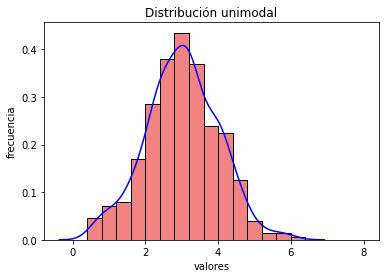
\includegraphics[width=\linewidth]{images/unimodal.png}
    \endminipage\hfill
    \minipage{0.5\textwidth}%
      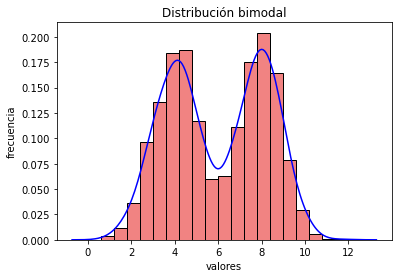
\includegraphics[width=\linewidth]{images/bimodal.png}
    \endminipage
     \caption{Ejemplos de distribuciones de probabilidad.}
\end{figure}

\subsection*{Distribución Bernoulli}

La \textit{distribución Bernoulli} es una distribución de probabilidad aplicada a una variable aleatoria discreta, la cual solo puede tomar dos resultados mutuamente excluyentes (éxito o fracaso).\\

\begin{definition}[Distribución Bernoulli]
Una variable aleatoria unidimensional $X$ sigue una \textit{distribución Bernoulli} de parámetro $p$ si su función de probabilidad viene dada por: $$P(X=x)=\left \{
\begin{array}{l l}
p, & \mbox{si } x = 1, \\
1-p, & \mbox{si } x =0.
\end{array}
\right.$$
\end{definition}\

Escribiremos la distribución como $X \sim Bernoulli(p)$, donde el parámetro $p\in (0,1)$ indica la probabilidad de éxito y $(1-p)$ la probabilidad de fracaso del experimento.\\

\begin{proposition}[Propiedades]
Si $X \sim Bernoulli(p)$, entonces la variable aleatoria $X$ satisface las siguientes propiedades:
\begin{itemize}
    \item $\mathbb{E}[X]=p$.
    \item $\text{Var}(X)=p(1-p)$.
\end{itemize}
\end{proposition}

\clearpage

\subsection*{Distribución de Poisson}

La \textit{distribución de Poisson} es una distribución de probabilidad discreta que modela el número de sucesos raros que ocurren en un determinado periodo de tiempo.\\

\begin{definition}[Distribución de Poisson]
Una variable aleatoria unidimensional $X$ sigue una \textit{distribución de Poisson} de parámetro $\lambda$ si su función de probabilidad viene dada por: $$P(X=x)=\ddfrac{\lambda^xe^{-\lambda}}{x!},$$
donde $x=0,1,\dots$ es el número de ocurrencias del evento o fenómeno.
\end{definition}\

Escribiremos la distribución como $X \sim Poisson(\lambda)$, donde el parámetro $\lambda > 0$ representa el número de veces que se espera que ocurra el fenómeno durante un intervalo dado.\\


\begin{proposition}
Si $X \sim Poisson(\lambda)$, entonces la variable aleatoria $X$ satisface las siguientes propiedades:
\begin{itemize}
    \item[1.] $\mathbb{E}[X]=\lambda$.
    \item[2.] $\text{Var}(X)=\lambda$.
    \item[3.] La moda de $X$ es $\lfloor \lambda \rfloor$ (el mayor entero menor que $\lambda$).
\end{itemize}
\end{proposition}

\begin{proof}
  Demostraremos la propiedad 1 utilizando la definición de $\mathbb{E}[X]$. \\
  \begin{equation*}
  \begin{split}
  \mathbb{E}[X]&=\sum_{x=0}^\infty x \left(\ddfrac{\lambda^x e^{-\lambda}}{x!}\right)\\
  &=\lambda e^{-\lambda} \sum_{x=1}^\infty \ddfrac{\lambda^{x-1}}{(x-1)!}\\
  &\overset{(*)}{=}\lambda e^{-\lambda} \sum_{y=0}^\infty \ddfrac{\lambda^{y}}{y!}\\
  &=\lambda e^{-\lambda} e^{\lambda}\\
  &=\lambda.
  \end{split}
  \end{equation*} donde en $(*)$ hemos cambiado $(x-1)$ por $y$.\\
  
  Para la propiedad 2, sabiendo que
  \begin{equation}\label{eq:varxprop}
    \text{Var}(X)=\mathbb{E}[X^2]-\mathbb{E}[X]^2=\mathbb{E}[X(X-1)]+\mathbb{E}[X]-\mathbb{E}[X]^2.
  \end{equation}
  
  Procederemos con el cálculo de $\mathbb{E}[X(X-1)]$. \begin{equation*}
  \begin{split}
 \mathbb{E}[X(X-1)]&=\sum_{x=0}^\infty x(x-1)\left(\ddfrac{\lambda^x e^{-\lambda}}{x!}\right)\\
 &=\lambda^2 e^{-\lambda} \sum_{x=2}^\infty \ddfrac{\lambda^{x-2}}{(x-2)!}\\ &\overset{(*)}{=}\lambda e^{-\lambda} \sum_{y=0}^\infty \ddfrac{\lambda^{y}}{y!}\\
 &=\lambda^2 e^{-\lambda} e^{\lambda}\\
 &=\lambda^2.
  \end{split}
  \end{equation*} donde en $(*)$ hemos cambiado $(x-2)$ por $y$.\\
  
  Sustituyendo en la Ecuación (\ref{eq:varxprop}) concluimos que, $\text{Var}(X)=\lambda^2+\lambda-\lambda^2=\lambda.$
\end{proof}\

\begin{proposition}
Si $X \sim Poisson(\lambda)$, donde $X$ es una variable aleatoria que representa el número de sucesos raros en una unidad de tiempo e $Y$ es una variable aleatoria que representa el número de dichos sucesos raros en un tiempo $t$, se tiene que $$Y \sim Poisson(t\lambda).$$
\end{proposition}\

\begin{example} \label{ex:ejpoisson}
En un instituto, el número medio de suspensos por clase es de $2.4$. Es decir, si $X$ es el número de suspensos por clase, entonces $$X \sim Poisson(2.4).$$ 

¿Cuál es la probabilidad de que en una clase no haya suspensos? $$P(X=0)=\ddfrac{2.4^0 e^{-2.4}}{0!}=e^{-2.4}=0.09.$$

¿Cuál es la probabilidad de que en 3 clases haya exactamente 6 suspensos?

Sea $Y$ el número de suspensos en 3 clases. Sabemos que: $$Y \sim Poisson(2.4\cdot 3)=Poisson(7.2)$$ $$P(Y=6)=\ddfrac{7.2^6 e^{-7.2}}{6!}=e^{-3.4}=0.14.$$
\end{example}\

\begin{figure}[h]
    \minipage{0.5\textwidth}
      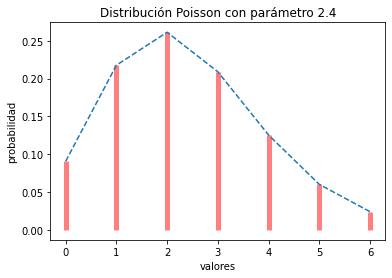
\includegraphics[width=\linewidth]{images/poisson1.png}
    \endminipage\hfill
    \minipage{0.5\textwidth}%
      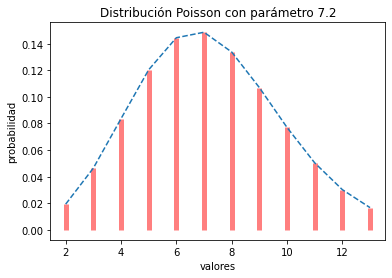
\includegraphics[width=\linewidth]{images/poisson2.png}
    \endminipage
     \caption{Distribuciones calculadas en el Ejemplo \ref{ex:ejpoisson}.}
\end{figure}

\subsection*{Distribución Normal}

La \textit{distribución normal} o  \textit{distribución de Gauss} se utiliza para representar variables aleatorias de valor real cuyas distribuciones son desconocidas.\\

\begin{definition}[Distribución normal]
Una variable aleatoria unidimensional $X$ sigue una \textit{distribución normal} o \textit{gaussiana} de parámetros $\mu, \sigma$, si su función de densidad $f\colon \R \to \R$ viene dada por: $$f(x)=\ddfrac{1}{\sigma \sqrt{2\pi}} \ e^{-\frac{1}{2}(\frac{x-\mu}{\sigma})^2},$$
donde $\mu,\sigma\in \R$.
\end{definition}\

Donde escribiremos la distribución como $X \sim \mathcal{N}(\mu, \sigma^2)$, donde recordemos el parámetro $\mu$ se refiere a la media y $\sigma$ a la desviación estándar de la variable aleatoria.\\

\begin{proposition} \label{prop:propnormal}
Si $X \sim \mathcal{N}(\mu, \sigma^2)$, entonces la variable aleatoria $X$ satisface las siguientes propiedades :
\begin{itemize}
    \item La distribución es simétrica respecto a $\mu$.
    \item $P(\mu-\sigma < X < \mu+\sigma)\approx 0.683.$
    \item $P(\mu-2\sigma < X < \mu+2\sigma)\approx 0.955.$
    \item $P(\mu-3\sigma < X < \mu+3\sigma)\approx 0.997.$
    \item La moda de $X$ coincide con $\mu$.
\end{itemize}
\end{proposition}\

Como consecuencia de la primera propiedad de la Proposición \ref{prop:propnormal}, podemos relacionar todas las variables aleatorias normales con la distribución $\mathcal{N}(0,1)$.\\

\begin{proposition}[Estandarización de variables aleatorias normales]
Sea $X$ una variable aleatoria tal que $X \sim \mathcal{N}(\mu, \sigma^2)$, entonces: $$Z=\ddfrac{X-\mu}{\sigma} \sim \mathcal{N}(0,1),$$
donde $\mathcal{N}(0,1)$ es la distribución normal estándar.
\end{proposition}\

\begin{figure}[h]
	\centering
	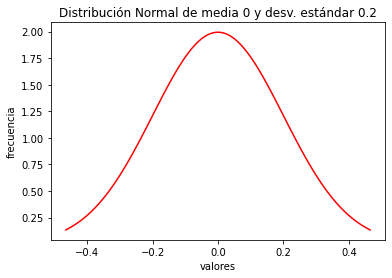
\includegraphics[width=9.8cm]{distnormal.png}
	\caption{Ejemplo de una distribución normal.}
    \label{fig:distrnormal}
\end{figure}\

\begin{definition}[Media muestral]
Sean $X_1,\dots,X_n$ variables aleatorias obtenidas a partir de $X$ y que siguen su misma distribución, se define la \textit{media muestral} como:
$$\overline{X}_n=\frac{1}{n}\sum_{i=1}^n X_i.$$
\end{definition}\

La importancia de la distribución normal reside principalmente en el Teorema central del límite que trata sobre la distribución de la media muestral para variables aleatorias independientes e idénticamente distribuidas (i.i.d) y garantiza una distribución aproximadamente normal cuando $n$ es lo suficientemente grande.\\

\begin{theorem}[Teorema central del límite] \label{th:thcentral}
Sean $X_1,X_2,\dots,X_n$ variables aleatorias i.i.d con media $\mu$ y desviación estándar $\sigma^2$ (ambas finitas). Con $n$ suficientemente grande, se tiene que $$\frac{\overline{X}-\mu}{\sigma / \sqrt{n}}\sim \mathcal{N}(0,1).$$
\end{theorem}

\clearpage

Finalmente, podemos relacionar las dos distribuciones estudiadas aproximando la distribución de Poisson mediante la distribución normal estándar a partir de la siguiente relación:\\

\begin{proposition}
Sea $X$ una variable aleatoria tal que $X \sim Poisson(\lambda)$ con $\lambda$ suficientemente grande, entonces: $$\ddfrac{X-\lambda}{\sqrt{\lambda}}\sim \mathcal{N}(0,1).$$
\end{proposition}\

Como una extensión del caso unidimensional, aparece el caso de distribución normal multivariante que definiremos a continuación.\\

\begin{definition}[Distribución normal multivariante]
Sea un vector aleatorio $\nm{X}=(X_1,\dots,X_n)^T$ diremos que sigue una \textit{distribución normal multivariante} de parámetros $\bm{\mu},\bm{\Sigma}$ si su función de densidad $f\colon \Rn \to \R$ viene dada por: $$f(x)=\ddfrac{1}{\sqrt{\text{det}(2\pi \bm{\Sigma})}}e^{-\frac{1}{2}(x-\bm{\mu})^T\bm{\Sigma}^{-1}(x-\bm{\mu})},$$
donde $\bm{\mu}\in \Rn$ y $\bm{\Sigma}\in \mathcal{M}(\R)$.
\end{definition}\

Escribiremos la distribución como $\nm{X} \sim \mathcal{N}(\bm{\mu}, \bm{\Sigma})$, donde recordemos el parámetro $\bm{\mu}$ se refiere al vector de las medias de la distribución y $\bm{\Sigma}$ a la matriz de covarianzas.

\subsection*{Distribución Uniforme}

\begin{definition}[Distribución uniforme discreta]
Una variable aleatoria discreta $X$ con posibles valores $\{x_1,\dots,x_n\}$ diremos que sigue una \textit{distribución uniforme} si: $$P(X=x_i)=\frac{1}{n}, \ \text{para todo} \ i=1,\dots,n.$$
\end{definition}\

\begin{definition}[Distribución uniforme continua]
Una variable aleatoria continua $X$ sigue una \textit{distribución uniforme} en el intervalo $(a,b)$ si su función de densidad viene dada por: $$f(x)=\left \{
\begin{array}{l l}
\frac{1}{b-a}, & \mbox{si } x \in (a,b), \\
0, & \mbox{si } x \notin (a,b).
\end{array}
\right.$$
\end{definition}\

Escribiremos la distribución como $X \sim U(a,b)$, donde la variable aleatoria queda definida por los extremos del intervalo, es decir, $a$ y $b$ son sus parámetros.\\

\begin{proposition}[Propiedades]
Si $X \sim U(a,b)$, entonces la variable aleatoria $X$ satisface las siguientes propiedades:
\begin{itemize}
    \item $\mathbb{E}[X]=\frac{a+b}{2}$.
    \item $\text{Var}(X)=\frac{(b-a)^2}{12}$.
    \item La moda de $X$ es cualquier valor en $(a,b)$.
\end{itemize}
\end{proposition}


\subsection*{Distribución Gamma}

\begin{definition}[Distribución gamma]
Una variable aleatoria continua $X$ sigue una \textit{distribución gamma} de parámetros $\alpha$ y $\lambda$ si su función de densidad viene dada por: $$f(x)=\ddfrac{\lambda^{\alpha}x^{\alpha-1}e^{-\lambda x}}{\Gamma(\alpha)}.$$
donde $\Gamma$ es la \textit{función gamma} definida como $\Gamma(\alpha)=\displaystyle \int_0^{+\infty}x^{\alpha-1}e^{-x} \ dx$.
\end{definition}\

Escribiremos la distribución como $X \sim \Gamma(\alpha,\lambda)$, donde la variable aleatoria queda definida por los parámetros $\alpha,\lambda > 0$.\\

\begin{proposition}[Propiedades]
Si $X \sim \Gamma(\alpha,\lambda)$, entonces la variable aleatoria $X$ satisface las siguientes propiedades:
\begin{itemize}
    \item $\mathbb{E}[X]=\frac{\alpha}{\lambda}$.
    \item $\text{Var}(X)=\frac{\alpha}{\lambda^2}$.
\end{itemize}
\end{proposition}\

\begin{definition}[Distribución gamma inversa]
Una variable aleatoria continua $X$ sigue una \textit{distribución gamma inversa} de parámetros $\alpha$ y $\lambda$ si su función de densidad viene dada por: $$f(x)=\ddfrac{\lambda^\alpha x^{-(\alpha+1)} e^{\frac{-\lambda}{x}}}{\Gamma(\alpha)}.$$
\end{definition}

\chapter{Estadística paramétrica} \label{ch:estapar}

La \textit{estadística paramétrica} es una rama de la inferencia estadística que comprende los procedimientos estadísticos y de decisión basados en distribuciones conocidas, que vienen determinadas por un número finito de parámetros. En este capítulo definiremos algunos conceptos de este campo, que utilizaremos a lo largo del trabajo, y que son tratados en mayor profundidad en \cite{inferencia2012}.\\

\begin{definition}[Muestra aleatoria simple]
Sea una variable aleatoria $X$ que sigue una distribución de probabilidad determinada. Definimos una \textit{muestra aleatoria simple} de tamaño $n$ como un conjunto de variables aleatorias $(X_1,\dots,X_n)$, independientes e idénticamente distribuidas, obtenidas a partir de la distribución de $X$.
\end{definition}\

\begin{definition}[Estadístico muestral]
Un \textit{estadístico de una muestra} aleatoria simple $(X_1,\dots,X_n)$, es una función medible $T\colon \R^n \to \R$, que se aplica a la muestra, lo denotaremos como $T(X_1,\dots,X_n)$.\\
\begin{remark}
Un \textit{estadístico muestral} también es una variable aleatoria.
\end{remark}
\end{definition}\

\begin{example}
Algunos estadísticos muestrales más comunes son:
\begin{itemize}
    \item \textbf{Media muestral} ($\overline{X}$), $$ T(X_1,\dots,X_n)=\frac{1}{n}\sum_{i=1}^n X_i.$$
    \item \textbf{Varianza muestral} ($\mathcal{S}^2$),  $$ T(X_1,\dots,X_n)=\frac{1}{n}\sum_{i=1}^n (X_i-\overline{X})^2.$$
    \item \textbf{Menor valor muestral}, $$ T(X_1,\dots,X_n)=\min (X_1,\dots,X_n).$$
    \item \textbf{Mayor valor muestral},  $$ T(X_1,\dots,X_n)=\max (X_1,\dots,X_n).$$
\end{itemize}
\end{example}\

Particularizando el uso del término estadístico muestral, aparece el concepto de estimador.\\

\begin{definition}[Estimador]
Un \textit{estimador} es un estadístico cuyos valores se utilizan para obtener información de un parámetro desconocido $\btheta$, lo denotaremos como $\htheta \mst$.
\end{definition}

\section{Propiedades del estimador}

A continuación definiremos algunas propiedades que nos permitirán comparar diferentes estimadores de un mismo parámetro, y nos informarán de la calidad de su estimación.\\

\begin{definition}[Estimador insesgado]
Si $\htheta$ es un estimador del parámetro $\btheta$, la diferencia $$\text{sesgo}(\htheta)=\mathbb{E}[\htheta]-\btheta,$$
se denomina \textit{sesgo} del estimador $\htheta$ como estimador de $\btheta$. Cuando el sesgo es nulo para cualquier valor del parámetro, es decir, si $$\mathbb{E}[\htheta]=\btheta, \ \text{para todo} \ \btheta \in \Theta,$$
diremos que el estimador $\htheta$ es \textit{insesgado} para $\btheta$.
\end{definition}\

\begin{example} \label{ex:sesgonul}
Sea $X_1,\dots,X_n$ una muestra aleatoria de una variable aleatoria $X$. Si el parámetro de interés es la media $\mu=\mathbb{E}[X]$, podemos utilizar la media muestral para estimarlo. Calculamos su sesgo: $$\text{sesgo}(\overline{X})=\mathbb{E}[\overline{X}]-\mu=\frac{1}{n}\sum_{i=1}^n \mathbb{E}[X_i]-\mu=\mu-\mu=0,$$
demostrando que $\overline{X}$ es un estimador insesgado para $\mu$.
\end{example}\

\begin{definition}[Estadístico suficiente]
Sea $T=T\mst$ un estadístico muestral se dice \textit{suficiente} para el parámetro $\btheta$ si la distribución condicional de la muestra $\mst$ dado el valor de $T\mst$ no depende del parámetro a estimar $\btheta$.
\end{definition}\


\begin{definition}[Estimador suficiente]
Un estimador $\htheta$ es \textit{suficiente} si es un estadístico suficiente.
\end{definition}\

A partir de la propiedad de suficiencia aparece el Teorema de factorización de Fisher-Neyman, que nos ofrece una caracterización de estadístico suficiente.\\


\begin{theorem}[Teorema de factorización de Fisher-Neyman]
Sea $T=T\mst$ un estadístico muestral si la función de densidad es $f_{\btheta}(x)$, entonces $T$ es suficiente para $\btheta$ si, y solo si, podemos encontrar $g,h\colon \R^n \to \R$ funciones no negativas tal que $$f_{\btheta}(x)=h(x)g_{\btheta}(T(x)).$$
es decir, podemos factorizar la función de densidad como un producto de dos funciones: $h$ que no depende de $\btheta$ y $g$ que depende de $\btheta$ y de $x$ solo a través de $T(x)$.
\end{theorem}\

El tamaño de la muestra es un factor determinante en la estimación, a raíz de esto, surge el término de estimador \textit{consistente}. En la definición de consistencia se usan nociones de \textit{convergencia en probabilidad}, que comentaremos a continuación.\\

\begin{definition}[Convergencia en probabilidad]
Una sucesión de variables aleatorias $\{X_n\}$ \textit{converge en probabilidad} a la variable aleatoria $X$ si para todo $\epsilon>0$ entonces, $$\lim_{n\to +\infty}P([X_n-X]>\epsilon)=0.$$
Lo denotaremos como $X_n \overset{P}{\to} X.$
\end{definition}\

\begin{definition}[Estimador consistente]
Sea $\htheta_n$ un estimador del parámetro $\btheta$ para una muestra de tamaño $n$. Diremos que el estimador $\htheta_n$ es \textit{consistente} si, cuando $n\to +\infty$, se verifica que $$\htheta_n \overset{P}{\to} \btheta.$$
\end{definition}\

\begin{definition}[Estimador asintóticamente insesgado]
Sea $\htheta_n$ un estimador del parámetro $\btheta$ para una muestra de tamaño $n$. Diremos que el estimador $\htheta_n$ es \textit{asintóticamente insesgado} si, cuando $n\to +\infty$, se verifica que $$\text{sesgo}(\htheta_n) \to 0.$$
\end{definition}\

\begin{corollary} \label{cor:lemaestima}
Sea $\htheta_n$ un estimador del parámetro $\btheta$ para una muestra de tamaño $n$. Si $\htheta_n$ es asintóticamente insesgado y además si $n\to +\infty$ se cumple que $$\text{Var}(\htheta_n)\to 0.$$
entonces, el estimador $\htheta_n$ es consistente.
\end{corollary}\

Finalmente enunciaremos la propiedad de \textit{eficiencia} de un estimador.\\

\begin{definition}[Estimador eficiente] \label{def:efvar}
Sean $\htheta_1$ y $\htheta_2$ dos estimadores del parámetro $\btheta$. Se dice que $\htheta_1$ es más \textit{eficiente} que $\htheta_2$ si verifica que $$\text{Var}(\htheta_1)<\text{Var}(\htheta_2).$$
\end{definition}\

\begin{example} \label{ex:eficienciaex}
Sea $X \sim U(0,b)$.
Como $X$ sigue una distribución uniforme, entonces: $$\mathbb{E}[X]=\frac{b}{2} \quad \text{ y } \quad \text{Var}(X)=\frac{b^2}{12}.$$
Sean dos estimadores insesgados:
$$\bm{\hat{b}_1}(X_1,\dots,X_{5})=\overline{X}.$$
$$\bm{\hat{b}_2}(X_1,\dots,X_{5})=\max \{X_1,\dots,X_5\}.$$\\
A continuación veremos cual de los dos estimadores es más eficiente, procederemos calculando la varianza de cada uno de ellos:\\

\begin{itemize}
    \item Cálculo de la varianza de $\bm{\hat{b}_1}$: $$\text{Var}(\bm{\hat{b}_1})=\text{Var}(\overline{X})=\frac{\text{Var}(X)}{n}=\frac{b^2/12}{5}=\frac{b^2}{60}.$$
    \item Cálculo de la varianza de $\bm{\hat{b}_2}$: $$\mathbb{E}\left[\bm{\hat{b}_2}^2\right]=\int_{0}^b x^2 f_{\bm{\hat{b}_2}^2}(x) \ dx=\int_{0}^b x^2 \ \frac{5x^4}{b^5} \ dx=\frac{5}{b^5}\int_{0}^b x^6 \ dx=\frac{5}{b^5}\left[\frac{x^7}{7}\right]_{0}^b=\frac{5}{7}b^2.$$
    Como $\bm{\hat{b}_2}$ es un estimador insesgado, entonces $\mathbb{E}[\bm{\hat{b}_2}]=b$.
    $$\text{Var}\left(\bm{\hat{b}_2}\right)=\mathbb{E}\left[\bm{\hat{b}_2}^2\right]-\mathbb{E}\left[\bm{\hat{b}_2}\right]^2=\frac{5}{7}b^2-b^2=-\frac{2}{7}b^2.$$
\end{itemize}\

Concluimos que $\bm{\hat{b}_2}$ es más eficiente que $\bm{\hat{b}_1}$ ya que: $$\text{Var}(\bm{\hat{b}_2})= -\frac{2b^2}{7} < \frac{b^2}{60}=\text{Var}(\bm{\hat{b}_1}).$$
\end{example}

\clearpage

\section{Criterios de evaluación} \label{sec:coeficientedet}

\begin{definition}[Error cuadrático medio]
El \textit{error cuadrático medio} (ECM) de un estimador $\htheta$ con respecto al parámetro desconocido $\btheta$  se define como: $$\text{ECM}(\htheta)=\mathbb{E}[(\htheta-\btheta)^2].$$
\end{definition}\

\begin{proposition}
Sea $\htheta$ un estimador de $\btheta$. Se cumple que:
$$\text{ECM}(\htheta)=\text{Var}(\htheta)+\text{sesgo}(\htheta)^2.$$
\end{proposition}

\begin{proof}
 $$\text{ECM}(\htheta)=\mathbb{E}[(\htheta-\btheta)^2]=\mathbb{E}[\htheta^2+\btheta^2-2\htheta \btheta]=\mathbb{E}[\htheta^2]+\btheta^2-2\btheta\mathbb{E}[\htheta].$$\\
Sumando y restando $\mathbb{E}[\htheta]^2$ en la expresión anterior, obtenemos:\\
  \begin{equation*}
  \begin{split}
 \text{ECM}(\htheta)&=\mathbb{E}[\htheta^2]+\btheta^2-2\btheta\mathbb{E}[\htheta]\textcolor{blue}{+\mathbb{E}[\htheta]^2-\mathbb{E}[\htheta]^2}\\
 &=(\mathbb{E}[\htheta^2]-\mathbb{E}[\htheta]^2)+(\btheta^2+\mathbb{E}[\htheta]^2-2\btheta\mathbb{E}[\htheta])\\
 &=(\mathbb{E}[\htheta^2]-\mathbb{E}[\htheta]^2)+(\btheta+\mathbb{E}[\htheta])^2\\
 &=\text{Var}(\htheta)+\text{sesgo}(\htheta)^2.
  \end{split}
  \end{equation*} 
\end{proof}

El ECM involucra las propiedades de insesgadez y
eficiencia; ya que cuanto más cerca esté la esperanza de un estimador del parámetro, y cuanto más pequeña sea su varianza, menor será su error cuadrático medio.\\

\begin{proposition} \label{prop:varecm}
Si $\htheta$ es un estimador insesgado, entonces: $$\text{ECM}(\htheta)=\text{Var}(\htheta).$$ 
\end{proposition}\

A partir del concepto de ECM se define el concepto de \textit{raíz del error cuadrático medio}, que es una medida de uso frecuente de las diferencias entre los valores predichos por un estimador y los valores observados, y que utilizaremos en la práctica para evaluar modelos de predicción.\\

\begin{definition}[Raíz del error cuadrático medio]
La \textit{raíz del error cuadrático medio} (RMSE) de un estimador $\htheta$ con respecto al parámetro desconocido $\btheta$ se define como: $$\text{RMSE}(\htheta)=\sqrt{\text{ECM}(\htheta)}=\sqrt{\mathbb{E}[(\htheta-\btheta)^2]}.$$
\end{definition}\

\begin{remark}
Si $\htheta$ es insesgado, por la Proposición \ref{prop:varecm}: $$\text{RMSE}(\htheta)=\sqrt{\text{Var}(\htheta)}=\sigma.$$
\end{remark}

Estas medidas de evaluación pueden particularizarse para modelos de predicción a partir del siguiente resultado:\\

\begin{proposition}
Sea $\hat{\nm{y}}$ un vector de $n$ predicciones e $\nm{y}$ el vector con las etiquetas reales de las mismas, entonces podemos calcular las medidas de de evaluación anteriores como: $$\text{ECM}=\frac{1}{n}\sum_{i=1}^n (\hat{\nm{y}}_i-\nm{y}_i)^2.$$ $$\text{RMSE}=\sqrt{\text{ECM}}=\sqrt{\frac{1}{n}\sum_{i=1}^n (\hat{\nm{y}}_i-\nm{y}_i)^2}.$$
\end{proposition}\

Finalmente definiremos otro posible criterio de evaluación para una distribución dada por un estimador.\\

\begin{definition}[Coeficiente de determinación]
El \textit{coeficiente de determinación} ($R^2$) es un estadístico que determina la calidad de un modelo para predecir resultados y medir la variación que puede ser explicada por el mismo. En regresión lineal, sean $X,Y$ dos variables aleatorias, el coeficiente $R^2$ se calcula como: $$R^2=\frac{\sigma^2_{XY}}{\sigma^2_X \sigma^2_Y}.$$
\end{definition}\

\begin{proposition}
Sea $\hat{\nm{y}}$ un vector de $n$ predicciones e $\bar{\nm{y}}$ la media del vector con las etiquetas reales, podemos calcular su coeficiente de determinación a partir de la siguiente expresión: $$R^2=\ddfrac{\sum_{i=1}^n (\hat{\nm{y}}_i-\bar{\nm{y}})^2}{\sum_{i=1}^n (\nm{y}_i-\bar{\nm{y}})^2}.$$
\end{proposition}


\chapter{Teoría de grafos} \label{ch:teorgraf}

En este capítulo incluiremos algunos conceptos fundamentales, que nos serán útiles en la construcción de los modelos causales, y que funcionan como base del concepto de equidad contrafactual que trataremos a lo largo del trabajo. La referencia básica de este capítulo es el libro de \cite{graphtheory2001}.

\section{Grafos, nodos y aristas}

\begin{definition}[Par ordenado]
Un \textit{par ordenado} es una pareja de elementos, en la que los elementos vienen distinguidos por su orden. El par ordenado donde el primer elemento es $a$ y el segundo $b$ se denota como $(a,b)$. Si el orden no es relevante, lo llamaremos \textit{par no ordenado} y lo denotaremos $\{a,b\}$. En este caso, es claro que $\{a,b\}=\{b,a\}$.
\end{definition}\

\begin{definition}[Grafo]
Un \textit{grafo} $G = (V,E)$ es un conjunto no vacío de vértices o nodos $V$ y aristas $E \subset V\times V$ entre ellos.
Si $E$ consta de pares ordenados de vértices lo llamaremos \textit{grafo dirigido}, si en otro caso $E$ consta de pares no ordenados, lo llamaremos \textit{grafo no dirigido}.
\end{definition}\

\begin{figure}[h]
\centering
\begin{tikzpicture}[
  node distance=1cm and 1cm,
  mynode/.style={draw,circle,text width=0.5cm,align=center}
]

\node[mynode] (a) {A};
\node[mynode,below =of a] (b) {B};
\node[mynode, right=of a] (d) {D};
\node[mynode,below =of d] (c) {C};

\node[mynode, right=of d] (e) {A};
\node[mynode,below =of e] (f) {B};
\node[mynode, right=of e] (g) {D};
\node[mynode,below =of g] (h) {C};

\path (a) edge[-latex] (d)
(a) edge[-latex] (b)
(c) edge[latex-] (b)
(c) edge[latex-] (d);

\draw (e) -- (f) -- (h) -- (g) -- (e);

\end{tikzpicture}
\caption{Ejemplo de un grafo dirigido y un grafo no dirigido, respectivamente.}
\label{fig:dirungraphs}
\end{figure}\

\begin{definition}[Camino]
En un grafo dirigido $G=(V,E)$, un \textit{camino} $A \to B$ es una secuencia de vértices $\{A = v_0,v_1,\dots,v_{n-1}, v_n = B\}$ donde $(v_i, v_{i+1}) \in E \ \text{para todo} \ i \in
\{0,\dots ,n-1\}$. Si $G$ es un grafo no dirigido, $A\to B$ es un \textit{camino} si $\{v_i,v_{i+1}\} \in E \ \text{para todo} \ i \in \{0,\dots,n-1\}$.
\end{definition}\

\begin{definition}[Grafo acíclico dirigido]
Un \textit{grafo acíclico dirigido} es un grafo dirigido que no tiene ciclos, es decir, que para cada nodo $v\in V$, no existe ningún camino que empiece y termine en $v$. Si un grafo no es acíclico lo llamaremos \textit{ciclo}.
\end{definition}\

\begin{figure}[h]
\centering
\begin{tikzpicture}[
  node distance=1cm and 1cm,
  mynode/.style={draw,circle,text width=0.5cm,align=center}
]

\node[mynode] (a) {A};
\node[mynode,below =of a] (b) {B};
\node[mynode, right=of a] (d) {D};
\node[mynode,below =of d] (c) {C};

\node[mynode, right=of d] (e) {A};
\node[mynode,below =of e] (f) {B};
\node[mynode, right=of e] (g) {D};
\node[mynode,below =of g] (h) {C};

\path (a) edge[-latex] (d)
(a) edge[-latex] (b)
(c) edge[latex-] (b)
(c) edge[latex-] (d);

\path (e) edge[-latex] (f)
(g) edge[-latex] (e)
(h) edge[latex-] (f)
(g) edge[latex-] (h);


\end{tikzpicture}
\caption{Ejemplo de un grafo acíclico dirigido y un ciclo dirigido, respectivamente.}
\label{fig:acigraphs}
\end{figure}

\begin{example}
Podemos ver que el grafo de la izquierda de la Figura \ref{fig:acigraphs} es acíclico puesto que sea $v\in \{A,B,C,D\}$ no existe ningún camino que revisite $v$. Por otro lado, el grafo de la derecha es un ciclo, ya que el camino $A\to B \to C \to D \to A$ es directo y empieza y termina en $A$.
\end{example}\

\begin{definition}[Bucle]
Sea $G=(V,E)$ un grafo y $v\in V$ un vértice del mismo. Diremos que $v$ tiene un \textit{bucle} si $(v,v)\in E$.
\end{definition}\

\begin{definition}[Grafo simple]
Diremos que $G$ \textit{grafo simple} si no posee bucles ni ninguna de sus aristas relacionan al mismo par de vértices. Llamaremos a $G$ \textit{multigrafo} si, y solo si, no es un grafo simple.
\end{definition}

\section{Estructura de un grafo}

Ahora definiremos algunas relaciones entre nodos en un grafo acíclico dirigido.\\

\begin{definition}[Ancestros y descendientes de un nodo] \label{def:ancestro}
Sean $A,B$ dos vértices de un grafo dirigido $G$. Si $A \to B$ es un camino dirigido y $B \not \to A$ (no existe un camino dirigido de $B$ a $A$), entonces diremos que $A$ es el \textit{ancestro} de $B$ y $B$ es \textit{descendiente} de $A$.
\end{definition}\

\begin{example}
En el grafo de la derecha de la Figura \ref{fig:acigraphs}, el nodo $A$ es un ancestro de  $B$, $D$ y $C$. Por otro lado, el nodo $C$ es un descendiente de $A$, $B$ y $D$.
\end{example}

\clearpage

\begin{definition}[Padres e hijos de un nodo]
Particularizando la Definición \ref{def:ancestro}, definimos a los \textit{padres} de un nodo $A$ como el conjunto de nodos $pa(A)$ tal que existe una arista dirigida para cada nodo de $pa(A)$ hacia $A$, la noción inversa de padres define el concepto de \textit{hijos} a los que denotaremos como $hi(A)$.
\end{definition}\

\begin{definition}[Vecinos de un nodo]
Sea un grafo $G$, definimos los \textit{vecinos} de un nodo como todos los nodos directamente conectados a él. Denotaremos al conjunto de vecinos de un nodo $A$ como $ve(A)$.
\end{definition}\

\begin{figure}[h]
\centering
\begin{tikzpicture}[
  node distance=1cm and 1cm,
  mynode/.style={draw,circle,text width=0.5cm,align=center}
]

\node[mynode] (a) {A};
\node[mynode,below right=of a] (b) {B};
\node[mynode,above right=of b] (c) {C};
\node[mynode,below right=of b] (d) {D};
\node[mynode,below left=of b] (e) {E};
\node[mynode,right=of c] (f) {F};

\path (c) edge[-latex] (a)
(a) edge[-latex] (b)
(b) edge[latex-] (c)
(b) edge[-latex] (e)
(c) edge[-latex] (f)
(b) edge[-latex] (d)
(f) edge[-latex] (d)
;

\end{tikzpicture}
\caption{Ejemplo de grafo acíclico dirigido.}
\label{fig:relations}
\end{figure}

\begin{example}
Para comprender las definiciones anteriores, definiremos los conjuntos de padres, hijos y vecinos del nodo $B$ para la Figura \ref{fig:relations}. $$pa(B)=\{A,C\}, \ \ hi(B)=\{E,D\}, \ \ ve(B)=\{A,C,E,D\}.$$
\end{example}

\ctparttext{\color{black}\begin{center}
Conceptos básicos del aprendizaje automático, formalización de las medidas de equidad y definición de los principales algoritmos de mitigación del sesgo.
\end{center}}
\part{Justicia en Aprendizaje Automático} \label{part:jusaa}


\chapter{Conceptos básicos del Aprendizaje Automático} \label{ch:conceptosaa}

En este capítulo presentaremos algunos conceptos básicos del aprendizaje automático. Definiremos el concepto de aprendizaje supervisado, discutiremos el proceso de creación de modelos predictivos a partir de un conjunto de datos dado y comentaremos las medidas básicas de evaluación de un modelo de clasificación.

\section{¿Qué es el aprendizaje automático?}

\label{sec:queaprendizaje}

El \textit{aprendizaje automático} o \textit{machine learning} se encarga de extraer patrones significativos de un conjunto de datos con el objetivo de inferir en la distribución estadística subyacente (\cite{pattern2006}). Para ello, durante la fase de entrenamiento, aprendemos un modelo a partir de un conjunto de datos de interés seleccionado previamente. Una vez entrenado el modelo, podremos predecir o tomar decisiones sin que el modelo haya sido específicamente programado para esa tarea. Los patrones generales obtenidos a partir del entrenamiento del modelo podrán aplicarse posteriormente a datos no vistos y seguir obteniendo resultados de utilidad. 

A grandes rasgos, consideramos tres tipos de algoritmos de aprendizaje automático: los de aprendizaje supervisado que actúan sobre datos etiquetados, los de aprendizaje no supervisado que actúan sobre datos no etiquetados y los de aprendizaje por refuerzo que actúan en un entorno de ensayo-error. Para nuestro trabajo, nos centraremos en el entorno de \textit{aprendizaje supervisado}. 

\subsection{Aprendizaje supervisado} \label{subsec:ejemplobanco}

Definiremos los componentes del aprendizaje a partir de un ejemplo real: la aprobación de un crédito bancario. En principio, el banco no conoce ninguna fórmula ideal que pueda comunicarle cuando debe aprobar un crédito. El banco utilizará los registros de los clientes anteriores para aprender sobre ellos y encontrar una buena fórmula para la aprobación de las nuevas peticiones de créditos. Cada registro de clientes tiene información relativa al mismo, como pueden ser salario anual, años de residencia, préstamos pendientes, etc. También registra si la aprobación del crédito para ese cliente fue una buena idea, es decir, si le proporcionó o no beneficios a la entidad financiera. Estos datos serán los que guíen la construcción de una fórmula de éxito para la aprobación del crédito que podrá utilizarse con futuros solicitantes.

A continuación, formalizaremos los principales componentes de este problema de aprendizaje. Tenemos el vector de entrada $\nm{x}$ que contiene la información del cliente que se utilizará para tomar la decisión del crédito, la \textit{función objetivo desconocida} $f\colon \mathcal{X}\to \mathcal{Y}$ (fórmula ideal para la aprobación del crédito), donde $\mathcal{X}$ es el conjunto de todas las posibles características e $\mathcal{Y}$ el conjunto de todos los posibles resultados (en este caso, una decisión binaria si/no). Tenemos un \textit{conjunto de datos} consistente en pares de entrada-salida $\mathcal{D}=\{(\nm{x}_1,y_1),\dots,(\nm{x}_n,y_n)\}$ donde cada  $y_i$ viene dado por una función desconocida $y_i=f(\nm{x}_i)$ con $i=1,\dots,n$ (los valores de entrada corresponden a los antiguos clientes y el resultado será la decisión de crédito correcta para ellos en retrospectiva).

Finalmente, contamos con el \textit{algoritmo de aprendizaje} $\mathcal{A}$ que utiliza el conjunto de datos $\mathcal{D}$ para elegir una fórmula $g\colon \mathcal{X}\to \mathcal{Y}$ que mejor aproxime a la función ideal $f$. El algoritmo elegirá $g$ de entre un conjunto de fórmulas candidatas consideradas, al que denominamos \textit{conjunto de hipótesis} $\mathcal{H}$. Por ejemplo, $\mathcal{H}$ podría ser el conjunto de todas las fórmulas lineales de las que el algoritmo elegiría la que mejor ajuste linealmente a los datos.\\

\begin{figure}[h]
	\centering
	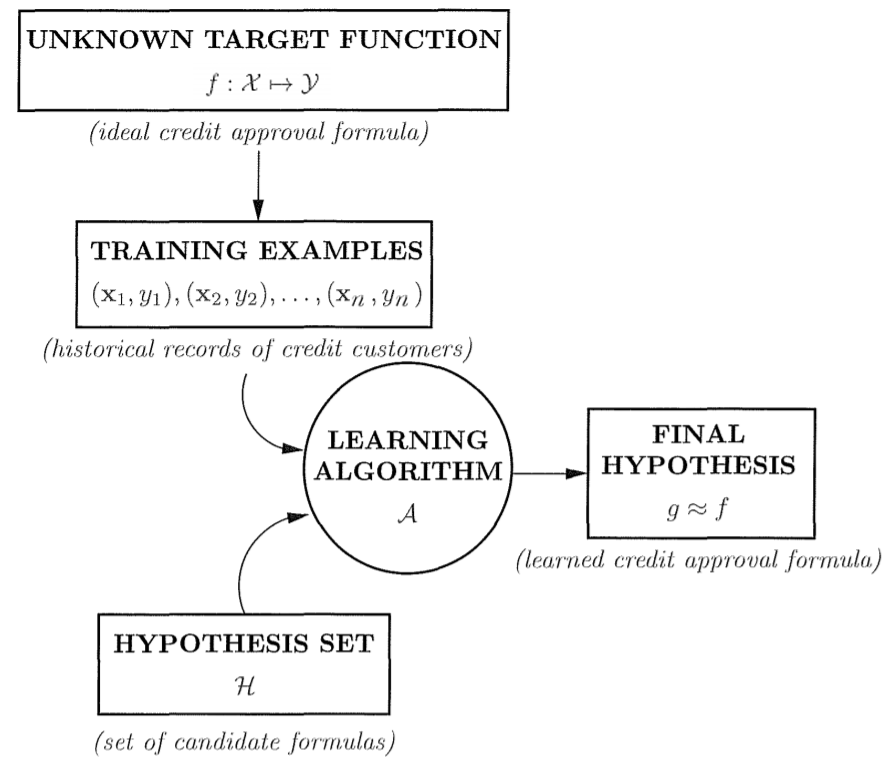
\includegraphics[width=12.6cm]{setup_learning.png}
	\caption{Configuración básica del problema de aprendizaje. (\cite{learning2012})}
    \label{fig:learningesq}
\end{figure}

\clearpage

Cuando un nuevo cliente solicite un crédito, el banco basará su decisión en $g$ (la hipótesis que produjo el algoritmo de aprendizaje) y no en $f$ (la función objetivo ideal) que aún sigue siendo desconocida. La decisión será buena solo en la medida en que $g$ replique $f$. Para ello, el algoritmo elegirá la función $g$ que mejor se ajuste a $f$ en los ejemplos de entrenamiento de clientes anteriores, con la esperanza de que siga coincidiendo con $f$ en los nuevos clientes.

\section{Propiedades del modelo de aprendizaje}

Definiremos algunos conceptos importantes que surgen junto a algunas cuestiones planteadas una vez creado el modelo de aprendizaje (\cite{fairnesslearning2019}). Suponemos un conjunto de datos etiquetado $\mathcal{D}=\{(\nm{x}_1,y_1),\dots,(\nm{x}_n,y_n)\}$. Normalmente los datos $(\nm{x}_1, y_1),\dots, (\nm{x}_n, y_n)$ se extraen de forma independiente e idénticamente distribuida de una población $(\mathcal{X},\mathcal{Y})$.\\

\begin{definition}[Clasificador arbitrario]
Un \textit{clasificador arbitrario} se define como una aplicación $g\colon \mathcal{X} \to \mathcal{Y}$ del conjunto de características $\mathcal{X}$ al conjunto de resultados $\mathcal{Y}$, de forma que $ g(\nm{x})$ es el resultado predicho para el individuo $\nm{x}$.
\end{definition}\

\begin{definition}[Función de pérdida]
Una \textit{función de pérdida} es una función definida como $\ell \colon \mathcal{Y} \times \mathcal{Y} \to \R$ que asigna un valor real no-negativo $\ell(y',y)$ que denota el coste del valor de la predicción $y'$ cuando la etiqueta real es $y$.
\end{definition}\

\begin{definition}[Riesgo empírico]
El \textit{riesgo empírico} de un clasificador arbitrario $g$ con respecto a un conjunto de datos $\mathcal{D}$ dada una función de pérdida $\ell$ se define como: $$R_{\mathcal{D}}(g)=\frac{1}{n}\sum_{i=1}^n \ell(g(\nm{x}_i),y_i).$$
\end{definition}\

\begin{definition}[Minimización del riesgo empírico] \label{def:minrisk}
La \textit{minimización del riesgo empírico} es el problema de optimización que busca encontrar un clasificador $g$ en una familia de funciones $\mathcal{H}$ tal que minimice el riesgo empírico, $$\underset{g\in \mathcal{H}}{\text{arg min}} \  R_{\mathcal{D}}(g).$$
\end{definition}\

La introducción del concepto de minimización del riesgo empírico genera diversas dudas que intentaremos abordar a lo largo de este capítulo y que pueden resumirse en las siguientes tres preguntas:

\begin{itemize}
    \item[1.] ¿Cuál es la clase de funciones $\mathcal{H}$ que deberíamos escoger?
    \item[2.] ¿Cómo resolver de manera eficiente el problema de optimización resultante?
    \item[3.] ¿El clasificador encontrado tendrá el mismo rendimiento sobre los ejemplos del conjunto de entrenamiento que sobre un conjunto de datos de prueba?
\end{itemize}

Estas cuestiones están relacionadas entre sí y dan lugar a los conceptos de \textit{representación, optimización} y \textit{generalización} respectivamente.

\subsection*{Representación}

Normalmente las aplicaciones que utilizan datos con un número relativamente pequeño de características suelen usar \textit{modelos de predicción lineales}. Por otro lado, si los datos de entrenamiento del modelo incluyen imágenes o audio, se suelen aplicar \textit{modelos no lineales}. Las redes neuronales por ejemplo, aplican una secuencia de transformaciones de cada tipo para obtener mejores resultados sobre el conjunto de datos de entrada.

Lo más relevante de la representación para este trabajo es conocer que la mecánica de entrenamiento de un modelo sigue siendo la misma y el modelo utilizado rara vez importa en cuestiones relativas a la equidad.


\subsection*{Optimización}

Si nuestro objetivo es minimizar la exactitud de un clasificador, sería evidente pensar en resolver directamente el problema de minimización del riesgo empírico con respecto a la siguiente función de pérdida: $$\ell(y',y)=\left \{
\begin{array}{l l}
1, & \mbox{si } y\neq y', \\
0, & \mbox{si } y=y'.
\end{array}
\right.$$

El problema de usar esta función es que es difícil de optimizar. Los gradientes de la función de pérdida 0-1 toman el valor cero en todo su dominio, por lo que no podemos esperar que los métodos basados en el gradiente optimicen directamente este tipo de pérdida.

A continuación, veremos una serie de métodos de optimización diferentes que, en determinadas circunstancias, encuentran un mínimo global o local del objetivo de riesgo empírico y aproximan en cierta medida la pérdida 0-1.

\begin{itemize}
    \item \textbf{Pérdida al cuadrado} (\textit{squared loss}) dada por $\frac{1}{2}(y-y')^2$. La minimización empírica del riesgo con esta función de pérdida equivale a la regresión lineal por mínimos cuadrados. 
    \item \textbf{Pérdida de bisagra} (\textit{hinge loss}) se expresa como el $\max\{1-yy',0\}$. Los algoritmos SVM se refieren a la minimización empírica del riesgo con esta función junto con la regularización $\ell_2$.
    \clearpage
    \item \textbf{Pérdida logística} (\textit{logistic loss}) definida como: $$\left \{
    \begin{array}{l l}
    -\log(\sigma(y')), & \mbox{si } y=1, \\
    -\log(1-\sigma(y')), & \mbox{si } y=-1.
    \end{array}
    \right.$$
    Donde $\sigma(y')=1/(1+e^{-y'})$ es la función logística. La minimización empírica del riesgo con esta función de pérdida equivale a la regresión logística. 
\end{itemize}

La elección de la función de pérdida se realizará comparando los rendimientos de las diferentes aproximaciones mediante prueba y error, eligiendo la que mejor funcione en cada caso.

\subsection*{Generalización}

La generalización en el aprendizaje automático hace referencia a cómo de bueno es un modelo predictivo que etiqueta correctamente datos con los que ha entrenado previamente realizando la misma tarea sobre un nuevo conjunto de datos que sigue la misma distribución de la que se extrajeron los datos de entrenamiento.

No obstante, incluso los modelos más avanzados suelen funcionar peor cuando los datos de prueba se extraen de una distribución que difiere ligeramente de la seguida por los datos de entrenamiento. Un ejemplo de ello fue el caso de la creación de un nuevo conjunto de pruebas para la base de datos ImageNet (\cite{generalize2019}).

\section{Creación de modelos de aprendizaje}

Dado el esquema de configuración del problema de aprendizaje supervisado de la Figura \ref{fig:learningesq} discutiremos la creación de un modelo simple de aprendizaje (\cite{learning2012}). Sea $\mathcal{X}=\R^d$ el espacio de entrada, donde $\R^d$ es el espacio euclídeo $d$-dimensional y sea $\mathcal{Y}=\{-1,1\}$ el espacio de salida denotando una decisión binaria (si/no). En el ejemplo de concesión de crédito, las diferentes coordenadas del vector $\nm{x}\in \mathcal{X}$ corresponden a los datos relativos del individuo que solicita el crédito. La salida binaria $y$ corresponde a la aprobación o denegación del préstamo. Especificamos el conjunto de hipótesis $\mathcal{H}$ mediante una forma funcional común a todas las hipótesis $h\in \mathcal{H}$. La forma funcional $h(\nm{x})$ elegida, asigna pesos diferentes a cada coordenada del vector $\nm{x}$, reflejando su importancia en la decisión del problema. Las coordenadas ponderadas se combinan para formar una puntuación y el resultado se compara con un valor umbral previamente establecido. Si el solicitante supera el umbral, el crédito es aprobado, si no, es denegado: $$\text{Aprobar crédito si } \sum_{i=1}^d w_ix_i > \text{ umbral},$$ $$\text{Denegar crédito si } \sum_{i=1}^d w_ix_i < \text{ umbral}.$$

Esta fórmula se puede escribir de forma más compacta como 
\begin{equation} \label{eq:sign-6}
h(\nm{x})=\text{sign}\left(\left( \sum_{i=1}^d w_ix_i\right)+b \right),
\end{equation}


donde $x_1,\dots,x_d$ son los componentes del vector $\nm{x}$; $h(\nm{x})=1$ significa la aprobación del crédito y $h(\nm{x})=-1$ significa la denegación del crédito; $\text{sign}(s)=1$ si $s>0$ y $\text{sign}(s)=-1$ si $s<0$. Los pesos $w_1,\dots,w_d$ y el umbral viene determinado en términos del sesgo $b$, el crédito se aprueba si $\displaystyle \sum_{i=1}^d w_ix_i > -b.$ 

Uno de los ejemplos más comunes en la literatura del aprendizaje automático es el del \textit{perceptrón} introducido por el neurocientífico e informático teórico \cite{perceptron1957}. Este algoritmo de aprendizaje intenta encontrar $\mathcal{H}$ buscando los pesos y el sesgo que funcionen bien en el conjunto de datos. Algunos de los pesos $w_1,\dots,w_d$ podrían acabar siendo negativos, teniendo un efecto adverso en la aprobación del crédito. Por ejemplo, el peso del campo relativo a deudas pendientes debería ser negativo, ya que una mayor deuda no es buena señal para la aprobación de un crédito. El valor del sesgo $b$ podría terminar siendo muy grande o muy pequeño, reflejando lo tolerante o estricto que debe ser el banco a la hora de conceder créditos. La elección óptima de los pesos y el sesgo define la hipótesis final $g \in \mathcal{H}$ que produce el algoritmo.\\

\begin{figure}[h]
	\centering
	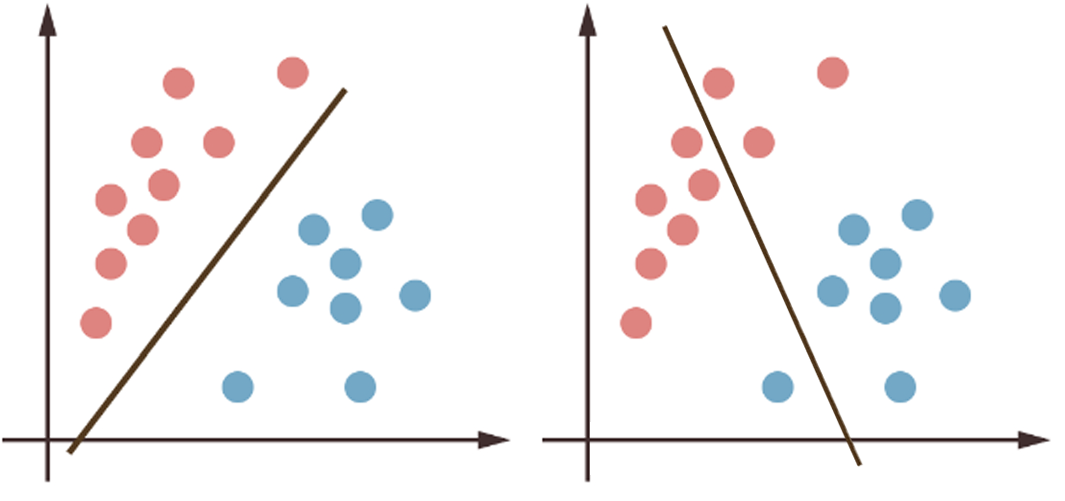
\includegraphics[width=12.4cm]{gbclassified.png}
	\caption{Clasificación de datos linealmente separables en un espacio bidimensional.}
    \label{fig:linsep}
\end{figure}

La Figura \ref{fig:linsep} ilustra dos ejemplos de clasificación de un perceptrón en un espacio de entrada bidimensional ($d=2$). En el dibujo de la izquierda los ejemplos están perfectamente clasificados mientras que en el de la derecha hay algunos ejemplos mal clasificados. Valores diferentes para los parámetros $b,w_1,w_2$ dan lugar a diferentes rectas $w_1x_1+w_2x_2+b=0$. Si el conjunto de datos es linealmente separable existirá una elección de parámetros que clasifica todos los ejemplos correctamente.

\subsection{Ejemplo: Perceptrón} \label{subsec:perceptron}

Introduciremos el algoritmo de del perceptrón como un ejemplo simple de un modelo de aprendizaje. Para simplificar la notación de la fórmula del perceptrón, trataremos el sesgo $b$ como un peso $w_0=b$ y lo añadiremos como una coordenada más al vector de pesos $\nm{w}=(w_0,w_1,\dots,w_d)^T$. Además añadimos una coordenada $x_0=1$ al vector $\nm{x}=(x_0,x_1,\dots,x_d)^T$. Observar que tratamos a $\nm{x}$ y $\nm{w}$ como vectores columna. Formalmente denotaremos el espacio de entrada como: $$\mathcal{X}=\{1\}\times \R^d=\{\nm{x}=(x_0,x_1,\dots,x_d)^T \ : \ x_0=1, \ x_1,\dots,x_d \in \R\}.$$

Denotando $\nm{w}^T\nm{x}=\displaystyle \sum_{i=0}^d w_ix_i$, podemos reescribir la Ecuación \ref{eq:sign-6} como: $$h(\nm{x})=\text{sign}(\nm{w}^T\nm{x}).$$

El algoritmo determinará el valor de $\nm{w}$ basado en los datos. Supondremos que el conjunto de datos es linealmente separable, lo que significa que podemos encontrar un vector $\nm{w}$ tal que $h(\nm{x})$ consigue una decisión correcta $h(\nm{x}_n)=y_n$ para todos los ejemplos del conjunto de datos de entrenamiento.\\

\begin{figure}[h]
	\centering
	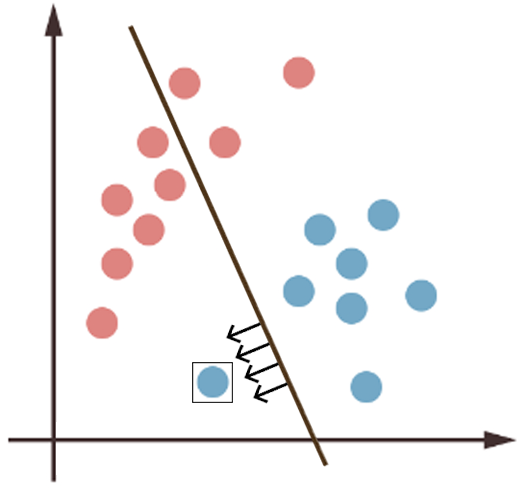
\includegraphics[width=7.8cm]{movclassified.png}
	\caption{Esquema de actualización del algoritmo del perceptrón.}
    \label{fig:movsep}
\end{figure}

Nuestro algoritmo de aprendizaje encontrará este $w$ usando un simple método iterativo, que funciona de la siguiente forma:

En cada paso $t=0,1\dots$, hay un valor actual del vector de pesos $\nm{w}_t$, seleccionamos aleatoriamente un índice $i\in \{1,\dots,n\}$ correspondiente a un ejemplo actualmente mal clasificado, lo denota como $(\nm{x}_t,y_t)$ y lo usa para actualizar el valor de $\nm{w}_t$. Como el ejemplo está mal clasificado, tenemos que $y_t\neq \text{sign}(\nm{w}^T_t\nm{x}_t)$. La regla de actualización viene dada por la siguiente expresión: $$\nm{w}_{t+1}=\nm{w}_t+y_t\nm{x}_t.$$

Esta regla mueve la frontera con el objetivo de cambiar la dirección en la clasificación correcta de $\nm{x}_t$, como se puede ver en la Figura \ref{fig:movsep}. El algoritmo continua con las sucesivas iteraciones hasta que no haya ejemplos mal clasificados en el conjunto de datos.

Aunque la regla de actualización solo considera un único ejemplo del conjunto de entrenamiento y podría desordenar la clasificación para otros ejemplos no implicados en la iteración actual, el algoritmo garantiza una solución óptima (véase Teorema 1 en~\cite{perceptronproof2012}). El resultado se mantiene de forma independiente al ejemplo que elijamos y a la inicialización del vector de pesos al comienzo del algoritmo. Por simplicidad, elegiremos un ejemplo mal clasificado aleatorio e inicializaremos $w_0$ como un vector de ceros.

\subsection*{Otra definición del algoritmo}

Podemos definir el algoritmo de perceptrón como una instancia de la minimización del riesgo empírico (\cite{fairnesslearning2019}). Por la descripción del algoritmo, buscamos un separador lineal y por tanto, nuestro conjunto de hipótesis corresponde con la clase de funciones lineales $$\mathcal H = \{ f(\nm{x}) = \langle \nm{w},\nm{x} \rangle \ : \ \nm{w} \in \mathbb R^d \}.$$

Utilizaremos el método de gradiente estocástico como base del algoritmo, ya que es un método de optimización que elige un ejemplo aleatorio en cada paso y realiza una actualización de los parámetros del modelo. Se define con la regla siguiente: $$\nm{w}_{t+1}=\nm{w}_t-\eta \nabla_{\nm{w}_t} \ell (f(\nm{x}_t),y_t).$$

Donde $\nabla \ell (f(\nm{x}_t),y_t)$ es el gradiente de la función de pérdida con respecto a los parámetros del modelo $\nm{w}_t$ para un ejemplo $(\nm{x}_t,y_t)$. El escalar $\eta > 0$, es un parámetro denominado \textit{tamaño de paso}, normalmente referido a una constante pequeña.

Consideramos ahora la función de pérdida $$\ell(y,\langle \nm{w},\nm{x} \rangle)=\max (1-y\langle \nm{w},\nm{x} \rangle,0),$$

donde su gradiente se define como: $$\nabla \ell (y,\langle \nm{w},\nm{x} \rangle)=\left \{
\begin{array}{l l}
-y\nm{x}, & \mbox{si } y\langle \nm{w},\nm{x} \rangle < 1, \\
0, & \mbox{si } y\langle \nm{w},\nm{x} \rangle > 1.
\end{array}
\right.$$

La expresión anterior define una parte de la regla de actualización del perceptrón, la otra parte la deduciremos al añadir la penalización $\frac{\upalpha}{2}\norm{\nm{w}}^2$ (donde $\norm{\cdot}$ denota la norma euclídea) a la función de pérdida para impedir que los pesos tomen valores por encima de un umbral establecido. Esta penalización se denomina \textit{regularización $\ell_2$} o \textit{regularización de Tíjonov} y su propósito es fomentar la generalización.

Sumando las dos funciones de pérdida, obtenemos una expresión del riesgo empírico regularizado por $\ell_2$ para la función de pérdida de bisagra (\textit{hinge loss}). $$R_{\mathcal{D}}(\nm{w})=\frac{1}{n}\sum_{i=1}^n \max (1-y_i\langle \nm{w},\nm{x}_i \rangle,0)+\frac{\upalpha}{2}\norm{\nm{w}}^2.$$

Definiremos el algoritmo perceptrón como la solución a este problema de minimización del riesgo empírico utilizando el método del gradiente estocástico.

\subsection{Regresión lineal}

Volviendo al ejemplo del apartado \ref{subsec:ejemplobanco}, recordemos que el banco tiene un registro de clientes con variables que pueden ser usadas para aprender un clasificador lineal de decisión para la aprobación del crédito. En este caso, en lugar de limitarnos a tomar una decisión binaria (aprobar o no el crédito), en el caso de aprobación, podríamos querer establecer un umbral en el valor del crédito concedido. Esta tarea, puede ser automatizada haciendo uso del aprendizaje por \textit{regresión} (\cite{learning2012}). 

El banco parte de un conjunto de datos $\mathcal{D}=\{(\nm{x}_1,y_1),\dots,(\nm{x}_n,y_n)\}$, donde $\nm{x}_n$ es la información del cliente e $y_n$ es el límite de crédito establecido por uno de los expertos del banco. Ahora $y_n$ será un número real en lugar de un valor binario. El banco querrá usar un modelo de aprendizaje para encontrar una hipótesis $g$ que replique la actuación humana en el umbral de concesión del crédito. En este caso, no buscaremos una función determinista $y = f(x)$, sino que supondremos que la etiqueta $y_n$ proviene de una distribución $P(y \mid \nm{x})$. No obstante, la naturaleza del problema sigue siendo la misma, tenemos una distribución desconocida $P(\nm{x}, y)$ que genera cada $(\nm{x}_n, y_n)$ y queremos encontrar una hipótesis $g$ que minimice el error entre $g(\nm{x})$ e $y$ con respecto a esa distribución.

\subsection*{Algoritmo de regresión lineal}

El algoritmo se basa en la minimización del riesgo empírico para la pérdida al cuadrado entre $h(\nm{x})$ e $y$. El problema es equivalente a minimizar la siguiente función:
\begin{equation*}
    R_{\mathcal{D}}(h) = \frac{1}{n} \sum_{i=1}^n (h(\nm{x}_i)-y_i)^2.
\end{equation*}

En regresión lineal, $h$ se expresa como combinación lineal de las componentes de $\nm{x}$: 
\begin{equation*}
    h(\nm{x})=\sum_{i=0}^d w_i x_i = \nm{w}^T \nm{x},
\end{equation*}

donde $x_0=1$ y $\nm{x} \in \{1\} \times \R^d$ y $\nm{w} \in \R^{d+1}$. Para el caso lineal se suele definir una matriz de representación para $R_{\mathcal{D}}(h)$. La matriz de datos $X\in \R^{N \times (d+1)}$ tiene como filas los vectores $\nm{x}_n$ e $\nm{y}\in \R^n$ como vector columna cuyas componentes son los valores objetivo $y_n$. Podemos expresar el error en función de $\nm{w}, X$ e $\nm{y}$ como:
\begin{equation}
\begin{split}
    R_{\mathcal{D}}(\nm{w})&=\frac{1}{n}\sum_{i=1}^n (\nm{w}^T\nm{x}_i-y_i)^2\\
    &=\frac{1}{n} \norm{X\nm{w}-\nm{y}}^2\\
    &=\frac{1}{n} (\nm{w}^TX^TX\nm{w} -2\nm{w}^TX^T\nm{y}+\nm{y}^T\nm{y}).
\end{split}
\label{eq:derivable}
\end{equation}

Nuestro problema se reduce a minimizar la función dada por: 
\begin{equation}
    \underset{\nm{w}\in \R^{d+1}}{\text{arg min}} \ R_{\mathcal{D}}(\nm{w}).
    \label{eq:soloptima}
\end{equation}\

\begin{figure}[h]
	\centering
	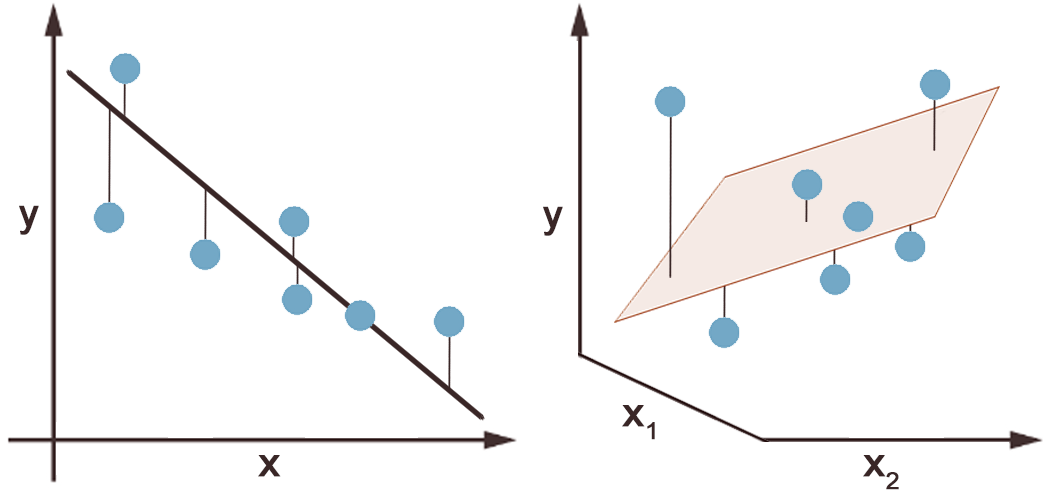
\includegraphics[width=13.3cm]{linear_regresion.png}
	\caption{Problema de regresión lineal en una y dos dimensiones respectivamente.}
    \label{fig:reglin}
\end{figure}

La Figura \ref{fig:reglin} ilustra la solución para los casos unidimensional y bidimensional respectivamente. La Ecuación \ref{eq:derivable} implica que $R_{\mathcal{D}}(\nm{w})$ es diferenciable, por lo que podemos encontrar el mínimo de esta función igualando su gradiente a cero.
\begin{equation*}
    \nabla R_{\mathcal{D}}(\nm{w}) = \frac{2}{n} (X^TX\nm{w}-X^T\nm{y}) = 0.
\end{equation*}

Para encontrar la solución se debe cumplir que $X^TX\nm{w}=X^T\nm{y}$. Si $X^TX$ es regular, $\nm{w}=(X^TX)^{-1}X^T \nm{y}$ es la única solución óptima para la Ecuación \ref{eq:soloptima}. En otro caso, existirá una solución óptima, pero no será única.

\section{Evaluación en aprendizaje automático}

\label{sec:evalaa}

Un modelo en aprendizaje automático funciona bien, cuando puede predecir resultados correctos a partir de un conjunto de datos de entrada no conocido previamente. La manera de medir este fenómeno, no es única, por lo que existen una gran cantidad de \textit{métricas de rendimiento} en el ámbito del \textit{machine learning}. La elección de la métrica dependerá del problema específico, su dominio y de sus restricciones al mundo real. Sin embargo, la mayoría de las métricas se definen como funciones de una \textit{matriz de confusión}. 

Una matriz de confusión define un modelo de predicción a partir de las dimensiones de los \textit{valores reales de las etiquetas} y de sus posibles \textit{predicciones}, resumiendo el número de predicciones correctas e incorrectas por clase.\\

\begin{table}[h]
\centering
\resizebox{9.4cm}{!} {
\begin{tabular}{cc|c|c|}
\cline{3-4}
\multicolumn{1}{l}{}                                                                                      & \multicolumn{1}{l|}{} & \multicolumn{2}{c|}{\textbf{Etiqueta real}}                                                                                          \\ \cline{3-4} 
                                                                                                          &                       & \textbf{$y=1$}                                                     & \textbf{$y=-1$}                                                    \\ \hline
\multicolumn{1}{|c|}{\multirow{2}{*}{\textbf{\begin{tabular}[c]{@{}c@{}}Predicción \end{tabular}}}} & \textbf{$\hat{y}=1$}        & \begin{tabular}[c]{@{}c@{}}Verdadero \\ Positivo (TP)\end{tabular} & \begin{tabular}[c]{@{}c@{}}Falso\\ Positivo (FP) \\ \textcolor{blue}{(Error tipo I)}\end{tabular}     \\ \cline{2-4} 
\multicolumn{1}{|c|}{}                                                                                    & \textbf{$\hat{y}=-1$}        & \begin{tabular}[c]{@{}c@{}}Falso \\ Negativo (FN) \\ \textcolor{blue}{(Error tipo II)}\end{tabular}     & \begin{tabular}[c]{@{}c@{}}Verdadero\\ Negativo (TN)\end{tabular} \\ \hline
\end{tabular}
}
\caption{Matriz de confusión: ilustra la relación entre la etiqueta real y la predicción.}
\label{tab:table2}
\end{table}

Una matriz de confusión binaria como la de la Tabla \ref{tab:table2}, nos ofrece información sobre el número de \textit{verdaderos positivos} (TP) ($y=1 \ \wedge \ \hat{y}=1$), \textit{falsos positivos} (FP) ($y=-1 \ \wedge \ \hat{y}=1$), \textit{falsos negativos} (FN) ($y=1 \ \wedge \ \hat{y}=-1$) y \textit{verdaderos negativos} (TN) ($y=-1 \ \wedge \ \hat{y}=-1$). A partir de ellos, podemos obtener el número total de positivos predichos (TP+FP), el número total de negativos predichos (TN+FN), el número total de etiquetados positivos (TP+FN), y
el número total de etiquetados negativos (TN+FP). 

Además, podemos definir las siguientes métricas de clasificación avanzadas construidas a partir de combinaciones lineales de las básicas:\\

\begin{itemize}
    \item \textbf{Tasa de verdaderos positivos} (\textit{Recall}), $$\text{TPR}=\ddfrac{\text{TP}}{\text{TP+FN}}.$$
    \item \textbf{Tasa de falsos negativos}, $$\text{FNR}=1-\text{TPR}=\ddfrac{\text{FN}}{\text{TP+FN}}.$$
\end{itemize}

\clearpage

\begin{itemize}
    \item \textbf{Tasa de verdaderos negativos} (\textit{Specificity}), $$\text{TNR}=\ddfrac{\text{TN}}{\text{TN+FP}}.$$
    \item \textbf{Tasa de falsos positivos}, $$\text{FPR}=1-\text{TNR}=\ddfrac{\text{FP}}{\text{TN+FP}}.$$
    \item \textbf{Valor positivo predictivo} (\textit{Precision}),  $$\text{PPV}=\ddfrac{\text{TP}}{\text{TP+FP}}.$$
    \item \textbf{Tasa de falso descubrimiento}, $$\text{FDR}=1-\text{PPV}=\ddfrac{\text{FP}}{\text{TP+FP}}.$$
    \item \textbf{Valor negativo predictivo}, $$\text{NPV}=\ddfrac{\text{TN}}{\text{TN+FN}}.$$
    \item \textbf{Tasa de falsa omisión}, $$\text{FOR}=1-\text{NPV}=\ddfrac{\text{FN}}{\text{TN+FN}}.$$
    \item \textbf{Exactitud} (\textit{Accuracy}), $$\text{Accuracy}=\ddfrac{\text{TP+TN}}{\text{TP+TN+FP+FN}}.$$
\end{itemize}\

\begin{table}[h]
\centering
\resizebox{14.1cm}{!} {
\begin{tabular}{cc|c|c|cc}
\cline{3-4}
                                                           &              & \multicolumn{2}{c|}{\textbf{Etiqueta real}}                                                                                                                                 &                                                                                                             &                                                                                                                    \\ \cline{3-4}
                                                           &              & $y=1$                                                                                   & $y=-1$                                                                                  &                                                                                                             &                                                                                                                    \\ \hline
\multicolumn{1}{|c|}{\multirow{2}{*}{\textbf{Predicción}}} & $\hat{y}=1$  & \begin{tabular}[c]{@{}c@{}}Verdadero \\ Positivo (TP)\end{tabular}                      & \begin{tabular}[c]{@{}c@{}}Falso\\ Positivo (FP)\end{tabular}                           & \multicolumn{1}{c|}{\begin{tabular}[c]{@{}c@{}}\textbf{Precision}\\ $\ddfrac{TP}{TP+FP}$\end{tabular}}               & \multicolumn{1}{c|}{\begin{tabular}[c]{@{}c@{}}\textbf{Tasa de Falso}\\ \textbf{Descubrimiento}\\ $\ddfrac{FP}{TP+FP}$\end{tabular}} \\ \cline{2-6} 
\multicolumn{1}{|c|}{}                                     & $\hat{y}=-1$ & \begin{tabular}[c]{@{}c@{}}Falso \\ Negativo (FN)\end{tabular}                          & \begin{tabular}[c]{@{}c@{}}Verdadero\\ Negativo (TN)\end{tabular}                       & \multicolumn{1}{c|}{\begin{tabular}[c]{@{}c@{}}\textbf{Tasa de Falsa}\\ \textbf{Omisión}\\ $\ddfrac{FN}{TN+FN}$\end{tabular}} & \multicolumn{1}{c|}{\begin{tabular}[c]{@{}c@{}}\textbf{Valor Negativo}\\ \textbf{Predictivo}\\ $\ddfrac{TN}{TN+FN}$\end{tabular}}    \\ \hline
                                                           &              & \begin{tabular}[c]{@{}c@{}}\textbf{Recall}\\ $\ddfrac{TP}{TP+FN}$\end{tabular}                   & \begin{tabular}[c]{@{}c@{}}\textbf{Tasa de Falsos}\\ \textbf{Positivos}\\ $\ddfrac{FP}{TN+FP}$\end{tabular} & \multicolumn{1}{c|}{\begin{tabular}[c]{@{}c@{}}\textbf{Accuracy}\\ $\ddfrac{TP+TN}{TP+TN+FP+FN}$\end{tabular}}       &                                                                                                                    \\ \cline{3-5}
                                                           &              & \begin{tabular}[c]{@{}c@{}}\textbf{Tasa de Falsos}\\ \textbf{Negativos}\\ $\ddfrac{FN}{TP+FN}$\end{tabular} & \begin{tabular}[c]{@{}c@{}}\textbf{Specificity}\\ $\ddfrac{TN}{TN+FP}$\end{tabular}              &                                                                                                             &                                                                                                                    \\ \cline{3-4}
\end{tabular}
}
\caption{Matriz de confusión con métricas de evaluación avanzadas.}
\label{tab:tableadv}
\end{table}

\clearpage

Normalmente mediremos el rendimiento de un modelo con una de las métricas mencionadas previamente o, en su defecto, con una combinación de ambas. Una de las medidas de rendimiento más usadas es el \textit{valor positivo predictivo} o \textit{precisión}, que mide el porcentaje de predicciones correctas realizas. Sin embargo, existen problemas derivados de utilizar la precisión a la hora de medir el rendimiento cuando abordamos problemas que contienen desequilibrio entre las clases del conjunto de datos. Por ejemplo, si solo $5$ de cada $100$ muestras es positiva, un modelo trivial que siempre prediga la clase negativa tendrá una precisión del $95\%$.\\

\begin{figure}[h]
	\centering
	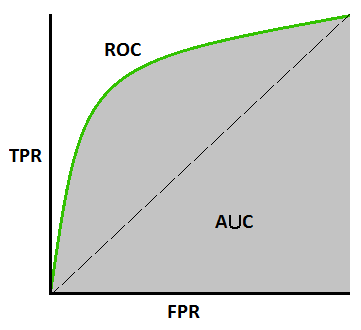
\includegraphics[width=7.8cm]{ROC_curve.png}
	\caption{Ejemplo de un gráfico de curva ROC.}
    \label{fig:curvaROC}
\end{figure}

Otras métricas comúnmente utilizadas son la \textit{F$_1$-score} la cual podemos calcularr como F$_1$-score$=2 \cdot \ddfrac{\text{PPV}\cdot \text{TPR}}{\text{PPV}+\text{TPR}}$ y el \textit{área bajo la curva ROC} (AUC). La curva ROC se representa en
un gráfico bidimensional, en el que la tasa de verdaderos positivos (TPR) se dibuja en el eje vertical y la tasa de falsos positivos (FPR) en el eje horizontal. Como podemos ver en la Figura \ref{fig:curvaROC}, diferentes umbrales de clasificación corresponden a diferentes puntos en el espacio ROC.  

El área bajo la curva ROC (AUC) se interpreta como la probabilidad de que el modelo clasifique más alto un ejemplo positivo aleatorio más que uno negativo también aleatorio. Al ser una probabilidad, el AUC oscilará entre los valores $0$ y $1$. Un modelo cuyas predicciones sean un 100\% incorrectas tendrá un AUC de $0$, mientras que otro cuyas predicciones sean un 100\% correctas tendrá un AUC de $1$. También es importante saber que el AUC es invariable con respecto a la escala y con respecto al umbral de clasificación por lo que es una buena métrica de evaluación para cualquier tipo de problemas en este ámbito.



\chapter{Formalización de las Medidas de equidad} \label{ch:formalmedeq}

En este capítulo presentaremos el concepto de equidad, realizaremos un análisis de las distintas nociones de equidad conocidas y formalizaremos sus definiciones.

\section{¿Qué es la equidad?}

Con el aumento de los métodos de toma de decisiones automatizadas en la actualidad, la necesidad de satisfacer \textit{equidad} en los modelos de \textit{machine learning} ha cobrado importancia. Por ello, cabe hacerse las siguientes preguntas: ¿Qué es la equidad? ¿Cómo podemos medirla? ¿Y, cómo podemos fomentarla en nuestros algoritmos? En esta sección se intentará dar respuesta a estas preguntas.

En la Sección \ref{sec:queaprendizaje}, formalizamos el proceso de aprendizaje automático sobre un ejemplo de aprobación de créditos bancarios. Hemos visto que existe un proceso de apredizaje sobre registros históricos de datos que nos aportan información a la hora de predecir nuevos ejemplos, pero: ¿Existirán atributos que discriminen a un grupo determinado de la población?, ¿Dos clientes con características similares recibirán la misma predicción? Estas preguntas son las motivaron el concepto de equidad.\\

\begin{figure}[h]
	\centering
	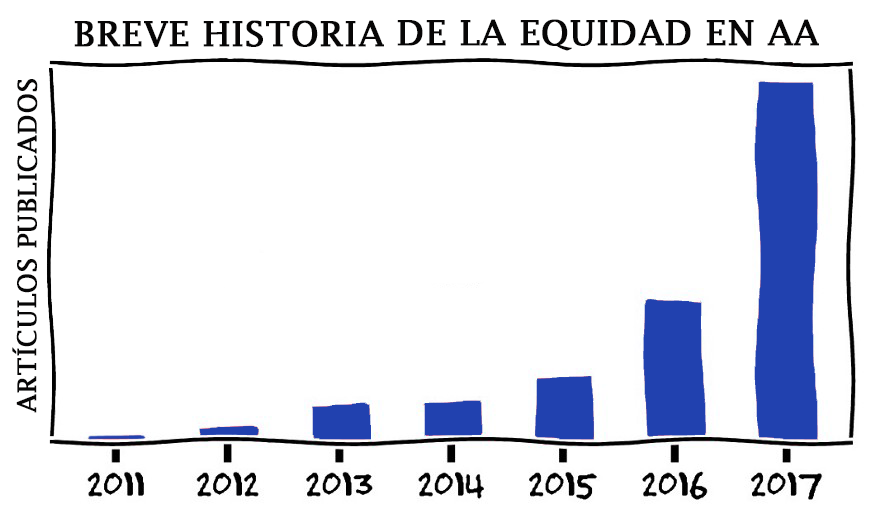
\includegraphics[width=11.05cm]{exponencial.png}
	\caption{Incremento de las publicaciones sobre equidad entre 2011 y 2017.}
\end{figure}

\clearpage

Podemos dividir los trabajos sobre equidad en \textit{machine learning} en, detectar el sesgo y discriminación en los modelos (\cite{detect2012}) y mitigar el sesgo algorítmico (\cite{mitigate2017}). Para estas tareas, al igual que en cualquier ciencia experimental, debemos ser capaces de medir el concepto partiendo de una definición teórica. La equidad es un concepto inherentemente subjetivo y que depende en gran medida del ámbito en el que lo apliquemos. Por lo tanto, a partir de conceptos de la literatura de la ciencias sociales, se han ido proponiendo diferentes medidas y formalizando estos conceptos para que puedan aplicarse al aprendizaje automático.

La primera idea es buscar apoyo legal y comprobar si existe alguna definición que pueda utilizarse para formular la equidad matemáticamente. Existen leyes en la mayoría de países desarrollados, que prohíben el trato desigual entre personas en función de atributos sensibles tales como el sexo o la raza (\cite{ley1964}). Estas leyes suelen evaluar la imparcialidad de un proceso de toma de decisiones utilizando dos nociones distintas (\cite{bigdata2016}): el tratamiento dispar y el impacto dispar. Un proceso de toma de decisiones sufrirá un trato dispar si basamos su juicio en el atributo sensible del sujeto, y tendrá un impacto dispar si sus resultados perjudican (o benefician) de forma desigual a personas con valores de atributos sensibles diferentes.

\subsection{Principales familias de las medidas de equidad}

Los conceptos anteriores son demasiado abstractos como para tener una formulación cuantitativa directa por lo que, poco a poco, se han ido añadiendo numerosas definiciones de equidad a la literatura del aprendizaje automático. Sin embargo, la Tabla \ref{tab:table1} recoge los criterios más importantes, los cuales han sido previamente recopilados en trabajos como \cite{formalizing2018} o \cite{definitions2018}.  

En este capítulo, nos centraremos en las medidas de equidad relativas a \textit{impacto y tratamiento dispar}, estableciendo a su vez una división más específica en algunas de ellas. Los conceptos que trataremos a lo largo de este capítulo son:

\begin{itemize}
    \item \textbf{Equidad por desconocimiento}.
    \item \textbf{Equidad individual}.
    \item \textbf{Equidad de grupo}: formalizaremos la paridad demográfica, el criterio de probabilidades igualadas y la tasa de paridad predictiva.
    \item \textbf{Medidas causales}: analizaremos su base matemática y desarrollaremos un ejemplo práctico de su aplicación en la Parte \ref{part:analisis_exp} de este trabajo. \vspace{2mm}
\end{itemize}

La equidad basada en \textit{preferencias} está fuera del marco de este trabajo, por lo que no será explicada en profundidad. Para el lector interesado en este criterio, puede consultar el artículo \cite{preferences2017}.

\subsection{Medición de la parcialidad y la equidad}

Consideramos una tarea de la clasificación estándar en la que el objetivo es predecir una variable de resultado binaria $y \in \mathcal{Y}$, utilizando un vector de variables de entrada $\nm{x} \in \mathcal{X}$ que sigue una distribución de probabilidad $P_{\nm{x}}$.

Sea un clasificador arbitrario $g:\mathcal{X} \rightarrow \mathcal{Y}$ con $\mathcal{X}=\R^d$, y donde $\mathcal{Y}=[0,1]$ si produce una probabilidad predicha (por ejemplo, regresión logística), o $\mathcal{Y}=\{-1,1\}$ si el clasificador produce un resultado predicho (por ejemplo, SVM). A lo largo del proyecto, normalmente asumiremos que el espacio de salida trabaja sobre decisiones binarias (si/no), es decir, $\mathcal{Y}=\{-1,1\}$.

Muchos de los problemas en los que aparece el concepto de equidad pueden formularse como problemas estadísticos de evaluación de riesgos en los que asignamos una puntuación de valor real $s \in [0,1]$ a cada individuo del conjunto de datos y se toma una decisión $\hat{y}$ basada en la puntuación, normalmente seleccionando un número predefinido de entidades que deben clasificarse como positivas.

Las principales definiciones que usaremos en este capítulo son las siguientes:

\begin{itemize}
    \item \textbf{Vector de características -} $\nm{x}\in \mathcal{X}$ es un vector de características reales que identifican a un individuo.
    \item \textbf{Puntuación -} $s \in [0,1]$ es una puntuación de valor real asignada a cada entidad por el clasificador.
    \item \textbf{Predicción -} $\hat{y} \in \mathcal{Y}$ es una predicción binaria asignada a un individuo determinado, basada en el umbral de la puntuación.
    \item \textbf{Etiqueta real -} $y \in \{-1,1\}$ es la etiqueta binaria que representa el valor real de un individuo en concreto.
\end{itemize}

\section{Equidad por desconocimiento}

\label{sec:eqdesconocimiento}

La \textit{equidad por desconocimiento} se basa en eliminar los atributos sensibles para todos los individuos en el proceso de predicción. Algunos clasificadores propuestos en la literatura de aprendizaje automático satisfacen esta medida (\cite{detect2012}) debido a que es intuitiva y muy fácil de aplicar.

\begin{notation}
Sea $\Delta=\{ \pi(\nm{x})\colon \R^d \to \R^m  \ : \ \nm{x} \in \mathcal{X}, \ 1 \leq m \leq d\}$ el conjunto formado por las proyecciones del conjunto de individuos a todas las posibles dimensiones menores o iguales que la dimensión de $\mathcal{X}$. Sea $\mathcal{A} \subset \Delta$ un subconjunto que contiene todos los individuos de $\mathcal{X}$ a los que se ha aplicado una proyección $\pi$ sobre ciertas características. Notaremos como $\mathcal{A}_i$ al elemento de $\mathcal{A}$ que contiene las características del individuo $\nm{x}_i\in \mathcal{X}$ que cierta proyección $\pi$ ha seleccionado.
\end{notation}\

\begin{definition}[Equidad por desconocimiento]
Sea $\mathcal{A} \subset \Delta$ donde $\mathcal{A}_i$ contiene las proyecciones sobre los atributos sensibles para el individuo $\nm{x}_i$ y sean $g\colon \mathcal{X} \to \mathcal{Y}$ y $h\colon \mathcal{X}\backslash \mathcal{A} \to \mathcal{Y}$ dos clasificadores arbitrarios. Diremos que $g$ logra \textit{equidad por desconocimiento} si, y solo si, 

\begin{equation*} 
g(\nm{x}_i)=h(\nm{x}_i \backslash \mathcal{A}_i), \ \text{para todo} \ \nm{x}_i \in \mathcal{X}.
\end{equation*}
\end{definition}\

Uno de los principales problemas de la equidad por desconocimiento es que no da una condición suficiente para evitar la discriminación, ya que puede haber muchas características altamente correlacionadas (por ejemplo, la zona de residencia) que funcionen como sustitutos del atributo sensible (por ejemplo, la raza). Por lo tanto, no bastaría con eliminar el atributo sensible para eliminar las disparidades. Además, se han documentado diversos ejemplos de equidad por desconocimiento para la raza; en ámbitos como educación, concesión de préstamos o justicia
penal y se ha demostrado que, a largo plazo, el enfoque ciego de la raza es menos eficaz que el enfoque consciente de la misma (\cite{ceguera2008}).

Las críticas anteriores cuestionan la idoneidad de la
equidad por desconocimiento en los dominios en los que, los atributos sensibles pueden deducirse a partir de los atributos no sensibles disponibles, y tenemos conocimiento de la existencia de barreras estructurales, que obstaculizan a los grupos desfavorecidos a partir de encuestas verosímiles sobre los grupos demográficos.

\begin{example} \label{ex:redlining}
Supongamos un modelo utilizado para aprobar o denegar créditos bancarios. Por sesgos históricos, sabemos que uno de los atributos sensibles en la concesión de préstamos, es la raza. Procedemos entonces a eliminar esta información de todos los individuos en el modelo de predicción. El problema surge cuando notamos que el código postal, otro atributo presente en el vector de características, está altamente correlacionado con la raza y por tanto, las decisiones basadas en este serán racialmente discriminatorias. En consecuencia, el criterio de equidad por desconocimiento en este caso concreto, sería insuficiente. 

Esta práctica se conoce como \textit{redlining}, cuyo término fue acuñado en la década de 1960, debido a la práctica de negar bienes y servicios a las minorías mediante la \textit{redlining} de barrios específicos en un mapa (\cite{redlining2012}).
\end{example}


\section{Equidad individual}

La \textit{equidad individual} se basa en métricas de similitud sobre los atributos, y  establece que individuos similares deben recibir predicciones similares independientemente del atributo sensible (\cite{detect2012}). Además, la equidad individual es más precisa que la equidad de grupo, ya que impone restricciones en el tratamiento específico para cada par de individuos.\\ 

\begin{definition}[Equidad individual] \label{def:indvfair}
Sea $g\colon \mathcal{X} \to \mathcal{Y}$ un clasificador arbitrario, $D\colon \mathcal{Y} \times \mathcal{Y} \to \R$ una medida de distancia sobre el espacio de clasificación resultante y $d\colon \mathcal{X} \times \mathcal{X} \to \R$ una medida de distancia sobre los individuos, se dice que $g$ cumple con la \textit{equidad individual} si, y solo si,

\begin{equation*} 
D(g(\nm{x}_i),g(\nm{x}_j))\leq d(\nm{x}_i,\nm{x}_j), \ \text{para todo} \ \nm{x}_i,\nm{x}_j \in \mathcal{X}.
\end{equation*}
\end{definition}\

\begin{figure}[h]
	\centering
	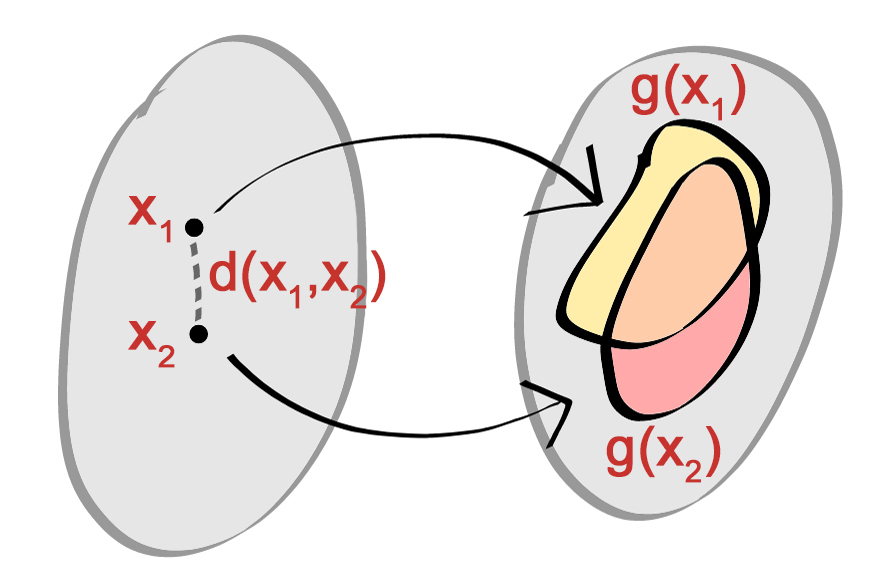
\includegraphics[width=10.5cm]{individual_fair.jpg}
	\caption{Ilustración de la noción de equidad individual.}
    \label{fig:individual_fairness}
\end{figure}

La definición de equidad individual, también es conocida como \textit{propiedad $(D,d)$-Lipschitz}. Cualquier clasificador que satisfaga esta propiedad también verificará la paridad demográfica con un cierto sesgo (véase Lema 3.1 en~\cite{detect2012}).

En la literatura de las ciencias sociales, esta formalización
equivale al individualismo igualitario, conocido por ser el principio formal de justicia. Esta noción responsabiliza a la \textit{métrica de la distancia} de garantizar la justicia del clasificador. Si la métrica de la distancia utiliza los atributos sensibles directa o indirectamente para calcular la distancia entre dos individuos, un clasificador que satisfaga la Definición \ref{def:indvfair} podría seguir causando impacto dispar. Por tanto, la equidad individual, no podría considerarse adecuada para dominios en los que no se dispone de una métrica de distancia fiable y no discriminatoria.

\begin{example}
Imaginemos tres candidatos a un puesto de trabajo, $A$, $B$ y $C$. $A$ tiene únicamente el título de graduado y un año de experiencia laboral relacionada. $B$ tiene un máster y un año de experiencia laboral relacionada. $C$ tiene un doble grado pero no tiene experiencia laboral. En principio, no podemos disponer del rendimiento de los tres individuos ya que no podemos contratar a todos. Entonces: ¿Está $A$ más cerca de $B$ que de $C$? Si es así, ¿Por cuánto? La cosa se complica aún más cuando entran en juego los atributos sensibles. ¿Cómo deberíamos cuantificar la diferencia de pertenencia a un grupo con nuestra métrica?

En este ejemplo podemos observar los problemas de la equidad individual comentados anteriormente, y cómo dependen directamente de la construcción de la función métrica de distancia entre individuos.
\end{example}

\section{Equidad de grupo} 
\label{sec:groupmetrics}

La \textit{equidad de grupo} mide el impacto dispar entre grupos desfavorecidos y privilegiados, como podrían ser grupos de diferentes razas, edad o género.

Supongamos que en $\mathcal{X}$ se definen todas los posibles valores para las características \{raza, género, salario, trabajo, edad\}, denotaremos por $\mathcal{A}$ el conjunto de atributos sensibles sobre $\mathcal{X}$ considerando por ejemplo, en este caso, $$\mathcal{A}\text{=\{raza, género, edad\}}.$$

Consideremos un \textit{atributo multivaluado} $a = \{a_1,\dots,a_n\} \in \mathcal{A}$, por ejemplo, $$\text{raza=\{hispánico, caucásico, afroamericano, otro\}}.$$ Definimos un \textit{grupo} $G(a_i)$
como un conjunto de entidades que tienen en común un valor específico
del atributo $a$, por ejemplo raza=hispánico corresponde a todos los individuos de raza hispánica del
conjunto de datos.

Teniendo en cuenta todos los grupos definidos por el atributo $a$, las predicciones $\hat{y}$ y la etiqueta real $y$ para cada entidad de cada grupo, podemos hablar ahora de las métricas de grupo. Las principales definiciones sobre grupos para evaluar el sesgo y la equidad son las siguientes:

\begin{itemize}
    \item \textbf{Atributo -} $a = \{a_1,\dots,a_n\}$ es un atributo multivaluado, por ejemplo, $$\text{raza=\{hispánico, caucásico, afroamericano, otro\}}.$$
    \item \textbf{Grupo -} $G(a_i)$ es un grupo de todas las entidades que comparten el mismo valor de atributo $a=a_i$, por ejemplo, raza=hispánico.
    \item \textbf{Grupo de objetivo -} $G(a_o)$ es un grupo utilizado como objetivo del cálculo de las métricas de disparidad.
    \item \textbf{Grupo de referencia -} $G(a_r)$ es el grupo que se utiliza como referencia para calcular las métricas de disparidad. Suele fijarse siguiendo un criterio determinado.
    \item \textbf{Etiquetado positivo} - LP$_G$ número de entidades etiquetadas como positivas dentro de un grupo.
    \item \textbf{Etiquetado negativo -} LN$_G$ número de entidades etiquetadas como negativas dentro de un grupo.
\end{itemize}

\clearpage

\begin{notation}
De aquí en adelante, utilizaremos la siguiente notación:

\begin{itemize}
    \item $Y$ es una variable aleatoria binaria, que representa la etiqueta real de un individuo de $\mathcal{X}.$
    \item $\hat{Y}$ es una variable aleatoria binaria, que representa el resultado de la predicción de un clasificador $g\colon \mathcal{X} \to \mathcal{Y}$ para un individuo de $\mathcal{X}.$
    \item $A$ es una variable aleatoria binaria, que representa si un individuo de $\mathcal{X}$ pertenece al grupo objetivo ($a_o$) o de referencia ($a_r$).
\end{itemize}
\end{notation}

\subsection*{Métricas de grupos de distribución}

Concretaremos \textit{métricas de decisión} a nivel de grupo, centradas en la distribución de los individuos entre los grupos del conjunto seleccionado para la intervención, las cuales no precisan del valor de la etiqueta $Y$. Definimos las métricas de distribución de los grupos como sigue:

\begin{itemize}
    \item \textbf{Positivos predichos -} PP$_G$ número de entidades dentro de un grupo donde la decisión es positiva, es decir, $\hat{Y} = 1$.
    \item \textbf{Negativos predichos -} PN$_G$ número de entidades dentro de un grupo cuya decisión es negativa, es decir, $\hat{Y} = -1$.
    \item \textbf{Total de predicciones positivas -} número total de entidades predichas como positivas en los grupos definidos por $a$, $$\text{K} = \sum_{i=1}^{n} \  \text{PP}_{G(a_i)}.$$
    \item \textbf{Prevalencia predicha -} fracción de entidades dentro de un grupo que se predijo como positiva, $$\text{PPRev}_G = \frac{\text{PP}_G}{\abs{G}} = P(\hat{Y}=1 \mid A=a_i).$$
    \item \textbf{Tasa de positivos predichos -} fracción de las entidades predichas como positivas que pertenecen a un determinado grupo, $$\text{PPR}_G = \frac{\text{PP}_G}{\text{K}} = P(A=a_i \mid \hat{Y}=1).$$
\end{itemize}

\subsection*{Métricas de grupo basadas en la etiqueta real}

A continuación, discutiremos diferentes métricas que surgen dependiendo de la coincidencia o no entre los valores de la variable de predicción $\hat{Y}$ y la etiqueta real $Y$. La mayoría de ellas, ya fueron presentadas en la Sección \ref{sec:evalaa}. Las métricas de grupo basadas en los errores y aciertos son las siguientes:

\begin{itemize} 
    \item \textbf{Falso positivo -} FP$_G$ es el número de entidades del grupo con, $$\hat{Y} = 1 \ \wedge \ Y = -1.$$
    \item \textbf{Falso negativo -} FN$_G$ es el número de entidades del grupo con, $$\hat{Y} = -1 \ \wedge \ Y = 1.$$
    \item \textbf{Verdadero positivo -} TP$_G$ es el número de entidades del grupo con, $$\hat{Y} = 1 \ \wedge \ Y = 1.$$
    \item \textbf{Verdadero negativo -} TN$_G$ es el número de entidades del grupo con, $$\hat{Y} = -1 \ \wedge \ Y = -1.$$
    \item \textbf{Prevalencia -}  fracción de entidades dentro de un grupo cuyo resultado verdadero fue positivo, $$\text{Prev}_G= \frac{\text{LP}_G}{\abs{G}}=P(Y=1 \mid A=a_i).$$
    \item \textbf{Tasa de falso descubrimiento -} fracción de falsos positivos de un grupo dentro de los positivos predichos del mismo, $$\text{FDR}_G = \frac{\text{FP}_G}{\text{PP}_G} = P(Y=-1 \mid A=a_i,\hat{Y}=1).$$
    \item \textbf{Tasa de falsa omisión -} fracción de falsos negativos de un grupo dentro de los negativos predichos del mismo, $$\text{FOR}_G = \frac{\text{FN}_G}{\text{PN}_G} = P(Y=1 \mid A=a_i, \hat{Y}=-1).$$
    \item \textbf{Tasa de falsos positivos -} fracción de falsos positivos de un grupo dentro de los negativos etiquetados del mismo, $$\text{FPR}_G = \frac{\text{FP}_G}{\text{LN}_G} = P(\hat{Y}=1 \mid A=a_i,Y=-1).$$
    \item \textbf{Tasa de falsos negativos -} fracción de falsos negativos de un grupo dentro de los positivos etiquetados del mismo, $$\text{FNR}_G = \frac{\text{FN}_G}{\text{LP}_G} = P(\hat{Y}=-1 \mid A=a_i,Y=1).$$
    \item \textbf{Valor negativo predictivo -} fracción de verdaderos negativos de un grupo dentro de los negativos predichos del mismo, $$\text{NPV}_G = \frac{\text{TN}_G}{\text{PN}_G} = P(Y=-1 \mid A=a_i,\hat{Y}=-1).$$
    \item \textbf{Valor positivo predictivo (Precision) -} fracción de verdaderos positivos de un grupo dentro de los positivos predichos del mismo, $$\text{PPV}_G = \frac{\text{TP}_G}{\text{PP}_G} = P(Y=1 \mid A=a_i,\hat{Y}=1).$$
    \item \textbf{Tasa de verdaderos positivos (Recall) -} fracción de verdaderos positivos de un grupo dentro de los positivos etiquetados del mismo, $$\text{TPR}_G = \frac{\text{TP}_G}{\text{LP}_G} = P(\hat{Y}=1 \mid A=a_i,Y=1).$$
    \item \textbf{Tasa de verdaderos negativos (Specificity) -} fracción de verdaderos negativos de un grupo dentro de los negativos etiquetados del mismo, $$\text{TNR}_G = \frac{\text{TN}_G}{\text{LN}_G} = P(\hat{Y}=-1 \mid A=a_i,Y=-1).$$
    \item \textbf{Exactitud (Accuracy) -} fracción de resultados verdaderos de un grupo dentro del total de casos examinados del mismo, $$\text{Accuracy}_G = \frac{\text{TP}_G+\text{TN}_G}{\text{LP}_G+\text{LN}_G} = P(\hat{Y}=Y \mid A=a_i).$$
    \item \textbf{Tasa global de clasificación errónea. -} fracción de resultados falsos de un grupo dentro del total de casos examinados del mismo, $$\text{OMR}_G = \frac{\text{FP}_G+\text{FN}_G}{\text{LP}_G+\text{LN}_G} = P(\hat{Y}\neq Y \mid A=a_i).$$
\end{itemize}\

En los apartados siguientes, formalizaremos algunas de las nociones populares de equidad de grupo que podemos encontrar en la literatura. Sea un atributo sensible multivaluado $a\in \mathcal{A}$, las métricas relativas a equidad de grupo se definen como una igualdad entre las probabilidades de un \textit{grupo objetivo} ($a_o$) en comparación con un \textit{grupo de referencia} ($a_r$).

El grupo de referencia se suele seleccionar en base a diferentes criterios. Por ejemplo, se podría utilizar el grupo mayoritario entre los grupos definidos por $A$, o el enfoque
tradicional de fijar un grupo históricamente favorecido, por ejemplo, en el caso de la raza, los individuos de raza caucásica.


\subsection{Paridad demográfica}

La \textit{paridad demográfica}, también conocida como \textit{paridad estadística} o \textit{independencia}, es uno de los criterios de equidad de grupo más conocidos. Esta noción de equidad afirma que la probabilidad de ser clasificado con el resultado positivo (o negativo) debe ser independiente de que el individuo pertenezca al grupo protegido, es decir, que los datos demográficos de los individuos clasificados positivamente son idénticos a los de la población en su conjunto (\cite{detect2012}).\\

\begin{definition}[Independencia en clasificación binaria]
Sean $C,A$ variables aleatorias. La \textit{independencia} entre $C$ y $A$, equivale a que se cumpla la siguiente restricción:
$$P(C=c \mid A=a_r)=P(C=c \mid A=a_o).$$
Lo denotaremos como $C \perp A.$
\end{definition}\

\begin{definition}[Paridad demográfica] \label{def:pardemo}
Sea $A \in \mathcal{A}$ un atributo sensible multivaluado y $g\colon \mathcal{X} \to \mathcal{Y}$ un clasificador arbitrario. Se dice que $g$ cumple con la \textit{paridad demográfica} si, y solo si, $\hat{Y} \perp A.$
\end{definition}

\subsection*{Relajaciones y aproximaciones}

Podemos \textit{relajar} el concepto de paridad demográfica suponiendo que $\hat{Y}=1$ y aproximando su definición con una acotación en valor absoluto de las probabilidades a partir una constante fijada $\tau \in [0,1]$. De esta manera, aproximamos este criterio de equidad como: 
\begin{equation*}
\abs{P(\hat{Y}=1 \mid A=a_r)-P(\hat{Y}=1 \mid A=a_o)} \leq \tau.
\end{equation*}

Tomando un $\epsilon \in [0,1)$ también podemos aproximar el concepto de paridad demográfica de la siguiente manera:
\begin{equation*}\label{eq:p}
   1-\epsilon \leq \ddfrac{P(\hat{Y}=1 \mid A=a_o)}{P(\hat{Y}=1 \mid A=a_r)}. 
\end{equation*}

En algunos trabajos se suele obviar la acotación por una constante y simplemente se define la paridad demográfica utilizando la Definición \ref{def:pardemo} y asumiendo que $\hat{Y}=1$, lo que sería equivalente a igualar las métricas PPRev entre los subgrupos.

\begin{equation*}
\text{PPRev}_{a_r}=\text{PPRev}_{a_o} \Rightarrow P(\hat{Y}=1 \mid A=a_r)=P(\hat{Y}=1 \mid A=a_o).
\end{equation*}

\begin{example}
Consideremos un sistema de detección de delitos y dos grupos de igual tamaño, $A$ y $B$. Suponemos que los miembros del grupo $B$ tienen el doble probabilidades reales de cometer un delito que los individuos del grupo $A$. Al igualar la probabilidad de un resultado positivo, el mismo número de predicciones positivas se distribuiría entre un grupo mucho mayor de delincuentes para $B$ que para $A$. Así, un delincuente del grupo $B$ tendría menos probabilidades de serlo que un delincuente del grupo $A$ ($\text{FNR}_A < \text{FNR}_B$). De hecho, para la misma precisión, la tasa de verdaderos positivos del grupo $B$ sería la mitad de la del grupo $A$, $\frac{1}{2} \text{TPR}_A = \text{TPR}_B$, cumpliendo la paridad demográfica.
\end{example}

\subsection{Probabilidades igualadas}

Uno de los problemas de la paridad demográfica es que ignora una posible correlación entre $Y$ y $A$. El criterio de las \textit{probabilidades igualadas}, también conocido como \textit{ratio de paridad positiva} o \textit{separación}, tiene en cuenta la etiqueta real de cada grupo y su condicionamiento al resto de variables. Además, proporciona un incentivo para reducir los errores de manera uniforme en todos los grupos sin descartar el clasificador perfecto (que obtenga $\hat{Y}=Y$) a diferencia de la paridad estadística.\\

\begin{definition}[Independencia condicional en clasificación binaria]
Sean $C,Y,A$ variables aleatorias. La \textit{independencia condicional} entre $C$ y $A$ dado $Y$, equivale a que se cumpla la siguiente restricción:
$$P(C=c \mid A=a_r, Y=y)=P(C=c \mid A=a_o,Y=y).$$
Lo denotaremos como $C \perp A \mid Y.$
\end{definition}\

El criterio de las probabilidades igualadas establece que $\hat{Y}$ debe ser condicionalmente independiente de $A$ dado $Y$, permitiendo que el clasificador dependa de $A$ a través de la variable objetivo (\cite{eodd2016}). Para utilizar este criterio, es necesario conocer las etiquetas reales de cada individuo, por lo que esta medida restringe su uso para determinadas tareas en las que no conozcamos previamente el resultado de la acción sobre el individuo.\\

\begin{definition}[Probabilidades igualadas] \label{def:probigual}
Sea $A \in \mathcal{A}$ un atributo sensible multivaluado y $g\colon \mathcal{X} \to \mathcal{Y}$ un clasificador arbitrario. Se dice que $g$ cumple con el criterio de las \textit{probabilidades igualadas} si, y solo si, $\hat{Y} \perp A \mid Y$.
\end{definition}

\subsection*{Relajaciones y aproximaciones}

El concepto previo depende de varias variables, por lo que normalmente en la práctica, se tiende a relajar el criterio fijando algunos valores en la definición. A partir de estas relajaciones surgen otros criterios de equidad que también son ampliamente utilizados y conocidos en la literatura.

La relajación más común surge al suponer que $\hat{Y}=1$, en este caso, el criterio de las probabilidades igualadas equivale a igualar las métricas FPR y TPR entre los subgrupos. Esta aproximación beneficia al individuo, y equilibra la probabilidad de tener un resultado beneficioso, en todos los subgrupos de los individuos etiquetados tanto positiva como negativamente.
\begin{equation*}
\begin{split}
\text{FPR}_{a_r}=\text{FPR}_{a_o} &\Rightarrow P(\hat{Y}=1 \mid A=a_r,Y=-1)=P(\hat{Y}=1 \mid A=a_o, Y=-1).\\
\text{TPR}_{a_r}=\text{TPR}_{a_o} &\Rightarrow P(\hat{Y}=1 \mid A=a_r, Y=1)=P(\hat{Y}=1 \mid A=a_o, Y=1).
\end{split}
\end{equation*}

Definiremos el concepto de igualdad de oportunidades como la igualdad de las tasas de verdaderos positivos entre los subgrupos (\cite{eodd2016}). En algunos trabajos, también se define este criterio de forma equivalente para las tasas de verdaderos negativos.
\begin{equation*}
\text{TPR}_{a_r}=\text{TPR}_{a_o} \Rightarrow P(\hat{Y}= 1 \mid A=a_r, Y=1)=P(\hat{Y}= 1 \mid A=a_o, Y=1).
\end{equation*}\

\begin{definition}[Igualdad de oportunidades]
Sea $A \in \mathcal{A}$ un atributo sensible multivaluado y $g\colon \mathcal{X} \to \mathcal{Y}$ un clasificador arbitrario. Se dice que $g$ cumple con la \textit{igualdad de oportunidades} si, y solo si, $$P(\hat{Y}=1 \mid A=a_r,Y=1)=P(\hat{Y}=1 \mid A=a_o, Y=1).$$
\end{definition}\

La igualdad de oportunidades es naturalmente más débil que la Definición \ref{def:probigual}, ya que asumimos los valores de $\hat{Y}=1$ e $Y=1$. Este concepto, iguala la probabilidad de que los individuos etiquetados positivamente
sean correctamente clasificados con el resultado positivo (beneficioso). Por ejemplo, dos individuos, un
hombre y una mujer, que están cualificados para un trabajo ($Y=1$), deberían tener la misma probabilidad de conseguir el trabajo ($\hat{Y}=1$).

\begin{example}
Consideremos un sistema de contratación y dos grupos de igual tamaño, $A$ y $B$. Imaginemos que en el grupo $A$ de los 100 aspirantes al cargo, 58 están cualificados, mientras que el grupo $B$ solo 2 de ellos son aptos para el cargo. Si la empresa decide aceptar a 30 solicitantes y satisfacer la igualdad de oportunidades, se concederán 29 ofertas al grupo $A$ mientras que solo se concederá 1 oferta al grupo $B$. Si el trabajo es bien remunerado, el grupo $A$ mejorará sus condiciones de vida y a la larga, podrá permitir una mejor educación para sus hijos, y en consecuencia una mejor cualificación de los mismos en el futuro. 

En este ejemplo podemos observar que la igualdad de oportunidades no ayuda a cerrar la brecha entre los dos grupos, es más la brecha entre el grupo $A$ y el grupo $B$, tenderá a ampliarse con el tiempo. 
\end{example}

\subsection{Tasa de paridad predictiva} \label{subsec:suficiencia}

La \textit{tasa de paridad predictiva}, también denominada \textit{suficiencia} surge de una motivación equivalente a la del criterio de las probabilidades igualadas. El concepto se define de igual manera haciendo uso de la independencia condicional, pero intercambiando los papeles de $\hat{Y}$ e $Y$. \\

\begin{definition}[Tasa de paridad predictiva]
Sea $A \in \mathcal{A}$ un atributo sensible multivaluado y $g\colon \mathcal{X} \to \mathcal{Y}$ un clasificador arbitrario. Se dice que $g$ cumple con la \textit{tasa de paridad predictiva} si, y solo si, $Y \perp A \mid \hat{Y}$.
\end{definition}

\subsection*{Relajaciones y aproximaciones}

La relajación más común surge al suponer que $\hat{Y}=Y$, en este caso, el criterio de las probabilidades igualadas equivale a igualar las métricas PPV y NPV entre los subgrupos. 
\begin{equation*}
\begin{split}
\text{PPV}_{a_r}=\text{PPV}_{a_o} &\Rightarrow P(Y=1 \mid A=a_r, \hat{Y}=1)=P(Y=1 \mid A=a_o, \hat{Y}=1).\\
\text{NPV}_{a_r}=\text{NPV}_{a_o} &\Rightarrow P(Y=-1 \mid A=a_r,\hat{Y}=-1)=P(Y=-1 \mid A=a_o,\hat{Y}=-1).
\end{split}
\end{equation*}

Las limitaciones de este concepto de equidad son semejantes a las de las probabilidades igualadas, pudiendo acrecentar las diferencias entre los grupos privilegiado y desfavorecido.

\subsection{Medidas basadas en la puntuación}

A diferencia de las definiciones anteriores, que se basan en los índices de clasificación binaria, algunas nociones de equidad se basan en la \textit{puntuación} de la probabilidad predicha $S$ y la etiqueta real $Y$ (\cite{catalogue2018}).

El \textit{balance para la clase positiva} (o \textit{negativa}) se cumple cuando la puntuación esperada para un individuo clasificado positivamente (o negativamente) es igual en todos los grupos.\\

\begin{definition}[Balance para la clase positiva]
Sea $A \in \mathcal{A}$ un atributo sensible multivaluado y $S\in [0,1]$ la puntuación asignada por el clasificador arbitrario $g\colon \mathcal{X} \to \mathcal{Y}$. Se dice que $g$ cumple con el \textit{balance para la clase positiva} si, y solo si, $$\mathbb{E}[S=s \mid A=a_r,Y=1]=\mathbb{E}[S=s \mid A=a_o,Y=1].$$
\end{definition}\

\begin{definition}[Balance para la clase negativa]
Sea $A \in \mathcal{A}$ un atributo sensible multivaluado y $S\in [0,1]$ la puntuación asignada por el clasificador arbitrario $g\colon \mathcal{X} \to \mathcal{Y}$. Se dice que $g$ cumple con el \textit{balance para la clase negativa} si, y solo si, $$\mathbb{E}[S=s \mid A=a_r, Y=-1]=\mathbb{E}[S=s \mid A=a_o, Y=-1].$$
\end{definition}\

Sin embargo, hay que tener en cuenta que
en los problemas del mundo real es casi imposible cumplir el equilibrio para la clase negativa y para la clase positiva simultáneamente.

\clearpage

\subsection{Igualdad de las métricas de predicción}

Como hemos podido observar, en general, la mayoría de los criterios de equidad definidos surgen como una igualación de las métricas de grupo presentadas al inicio de la Sección \ref{sec:groupmetrics}. De esta forma podemos definir, un nuevo criterio para cada métrica de la siguiente forma.\\

\begin{definition}[Paridad métrica]\label{def:parmetr}
Sea $A \in \mathcal{A}$ un atributo sensible multivaluado y $g\colon \mathcal{X} \to \mathcal{Y}$ un clasificador arbitrario. Se dice que $g$ cumple con la \textit{paridad métrica} si, y solo si, $$\text{Métrica}_{a_r}=\text{Métrica}_{a_o}.$$
Donde Métrica podrá ser cualquier métrica de grupo definida previamente. 
\end{definition}\

Aunque esta definición nos permite crear una gran variedad de criterios de equidad, la formulación a partir de una igualdad sigue siendo difícil a la hora de aplicarla en la práctica. 

\subsection{Impacto desigual} \label{subsec:impactdesi}

Para facilitar la implementación práctica de las métricas anteriores, aparece el término \textit{impacto desigual} (no confundir con el término impacto dispar definido en la Tabla \ref{tab:table1}). Esta noción está directamente relacionada con la regla $p\%$, que podemos encontrar en la literatura jurídica (\cite{prule2018}), según la cual una decisión es discriminatoria si el coeficiente del impacto desigual es inferior a un valor $\tau$ dependiente de $p$ ($\tau=\frac{p}{100}$).\\

\begin{definition}(Impacto desigual) \label{def:mdi}
Sea $A \in \mathcal{A}$ un atributo sensible multivaluado, $g\colon \mathcal{X} \to \mathcal{Y}$ un clasificador arbitrario y $\tau\in [0,1]$. Se dice que $g$ satisface el \textit{impacto desigual} si, y solo si,
\begin{equation} \label{eq:1p}
    DI = \ddfrac{P(\hat{Y}=1 \mid A=a_o)}{P(\hat{Y}=1 \mid A=a_r)} < \tau.
\end{equation}
\end{definition}\

En el mundo real, si un clasificador aplicado a una tarea en una empresa satisface el impacto desigual, debe justificarse que su aplicación es esencial para el funcionamiento seguro y eficiente del negocio, y no existen procedimientos alternativos que sean sustancialmente igual de válidos y tengan un impacto menos adverso. La Comisión para la Igualdad de Oportunidades en el Empleo (EEOC) de Estados Unidos adopta la regla del $80\%$ ($\tau = 0.8$) para considerar si una decisión tiene impacto desigual (\cite{adverse2009}).

\subsection*{Construcción de otras medidas en la práctica}

Si queremos evitar el impacto desigual, impondremos la desigualdad opuesta de la Ecuación (\ref{eq:1p}). Estableciendo además una cota superior dada por $\frac{1}{\tau}$, obtenemos el criterio de equidad implementado por Aequitas (\cite{aequitas2019}). 

\begin{equation*}
\tau \leq \ddfrac{P(\hat{Y}=1 \mid A=a_o)}{P(\hat{Y}=1 \mid A=a_r)} \leq \frac{1}{\tau}.
\end{equation*}

La formulación aportada por Aequitas se basa en calcular la fracción de la métrica de grupo elegida y una vez calculada, comprobar si se encuentra dentro del rango definido. La pertenencia o no al rango será una aproximación a la igualación de las métricas de la Definición \ref{def:parmetr}.

\begin{equation*}
\tau \leq \text{Métrica de disparidad}_{G} \leq \frac{1}{\tau}.
\end{equation*}

Usamos $\tau \in
(0,1]$ para controlar el rango de valores de disparidad que pueden considerarse justos. Para aplicar la regla del 80\%, simplemente bastaría con tomar $\tau=0.8$. Diremos que un clasificador será tan justo como lo permita el valor máximo del sesgo entre los grupos definidos por los atributos protegidos. 

Esta formalización también puede extenderse a cualquier métrica de grupo de las explicadas en la Sección \ref{sec:groupmetrics}. Definiremos, por ejemplo, la tasa de falsas omisiones (FOR) como:

\begin{equation*} 
\text{Métrica FOR}_{G(a_o)} =\frac{\text{FOR}{a_o}}{\text{FOR}{a_r}}=\frac{P(Y=1 \mid A=a_o, \hat{Y}=-1)}{P(Y=1 \mid A=a_r, \hat{Y}=-1)}.
\end{equation*}

Aequitas utiliza la tasa de positivos predichos (PPR) para aproximar el concepto de paridad demográfica. Usaremos unas métricas u otras en función del impacto y el objetivo que quiera intervenir el usuario. Si las intervenciones pueden perjudicar a los individuos (punitivas), entonces querremos minimizar los falsos positivos, centrándonos en la tasa de falsos descubrimientos (FDR) o la de falsos positivos (FPR). Si por otro lado tienen como objetivo beneficiar a los individuos (asistenciales), deberíamos preocuparnos más por los falsos negativos, priorizando la tasa de falsa omisión (FOR) o la de falsos negativos (FNR).

\chapter{Algoritmos de mitigación de sesgo} \label{ch:algmitigar}

En este capítulo discutiremos los diferentes algoritmos existentes para la mitigación del sesgo, daremos algunos ejemplos específicos de los aportados en la bibliografía y comentaremos sus características más relevantes.

\section{Modelos de aprendizaje justos}

En la literatura, podemos encontrar una gran variedad de métodos y algoritmos que nos pueden ayudar a mejorar la equidad en un modelo de aprendizaje. Los enfoques de \textit{mitigación del sesgo} pueden subdividirse en tres categorías: algoritmos de preprocesamiento, que intentan aprender representaciones justas de los datos; algoritmos de optimización durante el entrenamiento, que ajustan el proceso de aprendizaje para cumplir los criterios de justicia; y algoritmos de posprocesamiento, que adaptan las predicciones del modelo en función de sus resultados. Estas categorías no tienen por qué ser mutuamente excluyentes y a veces pueden tener varios métodos de actuación sobre los datos.

A lo largo de este capítulo, presentaremos las características comunes entre los algoritmos de cada uno de los tres grupos presentados y discutiremos algunos ejemplos que podemos encontrar en la literatura, profundizando en algún caso específico de cada tipo. Además, contextualizaremos en su categoría correspondiente el algoritmo de optimización de equidad contrafactual presentado por \cite{counterfactual2018} sobre el que basaremos la parte experimental de nuestro trabajo.

\subsection{Selección de los datos del modelo}

En la Sección \ref{sec:queaprendizaje}, observamos que para construir un modelo de aprendizaje es necesario tener un conjunto de datos $\mathcal{D}=\{(\nm{x}_1,y_1),\dots,(\nm{x}_n,y_n)\}$ a partir del cual poder entrenar el modelo y extraer la información que se quiere aprender. Normalmente para entrenar los modelos, no utilizaremos el conjunto de datos al completo, sino que tomaremos un conjunto de entrenamiento $X$, que contiene $m$  individuos extraídos aleatoriamente del conjunto de datos total, donde $m < n$. Cada elemento $\nm{x} \in X$ es un vector de longitud $d$ donde cada componente del vector describe una característica del individuo. Además, cada vector $\nm{x}$ tiene asociado un atributo sensible $a\in \{0,1\}$, donde el valor $0$ denota la pertenencia al grupo de referencia $(a_r)$ y $1$ al grupo objetivo $(a_o)$. Denotaremos por $Y$ al conjunto con las etiquetas reales de los individuos que están en $X$. De esta forma, tenemos que $X \times Y \subset \mathcal{D}$. 

En la práctica, se suele utilizar el conjunto de los individuos restantes contenidos en $\mathcal{D}$ como conjunto de prueba del modelo, con el objetivo de poder comprobar su rendimiento sobre un conjunto de datos con el que no ha sido entrenado. 

\subsection{Equilibrio entre equidad y métricas de evaluación}

Algunas medidas de evaluación como la precisión o exactitud dependen directamente del conjunto de datos, la definición de equidad utilizada y los algoritmos empleados. La equidad en la práctica, perjudica a métricas como la exactitud. Si queremos mitigar el sesgo entre grupos, debemos hacer una compensación entre la equidad y la exactitud, sacrificando esta última como se puede observar en la Figura \ref{fig:tradeoff}.\\

\begin{figure}[h]
	\centering
	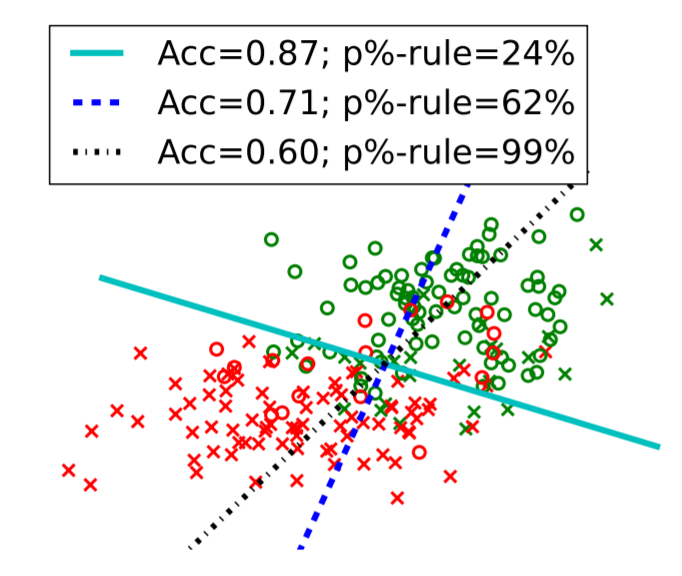
\includegraphics[width=7.6cm]{accuracyeq.png}
	\caption{Exactitud vs. Independencia en un problema de clasificación (\cite{constraints2017}).}
    \label{fig:tradeoff}
\end{figure}

\section{Algoritmos de preprocesamiento}

Los \textit{algoritmos de preprocesamiento} buscan mejorar la equidad antes de entrenar el modelo, modificando los datos de entrenamiento de forma que no presenten sesgos antes de ser procesados. El propósito de estos algoritmos es aprender una nueva representación $Z$ que elimine la información correlacionada con el atributo sensible $A$ y preserve, en la medida de lo posible, la información del conjunto de individuos $X$ sin necesidad de conocer el valor de sus etiquetas $Y$. La tarea posterior (por ejemplo, regresión o clasificación) desempeñada por $g$, será independiente del método usado y podrá producir resultados que preserven diversos criterios de equidad.\\

\begin{figure}[h]
	\centering
	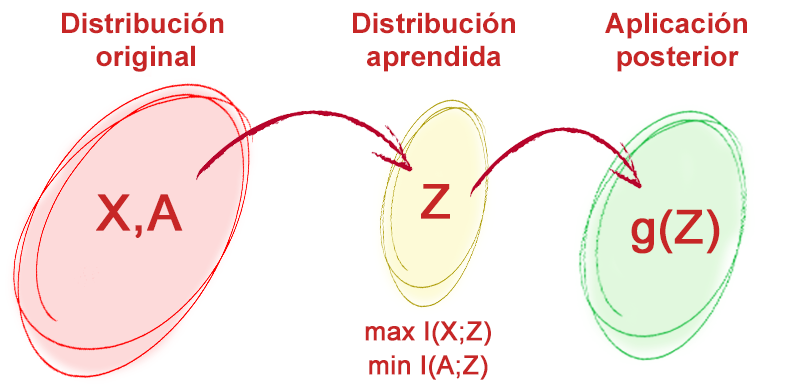
\includegraphics[width=12.1cm]{preprocesado.png}
	\caption{Etapas del proceso de preprocesamiento.}
    \label{fig:preprocessing}
\end{figure}

\subsection{Ejemplo: Aprendizaje de la representación justa}

\cite{fairrepresentation2013} presenta  este problema como el aprendizaje de un función que lleva muestras individuales a representaciones intermedias. Este trabajo tiene dos objetivos: minimizar la pérdida de información (los datos originales deberían preservar la misma cantidad de información) y maximizar la equidad (la pertenencia a un grupo protegido no debería afectar negativamente a los individuos del mismo). 

Este ejemplo, podría confundirse como una aplicación de equidad por desconocimiento, pero no es así, ya que la pertenencia a grupos protegidos no es simplemente ignorada, sino que se trata activamente junto con la información redundante de estos atributos. El modelo propuesto, tiene como objetivo mantener la equidad de grupo e individual, al mismo tiempo que maximiza la exactitud.

\begin{notation}
Introducimos la siguiente notación que utilizaremos en este ejemplo:

\begin{itemize}
    %\item $S$ es una variable aleatoria binaria que representa si un individuo determinado es o no miembro del conjunto protegido. 
    %\item $Y$ es una variable aleatoria binaria que representa la decisión de clasificación de un individuo y $f\colon X \to Y$ es la función de clasificiación.
    \item $X^+=\{\nm{x}_n \in X \ : \ A=1\}\subset X$ es el conjunto de datos de entrenamiento cuyos miembros pertenecen al grupo protegido, $X^-=\{\nm{x}_n \in X \ : \ A=0\}$ denota al conjunto cuyos miembros pertenecen al grupo no protegido.
    \item $Z$ es una variable aleatoria multivariante, donde cada uno de sus $r$ valores representa un ''prototipo''. Asociado a cada prototipo existe un vector $\nm{v}_k$ en el mismo espacio que los individuos $\nm{x}_n$.
\end{itemize}
\end{notation}

La idea es representar cada individuo $\nm{x}_n \in X$ como una combinación lineal ponderada de $r$ prototipos para satisfacer la paridad demográfica, minimizando la pérdida de información original y maximizando la exactitud en la medida de lo posible.

Se define la probabilidad \textit{softmax} de que un elemento sea un prototipo concreto como:
\begin{equation*}
M_{n,k}:= P(Z=k \mid \nm{x}_n)=\ddfrac{\text{exp}(-d(\nm{x}_n,\nm{v}_k))}{\sum_{j=1}^r \text{exp}(-d(\nm{x}_n,\nm{v}_j))}, \ \text{para todo} \ n,k.
\end{equation*}

donde $d$ es una función de medida de distancia (por ejemplo, la distancia $\ell_2$). Los autores definen la regularización $\ell_2$ como una función de distancia ponderada que viene dada por,
\begin{equation*}
d(\nm{x}_n,\nm{v}_k,\upalpha)=\sum_{i=1}^d \upalpha_i (x_{ni}-v_{ki})^2.
\end{equation*}

Se define $\hat{y}_n$ como la predicción para $y_n$ calculada partiendo de la marginalización sobre el valor de $Y$ para la predicción de cada prototipo.
\begin{equation*}
\hat{y}_n=\sum_{k=1}^r M_{n,k} w_k.
\end{equation*}

El modelo de aprendizaje, minimiza la siguiente función de pérdida:
\begin{equation*}
L=A_zL_z+A_xL_x+A_yL_y.   
\end{equation*}

Donde $L_z$ regulariza la paridad demográfica, $L_x$ es el error de reconstrucción de la distribución y $L_y$ cuantifica la pérdida de predicción. Los factores $A_z, A_x, A_y$ se definen como hiperparámetros para equilibrar estas pérdidas.

\begin{equation*}
L_z=\sum_{k=1}^r \abs{M_k^+-M_k^-}.
\end{equation*}
expresando $\displaystyle M_k^+=\frac{1}{\abs{X^+}} \sum_{n\in X^+} M_{n,k}$ y $M_k^-$ se formula de forma similar a partir de $X^-$.

\begin{equation*}
L_x=\sum_{n=1}^m (\nm{x}_n-\hat{\nm{x}}_n)^2.
\end{equation*}
donde $\hat{\nm{x}}_n$ son los nuevos valores de $\nm{x}_n$ para $Z$:
\begin{equation*}
\hat{\nm{x}}_n=\sum_{k=1}^r M_{n,k}\nm{v}_k.
\end{equation*}

\begin{equation*}
L_y=\sum_{n=1}^m -y_n \log \hat{y}_n -(1-y_n) \log (1-\hat{y}_n).
\end{equation*}

En la fase de entrenamiento, los valores de $\nm{v}, \nm{w}, \upalpha$ se optimizan conjuntamente a través del método L-BFGS (\cite{lbfgs1997}), para minimizar la función objetivo $L$. Los valores de $A_x,A_y,A_z$ se seleccionan a través de la afinación de los hiperparámetros, optando por los que producen mejores resultados (búsqueda en malla). Tenemos que tener en cuenta que la función objetivo no es convexa y, por tanto, no garantiza la optimización.

\subsection*{Ventajas e inconvenientes}

Algunas de las principales ventajas de los algoritmos de preprocesamiento, ya han sido mencionadas previamente. En general, estos métodos, son muy útiles cuando el clasificador que utilizaremos para la fase de entrenamiento es un modelo de caja negra y no conocemos su actuación sobre los datos. En estos casos, al devolver una nueva distribución que no contiene correlación con los atributos sensibles, los datos podrán ser usados de forma independiente para cualquier tarea posterior sin preocuparnos por la existencia de sesgo entre grupos.

Por otro lado, solo podemos utilizar los métodos de preprocesamiento para optimizar los criterios de equidad que no requieran información sobre el valor de las etiquetas $Y$ (por ejemplo, la paridad demográfica o la equidad individual). Como desconocemos el uso que se le va a dar a los nuevos datos, en algunos casos, podría no garantizarse la equidad en el modelo final aprendido. Además, este grupo de algoritmos suele ser el peor en términos de rendimiento entre exactitud y equidad.


\subsection*{Otros ejemplos en la literatura}

El concepto de preprocesamiento optimizado es introducido por \cite{optimizeddata2017}. En este se plantea la reducción de la discriminación como una tarea de optimización convexa con el objetivo de minimizar la pérdida de exactitud (preservando la utilidad), mientras se limita por ciertas medidas de equidad de grupo e individual.

\cite{repairing2019} ofrece métodos que usan distribuciones contrafactuales para resolver el trato dispar de un clasificador de caja negra en una población de despliegue sin la necesidad de reentrenar el modelo. El método propuesto se basa en la construcción de una nueva distribución para los individuos del grupo objetivo, de manera que mejoren sus resultados en promedio.

\section{Algoritmos de optimización durante el entrenamiento}

Los \textit{algoritmos de optimización} alteran el entrenamiento del propio modelo. En este contexto, la mitigación del sesgo se plantea como un aprendizaje al que se le añade una restricción o un término de regularización al objetivo de optimización existente. Es decir, un modelo aprende a optimizar una función de pérdida en los datos de entrenamiento, sujeta a restricciones de equidad (por ejemplo, la distancia máxima a la paridad demográfica).

Otro enfoque diferente, sería el de la optimización de métricas de rendimiento complejas que incluyan alguna noción de equidad. Por ejemplo, introduciendo una penalización relacionada con la equidad en la función objetivo.

\subsection{Ejemplo: Aprendizaje en clasificación sin impacto dispar.}

Uno de los enfoques más populares es el de la optimización con restricciones; donde el objetivo es encontrar un conjunto de parámetros $\btheta \in \Theta$, que minimicen una función objetivo $l_0(\btheta)$, sujeta a $m$ restricciones funcionales $l_i(\btheta), \ \text{para todo} \ i \in \{1,\dots,m\}$. $$\btheta^\ast = \underset{\btheta \in \Theta}{\text{arg min}}  \ l_0(\btheta) \ \ \text{donde} \ l_i(\btheta) \leq 0 \ \ \text{para todo} \ i \in \{1,\dots,m\}.$$

\cite{constraints2017} enmarca la tarea de clasificación justa, imponiendo restricciones lineales a la covarianza entre los atributos sensibles y las predicciones. Este método es adecuado para múltiples atributos sensibles y para cualquier clasificador basado en contornos convexos (por ejemplo, SVM o regresión logística). Además, se propone otra formulación similar destinada a satisfacer necesidades del mundo real, maximizando la equidad sujeta a restricciones de exactitud. 

En el trabajo anterior se asume que el conjunto de datos original presenta un sesgo histórico, por lo que en \cite{disparate2017}, se amplía este enfoque a los casos en los que tenemos acceso a los resultados reales no sesgados durante la fase de entrenamiento, y podemos saber si una decisión histórica fue correcta o incorrecta.

\begin{notation}
Introducimos la siguiente notación para el ejemplo propuesto:

\begin{itemize}
    \item $\mathcal{D}'$ es el conjunto de datos de entrenamiento que se define como $$\mathcal{D}'=\{(\nm{x}_i,y_i) \in X \times Y \ : \ i=1,\dots,m\}.$$
    \item $\btheta$ son los parámetros que debemos aprender.
    \item $L(\btheta)$ es la función de pérdida convexa original.
    \item $d_{\btheta}(\nm{x})$ es la función de distancia con signo del vector de características $\nm{x}$ al límite de decisión del clasificador.
    \item $f_{\btheta}(\nm{x})$ es la función de clasificación, definida por $$f_{\btheta}(\nm{x})=\left \{
    \begin{array}{l l}
    1, & \mbox{si } d_{\btheta}(\nm{x}) \geq 0, \\
    -1, & \mbox{en otro caso}.
    \end{array}
    \right.$$
\end{itemize}
\end{notation}

Podemos añadir como restricciones al problema de optimización original, la paridad OMR (definida como una relajación para $\hat{Y}\neq Y$ del criterio de probabilidades igualadas) o la paridad FNR. Aunque, para el ejemplo, utilizaremos la paridad FPR construida a partir de la Definición \ref{def:parmetr} y que se define como: $$P(\hat{Y}=1 \mid A=0, Y=-1)=P(\hat{Y}=1 \mid A=1, Y=-1).$$

\clearpage

Cabe señalar que la paridad FNR y FPR implican la paridad TPR y TNR respectivamente, y por tanto, la igualdad de oportunidades. En este ejemplo, usaremos como restricción la paridad FPR a partir de la cual surge la siguiente formulación de optimización:
\begin{equation}\label{eq:restricciones}
\begin{split}
\text{minimizar:} &\quad L(\btheta)\\
\text{sujeto a:} &\quad P(\hat{Y}=1 \mid A=0, Y=-1)-P(\hat{Y}=1 \mid A=1, Y=-1) \leq \epsilon,\\
&\quad  P(\hat{Y}=1 \mid A=0, Y=-1)-P(\hat{Y}=1 \mid A=1, Y=-1) \geq -\epsilon.
\end{split}
\end{equation}

La complejidad de las restricciones, hacen que el problema que plantea minimizar la función $L(\btheta)$ (a priori no convexa) sea intratable a nivel computacional, al no poder utilizar los algoritmos tradicionales como el de descenso de gradiente estocástico u otros resolutores para encontrar la solución óptima al problema que se plantea. 

Para subsanar esta cuestión, se presentan algunas relajaciones de las restricciones que utilizan la covarianza entre los atributos sensibles de los individuos y $d_{\btheta}(\nm{x})$ para detectar la relación entre el atributo protegido y las predicciones a nivel de grupo:
\begin{equation*}
\begin{split}
\text{Cov}(a,g_{\btheta}(y,\nm{x}))&=\mathbb{E}[(a-\bar{a})(g_{\btheta}(y,\nm{x})-\bar{g}_{\btheta}(y,\nm{x}))]\\
&\approx \frac{1}{m} \sum_{(\nm{x},y,a)\in \mathcal{D}'}(a-\bar{a})g_{\btheta}(y,\nm{x}),
\end{split}
\end{equation*}

donde el término $\mathbb{E}[(z-\bar{z})]\bar{g}_{\btheta}(\nm{x})$ se anula, ya que $\mathbb{E}[(z-\bar{z})]=0$ y la función $g_{\btheta}(y,\nm{x})$ se puede definir como:
\begin{equation*}
\begin{split}
g_{\btheta}(y,\nm{x})&=\min (0,\frac{1-y}{2} y d_{\btheta} (\nm{x})).
\end{split}
\end{equation*}

Tras la relajación, podemos reescribir (\ref{eq:restricciones}) como:
\begin{equation}\label{eq:restricciones2}
\begin{split}
\text{minimizar:} &\quad L(\btheta)\\
\text{sujeto a:} &\quad \frac{1}{m} \sum_{(\nm{x},y,a)\in \mathcal D'} (a-\bar{a})g_{\btheta}(y,\nm{x}) \leq c,\\
&\quad \frac{1}{m} \sum_{(\nm{x},y,a)\in \mathcal D'} (a-\bar{a})g_{\btheta}(y,\nm{x})  \geq -c,
\end{split}
\end{equation}

donde el umbral de covarianza $c \in \R^+$, controla el grado de desempeño del criterio de igualdad de oportunidades.

Esta formulación sigue siendo no convexa, por lo que a continuación convertiremos estas restricciones en un \textit{programa convexo-cóncavo disciplinado} (DCCP), que puede resolverse de manera eficiente aprovechando los recientes avances en la programación convexa-cóncava (\cite{convex2016}).

En primer lugar, consideramos la restricción descrita en (\ref{eq:restricciones2}), es decir:
\begin{equation*}
\sum_{(\nm{x},y,a)\in \mathcal{D}'} (a-\bar{a})g_{\btheta} (y,\nm{x}) \sim c,
\end{equation*}

donde $\sim$, podría denotar '$\leq$' o '$\geq$'. Además, dejamos de lado la constante $\frac{1}{n}$ para simplificar. Como $a \in \{0,1\}$, dividimos la suma en la expresión anterior en dos términos:
\begin{equation} \label{eq:restricciones3}
\sum_{(\nm{x},y)\in \mathcal{D}_0'} (0-\bar{a})g_{\btheta} (y,\nm{x})+\sum_{(\nm{x},y)\in \mathcal{D}_1'} (1-\bar{a})g_{\btheta} (y,\nm{x}) \sim c,
\end{equation}

donde $\mathcal{D}_0'$ y $\mathcal{D}_1'$ son subconjuntos del conjunto de datos $\mathcal{D'}$ que toman valores $a=0$ y $a=1$, respectivamente. Definimos $m_0=\abs{\mathcal{D}_0'}$ y $m_1=\abs{\mathcal{D}_1'}$, entonces $\bar{z}=\ddfrac{m_1}{m}$ y podemos reescribir (\ref{eq:restricciones3}) como:
\begin{equation*}
-\ddfrac{m_1}{m} \sum_{(\nm{x},y)\in \mathcal{D}_0'} g_{\btheta} (y,\bm{x})+\ddfrac{m_0}{m} \sum_{(\nm{x},y)\in \mathcal{D}_1'} g_{\btheta} (y,\nm{x}) \sim c,
\end{equation*}

que, dado que $g_{\btheta}$ es convexa en en $\btheta$ (por suposición), resulta en una función convexa-cóncava. 

Por lo tanto, podemos reescribir el problema definido por (\ref{eq:restricciones2}) como:
\begin{equation*}
\begin{split}
\text{minimizar:} &\quad L(\btheta)\\
\text{sujeto a:} &\quad
-\frac{m_1}{m} \sum_{(\nm{x},y)\in \mathcal D_0'} g_{\btheta}(y,\nm{x}) +\frac{m_0}{m} \sum_{(\nm{x},y)\in \mathcal D_1'} g_{\btheta}(y,\bm{x}) \leq c,\\
&\quad -\frac{m_1}{m} \sum_{(\nm{x},y)\in \mathcal D_0'} g_{\btheta}(y,\nm{x})+\frac{m_0}{m} \sum_{(\nm{x},y)\in \mathcal D_1'} g_{\btheta}(y,\bm{x}) \geq -c,
\end{split}
\end{equation*}

que es un DCCP para cualquier función de pérdida convexa $L(\btheta)$, y puede ser resuelto eficientemente usando heurísticas como la propuestas en \cite{convex2016}. 

\subsection*{Ventajas e inconvenientes}

Entre las principales ventajas que tiene este grupo de algoritmos, se encuentra que al poder modificar el modelo y optimizar las métricas utilizadas, consiguen un mejor rendimiento en términos de las medidas de equidad y exactitud, variando en función del algoritmo utilizado.

En cambio, como estos métodos modifican directamente el proceso de aprendizaje, a menudo son difíciles de generalizar a diferentes modelos o métricas. Además, en el ámbito de los problemas de \textit{machine learning} en el mundo real, no siempre tendremos acceso al modelo de clasificación, por lo que esto supone un gran inconveniente en la optimización del mismo.

\clearpage

\subsection*{Otros ejemplos en la literatura}

La equidad contrafactual presentada por \cite{counterfactual2018}, se basa en la noción de que un resultado debería ser el mismo independientemente del grupo demográfico del individuo. Definiendo una decisión como justa, si se mantiene igual cuando se cambia el valor del atributo protegido. El artículo plantea como objetivo la mitigación del sesgo, como un problema de optimización de equidad usando como base la inferencia causal. Este enfoque funciona bien para capturar los sesgos sociales e identificar el equilibrio entre equidad y utilidad. 

\cite{worlds2017} presenta un artículo donde extiende el trabajo de \cite{counterfactual2018}, aportando un método para ofrecer predicciones justas con respecto a varios modelos causales simultáneos.

\section{Algoritmos de posprocesamiento}

Los \textit{algoritmos de posprocesamiento} tienen como objetivo ajustar un clasificador ya entrenado, para que cumpla con unas restricciones de equidad específicas. Esto se suele hacer mediante la calibración de umbrales, cuya idea principal es encontrar un umbral adecuado utilizando una función de puntuación para cada grupo.

\subsection{Ejemplo: Aprendizaje en igualdad de oportunidades}

\cite{eodd2016} desarrolla un marco para eliminar la discriminación de forma óptima para cualquier modelo de clasificación aprendido. Los autores definen la equidad como una restricción del concepto de probabilidades igualadas. Esta técnica, conocida como \textit{predictor derivado}, utiliza la calibración del umbral para obtener el punto de la curva ROC, que cumple con los criterios de equidad establecidos. 

Se utilizan diferentes valores de umbral para los distintos subgrupos, y se buscan soluciones factibles a lo largo de la intersección de cada intervalo convexo de la curva ROC correspondiente. Dado un clasificador y las correspondientes curvas ROC para ambos grupos. Podemos encontrar el umbral basado en las curvas (Figura \ref{fig:posprocessing}).

El criterio de probabilidades igualadas se satisface únicamente cuando las curvas ROC de los dos grupos se cruzan, como se muestra en la imagen izquierda de la Figura \ref{fig:posprocessing}; la igualdad de oportunidades, como relajación de la noción anterior, puede satisfacerse tomando un umbral tal que las tasas de verdaderos positivos de los dos grupos sean iguales, como puede verse en el gráfico de la derecha de la misma imagen.

\clearpage

\begin{figure}[h]
	\centering
	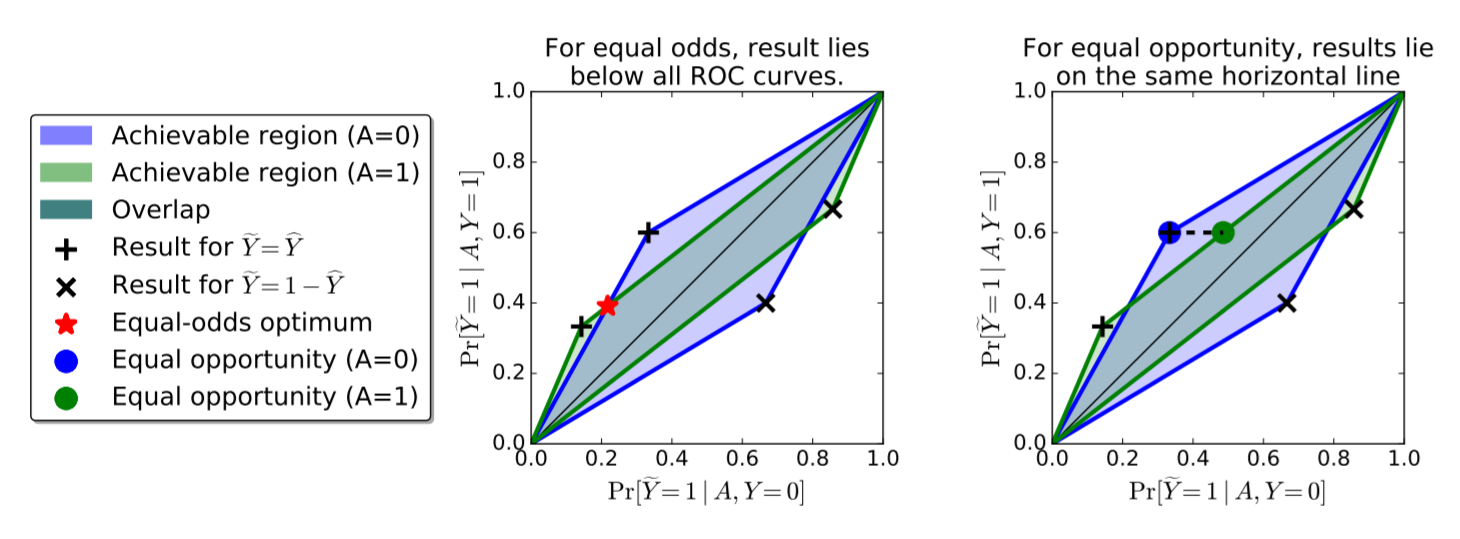
\includegraphics[width=15.0cm]{posexample.png}
	\caption{Búsqueda del clasificador óptimo para los criterios de probabilidades igualadas e igualdad de oportunidad, respectivamente. (\cite{eodd2016})}
    \label{fig:posprocessing}
\end{figure}

\subsection*{Ventajas e inconvenientes}

Los algoritmos de posprocesamiento comparten algunas ventajas con los de preprocesamiento, pudiéndose aplicar de forma independiente al modelo de clasificación sin necesidad de modificar su método de actuación. Además, consigue un rendimiento relativamente bueno en la optimización de la mayoría de definiciones de equidad (a excepción de la  equidad contrafactual).

Sin embargo, se puede argumentar que al actuar sobre el modelo después de haberlo aprendido, este proceso es intrínsecamente subóptimo. Siendo equivalente a aprender a sabiendas un modelo sesgado y luego corregirlo, en lugar de aprender un modelo insesgado desde el principio.

\subsection*{Otros ejemplos en la literatura}

En el artículo presentado por \cite{woodworth2017} se amplía el trabajo de \cite{eodd2016}, demostrando que su método de posprocesamiento podría ser subóptimo en algunos casos. Se ofrece una demostración de que el problema es intratable, y se presenta un método que aproxima el criterio de equidad proporcionando un resultado estadísticamente cercano al óptimo.

\ctparttext{\color{black}\begin{center}
Discusión sobre la inferencia causal, el cálculo de contrafactuales y el teorema de incompatibilidad como fundamentos matemáticos de la equidad contrafactual.
\end{center}}
\part{Fundamentos de la equidad contrafactual} \label{part:fundamentoseqcontra}

\chapter{Inferencia causal} \label{ch:inferenciacau}

En este capítulo formalizaremos algunos conceptos básicos para desarrollar la teoría relativa a la causalidad en el ámbito de la equidad. Además, introduciremos los grafos como herramienta para describir los modelos causales explicados, así como los efectos que tienen estos modelos en las poblaciones donde se aplican.

\section{Modelos causales}

Elegiremos los \textit{modelos causales estructurales} aprovechando que pueden ofrecernos una base sólida para las diferentes nociones causales utilizadas en este trabajo. La forma más sencilla de conceptualizar un modelo causal estructural, es como un programa que genera una distribución a partir de \textit{variables de ruido} independientes mediante una secuencia de instrucciones formales. 

Imaginemos que en lugar de muestras de una distribución, tenemos un programa informático que genera muestras a partir de una semilla aleatoria. El código de este programa, partiría de una semilla aleatoria simple e iría construyendo muestras cada vez más complejas. Esta idea es la misma que utiliza un modelo causal estructural cambiando la sintaxis de programación por lenguaje matemático.

\subsection{Ejemplo: Construcción de un modelo causal} \label{subsec:sobrepeso}

Supongamos una población en la que un individuo hace ejercicio regularmente con una probabilidad de $\frac{1}{2}$. Con una probabilidad de $\frac{1}{3}$, el individuo tiene predisposición a desarrollar sobrepeso en ausencia de ejercicio regular. Del mismo modo, en ausencia de ejercicio, la aparición de una enfermedad cardíaca puede aparecer con una probabilidad de $\frac{1}{3}$. Denotaremos por $X$ el indicador de ejercicio regular, por $Y$ el de exceso de peso, y por $Z$ el indicador de la enfermedad cardíaca. A continuación, construiremos un modelo causal estructural para generar muestras de esta población hipotética (\cite{fairnesslearning2019}).

\clearpage

\begin{algorithm}[h]
\caption{Programa distribución causal 1.}
    Muestras de variables aleatorias independientes de Bernoulli:
    
    $U_1 \sim  Bernoulli\left(\frac{1}{2}\right), \ U_2,U_3 \sim  Bernoulli\left(\frac{1}{3}\right)$\;
    $X:=U_1$\;
    $Y:=$ \textbf{if} $X=1$ \textbf{then} $0$ \textbf{else} $U_2$\;
    $Z:=$ \textbf{if} $X=1$ \textbf{then} $0$ \textbf{else} $U_3$\;
    \label{alg:programa2}
\end{algorithm}

A partir de la descripción anterior, observamos que en nuestra población el ejercicio evita tanto el sobrepeso como las enfermedades cardíacas, pero en ausencia de ejercicio, ambos son independientes. Nuestro programa genera una distribución conjunta sobre las variables aleatorias $(X, Y, Z)$. Podemos calcular las probabilidades bajo esta distribución. Por ejemplo, la probabilidad de sufrir una enfermedad cardíaca bajo la distribución especificada por nuestro modelo es de $\frac{1}{2}\cdot \frac{1}{3}=\frac{1}{6}$. También podemos calcular la probabilidad condicional de padecer enfermedades cardíacas dado el sobrepeso. Dado el suceso $Y = 1$ podemos inferir que el individuo no hace ejercicio $X=0$, por lo que la probabilidad de sufrir una enfermedad cardíaca debido al sobrepeso es $\frac{1}{3}$.

Formalmente, tener un programa que genere una distribución es más potente que el simple acceso al muestreo. Una de las razones es que podemos manipular el programa de la manera que queramos, mientras resulte en un programa funcional. Podríamos, por ejemplo, establecer $Y := 1$, dando lugar a una nueva distribución. El programa resultante tiene el siguiente aspecto:

\begin{algorithm}[h]
\caption{Programa distribución causal 2.}
    Muestras de variables aleatorias independientes de Bernoulli:
    
    $U_1 \sim  Bernoulli\left(\frac{1}{2}\right), \ U_2,U_3 \sim  Bernoulli\left(\frac{1}{3}\right)$\;
    $X:=U_1$\;
    $Y:=1$\;
    $Z:=$ \textbf{if} $X=1$ \textbf{then} $0$ \textbf{else} $U_3$\;
\end{algorithm}

Calculando de nuevo la probabilidad de sufrir una enfermedad cardíaca sobre la nueva distribución, de nuevo obtenemos $\frac{1}{6}$. Este cálculo revela una idea importante, la sustitución $Y := 1$ no corresponde a un condicionamiento de $Y = 1$. Una se trata de una acción y la otra es una observación de la que podemos extraer conclusiones. En este ejemplo, si observamos que un individuo tiene sobrepeso, podemos inferir que tiene un mayor riesgo de enfermedad cardíaca. Sin embargo, esto no significa que la reducción del peso corporal evite las enfermedades cardíacas. En cambio, la intervención $Y := 1$ crea un nuevo modelo en el que todos los individuos de la población tienen sobrepeso con todo lo que ello conlleva.

A continuación, profundizaremos un poco más en este punto considerando otra población hipotética, especificada por el siguiente programa:

\begin{algorithm}[h]
\caption{Programa distribución causal 3.}
    Muestras de variables aleatorias independientes de Bernoulli:
     
    $U_1 \sim  Bernoulli\left(\frac{1}{2}\right), \ U_2,U_3 \sim  Bernoulli\left(\frac{1}{3}\right)$\;
    $Y:=U_2$\;
    $X:=$ \textbf{if} $Y=0$ \textbf{then} $0$ \textbf{else} $U_1$\;
    $Z:=$ \textbf{if} $X=1$ \textbf{then} $0$ \textbf{else} $U_3$\;
    \label{alg:programa3}
\end{algorithm}

En esta población, la única razón por la que los individuos eligen hacer ejercicio con cierta probabilidad es el sobrepeso. Por otro lado, las enfermedades del corazón se desarrollan en ausencia de ejercicio. La sustitución $Y := 1$ en este modelo conduce a un aumento de la probabilidad de hacer ejercicio y por tanto, a una disminución de la probabilidad de sufrir una enfermedad cardíaca. El condicionamiento de $Y = 1$ también tiene el mismo efecto y en ambos casos, la probabilidad de sufrir un problema cardíaco es de  $\frac{1}{6}$.

\subsection{Formalización de los modelos causales estructurales}

Los modelos causales estructurales nos proporcionan un cálculo preciso para razonar sobre el efecto de las acciones hipotéticas. Formalmente, un modelo causal estructural es una secuencia de asignaciones que generan una distribución conjunta a partir de variables de ruido independientes. A continuación ofreceremos la definición de modelo causal estructural presentada por \cite{causality2000}.\\

\begin{definition}[Modelo causal estructural] \label{def:modcausalest}
Un \textit{modelo causal estructural} $M$ se define como una tupla $(U,V,F)$ de conjuntos tales que:
\begin{itemize}
    \item $U$ es un conjunto de variables aleatorias de ruido, las cuales deben ser conjuntamente independientes. Corresponden a factores no causados por ninguna variable del conjunto $V$ de variables observadas.
    \item $F$ es un conjunto de funciones $\{f_1,\dots,f_n\}$, una para cada $V_i\in V$, tal que, $$V_i=f_i(pa_i,U_i), \ \text{para todo} \ i=1,\dots,n.$$
    donde $pa_i \subseteq V \setminus \{V_i\}$ y $U_i \subseteq U$. Estas ecuaciones también son conocidas como \textit{ecuaciones estructurales}.
\end{itemize}
\end{definition}\

El modelo es causal en el sentido de que, dada una distribución de probabilidad $P(U)$ sobre las variables de ruido $U$, podemos derivar la distribución de un subconjunto $W \subseteq V$ tras una intervención en $V \setminus W$. Cuando $M$ denota un modelo causal estructural, escribiremos la probabilidad de un evento $E$ bajo la distribución conjunta vinculada como $P_M(E)$. 

Para familiarizarnos con la notación, supongamos que $M$ denota el modelo causal estructural del Apartado \ref{subsec:sobrepeso}, entonces la probabilidad de sufrir una enfermedad cardíaca en este modelo será $P_M(Z) = \frac{1}{6}$.

\section{Grafos causales}

La notación $pa_i$ utilizada en la Definición \ref{def:modcausalest}, se refiere al subconjunto de variables $pa(V_i)$ que contiene los padres del nodo $V_i$. Esta notación viene motivada por la suposición de que el modelo se factoriza como un grafo dirigido, el cual en este trabajo, restringiremos al caso acíclico (DAG). A este grafo lo llamaremos: el \textit{grafo o diagrama causal} correspondiente al modelo causal estructural especificado.\\

\begin{figure}[h]
\centering
\begin{tikzpicture}[
  node distance=1cm and 1cm,
  mynode/.style={draw,circle,text width=0.5cm,align=center}
]

\node[mynode] (z) {$X$};
\node[mynode,below left=of z] (x) {$Y$};
\node[mynode, below right=of z] (y) {$Z$};

\node[mynode,right=of y] (a) {$Y$};
\node[mynode,above right=of a] (b) {$X$};
\node[mynode,below right=of b] (c) {$Z$};

\path (z) edge[-latex] (x)
(z) edge[-latex] (y);

\path (a) edge[-latex] (b)
(c) edge[latex-] (b);

\end{tikzpicture}
\caption{Grafos causales de los modelos descritos por los Programas \ref{alg:programa2} y \ref{alg:programa3}, respectivamente.}
\end{figure}

Los diagramas causales se utilizan cuando las asignaciones exactas en un modelo causal estructural son secundarias, y lo que es realmente relevante son los caminos presentes y ausentes entre nodos. Los grafos también nos permiten aprovechar el lenguaje de teoría de grafos para discutir nociones causales. En particular, los grafos causales nos ayudan a distinguir la causa y el efecto (de tipo directo o indirecto), en función de si un nodo es ancestro o descendiente de otro.

\subsection{Forks}

\begin{definition} [\textit{Fork}]
Sea $G$ un grafo acíclico dirigido, $U$ el camino entre dos nodos y $A\in U$. Llamaremos \textit{fork} al nodo $A$ si $(A,B)\in E$, para todo $B\in ve(A) \cap U$.
\end{definition}\

\begin{figure}[h]
\centering
\begin{tikzpicture}[
  node distance=1cm and 1cm,
  mynode/.style={draw,circle,text width=0.5cm,align=center}
]

\node[mynode] (z) {A};
\node[mynode,below left=of z] (x) {B};
\node[mynode, below right=of z] (y) {C};

\path (z) edge[-latex] (x)
(z) edge[-latex] (y);

\end{tikzpicture}
\caption{Ejemplo de \textit{fork}.}
\label{fig:fork}
\end{figure}

\clearpage

En la Figura \ref{fig:fork} el nodo $A$ es un ejemplo de \textit{fork} o dicho de otro modo, el nodo $A$ es la causa común de los nodos $B$ y $C$. En el grafo causal resultante de la distribución del Programa $\ref{alg:programa2}$, el nodo $X$ también es un ejemplo de \textit{fork} ($Y \leftarrow X \to Z$). En ese caso la variable indicadora de ejercicio regular $X$ influía, tanto en el aumento de peso $Y$, como en el riesgo de enfermedad $Z$. Sin embargo, como ya discutimos en el Apartado \ref{subsec:sobrepeso}, las variables $Y$ y $Z$ no están correlacionadas positivamente. Llegamos a la conclusión de que el nodo \textit{fork}, tiene un efecto de confusión que conduce a un desacuerdo entre el cálculo de las probabilidades condicionales y las intervenciones. 

\begin{example}
En un conocido estudio médico, un presunto efecto beneficioso de la terapia de sustitución hormonal para reducir las enfermedades cardiovasculares, desapareció tras identificar el estatus socioeconómico como variable de confusión (\cite{ejconfusion2002}). Los ejemplos de confusión suponen una amenaza para la validez de las conclusiones extraídas de los datos en problemas del mundo real.
\end{example}

\subsection{Colliders}

\begin{definition} [\textit{Collider}]
Sea $G$ un grafo acíclico dirigido, $U$ el camino entre dos nodos y $A\in U$. Llamaremos \textit{collider} al nodo a $A$ si $(B,A)\in E$, para todo $B\in ve(A) \cap U$.
\end{definition}

\begin{figure}[h]
\centering
\begin{tikzpicture}[
  node distance=1cm and 1cm,
  mynode/.style={draw,circle,text width=0.5cm,align=center}
]

\node[mynode,right=of y] (a) {B};
\node[mynode,above right=of a] (b) {A};
\node[mynode,below right=of b] (c) {C};

\path (a) edge[-latex] (b)
(b) edge[latex-] (c);

\end{tikzpicture}
\caption{Ejemplo de \textit{collider}.}
\label{fig:collider}
\end{figure}\

En la Figura \ref{fig:collider} el nodo $A$ es un ejemplo de \textit{collider}. Cabe destacar que los \textit{colliders}, no dan lugar a situaciones en las que se pueda dar confusión. De hecho en la figura anterior, la relación entre $B$ y $C$ no es confusa, lo que significa que podemos sustituir las intervenciones por probabilidades condicionales. Sin embargo, condicionar un \textit{collider} podría crear una correlación entre $B$ y $C$, un fenómeno al que denominaremos sesgo de \textit{collider}. 

\begin{example}
En el ámbito sanitario, dos enfermedades independientes pueden correlacionarse negativamente cuando se analizan pacientes hospitalizados. La razón es que cuando cualquiera de las dos enfermedades ($B$ o $C$) es suficiente para el ingreso en el hospital (indicado por la variable $A$), observar que un paciente tiene una enfermedad hace que la otra sea estadísticamente menos probable. A esto es lo que se le conoce como paradoja de Berkson (\cite{berksonparadox2014}).
\end{example}

\subsection{Mediador}

En la definición de \textit{fork}, no tenemos una relación directa entre los nodos $B$ y $C$. Si queremos un efecto total de $B$ sobre $C$ estableceremos esta relación causal a través de $A$. En este caso, $A$ no será un factor confusión y recibirá el nombre de \textit{mediador}.\\

\begin{figure}[h]
\centering
\begin{tikzpicture}[
  node distance=1cm and 1cm,
  mynode/.style={draw,circle,text width=0.5cm,align=center}
]

\node[mynode] (z) {A};
\node[mynode,below left=of z] (x) {B};
\node[mynode, below right=of z] (y) {C};

\path (x) edge[-latex] (z)
(z) edge[-latex] (y);

\end{tikzpicture}
\caption{Ejemplo de mediador.}
\label{fig:mediator}
\end{figure}

En el grafo causal asociado a la distribución generada por el Programa \ref{alg:programa3}, el nodo $X$ es un ejemplo de mediador ($Y \to X \to Z$). La noción de mediador es especialmente relevante para el tema del análisis de la discriminación, ya que establece una relación directa entre las diferentes variables que definen a un individuo. Esta relación causal nos servirá como herramienta para extraer conclusiones sobre las causas de segregación entre grupos.

\section{Intervención y confusión}

Los modelos causales estructurales nos proporcionan una herramienta de formalización del efecto de acciones e intervenciones sobre la población donde se aplican. Como hemos visto previamente, para modelar estos efectos simplemente necesitamos la capacidad de realizar sustituciones.

\subsection{Operadores para realizar actuaciones en el modelo}

A partir de los ejemplos propuestos en el Apartado \ref{subsec:sobrepeso}, hemos observado que fijar una variable por sustitución puede corresponder o no a una probabilidad condicional. Esto refuerza nuestra intuición de que una observación no es una acción. En cambio, una sustitución sí es una acción, ya que al sustituir un valor estamos rompiendo el curso natural de la acción captada por nuestro modelo.\\

\begin{definition}[Intervención]
Dado un modelo causal estructural $M$, se define una \textit{intervención} sobre una variable observada $X$, como la sustitución de la ecuación $X:=f(pa,U)$ por la ecuación $X:=x$ para un valor $x$ constante.
\end{definition}

\clearpage

Denotaremos el modelo resultante por $M' = M[X := x]$, para indicar la modificación que realizamos sobre el modelo original $M$. Bajo esta asignación mantenemos $X$ constante, eliminando la influencia de sus nodos padres, y por tanto de cualquier otra variable del modelo. Por otra parte, los nodos hijos de $X$ recibirán un valor constante $x$ cuando consulten el valor de su padre.\\

\begin{figure}[h]
\centering
\begin{tikzpicture}[
  node distance=1cm and 1cm,
  mynode/.style={draw,circle,text width=0.5cm,align=center}
]

\node[mynode] (z) {$X$};
\node[mynode,above=of z] (u) {$P_2$};
\node[mynode,above left=of z] (v) {$P_1$};
\node[mynode,above right=of z] (w) {$P_3$};
\node[mynode,below=of z] (s) {$H_2$};
\node[mynode,below left=of z] (x) {$H_1$};
\node[mynode, below right=of z] (y) {$H_3$};

\node[mynode,right=of y] (a) {$H_1$};
\node[mynode,above right=of a] (b) {$X$};
\node[mynode,above=of b] (c) {$P_2$};
\node[mynode,above right=of b] (d) {$P_3$};
\node[mynode,above left=of b] (e) {$P_1$};
\node[mynode,below=of b] (f) {$H_2$};
\node[mynode,below right=of b] (g) {$H_3$};

\path (z) edge[-latex] (x)
(z) edge[-latex] (y)
(z) edge[-latex] (s)
(v) edge[-latex] (z)
(u) edge[-latex] (z)
(w) edge[-latex] (z);

\path (b) edge[-latex] (a)
(b) edge[-latex] (f)
(b) edge[-latex] (g);

\end{tikzpicture}
\caption{Grafo causal antes y después de la sustitución.}
\end{figure}

El operador de asignación también se denomina \textit{operador do}, para destacar que corresponde a la realización de una acción o intervención. La notación que usaremos para calcular las probabilidades dado un evento cualquiera $E$ después de aplicar el \textit{operador do}, será $P_{M[X:=x]}(E)$. También podemos utilizar otra notación equivalente, que aproxima el concepto de probabilidad condicional, y que se define como: 
\begin{equation*}
P(E \mid \text{do}(X:=x))=P_{M[X:=x]}(E).
\end{equation*}

\subsection{Confusión entre dos variables}

Las cuestiones importantes en inferencia causal, están vinculadas a cuándo podemos reescribir una \textit{operación do} en términos de probabilidades condicionales. Cuando esto sea posible, podremos estimar el efecto de la operación a partir de las probabilidades condicionales estimadas de los datos. 

Sea una variable $Y$, sobre la que actúa una variable $X$, nos interesará que exista una equivalencia entre el efecto causal de la acción y la probabilidad condicional correspondiente, es decir, que se cumpla la siguiente igualdad: 
\begin{equation*}
P(Y=y \mid \text{do}(X:=x))=P(Y=y \mid X=x).
\end{equation*}

En general, esto no es cierto. Al fin y al cabo, la diferencia entre la observación (probabilidad condicional) y la acción (intervención) es la principal motivación de la inferencia causal.\\

\begin{definition}[Confusión]
Sean $Y$ una variable aleatoria sobre la que actúa otra variable $X$, diremos que son \textit{confusas} si, y solo si, $$P(Y=y \mid \text{do}(X:=x)) \neq P(Y=y \mid X=x).$$
\end{definition}\

Cuando tenemos dos variables aleatorias confusas, podemos estimar el efecto de una intervención en términos de probabilidades condicionales a partir de la denominada \textit{fórmula de ajuste}.\\

\begin{proposition} \label{prop:forajuste}
Sean $X,Y$ dos variables confusas, podemos aproximar el efecto causal de una intervención dada a partir de probabilidades condicionales como: $$P(Y=y \mid \text{do}(X:=x))=\sum_{z}P(Y=y \mid X=x,PA=z)P(PA=z),$$
donde $PA$ indica el conjunto $pa(X)$.
\end{proposition}\

Dependiendo de la estructura del grafo, podremos eliminar o no la confusión entre dos variables utilizando la fórmula de ajuste sobre un nodo u otro. Si el grafo tiene una estructura de \textit{fork} (por ejemplo, $B \leftarrow A \to C$), eliminaremos la confusión entre los nodos $B$ y $C$, condicionando $A$. En cualquier otro caso (mediador o \textit{collider}), ajustar una variable tendría consecuencias opuestas a las que buscamos.

\subsection*{Criterio de \textit{backdoor}}

El tratamiento de la confusión a partir de la fórmula de ajuste, puede ser una tarea complicada cuando la cantidad de nodos en el grafo aumente considerablemente. Para detectar las variables sobre las que deberemos condicionar, aparece el \textit{criterio de backdoor} (\cite{causality2000}). Este método parte de la idea de seleccionar un conjunto de variables, que bloqueen todos los \textit{caminos de backdoor} entre los dos nodos sobre los que queremos eliminar la confusión.\\

\begin{definition}[Camino de \textit{backdoor}]
Un \textit{camino de backdoor} entre dos nodos $A$ y $B$, es cualquier camino que empiece con una arista de la forma ''$\leftarrow$'' hacia $A$.
\end{definition}\

\begin{definition}[Conjunto de \textit{backdoor}]
Un \textit{conjunto de backdoor}, es una secuencia de variables o nodos contenida en un camino de \textit{backdoor}.
\end{definition}\

Para aplicar el criterio de \textit{backdoor}, primero seleccionaremos un conjunto de \textit{backdoor} del grafo. Si el conjunto está formado por una secuencia de nodos relacionados únicamente por aristas de tipo ''$\to$'', podremos eliminar la confusión entre las variables, aplicando la fórmula de ajuste sobre un nodo central de la cadena. Por otro lado, si el camino contiene un \textit{collider} o un descendiente de este, la confusión es inevitable, ya que bloqueando el camino podríamos impedir que la información fluyera a través de los nodos.

\begin{example}
Sea un grafo causal dado por la secuencia $A \leftarrow C \to D \to E \to B$, nuestro objetivo será eliminar la confusión entre las variables $A$ y $B$. Es evidente que la cadena $A \leftarrow C \to D \to E \to B$ es un camino de \textit{backdoor}. A continuación, seleccionamos un conjunto de \textit{backdoor} entre ambos nodos, por ejemplo $C \to D \to E$. En vista de la forma de la secuencia anterior, podemos eliminar la confusión entre $A$ y $B$ aplicando la fórmula de ajuste sobre el nodo $D$.
\end{example}

\subsection*{Confusión no observada}

La fórmula de ajuste presentada en la Proposición \ref{prop:forajuste}, podría sugerir que siempre podemos eliminar el sesgo de confusión condicionando a los nodos padres. Sin embargo, esto no se cumple cuando aparecen \textit{factores de confusión no observados}. En la práctica, a menudo hay variables que son difíciles de medir o que no fueron resgistradas. Podemos incluir estos nodos no observados en un grafo, indicando su influencia con líneas discontinuas.\\

\begin{figure}[h]
\centering
\begin{tikzpicture}[
  node distance=1cm and 1cm,
  mynode/.style={draw,circle,text width=0.5cm,align=center}
]

\node[mynode] (z) {C};
\node[mynode,below left=of z] (x) {A};
\node[mynode, below right=of z] (y) {B};

\node[mynode,right=of y] (a) {A};
\node[mynode,above right=of a] (b) {C};
\node[mynode,right=of b] (d) {D};
\node[mynode,below right=of d] (c) {B};

\path (z) edge[dashed, -latex] (x)
(z) edge[dashed, -latex] (y);

\path (b) edge[dashed, -latex] (d)
(a) edge[dashed, latex-] (b)
(d) edge[-latex] (c);

\end{tikzpicture}
\caption{Ejemplos de confusión no observada.}
\label{fig:unobserved}
\end{figure}

La Figura \ref{fig:unobserved} muestra dos casos de confusión no observada. En el primer ejemplo, el efecto causal de $A$ sobre $B$ no es identificable. En el segundo caso, podemos eliminar la confusión entre $A$ y $B$ a partir del criterio de \textit{backdoor}. Sea $C \to D \to B$ un conjunto de \textit{backdoor}, podemos eliminar la confusión entre las variables $A$ y $B$ ajustando la fórmula sobre la variable $D$ aunque $C$ no se observe.

Cabe destacar que podemos combatir la confusión no observada aumentando el número de variables consideradas, pero esto aumentaría progresivamente la complejidad de nuestro modelo causal. En la práctica, es habitual controlar el mayor número posible de variables con el objetivo de eliminar el sesgo de confusión. Sin embargo, como hemos visto, el control de mediadores y \textit{colliders} podría ser problemático en la resolución de nuestro problema.

\chapter{Teorema de imposibilidad de la equidad} \label{ch:teoremaimposibilidad}

En este capítulo se propondrá una demostración alternativa del teorema de imposibilidad de equidad. Este enunciado surge como una formalización de la \textit{incompatibilidad} entre los criterios de paridad demográfica, probabilidades igualadas y tasa de paridad predictiva.

\section{Caracterización del teorema}

La mayoría de los criterios de equidad definidos en el Capítulo \ref{ch:formalmedeq}, se construyen a partir de restricciones no triviales de la distribución de probabilidad conjunta. Por ello, es lógico pensar que la imposición de varios de ellos de forma simultánea, restringirían el espacio de búsqueda hasta el punto de que solo obtendríamos soluciones degeneradas.

El teorema de la imposibilidad, cuya primera aproximación fue ofrecida por \cite{fairth2016}, establece que no se puede satisfacer más de una medida de equidad al mismo tiempo para un clasificador bien entrenado y un atributo sensible que sea capaz de introducir un sesgo en el modelo. En nuestro caso, presentaremos una versión del teorema para tres de los criterios de equidad de grupo estudiados: paridad demográfica, tasa de paridad predictiva y probabilidades igualadas. Los enunciados de los lemas demostrados, a lo largo de este capítulo, han sido definidos en base al trabajo de \cite{fairnesslearning2019}.


\subsection{Paridad demográfica vs. Tasa de paridad predictiva}

Comenzamos con un lema que muestra cómo, en general, la paridad demográfica y la paridad predictiva se excluyen mutuamente. La única suposición necesaria es que el atributo sensible $A$ y la variable $Y$ no sean independientes, es decir, dependen una de la otra. Esto es una forma diferente de decir, que un grupo tiene mayor tasa de resultados positivos que otro, lo que es cierto en la mayoría de casos.

\clearpage

\begin{lemma} 
Supongamos que $A$ e $Y$ son variables dependientes. Entonces, la paridad demográfica ($\hat{Y} \perp A$) y la tasa de paridad predictiva ($Y \perp A \mid \hat{Y}$), no pueden verificarse simultáneamente.
\label{lem:demopred}
\end{lemma}

\begin{proof}
El enunciado del lema es análogo a la siguiente expresión,
\begin{equation*}
Y \not \perp A \quad \Longrightarrow \quad \neg(\hat{Y} \perp A \ \wedge \ Y \perp A \mid \hat{Y}).
\end{equation*}

Procederemos por contrarrecíproco, lo que equivale a demostrar que,
\begin{equation*}
\hat{Y} \perp A \ \wedge \ Y \perp A \mid \hat{Y} \quad \Longrightarrow \quad Y \perp A.
\end{equation*}

Si se da la independencia entre las variables $A$ e $\hat{Y}$, entonces se cumple,
\begin{equation}\label{eq:lema1eq1}
P(A=a,\hat{Y}=\hat{y})=P(A=a)P(\hat{Y}=\hat{y}).
\end{equation}

Por otro lado, sabemos que la independencia condicional dada por $Y \perp A \mid \hat{Y}$ satisface que,
\begin{equation}\label{eq:lema1eq2}
P(Y=y, A=a \mid \hat{Y}=\hat{y})=P(Y=y\mid \hat{Y}=\hat{y})P(A=a\mid \hat{Y}=\hat{y}).
\end{equation}

Finalmente, aplicando las hipótesis del enunciado y usando el teorema de probabilidad total (T.P.T) sobre $P(Y=y,A=a)$, llegamos a la siguiente expresión:
\begin{equation*}
\begin{split}
P(Y=y,A=a)&\overset{\text{T.P.T}}{=}\sum_{\hat{y}} P(\hat{Y}=\hat{y})P(Y=y,A=a \mid \hat{Y}=\hat{y})\\
&\overset{(\ref{eq:lema1eq2})}{=} \sum_{\hat{y}} P(\hat{Y}=\hat{y})P(Y=y\mid \hat{Y}=\hat{y})P(A=a \mid \hat{Y}=\hat{y})\\
&= \sum_{\hat{y}} P(\hat{Y}=\hat{y})P(Y=y\mid \hat{Y}=\hat{y})\ddfrac{P(A=a,\hat{Y}=\hat{y})}{P(\hat{Y}=\hat{y})}\\
&\overset{(\ref{eq:lema1eq1})}{=} \sum_{\hat{y}} P(\hat{Y}=\hat{y})P(Y=y\mid \hat{Y}=\hat{y})\ddfrac{P(A=a)P(\hat{Y}=\hat{y})}{P(\hat{Y}=\hat{y})}\\
&=\sum_{\hat{y}} P(\hat{Y}=\hat{y})P(Y=y\mid \hat{Y}=\hat{y})P(A=a)\\
&=P(A=a)\sum_{\hat{y}} P(\hat{Y}=\hat{y})P(Y=y\mid \hat{Y}=\hat{y})\\
&\overset{\text{T.P.T}}{=}P(A=a)P(Y=y).
\end{split}
\end{equation*}

La última igualdad nos da que las variables $A$ e $Y$ son independientes y por tanto tenemos que $Y\perp A$.
\end{proof}

\subsection{Paridad demográfica vs. Probabilidades igualadas}

Un resultado análogo de exclusión mutua, es válido para la paridad demográfica y el criterio de probabilidades igualadas. El enunciado, en este caso, es un poco más rebuscado y requiere la suposición adicional de que la variable $Y$ sea binaria. También necesitamos que la variable $\hat{Y}$ dependa de $Y$. Esta suposición es una relajación bastante suave, ya que cualquier función de clasificación útil tiene correlación con la variable $Y$.\\

\begin{lemma} 
Supongamos que $Y$ es una variable binaria, $A$ e $Y$ son dependientes y además, $Y$  también depende de $\hat{Y}$. Entonces, la paridad demográfica ($\hat{Y} \perp A$) y el criterio de las probabilidades igualadas ($\hat{Y} \perp A \mid Y$), no pueden verificarse simultáneamente.
\label{lem:demoigu}
\end{lemma}

\begin{proof}
El enunciado del lema es equivalente a la siguiente expresión,
\begin{equation*}
Y \not \perp A \ \wedge \ Y \not \perp \hat{Y} \quad \Longrightarrow \quad \neg(\hat{Y} \perp A \ \wedge \ \hat{Y} \perp A \mid Y).
\end{equation*}

Por el contrarrecíproco, deberemos demostrar que,
\begin{equation*}
\hat{Y} \perp A \ \wedge \ \hat{Y} \perp A \mid Y
 \quad \Longrightarrow \quad Y  \perp A \ \vee \ Y  \perp \hat{Y}.
\end{equation*}

Si se da la independencia entre las variables $A$ e $\hat{Y}$, entonces se cumple,
\begin{equation}\label{eq:lema2eq1}
P(\hat{Y}=\hat{y},A=a)=P(\hat{Y}=\hat{y})P(A=a).
\end{equation}

Sabemos que la independencia condicional dada por $\hat{Y} \perp A \mid Y$ satisface que,
\begin{equation}\label{eq:lema2eq2}
P(\hat{Y}=\hat{y} \mid A=a, Y=y)=P(\hat{Y}=\hat{y} \mid Y=y).
\end{equation}

Aplicando el teorema de la probabilidad total (T.P.T) y la hipótesis de independencia condicional sobre $P(\hat{Y}=\hat{y} \mid A=a)$, obtenemos la siguiente expresión:
\begin{equation}\label{eq:lema2eq3}
\begin{split}
P(\hat{Y}=\hat{y} \mid A=a) &\overset{\text{T.P.T}}{=} \sum_{y} P(Y=y \mid A=a) P(\hat{Y}=\hat{y} \mid A=a, Y=y)\\
&\overset{(\ref{eq:lema2eq2})}{=} \sum_{y} P(Y=y \mid A=a)P(\hat{Y}=\hat{y} \mid Y=y).
\end{split}
\end{equation}

Usando la hipótesis de independencia entre las variables $A$ e $\hat{Y}$,
\begin{equation}\label{eq:lema2eq4}
\begin{split}
P(\hat{Y}=\hat{y} \mid A=a) &= \ddfrac{P(\hat{Y}=\hat{y},A=a)}{P(A=a)}\\ &\overset{(\ref{eq:lema2eq1})}{=} \ddfrac{P(\hat{Y}=\hat{y})P(A=a)}{P(A=a)}\\
&= P(\hat{Y}=\hat{y}).
\end{split}
\end{equation}

Combinando las Ecuaciones (\ref{eq:lema2eq3}) y (\ref{eq:lema2eq4}), llegamos a la siguiente expresión:
\begin{equation}\label{eq:lema2eq5}
P(\hat{Y}=\hat{y}) = \sum_{y} P(Y=y \mid A=a)P(\hat{Y}=\hat{y} \mid Y=y).
\end{equation}

Por otro lado, aplicando el teorema de la probabilidad total sobre $P(\hat{Y}=\hat{y})$, tenemos que,
\begin{equation}\label{eq:lema2eq6}
P(\hat{Y}=\hat{y}) = \sum_{y} P(Y=y) P(\hat{Y}=\hat{y} \mid Y=y).
\end{equation}

Combinando las Ecuaciones (\ref{eq:lema2eq5}) y (\ref{eq:lema2eq6}), conseguimos la expresión dada por:
\begin{equation}\label{eq:lema2eq7}
\sum_{y} P(Y=y \mid A=a)P(\hat{Y}=\hat{y} \mid Y=y) = \sum_{y} P(Y=y) P(\hat{Y}=\hat{y} \mid Y=y).
\end{equation}

A continuación, y para que sea más cómodo de manipular la expresión anterior definiremos la siguiente notación:
\begin{equation*}
\begin{split}
    p&=P(Y=0),\\
    p_a&=P(Y=0 \mid A=a),\\
    \hat{y}_{y}&=P(\hat{Y}=\hat{y} \mid Y=y).
\end{split}
\end{equation*}

Por hipótesis del Lema, $Y$ es una variable binaria (supongamos que puede tomar los valores $0$ o $1$) y por tanto, podemos reescribir la Ecuación (\ref{eq:lema2eq7}) como:
\begin{equation*}
p\hat{y}_0+(1-p)\hat{y}_1=p_a\hat{y}_0+(1-p_a)\hat{y}_1.
\end{equation*}

Simplificando en la ecuación anterior, tenemos que,
\begin{equation*}
p(\hat{y}_0-\hat{y}_1)=p_a(\hat{y}_0-\hat{y}_1),
\end{equation*}
lo cual es equivalente a,
\begin{equation}\label{eq:lema2eq8}
(p-p_a)(\hat{y}_0-\hat{y}_1)=0.
\end{equation}

La igualdad de la Ecuación (\ref{eq:lema2eq8}), se satisface si se da alguno de los siguientes casos:

\begin{itemize}
    \item $p=p_a$, que es equivalente a $P(Y=0)=P(Y=0 \mid A=a)$, y por tanto tenemos,
    \begin{equation*}
    \begin{split}
    P(Y=1)&=1-P(Y=0)\\
    &=1-P(Y=0 \mid A=a)\\
    &=P(Y=1 \mid A=a),
    \end{split}
    \end{equation*}
    donde la expresión anterior equivale a que $Y\perp A$.\\
    
    \item $\hat{y}_0=\hat{y}_1$, que equivale a $P(\hat{Y}=\hat{y}\mid Y=0)=P(\hat{Y}=\hat{y}\mid Y=1)$, y por tanto tenemos que $\hat{Y}\perp Y$.
\end{itemize}


\end{proof}


\subsection{Probabilidades igualadas vs. Tasa de paridad predictiva}

Por último, pasamos a la relación entre la tasa de paridad predictiva y el criterio de probabilidades igualadas. Ambas exigen una relación de independencia condicional no trivial entre las tres variables $A$, $\hat{Y}$ e $Y$. Imponer ambas simultáneamente, conduce a un espacio de soluciones degenerado, como afirma el corolario siguiente.\\

\begin{corollary}
Supongamos que todos los sucesos en la distribución conjunta $(A,\hat{Y},Y)$ tienen probabilidad positiva, y además $A$ depende de $Y$. Entonces, el criterio de probabilidades igualadas ($\hat{Y}\perp A \mid Y$) y la tasa de paridad predictiva ($Y\perp A \mid \hat{Y}$), no pueden verificarse simultáneamente.
\label{cor:probpositiva}
\end{corollary}

\begin{proof}
El enunciado del corolario es análogo a la siguiente expresión,
\begin{equation*}
Y \not \perp A \quad \Longrightarrow \quad \neg(\hat{Y} \perp A \mid Y \ \wedge \ Y \perp A \mid \hat{Y}).
\end{equation*}

Por el contrarrecíproco, tenemos que probar que,
\begin{equation*}
\hat{Y} \perp A \mid Y \ \wedge \ Y \perp A \mid \hat{Y} \quad \Longrightarrow \quad Y \perp A.
\end{equation*}

Por la propiedad simétrica de la independencia condicional, tenemos que,
\begin{equation*}
\begin{split}
\hat{Y} \perp A \mid Y &= A \perp \hat{Y} \mid Y,\\
Y \perp A \mid \hat{Y} &= A \perp Y \mid \hat{Y}.\\
\end{split}
\end{equation*}


La hipótesis dada por $A \perp \hat{Y} \mid Y$ satisface que,
\begin{equation}\label{eq:lema3eq1}
P(A=a \mid \hat{Y}=\hat{y}, Y=y)=P(A=a \mid Y=y).
\end{equation}

Por otro lado, sabemos que $A \perp Y \mid \hat{Y}$ cumple que,
\begin{equation}\label{eq:lema3eq2}
P(A=a \mid Y=y, \hat{Y}=\hat{y})=P(A=a\mid \hat{Y}=\hat{y}).
\end{equation}

Para que tengan sentido las Ecuaciones (\ref{eq:lema3eq1}) y (\ref{eq:lema3eq2}), es necesaria la hipótesis de que $P(\hat{Y}=\hat{y},Y=y)>0$ que a su vez, es consecuencia directa de que la distribución conjunta $(A,\hat{Y},Y)$ tenga probabilidad positiva.

Por la propiedad de unión débil de la independencia condicional, tenemos que las Ecuaciones (\ref{eq:lema3eq1}) y (\ref{eq:lema3eq2}) son equivalentes, y por tanto:
\begin{equation}\label{eq:lema3eq3}
P(A=a\mid Y=y)=P(A=a\mid \hat{Y}=\hat{y}).
\end{equation}

Usando la definición de probabilidad condicionada sobre $P(A=a\mid Y=y)$, tenemos que, 
\begin{equation}\label{eq:lema3eq5}
P(A=a\mid Y=y)=\ddfrac{P(A=a,Y=y)}{P(Y=y)},
\end{equation}
queremos demostrar que $Y\perp A$, es decir, $P(A=a,Y=y)=P(A=a)P(Y=y)$, que aplicado a la Ecuación (\ref{eq:lema3eq5}), equivale a probar:
\begin{equation*}
P(A=a\mid Y=y)=P(A=a).
\end{equation*}

Usando el teorema de la probabilidad total (T.P.T) sobre $P(A)$, conseguimos la siguiente expresión:
\begin{equation*}
\begin{split}
P(A=a)&\overset{\text{T.P.T}}{=}\sum_{\hat{y}}P(\hat{Y}=\hat{y})P(A=a \mid \hat{Y}=\hat{y})\\
&\overset{(\ref{eq:lema3eq3})}{=}\sum_{\hat{y}}P(\hat{Y}=\hat{y})P(A=a \mid Y=y)\\
&=P(A=a \mid Y=y)\sum_{\hat{y}}P(\hat{Y}=\hat{y})\\
&=P(A=a \mid Y=y).
\end{split}
\end{equation*}
\end{proof}

Para un objetivo binario, la hipótesis de no degeneración del Corolario  \ref{cor:probpositiva} establece que en todos los grupos, para todos los valores de predicción, tenemos casos positivos y negativos. En caso de que el clasificador sea binario, podemos debilitar la suposición exigiendo que el clasificador haga al menos una predicción falsa positiva. Lo atractivo de la afirmación resultante es, que su prueba se basa esencialmente en una relación bastante popular entre la tasa de verdaderos positivos (\textit{Recall}) y el valor predictivo positivo (\textit{Precision}).\\

\begin{lemma}
Supongamos que $\hat{Y}$ es una variable binaria que toma valores de un clasificador con una tasa de falsos positivos no nula, y además $A$ dependiente de $Y$. Entonces, el criterio de probabilidades igualadas ($\hat{Y}\perp A \mid Y$) y la tasa de paridad predictiva ($Y\perp A \mid \hat{Y}$), no pueden verificarse simultáneamente.
\label{lem:preigual}
\end{lemma}

\begin{proof}
Dado que $Y \not \perp A$, existirán dos grupos, a los que llamaremos $p_0$ y $p_1$ cumpliendo que $p_0\neq p_1$, donde $p_a=P(Y=1 \mid A=a)$.

Supondremos que se satisface el criterio de las probabilidades igualadas. Por hipótesis, el clasificador tendrá la misma tasa para todos los grupos de falsos y verdaderos positivos (FPR,TPR $> 0$). Procederemos a demostrar que la tasa de paridad predictiva no se satisface en estas condiciones.

En el caso binario, la tasa de paridad predictiva implica que todos los grupos tienen el mismo de PPV (ver Apartado \ref{subsec:suficiencia}). El valor predictivo positivo en el grupo $a$, denotado PPV$_a$ satisface
\begin{equation*}
    \text{PPV}_a = \ddfrac{\text{TPR}p_a}{\text{TPR}p_a+\text{FPR}(1-p_a)}.
\end{equation*}

De la expresión anterior vemos que: PPV$_0$ = PPV$_1$ si, y solo si, TPR $= 0$ o FPR $= 0$. Descartaremos esto último por hipótesis. Por tanto, se debe cumplir que TPR $= 0$.  Sin embargo, podemos deducir que NPV$_0 \neq$ NPV$_1$ a partir de la siguiente expresión,
\begin{equation*}
    \text{NPV}_a = \ddfrac{(1-\text{FPR})(1-p_a)}{(1-\text{TPR})p_a+(1-\text{FPR})(1-p_a)}.
\end{equation*}

Por tanto, la tasa de paridad predictiva no se satisface.
\end{proof}

\subsection{Enunciado y demostración}

Una vez demostrados los resultados previos, estamos preparados para enunciar y demostrar la versión del teorema de imposibilidad para la equidad de grupo.\\

\begin{theorem}[Teorema de imposibilidad de la equidad] \label{th:teoimpos}
Consideremos un problema de clasificación binaria con una tasa de falsos positivos no nula, donde se cumple la siguiente relación de dependencia entre las variables: $Y \not \perp A$ e $\hat{Y} \not \perp Y$. Si existe una asignación de riesgo, entonces ésta no puede satisfacer los criterios de paridad demográfica, probabilidades igualadas y paridad predictiva simultáneamente dos a dos.
\end{theorem}

\begin{proof}
Bajo las hipótesis del teorema, aplicamos los Lemas \ref{lem:demopred}, \ref{lem:demoigu} y \ref{lem:preigual}.
\end{proof}

\section{Perspectiva causal} \label{sec:saravaku}

Podemos consultar una versión diferente de la demostración del Teorema \ref{th:teoimpos}, desde la perspectiva de la inferencia causal, en el artículo propuesto por \cite{impossibilityth2021}. Además, el artículo presenta una propuesta teórica de corrección de los datos de entrenamiento, con el objetivo de mitigar el sesgo presente en el mismo y ajustarlo a las nociones de equidad actuales que pudiesen cambiar con el tiempo.\vspace{7mm}

\begin{figure}[h]
\centering
\begin{tikzpicture}[
  node distance=1cm and 1cm,
  mynode/.style={draw,circle, minimum width=1.2cm},
]
\node[mynode] (z) {$Y$};
\node[mynode,right=of z] (x) {$\hat{Y}$};
\node[mynode,below=of z] (y) {$A$};
\node[mynode,below=of x] (w) {$C$};
\node[mynode,right=of w, fill={rgb:black,1;white,2}] (e) {$U_C$};
\draw[-latex] (z) -- (x);
\draw[-latex] (y) -- (z);
\draw[-latex] (w) -- (x);
\draw[-latex] (e) -- (w);
\draw[-latex] (y) -- (w);
\end{tikzpicture}
\caption{Diagrama causal con la variable de corrección.}
\label{fig:varcorrect}
\end{figure}

\clearpage

El diagrama causal para el proceso de generación de datos puede representarse, como podemos observar en la Figura \ref{fig:varcorrect}, introduciendo una variable de corrección $C$ que determinará si la información de la etiqueta verdadera $Y$ debe propagarse a la predicción $\hat{Y}$ o no. 

La variable de corrección se define como una función dependiente del atributo sensible ($C \not\perp A$), pero que no permite el paso de la información de $A$ a través de ella. Por otro lado, el flujo de información de $Y$ a $\hat{Y}$ no tiene que estar necesariamente bloqueado para el grupo favorecido, esto es deseable si queremos evitar el sesgo sobre el grupo marginado.\\

\begin{figure}[h]
\centering
\begin{tikzpicture}[
  node distance=1cm and 1cm,
  mynode/.style={draw,circle, minimum width=1.4cm},
]
\node[mynode, fill={rgb:green,1;white,3}] (z) {$Y$};
\node[mynode,right=of z, fill={rgb:red,1;white,3}] (x) {$\hat{Y}$};
\node[mynode,below=of z] (y) {$A$};
\node[mynode,below=of x, font=\small] (w) {$C=0$};
\node[mynode,right=of w, fill={rgb:black,1;white,2}] (e) {$U_C$};
\node[mynode,right=of e] (f) {$A$};
\node[mynode,right=of f, font=\small] (g) {$C=1$};
\node[mynode,right=of g, fill={rgb:black,1;white,2}] (h) {$U_C$};
\node[mynode,above=of g, fill={rgb:green,1;white,3}] (i) {$\hat{Y}$};
\node[mynode,above=of f, fill={rgb:green,1;white,3}] (j) {$Y$};
\draw[-latex] (z) -- (x);
\draw[-latex] (y) -- (z);
\draw[-latex] (w) -- (x);
\draw[-latex] (e) -- (w);
\draw[-latex] (y) -- (w);
\draw[latex-] (j) -- (f);
\draw[latex-] (g) -- (f);
\draw[latex-] (g) -- (h);
\draw[-latex] (g) -- (i);
\draw[latex-] (g) -- (h);
\draw[-latex] (j) -- (i);
\draw (0.8,-0.5) -- (1.5,0.5);
\end{tikzpicture}
\caption{Efecto de la variable de corrección.}
\label{fig:effectcorrec}
\end{figure}\

\begin{proposition} 
Sea $g$ un clasificador arbitrario y $U_C$ una variable de ruido para la variable de corrección $C$. Redefinimos la ecuación estructural de $\hat{Y}$ como:
\begin{equation*}
\begin{split}
    f_C &= A \oplus U_C \\
    \hat{Y} &= \left \{
\begin{array}{l l}
g(y), & \mbox{si } C = 1, \\
g(a), & \mbox{si } C =0.
\end{array}
\right.
\end{split}
\end{equation*}
\label{prop:correccion}
\end{proposition}\

La Proposición \ref{prop:correccion} propone la utilización de una corrección del sesgo, eligiendo el grado de desviación de la dependencia de los datos de $Y$. De esta forma, la probabilidad con la que $U_C$ toma el valor 0 o 1, puede ser interpretada como un hiperparámetro ajustable con el objetivo de reflejar cómo de injustos son los datos, y cuánta desviación respecto de los datos históricos se desea alcanzar en el clasificador desarrollado.

Dada esta nueva aproximación, las nociones de paridad demográfica y el criterio de probabilidades igualadas, podrían ser satisfechas conjuntamente ajustando el hiperparámetro $U_C$. Obteniendo las siguientes ecuaciones de equidad modificadas:
\begin{equation*}
    \begin{split}
        \hat{Y} &\perp A \mid (C=0)\\
        \hat{Y} &\perp A \mid Y,C.
    \end{split}
\end{equation*}

\chapter{Medidas causales} \label{ch:medidascausal}

En este capítulo realizaremos un estudio del modelo contrafactual, y cómo sirve de base para diferentes medidas causales, en particular para la equidad contrafactual que discutiremos más detalladamente. 

\section{Contrafactuales}

Una vez definidos los modelos causales estructurales, podemos formular preguntas más delicadas que el mero efecto de una acción. En concreto, preguntas contrafactuales como: ¿Habría evitado el atasco si hubiese tomado otra ruta diferente? o ¿Me habrían concedido el préstamo si mi raza o edad fuesen distintas? Podemos dar respuesta a estas preguntas, a partir de un modelo causal estructural. Sin embargo, el procedimiento para extraer la respuesta del modelo, necesita del cálculo de \textit{contrafactuales}.

\subsection{Ejemplo: Modelo de decisión contrafactual}

Supongamos un problema de decisión entre dos modelos de caja negra para resolver un problema. Denotaremos por $X$ a la variable indicadora de cada algoritmo. Si el problema es irresoluble ($U=1$), ninguno de los algoritmos podrá encontrar una solución. Si el problema es resoluble ($U=0$), un algoritmo obtendrá mejores resultados que el otro. El rendimiento es independientemente de cualquiera de los dos modelos con una probabilidad de $\frac{1}{2}$. Definiremos dos variables aleatorias $U_0, U_1$, que nos informarán del rendimiento para los algoritmos $X=0$ y $X=1$, respectivamente. El modelo seleccionado entre los dos existentes, será elegido al azar por una variable $U_X$ con probabilidad $\frac{1}{2}$. Supondremos también una variable $Y \in \{0,1\}$, que nos dirá si el algoritmo ha encontrado una solución óptima ($Y=0$) o no ($Y=1$). A continuación especificaremos el modelo discutido con el siguiente programa:

\clearpage

\begin{algorithm}[h]
\caption{Programa distribución contrafactual.}
    Muestras de variables aleatorias independientes de Bernoulli: 
    
    $U,U_0,U_1,U_X \sim  Bernoulli\left(\frac{1}{2}\right)$\;
    $X:=U_X$\;
    $Y:=X \cdot \max\{U,U_1\}+(1-X)\cdot \max\{U,U_0\}$ \;
    \label{alg:programa 4}
\end{algorithm}

El grafo asociado al modelo anterior viene dado por:

\begin{figure}[h]
\centering
\begin{tikzpicture}[
  node distance=1cm and 1cm,
  mynode/.style={draw,circle,text width=0.5cm,align=center}
]

\node[mynode] (z) {X};
\node[mynode,right=of z] (x) {Y};

\path (x) edge[latex-] (z);

\end{tikzpicture}
\caption{Grafo causal asociado al ejemplo.}
\end{figure}

Supongamos que elegimos el algoritmo $X = 1$ y observamos que no consigue una solución $Y = 1$. A continuación, nos hacemos la siguiente pregunta: ¿Habría sido mejor elegir el otro algoritmo? Para responder a ello, calcularemos la probabilidad $P_{M[X:=0]}(Y = 0)$. Dada la sustitución $X := 0$ en nuestro modelo, para que el algoritmo encontrase una solución óptima necesitamos que $\max\{U, U_0\} = 0$. Esto sólo ocurre cuando $U=0$ (con probabilidad $\frac{1}{2}$) y $U_0=0$ (también con probabilidad $\frac{1}{2}$). Concluimos que $P_{M[X:=0]}(Y = 0)=\frac{1}{2}\cdot \frac{1}{2}=\frac{1}{4}$.

Aunque pudiera parecerlo, esta no es la respuesta correcta a nuestra pregunta. La razón es, que hicimos los cálculos sin considerar la decisión previa $\{X = 1, Y = 1\}$. A partir de esta observación, ciertas configuraciones de las variables de ruido $(U, U_0, U_1)$ ya no son factibles. En concreto, si $U$ y $U_1$ hubieran sido ambos cero, habríamos encontrado una solución correcta con el algoritmo $X = 1$, pero esto contradice a nuestra observación $Y=1$. De hecho, la configuración $\{X = 1, Y = 1\}$, sólo permite los valores de la Tabla \ref{tab:contrafactualU} para $U$ y $U_1$.

\begin{table}[h]
\centering
\resizebox{2.0cm}{!} {
\begin{tabular}{cc}
\hline
$U$ & $U_1$ \\ \hline
$0$ & $1$   \\
$1$ & $0$   \\
$1$ & $1$   \\ \hline
\end{tabular}
}
\caption{Posibles valores de las variables de ruido dada la evidencia observada.}
\label{tab:contrafactualU}
\end{table}

Cada uno de estos tres casos, es igualmente probable, lo que en particular significa que el evento $U = 1$ tiene una probabilidad de $\frac{2}{3}$. Sin considerar la observación, recordemos que $U = 1$ tenía una probabilidad de $\frac{1}{2}$. Por lo que la evidencia observada $\{X = 1, Y = 1\}$, ha sesgado la distribución de la variable de ruido $U$ hacia el valor $1$. Utilizaremos la letra $U'$ para referirnos a esta versión sesgada de $U$.

Podemos volver a considerar el efecto de la acción $X := 0$ sobre el resultado $Y$, trabajando ahora con la nueva variable $U'$. Para $Y = 0$, necesitamos que $\max \{U', U_0\} = 0$. Esto significa que $U' = 0$, un suceso que ahora tiene probabilidad $\frac{1}{3}$, y $U_0 = 0$ (con probabilidad $\frac{1}{2}$, igual que antes). Por lo tanto, obtenemos que una vez actualizado el modelo, $P_{M'[X:=0]}(Y = 0)=\frac{1}{3}\cdot \frac{1}{2}=\frac{1}{6}$.

Si comparamos el nuevo valor con el resultado anterior, tenemos que la incorporación de las observaciones disponibles en nuestro cálculo, disminuyó la probabilidad de que encontrásemos la solución óptima con el otro algoritmo,
\begin{equation*}
    P_{M'[X:=0]}(Y = 0)=\frac{1}{6} < \frac{1}{4}=P_{M[X:=0]}(Y = 0).
\end{equation*}

La razón de ello es que el evento observado, sesga la distribución de las variables de ruido haciendo que fuese incluso más probable que en general, el problema no tuviese solución. Llamaremos al resultado que acabamos de calcular: el valor contrafactual al elegir el algoritmo alternativo, dado que el algoritmo seleccionado no encontró una solución óptima.


\subsection{Formalización del cálculo contrafactual}

Sea $M=(U,V,F)$ un modelo causal estructural, la especificación de $F$ es un supuesto fuerte que permite el cálculo de valores contrafactuales. Calcularemos el valor de $Y$, si $Z$ hubiera tomado el valor $z$, como la solución de $Y$ para un $U := u$ dado, en el que las ecuaciones de $Z$ se sustituyen por $Z := z$. Denotaremos la expresión anterior por $Y_{Z\leftarrow z}(U)$ (\cite{causality2000}).

La \textit{inferencia contrafactual}, especificada por un modelo causal $M$ dada la evidencia $E$, equivale al cálculo de $P(Y_{Z\leftarrow z}(U) \mid E = e)$, donde $E, Z, Y \subseteq V$. Existen tres pasos esenciales en el cálculo de contrafactuales: incorporar las observaciones sesgando las variables de ruido mediante una operación de condicionamiento, realizar una \textit{operación do} en el modelo causal después de sustituir las variables de ruido sesgadas y finalmente, calcular la distribución para una variable objetivo. Estos tres pasos se denominan \textit{abducción, acción} y \textit{predicción}, y se definen de la siguiente manera:\\

\begin{definition}[Cálculo del contrafactual] \label{def:pasoscontra}
Dado un modelo causal estructural $M$, un evento observado $E$, una intervención $Z := z$ y una variable objetivo $Y$, definimos el \textit{contrafactual} $Y_{Z \leftarrow z}(E)$ mediante los siguientes pasos:

\begin{itemize}
    \item \textit{Abducción}: Condicionar la distribución conjunta de $U = (U_1,\dots,U_n)$ al suceso $E$. Esto da lugar a una distribución sesgada $U'=P(U \mid E=e)$.
    \item \textit{Acción}: Utilizar el \textit{operador do}, para realizar la intervención $Z := z$ en el modelo causal estructural $M$, obteniendo el modelo $M' = M[Z := z]$.
    \item \textit{Predicción}: Calcular el objetivo contrafactual $Y_{Z \leftarrow z}(E)$ usando $U'$ como semilla aleatoria en $M'$.
\end{itemize}
\end{definition}


\section{Equidad contrafactual}

Todos los criterios de equidad definidos en el Capítulo \ref{ch:formalmedeq}, tienen limitaciones en su aplicación a problemas reales. Mientras que la equidad por desconocimiento es un criterio insuficiente debido a la gran cantidad de características correlacionadas con los atributos sensibles, la equidad individual tiene el problema de ser directamente dependiende de una distancia fiable entre individuos. Por otro lado, los criterios de equidad de grupo, son observacionales y no pueden utilizarse para encontrar la causa de la disparidad entre grupos. 

Como solución a estos problemas, aparecen las \textit{medidas causales} donde, en este trabajo, profundizaremos en la \textit{equidad contrafactual} (\cite{worlds2017}) que puede ser considerada como una subclase de las mismas. Este concepto considera que, para un individuo, una decisión es justa si coincide en el mundo real y en un mundo ''contrafactual'' en el que el individuo perteneciese a un grupo demográfico diferente. Esta suposición construye un método para comprobar el tratamiento dispar, que surge al sustituir únicamente el atributo sensible y además, proporciona una explicación del impacto del sesgo a través de un grafo causal.\\

\begin{definition}[Equidad contrafactual]
Dado $A\in \mathcal{A}$ un atributo sensible multivaluado, $g\colon \mathcal{X} \to \mathcal{Y}$ un clasificador arbitrario, $X \in \mathcal{X}\setminus \mathcal{A}$ una variable observada cualquiera y $(U,V,F)$ un modelo causal donde $V \equiv A \cup X$. Se dice que $g$ satisface la \textit{equidad contrafactual} si, y solo si, $$P(\hat{Y}_{A\shortleftarrow a}(U)=y \mid X=x, A=a)=P(\hat{Y}_{A\shortleftarrow a'}(U)=y \mid X=x, A=a),$$
para todo $y$ y $a'\neq a$. 
\end{definition}\

\begin{figure}[h]
\centering   
\begin{tikzcd}[m]
  & |[opacity=0]|\mm{A}{raza} & \\
   \mm{S}{estudios} \arrow[drr] & &\arrow[ll] \mm{J}{trabajo}\\
  |[w]| \mm{U}{motivación} \arrow[u] \arrow[rr]& & \mm{Y}{graduado}\\
\end{tikzcd}\qquad
\begin{tikzcd}[m]
  & \mm{A}{raza}\arrow[dr] & \\
   \mm{S}{estudios} \arrow[drr] & &\arrow[ll] \mm{J}{trabajo}\\
  |[w]| \mm{U}{motivación} \arrow[u] \arrow[rr]& & \mm{Y}{graduado}\\
\end{tikzcd}\qquad
\begin{tikzcd}[m]
  & \mm{A}{raza}\arrow[dl]\arrow[dr] & \\
   \mm{S}{estudios} \arrow[drr] & &\arrow[ll] \mm{J}{trabajo}\arrow[d]\\
  |[w]| \mm{U}{motivación} \arrow[u] \arrow[rr]& & \mm{Y}{graduado}\\
\end{tikzcd}
\caption{Ejemplo de grafo causal en un problema real.}
\label{fig:caugraph}
\end{figure}

La Figura \ref{fig:caugraph} muestra varios ejemplos sobre un caso relacionado con la admisión a la universidad (\cite{worlds2017}). Si sustituimos el atributo sensible (raza) por su valor contrafactual, todas las características correlacionadas con él también se verían influidas (estudios y trabajo), propagándose hacia abajo en el grafo causal a través de las ecuaciones estructurales. Cualquier atributo que no descienda del atributo sensible permanecerá igual.

\subsection{Implicaciones de la definición de equidad}

En este apartado, presentaremos algunas implicaciones de la definición de equidad contrafactual, y algunos resultados que proporcionan un método directo para satisfacer esta noción de justicia dado un modelo (\cite{counterfactual2018}).\\

\begin{lemma} \label{lem:nodescent}
Sea $G$ el grafo causal del modelo dado por $(U,V,F)$, $A\in \mathcal{A}$ un atributo sensible multivaluado y $g\colon \mathcal{X} \to \mathcal{Y}$ un clasificador arbitrario. Entonces $g$ satisface la equidad contrafactual, si es una función que no depende de los nodos descendientes de $A$.
\end{lemma}

\begin{proof}
Sea $W$ una variable no descendiente de $A$ en $G$. Entonces $W_{A\leftarrow a}(U)$ y $W_{A\leftarrow a'}(U)$ tienen la misma distribución para los tres pasos de la Definición \ref{def:pasoscontra}. Por lo tanto, la distribución de cualquier función $g$ de los nodos no descendientes de $A$, es invariante con respecto a los valores contrafactuales de $A$.
\end{proof}

\begin{comment}
\subsection*{Solución a problemas de otras nociones de equidad}

La equidad contrafactual también proporciona una respuesta a algunos problemas sobre la incompatibilidad de los criterios de equidad. Supongamos el caso en el que nos gustaría que nuestro clasificador cumpliese el criterio de igualdad de oportunidades y la tasa de paridad predictiva simultáneamente. Se demostró, en el Capítulo \ref{ch:teoremaimposibilidad}, que esto es imposible. La equidad contrafactual nos aporta una solución en este escenario sugiriendo, que tanto la igualdad de oportunidades como la paridad predictiva, pueden ser insuficientes si $A$ e $Y$ están asociados: suponiendo que las variables no son confusas, esto es el resultado de que $A$ sea una causa de $Y$. 

Como estamos en el ámbito de la equidad contrafactual, no deberíamos utilizar $Y$ como base para nuestras decisiones, en lugar de ello, deberíamos buscar una función de variables que no sean causadas por $A$ pero que puedan predecir $Y$, a este conjunto de funciones lo denotaremos por $Y_{\perp A}$. Definiremos entonces $\hat{Y}$ como una estimación de la $Y_{\perp A}$ más cercana a $Y$, usando como guía alguna función de riesgo. Esto hace que la incompatibilidad entre el criterio de igualdad de oportunidades y paridad predictiva sea irrelevante, ya que $A$ e $Y_{\perp A}$ serán independientes por como las hemos construido dadas las suposiciones del modelo.

\subsection*{Tratamiento de los prejuicios históricos y la paradoja de la equidad existente}

La diferencia explícita entre $\hat{Y}$ e $Y$ nos permite abordar los sesgos históricos. Por ejemplo, supongamos que $Y$ es un indicador de si un cliente no devuelve un préstamo, mientras que $\hat{Y}$ es la decisión real de conceder el préstamo. Consideremos el grafo causal que se muestra en la Figura \ref{fig:grafotratam} con la inclusión explícita del conjunto $U$ de variables de ruido independientes. En principio, $Y$ es la medida objetivamente ideal para la toma de decisiones, ya que indica si el cliente dejó de pagar o no el préstamo. Si $A$ es un atributo protegido, entonces el clasificador definido por $\hat{Y} = Y = f_Y (A, U)$ no satisface la equidad contrafactual, siendo la flecha $A \to Y$ el resultado de un mundo que perjudica a los individuos de una manera que está fuera de su control. Por tanto, el principio de equidad contrafactual nos prohíbe utilizar $Y$.\\

\begin{figure}[h]
\centering
\begin{tikzpicture}[
  node distance=1cm and 1cm,
  mynode/.style={draw,circle,text width=0.5cm,align=center}
]

\node[mynode, fill={rgb:black,1;white,2}] (z) {A};
\node[mynode,right=of z, fill={rgb:black,1;white,2}] (x) {Y};
\node[mynode,left=of z] (y) {$U_A$};
\node[mynode,right=of x] (w) {$U_Y$};

\path (x) edge[latex-] (z);
\path (y) edge[-latex] (z);
\path (x) edge[latex-] (w);

\end{tikzpicture}
\caption{Grafo causal donde $A$ es un atributo sensible e $Y$ un resultado de interés.}
\label{fig:grafotratam}
\end{figure}

Por el contrario, cualquier función de variables no descendientes de $A$ puede utilizarse como base para la toma de decisiones justas. Esto significa que cualquier variable $\hat{Y}$ definida por $\hat{Y} = g(U)$ satisface la equidad contrafactual para cualquier función $g(\cdot)$. Por lo tanto, dado un modelo causal, el funcional definido por $g(\cdot)$ que minimiza algún error de predicción para $Y$ cumplirá la equidad contrafactual, como se propone en la Sección \ref{sec:algoritmo}. En esencia, estamos aprendiendo una proyección de $Y$ en el espacio de las decisiones justas, eliminando de paso los posibles sesgos históricos existentes.
\end{comment}

\subsection*{Defectos y limitaciones}

El concepto de equidad contrafactual, teóricamente hablando, puede parecer una buena idea para eliminar todos los defectos del resto de criterios estudiados. En la práctica, la dependencia de conceptos como la inferencia causal o el estudio de contrafactuales lo hacen una de las nociones de equidad más complejas de implementar. 

Otro problema surge cuando queremos acordar cómo debería ser el grafo causal, o decidir qué características vamos a utilizar incluso disponiendo de dicho grafo. Esto se debe a que podríamos perder precisión si rechazamos variables de estudio que pudiesen ser problemáticas a la hora de realizar el estudio causal.

\ctparttext{\color{black}\begin{center}
Elaboración de un ejemplo práctico sobre la equidad contrafactual y su discusión frente a otras nociones de equidad estudiadas.
\end{center}}
\part{Análisis experimental}  \label{part:analisis_exp}


\chapter{Descripción y diseño} \label{ch:descdise}

En este capítulo se describirá un problema real de justicia en el ámbito de la educación, y se propondrán varios diseños de modelos causales que puedan ser tratados por un algoritmo de equidad contrafactual, con el objetivo de eliminar el tratamiento dispar en el problema.

\section{Algoritmo de aprendizaje justo}

\label{sec:algoritmo}

El algoritmo propuesto por \cite{counterfactual2018} parte de la necesidad de relacionar $\hat{Y}$ con $Y$. Para ello restringiremos $\hat{Y}$ para que funcione como una función parametrizada de los nodos no descendientes de $A$ apoyándonos en el Lema \ref{lem:nodescent}. 

Calculemos la predicción $\hat{Y}$ a partir de un clasificador parametrizado por $\btheta$ al que denominaremos como $g_{\btheta}(U,X_{\not \succ A})$, donde $X_{\not \succ A} \subseteq X$ denota el conjunto de no descendientes de $A$. Dada una función de pérdida $l(\cdot,\cdot)$ (\textit{squared} o \textit{logistic loss}) y un conjunto de datos $\mathcal{D}=\{(A^{(i)},X^{(i)},Y^{(i)}) \ : \ i=1,\dots,n\}$, definimos $$L(\btheta)=\displaystyle \frac{1}{n} \sum_{i=1}^n \mathbb{E}[l(y^{(i')},g_{\btheta}(U^{(i')},x_{\not \succ A}^{(i')}))\mid x^{(i)},a^{(i)}],$$ como la pérdida empírica al minimizar sobre $\btheta$. Cada esperanza se calcula respecto a la variable $U^{(i)} \sim P_{\mathcal{M}}(U \mid x^{(i)},a^{(i)})$, donde $P_{\mathcal{M}}(U \mid x,a)$ es la distribución condicional de las variables de ruido dada por el modelo causal $\mathcal{M}$. En tiempo de predicción, crearemos una nueva variable $\tilde{Y}=\mathbb{E}[\hat{Y}(U^\ast,x_{\not \succ A}^\ast)\mid x^\ast, a^\ast]$ para un nuevo elemento del conjunto de datos $(a^\ast,x^\ast)$. 

Para aproximar la esperanza, utilizaremos el \textit{método de Monte Carlo basado en cadenas de Markov} o MCMC (\cite{mcmc2003}). Los métodos MCMC son una clase de algoritmos de simulación para el muestreo y estimación de distribuciones de probabilidad a posteriori. Al construir un cadena de Markov usando una distribución deseada como distribución de equilibrio de la cadena, se puede hacer un muestreo de la distribución, registrando los diferentes estados del grafo. Cuántas más iteraciones realicemos con el método de Monte Carlo, la distribución de la cadena se acercará más a la distribución real deseada.

\begin{algorithm}[h]
\caption{FairLearning($\mathcal{D},\mathcal{M}$)}
\label{alg:fairlearn}
    \KwIn{$\mathcal{D}$, conjunto de datos y $\mathcal{M}$, modelo causal.}
    \KwOut{parámetros aprendidos $\htheta$.}
    \For{$ i\in \mathcal{D}$}{
    muestrear $m$ ejemplos MCMC $U_1^{(i)},\dots,U_m^{(i)} \sim P_{\mathcal{M}}(U \mid x^{(i)},a^{(i)})$.
    }
    Creamos $\mathcal{D}'$ donde cada punto $(a^{(i)},x^{(i)},y^{(i)})$ en $\mathcal{D}$ es sustituido por los 
    
    correspondientes $m$ puntos $\{(a^{(i)},x^{(i)},y^{(i)},u_j^{(i)})\}$\;
    $\htheta \leftarrow \text{argmin}_{\btheta} \sum_{i'\in \mathcal{D}'} l(y^{(i')},g_{\btheta}(U^{(i')},x_{\not \succ A}^{(i')}))$\;
   \textbf{devolver} $g_{\htheta}$\;
\end{algorithm}

\section{Diseño del modelo causal de entrada}

\label{sec:modeloentrada}

El modelo $\mathcal{M}$ debe proporcionarse al Algoritmo \ref{alg:fairlearn}; recordemos que los modelos causales requieren de fuertes suposiciones cuando se hacen afirmaciones contrafactuales (\cite{fairnesslearning2019}). Existen infinitas ecuaciones estructurales compatibles con la misma distribución observable; por lo que, teóricamente estos modelos deberían ser propensos a modificaciones si, por ejemplo se incorporan nuevos datos anteriormente no observados que contradijesen el modelo actual.

En nuestro trabajo, no será necesario especificar un modelo totalmente determinista y relajaremos las ecuaciones estructurales a partir de la definición de distribución condicional. En particular, el concepto de equidad contrafactual es válido bajo los siguientes tres niveles, que vienen especificados en el trabajo de \cite{counterfactual2018} como:

\begin{itemize}
    \item \textbf{Nivel 1}: predecir $\hat{Y}$ usando sólo las variables observables no descendientes de $A$. Esta consideración no requiere de ninguna suposición causal, pero en la mayoría de los problemas la mayor parte de las variables observables serán descendientes de atributos protegidos, y por tanto tendremos menos información manejable.
    \item \textbf{Nivel 2}: suponer variables de ruido que actúan como causas no deterministas de las variables observables, basadas en el conocimiento explícito del dominio y en algoritmos de aprendizaje. La información sobre $X$ pasará a $\hat{Y}$ a través de $P(U \mid x, a)$.
    \item \textbf{Nivel 3:} construir un modelo totalmente determinista con variables de ruido. Por ejemplo, la distribución $P(V_i \mid pa_i)$ puede tratarse como un modelo de error aditivo, $V_i =f_i(pa_i)+\epsilon_i$ (\cite{noise2014}). El término de error $\epsilon_i$ sirve como una entrada a $\hat{Y}$ calculada a partir de las variables observadas. Esto maximizará la información extraída por el clasificador.
\end{itemize}

\section{Aplicación en un problema real}

Ilustraremos la aplicación de justicia contrafactual sobre un problema del mundo real que requiere equidad. El objetivo de este experimento es cuantificar el comportamiento del Algoritmo \ref{alg:fairlearn} con tamaños de muestra finitos sobre una suposición real compatible con un modelo sintético.

\subsection{Descripción del problema} \label{subsec:desproblem}

El Consejo de Admisión de las Facultades de Derecho realizó una encuesta en 163 facultades de Derecho de Estados Unidos (\cite{lsac1998}). Contiene información sobre 21.790 estudiantes de Derecho, tales como las puntuaciones de su examen de acceso (LSAT), su media del expediente (GPA) antes de entrar en la facultad, y su nota media del primer año (FYA) en la carrera de Derecho.

A partir de estos datos, una escuela podría querer predecir si un solicitante tendrá un FYA alto. También podría ser interesante asegurarse de que estas predicciones no están sesgadas por la raza y el sexo del individuo. Sin embargo, es bastante probable que los resultados del LSAT, GPA y FYA estén sesgados por factores sociales. Nuestro trabajo consistirá en aplicar las herramientas aprendidas para equidad contrafactual en diversos escenarios y comparar su actuación con otras nociones de equidad estudiadas.

\subsection{Escenarios de predicción} \label{subsec:escenariospred}

Utilizaremos el mismo escenario de experimentación que el propuesto en \cite{counterfactual2018}. Dividiremos el conjunto de datos en un 80-20 (entrenamiento-test) para evaluar los modelos, preservando el equilibrio de las etiquetas. Para predecir los resultados utilizaremos un predictor basado en regresión lineal, y mediremos la exactitud alcanzada por cada modelo a con la métrica RMSE y el coeficiente de determinación.  

Según hemos descrito en la Sección \ref{sec:modeloentrada}, existen tres aproximaciones a partir de las cuales podemos construir un predictor de FYA que satisfaga la equidad contrafactual: 

\begin{itemize}
    \item \textbf{Nivel 1}: usaremos cualquier característica que no sea descendiente de la raza y el sexo para la predicción. Como suponemos que el LSAT, el GPA y el FYA están sesgados por la raza y el sexo, no podremos utilizar ninguna de las características observadas para construir un clasificador justo contrafactual.
    
    \item \textbf{Nivel 2} (Fair $K$): supondremos que una variable de ruido: los conocimientos del estudiante ($K$), afecta a las puntuaciones de GPA, LSAT y FYA. El gráfico causal correspondiente a este modelo se muestra en la Figura \ref{fig:practicausales}. Emplearemos las siguientes distribuciones:
    \begin{equation*}
    \begin{split}
        \text{GPA} &\sim \mathcal{N}(b_G+K \nm{w}^K_G+[A_R,A_S] \nm{w}^A_G, \sigma_G),\\
        \text{LSAT} &\sim Poisson(\text{exp}(b_L+K \nm{w}^K_L +[A_R,A_S] \nm{w}^A_L)),\\ 
        \text{FYA}&\sim \mathcal{N}(K \nm{w}^K_F+[A_R,A_S] \nm{w}^A_F, 1),\\
        \text{K}&\sim \mathcal{N}(0,1).
    \end{split}
    \end{equation*}
    Realizamos la inferencia sobre este modelo utilizando un conjunto de entrenamiento observado para estimar la distribución posterior de \textit{K}.
    
    \item \textbf{Nivel 3} (Fair $Add$): modelaremos las puntuaciones de GPA, LSAT y FYA como variables continuas con términos de error aditivos independientes de la raza y el sexo. Estimamos los términos de error $\epsilon_G$, $\epsilon_L$ ajustando primero dos modelos que utilizan la raza y el sexo para predecir individualmente el GPA y LSAT. A continuación, calculamos los residuos de cada modelo (aplicando por ejemplo, $\epsilon_G =\text{GPA}-\hat{Y}_{\text{GPA}}(A_R, A_S)$). Finalmente, utilizaremos las estimaciones residuales de $\epsilon_G$, $\epsilon_L$ para predecir FYA. Este modelo se muestra en la Figura \ref{fig:practicausales}. En este caso las distribuciones vienen dadas por:
    \begin{equation*}
    \begin{split}
        \text{GPA} &= b_G+[A_R,A_S] \nm{w}^A_G +\epsilon_G, \ \ \epsilon_G \sim P(\epsilon_G)\\
        \text{LSAT} &= b_L+[A_R,A_S] \nm{w}^A_L +\epsilon_L, \quad \epsilon_L \sim P(\epsilon_L),\\
        \text{FYA}&= b_F+[A_R,A_S] \nm{w}^A_F +\epsilon_F, \quad \epsilon_F \sim P(\epsilon_F).
    \end{split}
    \end{equation*}
\end{itemize}\

\begin{figure}[h]
	\centering
	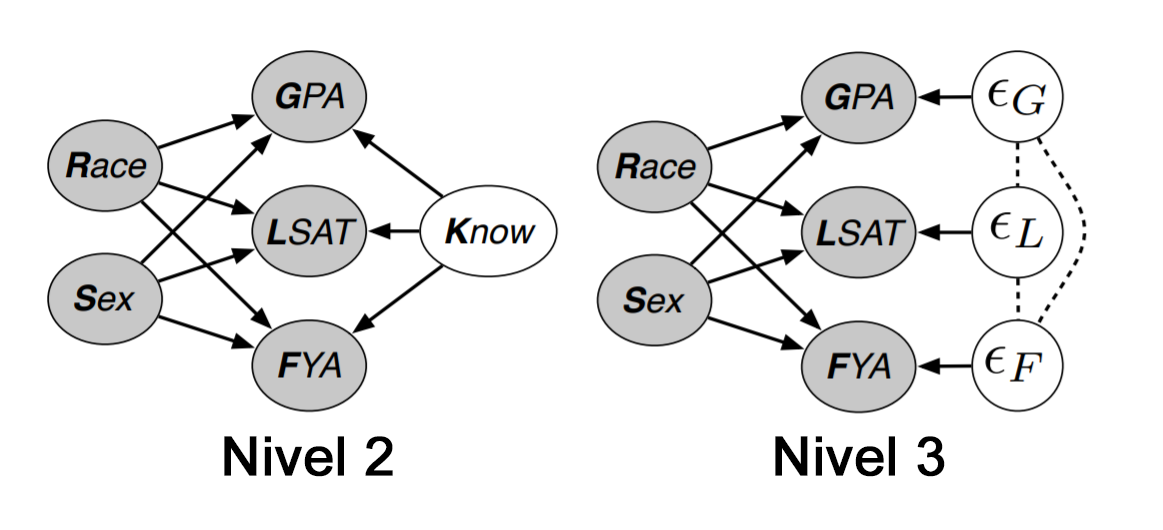
\includegraphics[width=10.8cm]{causales_pract.png}
	\caption{Grafos causales de los escenarios para los niveles 2 y 3, respectivamente.}
    \label{fig:practicausales}
\end{figure}

Compararemos el escenario propuesto por la equidad contrafactual con dos líneas de base injustas: 

\begin{itemize}
    \item \textbf{Modelo completo}: utilizará todas las características disponibles para el individuo, incluidos los atributos sensibles.
    \item \textbf{Modelo por desconocimiento}: aplicaremos la noción de equidad por desconocimiento discutida en la Sección \ref{sec:eqdesconocimiento}.
\end{itemize} 

\chapter{Implementación y resultados} \label{ch:implementaresult}

En este capítulo explicaremos los procedimientos empleados en la implementación de los diseños y algoritmos definidos en el capítulo anterior. Además realizaremos un estudio de la equidad del problema haciendo uso del software Aequitas.

\section{Obtención y tratamiento de los datos}

El conjunto de datos ha sido extraído del repositorio Ethik, que contiene diferentes \textit{datasets} relacionados con el estudio de equidad en aprendizaje automático, y que está disponible en \href{https://github.com/XAI-ANITI/ethik/tree/master/ethik/data}{este enlace}\footnote{https://github.com/XAI-ANITI/ethik/tree/master/ethik/data}.

Es recomendable que antes de aplicar cualquier modelo o algoritmo sobre un conjunto de datos, se realice un tratamiento de los mismos (\texttt{preprocess\_data}). En nuestro caso, haciendo uso de la biblioteca \href{https://pandas.pydata.org/docs/}{Pandas}, hemos realizado las siguientes modificaciones sobre el conjunto de datos original:

\begin{itemize}
    \item Categorizar cada valor del atributo raza, obteniendo una columna para que cada tipo de raza tome el valor 1 o 0 para cada individuo, señalando la pertenencia o no del mismo a la raza indicada por la columna específica (\texttt{get\_dummies}).
    \item Sustituir el atributo sexo por dos columnas ('Male'-'Female'), que indiquen con 1 o 0 la característica del individuo concreto.
    \item Discretizar el valor de 'LSAT' (convertir cada valor a tipo entero).
    \item A partir del análisis del Apartado \ref{ap:facultadderecho}: agrupar los individuos de raza mexicana y puertorriqueña en la raza hispánica, y los de raza amerindia en otras.
\end{itemize}\

\begin{table}[h]
\centering
\resizebox{16.4cm}{!} {
\begin{tabular}{|c|c|c|c|c|c|c|c|c|c|c|c|c|}
\hline
\multicolumn{1}{|l|}{\textbf{UGPA}} & \multicolumn{1}{l|}{\textbf{LSAT}} & \multicolumn{1}{l|}{\textbf{ZFYA}} & \multicolumn{1}{l|}{\textbf{Female}} & \multicolumn{1}{l|}{\textbf{Male}} & \multicolumn{1}{l|}{\textbf{Asian}} & \multicolumn{1}{l|}{\textbf{Black}} & \multicolumn{1}{l|}{\textbf{Hispanic}} & \multicolumn{1}{l|}{\textbf{Other}} & \multicolumn{1}{l|}{\textbf{White}} & \multicolumn{1}{l|}{\textbf{region\_first}} & \multicolumn{1}{l|}{\textbf{sander\_index}} & \multicolumn{1}{l|}{\textbf{first\_pf}} \\ \hline
3.1                                 & 42                                 & 0.36                               & 1                                    & 0                                  & 0                                   & 0                                   & 0                                      & 0                                   & 1                                   & NE                                          & 0.82023                                     & 1                                       \\ \hline
3.3                                 & 39                                 & -0.99                              & 0                                    & 1                                  & 0                                   & 0                                   & 0                                      & 0                                   & 1                                   & NE                                          & 0.80178                                     & 0                                       \\ \hline
2.9                                 & 44                                 & -0.77                              & 0                                    & 1                                  & 1                                   & 0                                   & 0                                      & 0                                   & 0                                   & GL                                          & 0.61369                                     & 1                                       \\ \hline
\end{tabular}
}
\caption{Conjunto \textit{law\_data} tras el preprocesamiento de los datos.}
\label{tab:conjuntosintratar}
\end{table}

\clearpage

Definiremos un array con las categorías de los atributos protegidos, conteniendo los siguientes valores: [''Female'', ''Male'', ''Asian'', ''Black'', ''Hispanic'', ''Other'', ''White'']. Estos serán los valores considerados como sensibles en la definición del problema.

Una vez realizado el tratamiento de los datos, y teniendo el conjunto de datos como se presenta en la Tabla \ref{tab:conjuntosintratar}, almacenaremos los datos útiles en un diccionario (definido a partir de la función \texttt{create\_pystan\_dic}) que nos servirá como estructura de datos contenedora del grafo causal del experimento. Esta elección la realizamos, ya que el método StanModel, que construye el modelo causal, trabaja con diccionarios en Python.

Almacenaremos en el diccionario los siguientes valores:

\begin{itemize}
    \item \textbf{N} - Número total de ejemplos para ese diccionario.
    \item \textbf{C} - Número de categorías diferentes de atributos sensibles.
    \item \textbf{A} - Array con el contenido de cada una de las filas de los atributos protegidos.
    \item \textbf{GPA} - Array con los valores de UGPA.
    \item \textbf{LSAT} - Array con los valores de LSAT.
    \item \textbf{FYA} - Array con los valores de ZFYA.
\end{itemize}

Realizaremos, haciendo uso del método \texttt{train\_test\_split}, una partición del 80-20 para los conjuntos de entrenamiento y test. Crearemos un diccionario para los datos de entrenamiento y otro para los de test (el cuál no contendrá los valores de FYA).

\section{Implementación de los modelos}

El lenguaje de programación seleccionado para la implementación del proyecto ha sido \href{https://docs.python.org/es/3.8/}{Python} en su versión 3.8.5. La elección de Python se debe a que es un lenguaje muy popular en el ámbito de la ciencia de datos, con una gran cantidad de bibliotecas útiles para la visualización de datos y altamente compatible con otros lenguajes de programación que nos pueden ser útiles, tanto para el tratamiento de datos, como para la construcción de modelos causales.

En este apartado, se presentará el diseño de la implementación realizada en Python de forma esquematizada, para más información del funcionamiento de cada modelo, consultar el Capítulo \ref{ch:descdise}. Si por el contrario, quiere consultarse el manual de ejecución del experimento, ir a la Sección \ref{sec:manual}.

\subsection{Modelos injustos}

Como no podemos implementar el nivel 1 presentado en el Apartado \ref{subsec:escenariospred}, ya que el LSAT, GPA y FYA están sesgados por la raza y el sexo. En su lugar (y con el fin de comparar el rendimiento con los modelos de nivel 2 y 3) construiremos los siguientes dos modelos de base injusta.

Para construir los conjuntos con los que entrenaremos en cada modelo, haremos uso de la función \texttt{hstack} de la biblioteca NumPy. Añadiremos según el modelo, los valores específicos de las columnas para los diccionarios pertinentes. Nuestro objetivo será predecir la nota media del primer año para cada individuo (FYA). Utilizaremos un regresor lineal (\texttt{LinearRegression} de la biblioteca Scikit-learn) para predecir el valor de FYA para cada individuo sobre el conjunto de datos de prueba. El regresor, habrá sido previamente entrenado con \texttt{linear\_regresor.fit(x\_train, y\_labels)} usando los datos del conjunto de entrenamiento. Para predecir los valores haremos uso del método \texttt{linear\_regresor.predict(test)}.

\subsection*{Modelo completo}

Funciones creadas para la implementación del \textit{modelo completo}:

\begin{itemize}
    \item \texttt{mod\_full(dic\_train, dic\_test)} :\\ 
    Utilizaremos los datos de entrenamiento (\texttt{dic\_train}) relativos a los atributos protegidos (\texttt{dic\_train['A']}) y los valores de GPA (\texttt{dic\_train['GPA']}) y LSAT (\texttt{dic\_train['LSAT']}). Construiremos el modelo completo, y usaremos el regresor lineal para entrenarlo. Una vez hecho esto, podremos calcular las predicciones sobre el conjunto de datos de prueba (\texttt{dic\_test}).
\end{itemize}

\subsection*{Modelo por desconocimento}

Funciones creadas para la construcción del \textit{modelo por desconocimiento}:

\begin{itemize}
    \item \texttt{mod\_unaware(dic\_train, dic\_test)} :\\
    Usaremos los valores de LSAT (\texttt{dic\_train['LSAT']}) y GPA (\texttt{dic\_train['GPA']}) del conjunto de entrenamiento (\texttt{dic\_train}) para entrenar el modelo. Finalmente, comprobaremos su actuación sobre el conjunto de datos de prueba (\texttt{dic\_test}). En este caso, no utilizamos los atributos protegidos en el entrenamiento.
\end{itemize}

\subsection{Modelos justos}

En este apartado, definiremos las funciones utilizadas para implementar los escenarios de predicción para los niveles 2 y 3 del Apartado \ref{subsec:escenariospred}.

\subsection*{Modelo de variable latente (Fair $K$)}

Para la creación del \textit{modelo de variable latente}, definiremos las siguientes funciones:

\begin{itemize}
    \item \texttt{MCMC(dic\_post, path\_model, path\_stan)} :\\
    Obtenemos las muestras para un modelo Stan (definido en \texttt{path\_stan}) con los datos contenidos en \texttt{dic\_post}. Construiremos el modelo usando la función \texttt{StanModel} de la biblioteca PyStan, lo entrenaremos haciendo uso del método \texttt{sampling} y finalmente extraeremos las muestras con \texttt{extract}. Usaremos 2000 iteraciones y 1 cadena de Markov para replicar el ejemplo de \cite{counterfactual2018}. Para evitar ejecutar el modelo cada vez, guardaremos los modelos entrenados (en \texttt{path\_model}) usando las funciones \texttt{load} y \texttt{dump} del módulo \texttt{pickle}.\\
    \item \texttt{get\_mean\_params(samples, dic\_test)} :\\
    Creamos un diccionario con la media de los parámetros obtenidos en el entrenamiento previo del modelo, almacenados en \texttt{samples}. Mantendremos la estructura del diccionario \texttt{dic\_test} para los parámetros que no varíen, como son $[N, C, A, GPA, LSAT]$, y haremos la media para el resto de parámetros que no dependan de FYA, a saber $[\textbf{w}^K_G, \textbf{w}^A_G, \textbf{w}^K_L, \textbf{w}^A_L, \sigma_G, b_G, b_L]$.\\
    \item \texttt{fair\_learning(dic\_train, dic\_test)} :\\
    Utilizamos el método \texttt{MCMC} sobre el modelo \texttt{law\_school\_train.stan} para obtener las muestras para cada punto del conjunto de datos \texttt{dic\_train}. Guardamos la media de la variable $K$ para \texttt{dic\_train}. Usamos la distribución de $K$ aprendida y hacemos las medias del resto de variables para \texttt{dic\_test}. Volvemos a inferir sobre el modelo, esta vez usando \texttt{law\_school\_only\_k.stan} (sin información sobre FYA) para \texttt{dic\_test}. Finalmente, calculamos la media de la variable $K$ para el conjunto de prueba y la devolveremos junto con la calculada para el conjunto de entrenamiento.\\
    \item \texttt{mod\_fair\_k(dic\_train)} :\\
    Usaremos los arrays con las medias de la variable $K$ inferida en el método anterior, para el conjunto de entrenamiento (\texttt{train\_k}) y el conjunto de prueba (\texttt{test\_k}). Entrenaremos el modelo haciendo uso de la información contenida en \texttt{train\_k} y \texttt{dic\_train['FYA']}. Finalmente usaremos el regresor lineal para calcular las predicciones sobre el conjunto de prueba.
\end{itemize}

\begin{figure}[h]
	\centering
	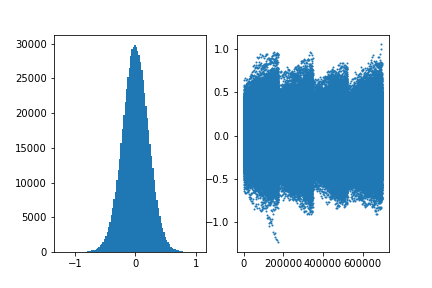
\includegraphics[width=10.5cm]{muestrak.png}
	\caption{Distribución de la traza para una muestra de \texttt{train\_k}.}
    \label{fig:muestrak}
\end{figure}

\subsection*{Modelo de error aditivo (Fair $Add$)}

Crearemos las siguientes funciones para construir el \textit{modelo de error aditivo}:

\begin{itemize}
    \item \texttt{calculate\_eps(dic\_train,dic\_test,var)} :\\ 
    Estima el error $\epsilon$, entrenando el modelo utilizando el conjunto total de datos (\texttt{dic\_train+dic\_test}) para una variable observada \texttt{var} usando además los atributos protegidos. Calculamos los residuos de cada modelo como $$\epsilon_{\texttt{var}} = \texttt{var} - \hat{Y}_\texttt{var}\text{(A)},$$ donde \texttt{var} puede tomar el valor de LSAT o GPA.\\
    \item \texttt{mod\_fair\_add(dic\_train,dic\_test)} :\\
    Estimamos el error para GPA ($\epsilon_\text{GPA}$) y LSAT ($\epsilon_\text{LSAT}$) para el conjunto de entrenamiento (\texttt{dic\_train}) utilizando el método previo. Usamos los valores de $\epsilon_\text{GPA}$ y $\epsilon_\text{LSAT}$ para entrenar el modelo. Finalmente, usaremos el regresor lineal para calcular las predicciones sobre el conjunto de datos de prueba (\texttt{dic\_test}). 
\end{itemize}

\begin{figure}[h]
	\centering
	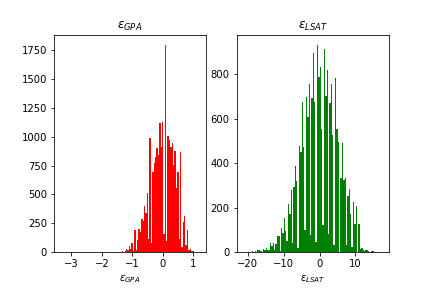
\includegraphics[width=10.5cm]{epsilons.png}
	\caption{Distribución de los residuos calculados para cada variable (GPA y LSAT).}
    \label{fig:epsilondistr}
\end{figure}

\subsection{Exactitud de los modelos}

Para estimar el rendimiento y evaluar el ajuste del modelo, usaremos el error cuadrático medio y el coeficiente de determinación de la predicción (ver su definición en la Sección \ref{sec:coeficientedet}).

En la práctica calcularemos el RMSE haciendo la raíz cuadrada (\texttt{sqrt} de la biblioteca NumPy) a la función \texttt{mean\_squared\_error} sobre los conjuntos de las predicciones de FYA y sus valores reales. Por otro lado, calcularemos el valor de $R^2$, haciendo uso del método \texttt{score} del regresor lineal, sobre los valores y etiquetas reales del conjunto de prueba.

\subsection{Contrafactuales}

Para calcular las distribuciones contrafactuales definiremos las siguientes funciones:

\begin{itemize}
    \item \texttt{cambiar\_individuos(dic, protected\_attr, referencia, objetivo)} :\\
    Realiza una copia (con el método \texttt{deepcopy} del módulo copy) del diccionario \texttt{dic}, cambiando el atributo \texttt{objetivo} perteneciente a los atributos protegidos (\texttt{protected\_attr}) por el valor del \texttt{referencia} para todos los individuos que lo cumplan.\\
    \item \texttt{preds\_individuos(orig\_data, protected\_attr, atributo, preds)} :\\
    Devuelve la restricción del array de predicciones (\texttt{preds}) para el grupo de individuos del conjunto de datos \texttt{orig\_data} que presenten el valor del \texttt{atributo} perteneciente a los atributos protegidos (\texttt{protected\_attr}).\\
    \item \texttt{preds\_array\_individuos(orig\_data, protected\_attr, atributos, preds)} :\\
    Mismo funcionamiento que el anterior, pero para un array de \texttt{atributos}.
\end{itemize}

\section{Contraste de los resultados} \label{sec:contrastresults}

\subsection{Actuación de los modelos}

En un modelo de regresión, el objetivo es predecir el valor numérico de una cantidad desconocida a partir de unas características dadas. Llamaremos error de predicción a la diferencia entre la predicción y el valor real. Usaremos como medida de evaluación el error cuadrático medio (RMSE), que indica cómo de cerca están los valores observados de los valores predichos por el modelo. Si comparamos el RMSE entre dos modelos, un valor más bajo indicará un mejor ajuste de los datos.

También usaremos el coeficiente de determinación ($R^2$), que refleja la bondad del ajuste de un modelo a la variable que pretende explicar. El resultado del coeficiente de determinación oscila entre 0 y 1. Cuánto más cerca de 1 se sitúe su valor, mejor será el ajuste del modelo. Por el contrario, cuánto más cerca de cero, menos ajustado estará el modelo y, por tanto, será menos fiable.\\

\begin{table}[h]
\centering
\resizebox{12.1cm}{!} {
\begin{tabular}{ccccc}
\hline
      & \textbf{Completo} & \textbf{Desconocimiento} & \textbf{Fair $K$} & \textbf{Fair Add} \\ \hline
RMSE  & 0.8720         & 0.8916                   & 0.9312            & 0.9191            \\ \hline
$R^2$ & 0.8560        & 0.8949                   & 0.9761            & 0.9510            \\ \hline
\end{tabular}
}
\caption{Valores de RMSE y $R^2$ para los cuatro modelos.}
\label{tab:coeficientes}
\end{table}\

Comparamos el RMSE alcanzado por la regresión lineal sobre el conjunto de prueba para cada modelo en la Tabla \ref{tab:coeficientes}. El modelo completo obtiene el RMSE más bajo, ya que utiliza mayor número de atributos para reconstruir con mayor precisión el valor de FYA. El modelo por desconocimiento usa las variables injustas GPA y LSAT, pero como no utiliza las variables raza y sexo, un menor número de atributos, hace que no pueda igualar el RMSE del modelo completo. Los modelos Fair $K$ y Fair $Add$, al satisfacer la equidad contrafactual, compensan algo de exactitud. El modelo Fair $K$ utiliza supuestos más débiles, y por tanto, el RMSE es más elevado. Por otro lado, usando los supuestos del modelo Fair $Add$, producimos un modelo justo contrafactualmente, que sacrifica suposiciones ligeramente más fuertes por un RMSE más bajo. 

%MODIFICAR
Respecto a $R^2$, el modelo con un mejor valor es el modelo completo, que como ya hemos explicado previamente, al utilizar todas los atributos existentes, obtiene mejores resultados en su predicción. Aún así, el modelo completo no obtiene un $R^2$ muy bueno, teniendo en cuenta que este valor se encuentra en el intervalo [0,1], siendo 1 el ajuste perfecto del modelo. Los peores valores de $R^2$ lo consiguen el nivel 2 y 3, obteniendo unas predicciones bastante deficientes, comparándolas con los valores reales de FYA.

\subsection{Estudio de la equidad}

A continuación, utilizaremos los escenarios propuestos para realizar un estudio de la equidad sobre los diferentes aspectos estudiados en la teoría. 

Realizaremos un cálculo de los contrafactuales basándonos en el escenario del nivel 2, y visualizaremos gráficamente el cambio en la distribución de los individuos cuando modificamos sus atributos. Por otro lado, presentaremos un estudio en Aequitas sobre las nociones de equidad, que cumplen los datos bajo las predicciones de los cuatro modelos estudiados.

\subsubsection{Distribuciones contrafactuales} \label{subsec:graficas}

Comprobaremos empíricamente si los modelos propuestos son justos desde el punto de vista contrafactual. Para ello, supondremos que el modelo real del mundo viene dado por la Figura \ref{fig:nivel2solo}, que corresponde con el modelo de variable latente (Fair $K$). Podemos ajustar los parámetros de este modelo utilizando los datos observados, y evaluar la equidad contrafactual mediante un muestreo del mismo. 

Generaremos muestras para los atributos de raza y sexo a partir de las variables observadas y las variables contrafactuales. Ajustaremos los modelos tanto a la muestra original como a la contrafactual, y pintaremos una gráfica (usando la función \texttt{displot}) mostrando los cambios en la distribución de la FYA predicha para ambos modelos de referencia.\\

\begin{figure}[h]
	\centering
	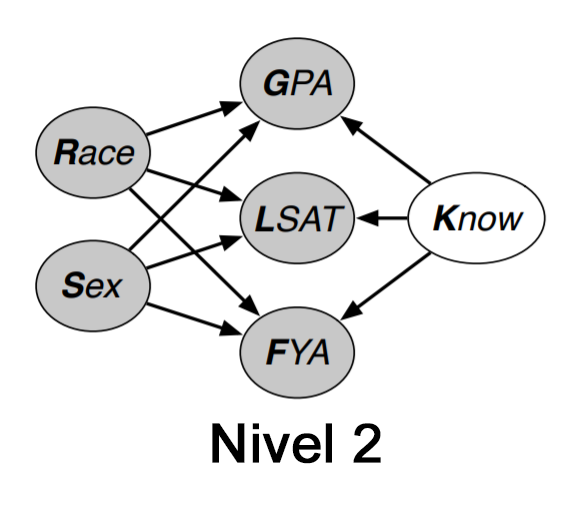
\includegraphics[width=5.5cm]{nivel2grafo.png}
	\caption{Grafo causal del escenario propuesto para el nivel 2.}
    \label{fig:nivel2solo}
\end{figure}

En la Tabla \ref{tab:procesocontrafact}, visualizamos un ejemplo del cálculo del contrafactual sobre un individuo seleccionado aleatoriamente en la población. En nuestro caso, hemos escogido un individuo de la población con los atributos de \textit{sexo}=mujer y \textit{raza}=asiática, con unos valores determinados de GPA, LSAT y FYA (para simplificar, tomarán valores binarios (\textit{fail}/\textit{ok})). Para que el modelo cumpla la equidad contrafactual, la decisión predicha, debe ser igual a la predicción sobre el mismo individuo con un cambio en uno de sus atributos protegidos. Normalmente el cambio se realiza de un valor objetivo por su valor de referencia.\\

\begin{table}[h]
\centering
\resizebox{16.1cm}{!} {
\begin{tabular}{ccccclcccccc}
\cline{1-5} \cline{7-12}
\multicolumn{5}{|c|}{1. Seleccionar un individuo:}                                                                                                                                                                       & \multicolumn{1}{l|}{}          & \multicolumn{6}{c|}{3. Calcular la variable $K$ no observada del modelo causal:}                                                                                                                                                                                                      \\ \cline{1-5} \cline{7-12} 
\multicolumn{1}{|c|}{$A_S$} & \multicolumn{1}{c|}{$A_R$}          & \multicolumn{1}{c|}{GPA}                         & \multicolumn{1}{c|}{LSAT}                      & \multicolumn{1}{c|}{FYA}                         & \multicolumn{1}{l|}{\textbf{}} & \multicolumn{1}{c|}{a'} & \multicolumn{1}{c|}{$A_R$}             & \multicolumn{1}{c|}{GPA}                         & \multicolumn{1}{c|}{LSAT}                      & \multicolumn{1}{c|}{FYA}                         & \multicolumn{1}{c|}{$K$}                       \\ \cline{1-5} \cline{7-12} 
\multicolumn{1}{|c|}{female}  & \multicolumn{1}{c|}{asian}          & \multicolumn{1}{c|}{{\color[HTML]{FE0000} FAIL}} & \multicolumn{1}{c|}{{\color[HTML]{32CB00} OK}} & \multicolumn{1}{c|}{{\color[HTML]{FE0000} FAIL}} & \multicolumn{1}{l|}{}          & \multicolumn{1}{c|}{\textbf{male}}  & \multicolumn{1}{c|}{asian} & \multicolumn{1}{c|}{{\color[HTML]{FE0000} FAIL}} & \multicolumn{1}{c|}{{\color[HTML]{32CB00} OK}} & \multicolumn{1}{c|}{{\color[HTML]{FE0000} FAIL}} & \multicolumn{1}{c|}{{\color[HTML]{32CB00} OK}} \\ \cline{1-5} \cline{7-12} 
\multicolumn{1}{l}{}        & \multicolumn{1}{l}{}                & \multicolumn{1}{l}{}                             & \multicolumn{1}{l}{}                           & \multicolumn{1}{l}{}                             &                                & \multicolumn{1}{l}{}       & \multicolumn{1}{l}{}                & \multicolumn{1}{l}{}                             & \multicolumn{1}{l}{}                           & \multicolumn{1}{l}{}                             & \multicolumn{1}{l}{}                           \\ \cline{1-5} \cline{7-12} 
\multicolumn{5}{|c|}{2. Cambiar el valor del atributo protegido:}                                                                                                                                                        & \multicolumn{1}{l|}{}          & \multicolumn{6}{c|}{4. Recalcular las variables observadas del modelo causal:}                                                                                                                                                                                                      \\ \cline{1-5} \cline{7-12} 
\multicolumn{1}{|c|}{a'} & \multicolumn{1}{c|}{$A_R$}             & \multicolumn{1}{c|}{GPA}                         & \multicolumn{1}{c|}{LSAT}                      & \multicolumn{1}{c|}{FYA}                         & \multicolumn{1}{c|}{}          & \multicolumn{1}{c|}{a'} & \multicolumn{1}{c|}{$A_R$}             & \multicolumn{1}{c|}{GPA$_{A_S\leftarrow a'}$}      & \multicolumn{1}{c|}{LSAT$_{A_S\leftarrow a'}$}    & \multicolumn{1}{c|}{FYA$_{A_S\leftarrow a'}$}      & \multicolumn{1}{c|}{$K$}                       \\ \cline{1-5} \cline{7-12} 
\multicolumn{1}{|c|}{\textbf{male}}  & \multicolumn{1}{c|}{asian} & \multicolumn{1}{c|}{{\color[HTML]{FE0000} FAIL}} & \multicolumn{1}{c|}{{\color[HTML]{32CB00} OK}} & \multicolumn{1}{c|}{{\color[HTML]{FE0000} FAIL}} & \multicolumn{1}{l|}{}          & \multicolumn{1}{c|}{\textbf{male}}  & \multicolumn{1}{c|}{asian} & \multicolumn{1}{c|}{{\color[HTML]{32CB00} OK}}   & \multicolumn{1}{c|}{{\color[HTML]{32CB00} OK}} & \multicolumn{1}{c|}{{\color[HTML]{32CB00} OK}}   & \multicolumn{1}{c|}{{\color[HTML]{32CB00} OK}} \\ \cline{1-5} \cline{7-12} 
\end{tabular}
}
\caption{Proceso de cálculo de contrafactual sobre un individuo para la variable $K$.}
\label{tab:procesocontrafact}
\end{table}

En el ejemplo de la Tabla \ref{tab:procesocontrafact}, realizamos el cálculo del contrafactual para el atributo sexo, por lo que cambiamos el valor \textit{female} por \textit{male} (históricamente considerado más aventajado). Una vez cambiado el valor del atributo para el individuo, calcularemos el valor de la variable no observada $K$, que en nuestro caso, se calcula siguiendo el modelo Fair $K$. Finalmente, eliminamos los valores restantes y predecimos estos valores (en este problema, solo nos interesa el valor de FYA) a partir del nuevo valor de $K$. Como podemos observar; el valor de FYA ha cambiado, por lo que para este individuo, el modelo utilizado en la predicción, no sería justo contrafactualmente para el atributo protegido sexo.

\clearpage

Replicaremos el proceso de la Tabla \ref{tab:procesocontrafact} para todos los individuos del \textit{dataset}. Los cambios en los atributos se harán usando el método \texttt{cambiar\_individuos} implementado. La Figura \ref{fig:grafofull} muestra el cambio de las distribuciones contrafactuales usando el modelo completo, donde cada columna corresponde al cambio contrafactual para el atributo específico. La Figura \ref{fig:grafoware} muestra lo mismo, pero para el modelo por desconocimiento. En cada gráfica, la distribución azul muestra la densidad de los datos originales y la distribución roja la de los datos contrafactuales. Si un modelo es contrafactualmente justo, estas distribuciones serán lo más parecidas posibles. Cabe destacar que la gráfica en cada columna representa la distribución condicionada a los dos grupos de individuos indicados, para ello usamos la función \texttt{preds\_array\_individuos}.\\

\begin{figure}[h]
	\centering
	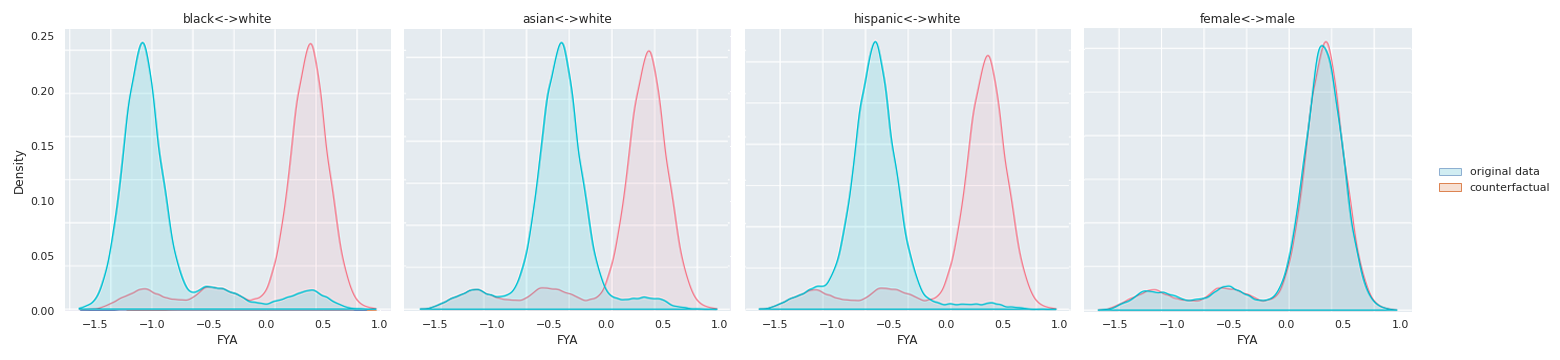
\includegraphics[width=16.8cm]{grafofull.png}
	\caption{Distribución contrafactual para el modelo completo.}
    \label{fig:grafofull}
\end{figure}

En la Figura \ref{fig:grafofull}, vemos que el modelo es injusto para los tres valores de los atributos más comunes de raza (black, asian, hispanic), mientras que es justo contrafactualmente para el atributo sexo.\\

\begin{figure}[h]
	\centering
	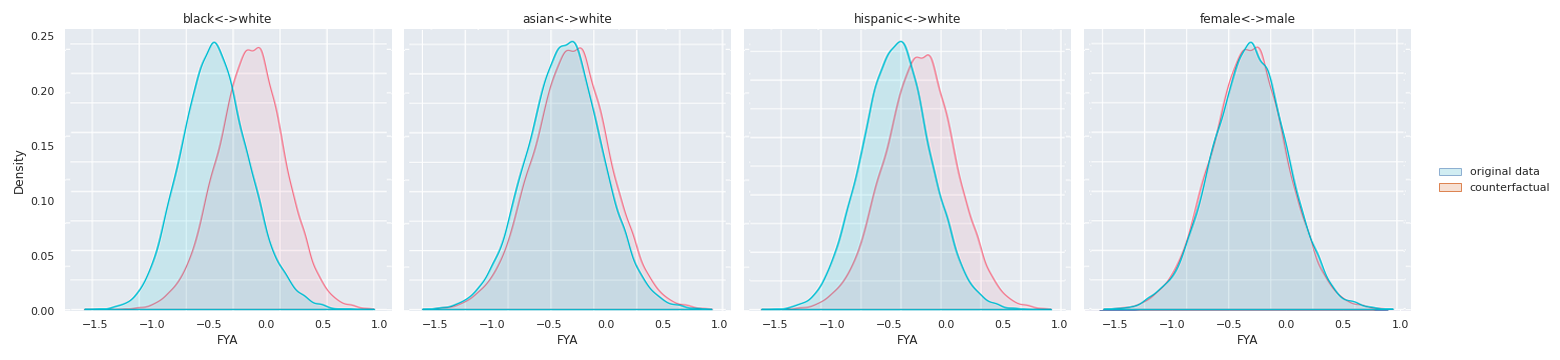
\includegraphics[width=16.8cm]{grafoware.png}
	\caption{Distribución contrafactual para el modelo por desconocimiento.}
    \label{fig:grafoware}
\end{figure}

La Figura \ref{fig:grafoware} obtiene resultados a primera vista más justos para los atributos de raza. En nuestro caso, la raza asiática se podría considerar justa contrafactualmente para este modelo. Al igual que para el modelo completo, el atributo sexo no parece estar sesgado en este problema. Haciendo la media de los pesos para todos los individuos masculinos y femeninos obtenemos un valor de (0.91, 1.03) para GPA y (0.98,0.99) para LSAT. Concluimos que estos modelos son justos con respecto al sexo, ya que existe una relación causal muy débil entre el atributo sexo y los atributos GPA y LSAT.

\subsubsection{Análisis extendido en Aequitas}

Definiremos las siguientes funciones, que nos ayudarán a convertir el array de predicciones calculadas por cada modelo, a una estructura de datos tratable por Aequitas:

\begin{itemize}
    \item \texttt{get\_aequitas\_data(train\_orig, preds\_train, test\_orig, preds\_test)} :\\
    Construye un \textit{dataset} utilizando los valores originales de \textit{raza, sexo} y \textit{first\_pf} (contenidos en \texttt{train\_orig} y \texttt{test\_orig}) y guarda como \textit{score} las nuevas predicciones \texttt{preds\_train} y \texttt{preds\_test} para el modelo en cuestión. Finalmente, concatena ambos subconjuntos y define la estructura compatible con Aequitas definida en el Apéndice \ref{ap:herr_just}.\\
    \item \texttt{save\_graficas(data, path, aq\_palette, attr)} :\\
    Genera gráficas de distribución del atributo \texttt{attr} para un conjunto de datos (\texttt{data}). Utiliza el color determinado en \texttt{aq\_palette} y guarda la imagen en la ruta especificada por \texttt{path}.\\
    \item \texttt{tabla\_metrica\_grupo(data)} :\\
    Utiliza la clase \textit{Group()} de Aequitas, para construir la tabla de las métricas de grupo para el conjunto de datos (\texttt{data}).\\
    \item \texttt{tabla\_metrica\_sesgo(data, attr\_ref)} :\\
    Utiliza la clase \textit{Bias()} de Aequitas, para construir la tabla de las métricas de sesgo para el conjunto de datos (\texttt{data}). El parámetro \texttt{attr\_ref} especificará los valores del grupo de referencia.\\
    \item \texttt{tabla\_medidas\_equidad(data, attr\_ref, tau=0.8)} :\\
    Utiliza la clase \textit{Fairness()} de Aequitas, para construir la tabla de las medidas de equidad para el conjunto de datos (\texttt{data}). El parámetro \texttt{attr\_ref} indicará los valores del grupo de referencia y el valor de \texttt{tau}, por defecto 0.8, especificará el umbral tomado para la regla p\%.\\
\end{itemize}

En este apartado, haremos una selección de las métricas de grupo que nos serán útiles para comparar las diferentes nociones de equidad estudiadas, a saber:

\begin{itemize}
    \item \textbf{Paridad estadística} - Aequitas utiliza la tasa de positivos predichos (PPR).
    \item \textbf{Probabilidades igualadas} - Cumplir simultáneamente las métricas asociadas a las tasas de falsos y verdaderos positivos (FPR y TPR, respectivamente).
    \item \textbf{Tasa de paridad predictiva} - Cumplir simultáneamente los valores positivo y negativo predictivo (PPV y NPV, respectivamente). En Aequitas el PPV se registra por su otro nombre: precision.
    \clearpage
    \item \textbf{Paridad tipo II} - Al encontrarnos con un problema de tipo asistencial, podría ser relevante el estudio de esta medida de equidad. Esta medida se cumple cuando se aceptan como justas simultáneamente las métricas relativas a la tasa de falsa omisión (FOR) y falsos negativos (FNR).
\end{itemize}

El objetivo de este apartado, es comprobar si la actuación de los modelos justos, favorecen el cumplimiento de otras métricas de grupo, las cuales hemos estudiado en teoría. El análisis se reducirá a hacer un estudio de las tablas de métricas de grupo, sesgo y finalmente estudiar para qué casos se cumple una medida de equidad u otra. Un análisis sobre los conjuntos de datos originales para \textit{law\_data} y \textit{COMPAS}, profundizando en otras métricas y las herramientas gráficas que ofrece Aequitas, podrá encontrarse en el Apéndice \ref{ap:herr_just}.

Presentaremos para cada modelo: la distribución de sus puntuaciones predichas, su tabla de métricas de grupo y sesgo, y las medidas de equidad que cumplen. Finalmente, haremos un contraste general de los resultados para los cuatro modelos.

\subsubsection*{Modelo completo}

Comparando las distribuciones de las predicciones (\textit{score}) con las etiquetas reales (\textit{label\_value}), vemos que en la Figura \ref{fig:scorefull}, la actuación del modelo completo, a primera vista, tiene unos resultados injustos en términos de equidad respecto al atributo raza. Mientras que las puntuaciones de los individuos de raza blanca, son muy similares a los de la etiqueta real, las puntuaciones favorables hacia individuos de otra raza son mínimas o inexistentes.\\

\begin{figure}[h]
    \minipage{0.53\textwidth}
      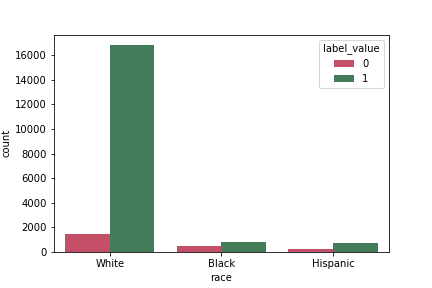
\includegraphics[width=\linewidth]{images/label_race_law_2.png}
    \endminipage\hfill
    \minipage{0.53\textwidth}%
      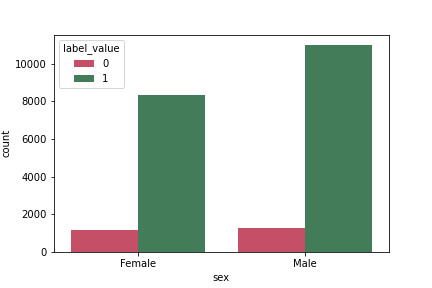
\includegraphics[width=\linewidth]{images/label_sex_law_2.png}
    \endminipage
     \caption{Distribución de las etiquetas reales para los atributos protegidos.}
     \label{fig:labelracesex3}
\end{figure}

\clearpage

El modelo completo era el que mejores resultados de RMSE y $R^2$ ofrecía, esto se debe a que al entrenar con todos los atributos, favorece la predicción correcta para los individuos de la clase mayoritaria (raza blanca), mientras que los individuos de grupos desfavorecidos obtienen resultados nefastos en la regresión realizada.

\begin{figure}[h]
    \minipage{0.53\textwidth}
      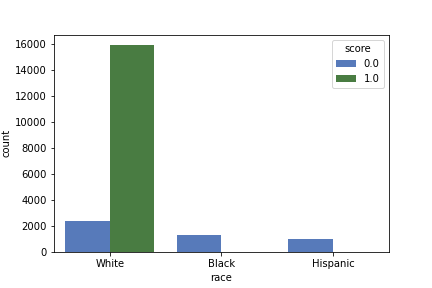
\includegraphics[width=\linewidth]{images/score_full_race_law.png}
    \endminipage\hfill
    \minipage{0.53\textwidth}%
      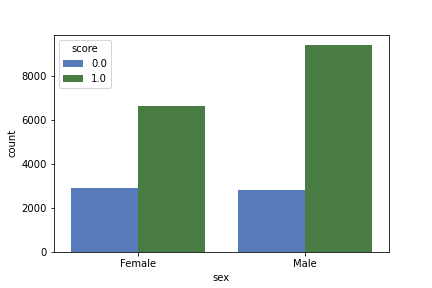
\includegraphics[width=\linewidth]{images/score_full_sex_law.png}
    \endminipage
     \caption{Distribución de la puntuación para el modelo completo.}
     \label{fig:scorefull}
\end{figure}

Definiremos las tablas para las métricas de grupo (Tabla \ref{tab:grupofull}) y sesgo (Tabla \ref{tab:sesgofull}) calculadas con las predicciones de este modelo. Además, también aportaremos una tabla, indicando el cumplimiento o no de las nociones de equidad (Tabla \ref{tab:equidadfull}) sobre las que nos hemos centrado.\\

\begin{table}[h]
\centering
\resizebox{13.cm}{!} {
\begin{tabular}{|c|c|c|c|c|c|c|c|c|}
\hline
\textbf{\begin{tabular}[c]{@{}c@{}}Nombre\\ del Atributo\end{tabular}} & \textbf{\begin{tabular}[c]{@{}c@{}}Valor\end{tabular}} & \textbf{PPR} & \textbf{FPR} & \textbf{TPR} & \textbf{PPV} & \textbf{NPV} & \textbf{FOR} & \textbf{FNR} \\ \hline
\textbf{race}                                                     & Asian                                                              & 0.0          & 0.01         & 0.11         & 0.97         & 0.20         & 0.80         & 0.89         \\ \hline
\textbf{race}                                                     & Black                                                              & 0.0          & 0.0          & 0.0          & -            & 0.38         & 0.62         & 1.0          \\ \hline
\textbf{race}                                                     & Hispanic                                                           & 0.0          & 0.0          & 0.03         & 0.95         & 0.26         & 0.74         & 0.97         \\ \hline
\textbf{race}                                                     & Other                                                              & 0.0          & 0.01         & 0.24         & 0.99         & 0.25         & 0.75         & 0.76         \\ \hline
\textbf{race}                                                     & White                                                              & 0.99         & 0.66         & 0.89         & 0.94         & 0.21         & 0.79         & 0.11         \\ \hline
\textbf{sex}                                                      & Female                                                             & 0.41         & 0.34         & 0.75         & 0.94         & 0.27         & 0.73         & 0.25         \\ \hline
\textbf{sex}                                                      & Male                                                               & 0.59         & 0.45         & 0.81         & 0.94         & 0.24         & 0.76         & 0.19         \\ \hline
\end{tabular}
}
\caption{Métricas de grupo para el modelo completo.}
\label{tab:grupofull}
\end{table}

Para las métricas de sesgo, trataremos como atributos de referencia la raza blanca y el sexo masculino. Además, utilizaremos el criterio de la regla del 80\%, por lo que los valores de la tabla de métricas de sesgo que no estén definidas en el intervalo [0.8,1.25] serán consideradas como injustas y coloreadas en rojo, mientras que los valores contenidos en el intervalo vendrán indicados en verde. Para el resto de modelos, mantendremos el mismo valor de umbral (80\%), y mantendremos la acepción del coloreado para la tabla de métricas de sesgo.\\

\begin{table}[h]
\centering
\resizebox{16.cm}{!} {
\begin{tabular}{|c|c|c|c|c|c|c|c|c|}
\hline
\textbf{\begin{tabular}[c]{@{}c@{}}Nombre\\ del Atributo\end{tabular}} & \textbf{\begin{tabular}[c]{@{}c@{}}Valor\end{tabular}} & \textbf{\begin{tabular}[c]{@{}c@{}}PPR\\ Disparity\end{tabular}} & \textbf{\begin{tabular}[c]{@{}c@{}}FPR\\ Disparity\end{tabular}} & \textbf{\begin{tabular}[c]{@{}c@{}}TPR\\ Disparity\end{tabular}} & \textbf{\begin{tabular}[c]{@{}c@{}}PPV\\ Disparity\end{tabular}} & \textbf{\begin{tabular}[c]{@{}c@{}}NPV\\ Disparity\end{tabular}} & \textbf{\begin{tabular}[c]{@{}c@{}}FOR\\ Disparity\end{tabular}} & \textbf{\begin{tabular}[c]{@{}c@{}}FNR\\ Disparity\end{tabular}} \\ \hline
\textbf{race}                                                     & Asian                                                              & {\color[HTML]{FE0000} 0.0}                                       & {\color[HTML]{FE0000} 0.02}                                      & {\color[HTML]{FE0000} 0.12}                                      & {\color[HTML]{32CB00} 1.03}                                      & {\color[HTML]{32CB00} 0.95}                                      & {\color[HTML]{32CB00} 1.01}                                      & {\color[HTML]{FE0000} 8.09}                                      \\ \hline
\textbf{race}                                                     & Black                                                              & {\color[HTML]{FE0000} 0.0}                                       & {\color[HTML]{FE0000} 0.0}                                       & {\color[HTML]{FE0000} 0.0}                                       & {-}                                         & {\color[HTML]{FE0000} 1.81}                                      & {\color[HTML]{FE0000} 0.78}                                      & {\color[HTML]{FE0000} 9.09}                                      \\ \hline
\textbf{race}                                                     & Hispanic                                                           & {\color[HTML]{FE0000} 0.0}                                       & {\color[HTML]{FE0000} 0.0}                                       & {\color[HTML]{FE0000} 0.03}                                      & {\color[HTML]{32CB00} 1.01}                                      & {\color[HTML]{32CB00} 1.24}                                      & {\color[HTML]{32CB00} 0.94}                                      & {\color[HTML]{FE0000} 8.82}                                      \\ \hline
\textbf{race}                                                     & Other                                                              & {\color[HTML]{FE0000} 0.0}                                       & {\color[HTML]{FE0000} 0.02}                                      & {\color[HTML]{FE0000} 0.27}                                      & {\color[HTML]{32CB00} 1.05}                                      & {\color[HTML]{32CB00} 1.19}                                      & {\color[HTML]{32CB00} 0.95}                                      & {\color[HTML]{FE0000} 6.91}                                      \\ \hline
\textbf{race}                                                     & White                                                              & {\color[HTML]{3166FF} 1.0}                                       & {\color[HTML]{3166FF} 1.0}                                       & {\color[HTML]{3166FF} 1.0}                                       & {\color[HTML]{3166FF} 1.0}                                       & {\color[HTML]{3166FF} 1.0}                                       & {\color[HTML]{3166FF} 1.0}                                       & {\color[HTML]{3166FF} 1.0}                                       \\ \hline
\textbf{sex}                                                      & Female                                                             & {\color[HTML]{FE0000} 0.69}                                      & {\color[HTML]{FE0000} 0.76}                                      & {\color[HTML]{32CB00} 0.93}                                      & {\color[HTML]{32CB00} 1.0}                                       & {\color[HTML]{32CB00} 1.13}                                      & {\color[HTML]{32CB00} 0.96}                                      & {\color[HTML]{FE0000} 1.32}                                      \\ \hline
\textbf{sex}                                                      & Male                                                               & {\color[HTML]{3166FF} 1.0}                                       & {\color[HTML]{3166FF} 1.0}                                       & {\color[HTML]{3166FF} 1.0}                                       & {\color[HTML]{3166FF} 1.0}                                       & {\color[HTML]{3166FF} 1.0}                                       & {\color[HTML]{3166FF} 1.0}                                       & {\color[HTML]{3166FF} 1.0}                                       \\ \hline
\end{tabular}
}
\caption{Métricas de sesgo para el modelo completo.}
\label{tab:sesgofull}
\end{table}

\begin{table}[h]
\centering
\resizebox{15.5cm}{!} {
\begin{tabular}{|c|c|c|c|c|c|c|c|}
\hline
\textbf{\begin{tabular}[c]{@{}c@{}}Nombre\\ del Atributo\end{tabular}} & \textbf{\begin{tabular}[c]{@{}c@{}}PPR\\ Disparity\end{tabular}} & \textbf{\begin{tabular}[c]{@{}c@{}}FPR\\ Disparity\end{tabular}} & \textbf{\begin{tabular}[c]{@{}c@{}}TPR\\ Disparity\end{tabular}} & \textbf{\begin{tabular}[c]{@{}c@{}}PPV\\ Disparity\end{tabular}} & \textbf{\begin{tabular}[c]{@{}c@{}}NPV\\ Disparity\end{tabular}} & \textbf{\begin{tabular}[c]{@{}c@{}}FOR\\ Disparity\end{tabular}} & \textbf{\begin{tabular}[c]{@{}c@{}}FNR\\ Disparity\end{tabular}} \\ \hline
\textbf{race}                                                     & {\color[HTML]{FE0000} FALSE}                                     & {\color[HTML]{FE0000} FALSE}                                     & {\color[HTML]{FE0000} FALSE}                                     & {\color[HTML]{32CB00} TRUE}                                      & {\color[HTML]{FE0000} FALSE}                                     & {\color[HTML]{FE0000} FALSE}                                     & {\color[HTML]{FE0000} FALSE}                                     \\ \hline
\textbf{sex}                                                      & {\color[HTML]{FE0000} FALSE}                                     & {\color[HTML]{FE0000} FALSE}                                     & {\color[HTML]{32CB00} TRUE}                                      & {\color[HTML]{32CB00} TRUE}                                      & {\color[HTML]{32CB00} TRUE}                                      & {\color[HTML]{32CB00} TRUE}                                      & {\color[HTML]{FE0000} FALSE}                                     \\ \hline
\end{tabular}
}
\caption{Medidas de equidad para el modelo completo.}
\label{tab:equidadfull}
\end{table}


\subsubsection*{Modelo por desconocimiento}

Para este modelo, la predicción de la puntuación para los individuos de las clases minoritarias sufre cierta mejoría respecto al modelo completo analizado anteriormente.

En la Figura \ref{fig:scoreunaware} podemos observar cómo ya existen algunos individuos de otras razas que obtienen una puntuación favorable. Esto se debe a que no tenemos en cuenta los atributos protegidos en la predicción. No obstante, probablemente sigan existiendo sesgos entre los diferentes grupos demográficos existentes. El modelo por desconocimiento también favorece la clasificación negativa (\textit{score}=0) de individuos por sexo, en comparación con el modelo anterior.\\

\begin{figure}[H]
    \minipage{0.53\textwidth}
      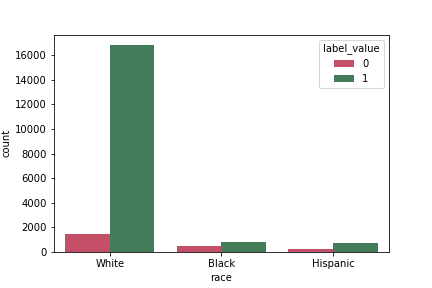
\includegraphics[width=\linewidth]{images/label_race_law_2.png}
    \endminipage\hfill
    \minipage{0.53\textwidth}%
      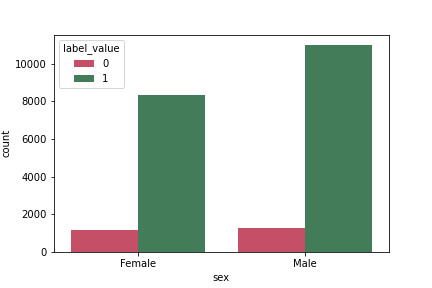
\includegraphics[width=\linewidth]{images/label_sex_law_2.png}
    \endminipage
     \caption{Distribución de las etiquetas reales para los atributos protegidos.}
     \label{fig:labelracesex4}
\end{figure}

\begin{figure}[H]
    \minipage{0.53\textwidth}
      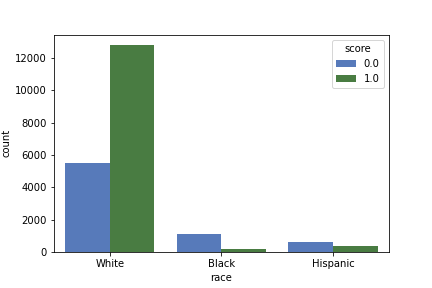
\includegraphics[width=\linewidth]{images/score_unaware_race_law.png}
    \endminipage\hfill
    \minipage{0.53\textwidth}%
      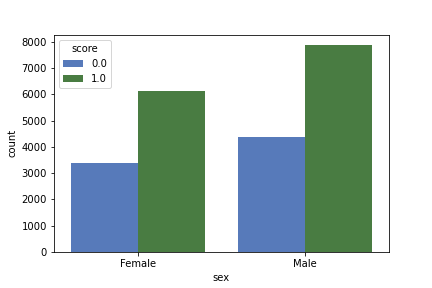
\includegraphics[width=\linewidth]{images/score_unaware_sex_law.png}
    \endminipage
     \caption{Distribución de la puntuación para el modelo por desconocimiento.}
     \label{fig:scoreunaware}
\end{figure}

A continuación definimos las tablas para las métricas de grupo (Tabla \ref{tab:grupounaware}) y sesgo (Tabla \ref{tab:sesgounaware}) calculadas con las predicciones de este modelo. También presentamos la tabla con las medidas de equidad (Tabla \ref{tab:equidadunaware}) para este modelo concreto.\\

\begin{table}[H]
\centering
\resizebox{13.cm}{!} {
\begin{tabular}{|c|c|c|c|c|c|c|c|c|}
\hline
\textbf{\begin{tabular}[c]{@{}c@{}}Nombre\\ del Atributo\end{tabular}} & \textbf{\begin{tabular}[c]{@{}c@{}}Valor\end{tabular}} & \textbf{PPR} & \textbf{FPR} & \textbf{TPR} & \textbf{PPV} & \textbf{NPV} & \textbf{FOR} & \textbf{FNR} \\ \hline
\textbf{race}                                                     & Asian                                                              & 0.03         & 0.35         & 0.63         & 0.89         & 0.29         & 0.71         & 0.37         \\ \hline
\textbf{race}                                                     & Black                                                              & 0.01         & 0.04         & 0.19         & 0.89         & 0.42         & 0.58         & 0.81         \\ \hline
\textbf{race}                                                     & Hispanic                                                           & 0.03         & 0.16         & 0.45         & 0.89         & 0.34         & 0.66         & 0.55         \\ \hline
\textbf{race}                                                     & Other                                                              & 0.01         & 0.23         & 0.58         & 0.91         & 0.32         & 0.68         & 0.42         \\ \hline
\textbf{race}                                                     & White                                                              & 0.91         & 0.43         & 0.72         & 0.95         & 0.15         & 0.85         & 0.28         \\ \hline
\textbf{sex}                                                      & Female                                                             & 0.44         & 0.28         & 0.70         & 0.95         & 0.25         & 0.75         & 0.30         \\ \hline
\textbf{sex}                                                      & Male                                                               & 0.56         & 0.34         & 0.68         & 0.95         & 0.19         & 0.81         & 0.32         \\ \hline
\end{tabular}
}
\caption{Métricas de grupo para el modelo por desconocimiento.}
\label{tab:grupounaware}
\end{table}

\begin{table}[H]
\centering
\resizebox{16.cm}{!} {
\begin{tabular}{|c|c|c|c|c|c|c|c|c|}
\hline
\textbf{\begin{tabular}[c]{@{}c@{}}Nombre\\ del Atributo\end{tabular}} & \textbf{\begin{tabular}[c]{@{}c@{}}Valor\end{tabular}} & \textbf{\begin{tabular}[c]{@{}c@{}}PPR\\ Disparity\end{tabular}} & \textbf{\begin{tabular}[c]{@{}c@{}}FPR\\ Disparity\end{tabular}} & \textbf{\begin{tabular}[c]{@{}c@{}}TPR\\ Disparity\end{tabular}} & \textbf{\begin{tabular}[c]{@{}c@{}}PPV\\ Disparity\end{tabular}} & \textbf{\begin{tabular}[c]{@{}c@{}}NPV\\ Disparity\end{tabular}} & \textbf{\begin{tabular}[c]{@{}c@{}}FOR\\ Disparity\end{tabular}} & \textbf{\begin{tabular}[c]{@{}c@{}}FNR\\ Disparity\end{tabular}} \\ \hline
\textbf{race}                                                     & Asian                                                              & {\color[HTML]{FE0000} 0.03}                                      & {\color[HTML]{32CB00} 0.81}                                      & {\color[HTML]{32CB00} 0.88}                                      & {\color[HTML]{32CB00} 0.94}                                      & {\color[HTML]{32CB00} 1.93}                                      & {\color[HTML]{32CB00} 0.84}                                      & {\color[HTML]{FE0000} 1.32}                                      \\ \hline
\textbf{race}                                                     & Black                                                              & {\color[HTML]{FE0000} 0.01}                                      & {\color[HTML]{FE0000} 0.09}                                      & {\color[HTML]{FE0000} 0.26}                                      & {\color[HTML]{32CB00} 0.94}                                      & {\color[HTML]{FE0000} 2.8}                                       & {\color[HTML]{FE0000} 0.68}                                      & {\color[HTML]{FE0000} 2.89}                                      \\ \hline
\textbf{race}                                                     & Hispanic                                                           & {\color[HTML]{FE0000} 0.03}                                      & {\color[HTML]{FE0000} 0.37}                                      & {\color[HTML]{FE0000} 0.63}                                      & {\color[HTML]{32CB00} 0.94}                                      & {\color[HTML]{FE0000} 2.27}                                      & {\color[HTML]{FE0000} 0.78}                                      & {\color[HTML]{FE0000} 1.96}                                      \\ \hline
\textbf{race}                                                     & Other                                                              & {\color[HTML]{FE0000} 0.01}                                      & {\color[HTML]{FE0000} 0.53}                                      & {\color[HTML]{32CB00} 0.81}                                      & {\color[HTML]{32CB00} 0.96}                                      & {\color[HTML]{FE0000} 2.13}                                      & {\color[HTML]{32CB00} 0.8}                                       & {\color[HTML]{FE0000} 1.5}                                       \\ \hline
\textbf{race}                                                     & White                                                              & {\color[HTML]{3166FF} 1.0}                                       & {\color[HTML]{3166FF} 1.0}                                       & {\color[HTML]{3166FF} 1.0}                                       & {\color[HTML]{3166FF} 1.0}                                       & {\color[HTML]{3166FF} 1.0}                                       & {\color[HTML]{3166FF} 1.0}                                       & {\color[HTML]{3166FF} 1.0}                                       \\ \hline
\textbf{sex}                                                      & Female                                                             & {\color[HTML]{FE0000} 0.79}                                      & {\color[HTML]{32CB00} 0.82}                                      & {\color[HTML]{32CB00} 1.03}                                      & {\color[HTML]{32CB00} 1.0}                                       & {\color[HTML]{FE0000} 1.32}                                      & {\color[HTML]{32CB00} 0.93}                                      & {\color[HTML]{32CB00} 0.94}                                      \\ \hline
\textbf{sex}                                                      & Male                                                               & {\color[HTML]{3166FF} 1.0}                                       & {\color[HTML]{3166FF} 1.0}                                       & {\color[HTML]{3166FF} 1.0}                                       & {\color[HTML]{3166FF} 1.0}                                       & {\color[HTML]{3166FF} 1.0}                                       & {\color[HTML]{3166FF} 1.0}                                       & {\color[HTML]{3166FF} 1.0}                                       \\ \hline
\end{tabular}
}
\caption{Métricas de sesgo para el modelo por desconocimiento.}
\label{tab:sesgounaware}
\end{table}

\clearpage

\begin{table}[h]
\centering
\resizebox{15.5cm}{!} {
\begin{tabular}{|c|c|c|c|c|c|c|c|}
\hline
\textbf{\begin{tabular}[c]{@{}c@{}}Nombre\\ del Atributo\end{tabular}} & \textbf{\begin{tabular}[c]{@{}c@{}}PPR\\ Disparity\end{tabular}} & \textbf{\begin{tabular}[c]{@{}c@{}}FPR\\ Disparity\end{tabular}} & \textbf{\begin{tabular}[c]{@{}c@{}}TPR\\ Disparity\end{tabular}} & \textbf{\begin{tabular}[c]{@{}c@{}}PPV\\ Disparity\end{tabular}} & \textbf{\begin{tabular}[c]{@{}c@{}}NPV\\ Disparity\end{tabular}} & \textbf{\begin{tabular}[c]{@{}c@{}}FOR\\ Disparity\end{tabular}} & \textbf{\begin{tabular}[c]{@{}c@{}}FNR\\ Disparity\end{tabular}} \\ \hline
\textbf{race}                                                     & {\color[HTML]{FE0000} FALSE}                                     & {\color[HTML]{FE0000} FALSE}                                     & {\color[HTML]{FE0000} FALSE}                                     & {\color[HTML]{32CB00} TRUE}                                      & {\color[HTML]{FE0000} FALSE}                                     & {\color[HTML]{FE0000} FALSE}                                     & {\color[HTML]{FE0000} FALSE}                                     \\ \hline
\textbf{sex}                                                      & {\color[HTML]{FE0000} FALSE}                                     & {\color[HTML]{32CB00} TRUE}                                      & {\color[HTML]{32CB00} TRUE}                                      & {\color[HTML]{32CB00} TRUE}                                      & {\color[HTML]{FE0000} FALSE}                                     & {\color[HTML]{32CB00} TRUE}                                      & {\color[HTML]{32CB00} TRUE}                                      \\ \hline
\end{tabular}
}
\caption{Medidas de equidad para el modelo por desconocimiento.}
\label{tab:equidadunaware}
\end{table}

\subsubsection*{Modelo de variable latente (Fair $K$)}

Para este modelo podemos observar en la Figura \ref{fig:scorefairk} que, a diferencia de sus predecesores injustos, obtenemos mejores resultados para los grupos desfavorecidos. Analizando la gráfica, notamos cierta mejoría en la clasificación positiva (\textit{score}=1) para los grupos minoritarios. Además, obtenemos un mayor balance para las clases positivas y negativas en general (destacando el grupo de raza blanca y la gráfica para el atributo sexo).\\

\begin{figure}[H]
    \minipage{0.53\textwidth}
      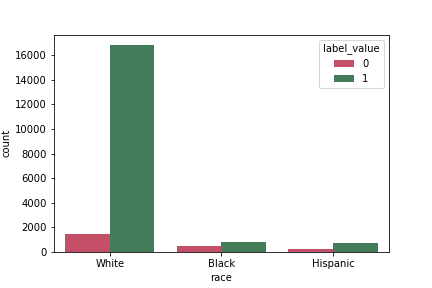
\includegraphics[width=\linewidth]{images/label_race_law_2.png}
    \endminipage\hfill
    \minipage{0.53\textwidth}%
      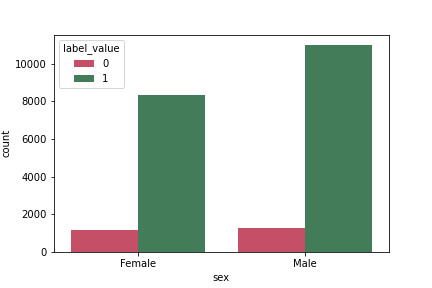
\includegraphics[width=\linewidth]{images/label_sex_law_2.png}
    \endminipage
     \caption{Distribución de las etiquetas reales para los atributos protegidos.}
     \label{fig:labelracesex2}
\end{figure}

\begin{figure}[H]
    \minipage{0.53\textwidth}
      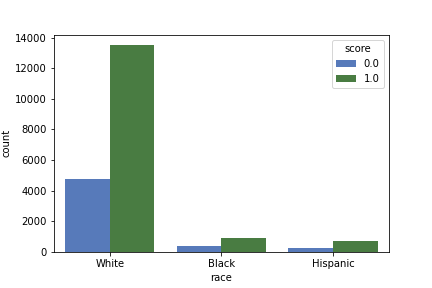
\includegraphics[width=\linewidth]{images/score_fair_k_race_law.png}
    \endminipage\hfill
    \minipage{0.53\textwidth}%
      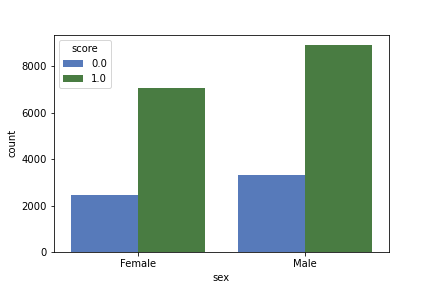
\includegraphics[width=\linewidth]{images/score_fair_k_sex_law.png}
    \endminipage
     \caption{Distribución de la puntuación para el modelo Fair $K$.}
     \label{fig:scorefairk}
\end{figure}

Existe un aumento de los individuos etiquetados negativamente que no viene reflejado en la Figura \ref{fig:labelracesex2}, por lo que podríamos contar con individuos que aun cumpliendo las condiciones de buena nota (\textit{label\_value}=1) obtuviese una predicción negativa (\textit{score}=0). Esta diferencia, entre predicciones y valor real, es la que influye en los malos resultados de este modelo para los valores de RMSE y $R^2$; sin embargo, esto se debe a que el modelo busca un equilibrio entre equidad-exactitud, por lo que sacrificamos la correcta clasificación de una parte de los individuos de la clase mayoritaria para evitar el sesgo hacia las clases minoritarias.

A continuación, definiremos las tablas para las métricas de grupo (Tabla \ref{tab:grupofairk}) y sesgo (Tabla \ref{tab:sesgofairk}), y para las medidas de equidad (Tabla \ref{tab:equidadfairk}) para el modelo Fair $K$.\\

\begin{table}[H]
\centering
\resizebox{13.cm}{!} {
\begin{tabular}{|c|c|c|c|c|c|c|c|c|}
\hline
\textbf{\begin{tabular}[c]{@{}c@{}}Nombre\\ del Atributo\end{tabular}} & \textbf{\begin{tabular}[c]{@{}c@{}}Valor\end{tabular}} & \textbf{PPR} & \textbf{FPR} & \textbf{TPR} & \textbf{PPV} & \textbf{NPV} & \textbf{FOR} & \textbf{FNR} \\ \hline
\textbf{race}                                                     & Asian                                                              & 0.04         & 0.54         & 0.74         & 0.86         & 0.29         & 0.71         & 0.26         \\ \hline
\textbf{race}                                                     & Black                                                              & 0.06         & 0.62         & 0.74         & 0.66         & 0.48         & 0.52         & 0.26         \\ \hline
\textbf{race}                                                     & Hispanic                                                           & 0.04         & 0.64         & 0.76         & 0.78         & 0.33         & 0.67         & 0.24         \\ \hline
\textbf{race}                                                     & Other                                                              & 0.02         & 0.46         & 0.78         & 0.87         & 0.39         & 0.61         & 0.22         \\ \hline
\textbf{race}                                                     & White                                                              & 0.84         & 0.56         & 0.76         & 0.94         & 0.14         & 0.86         & 0.24         \\ \hline
\textbf{sex}                                                      & Female                                                             & 0.44         & 0.57         & 0.77         & 0.91         & 0.21         & 0.79         & 0.23         \\ \hline
\textbf{sex}                                                      & Male                                                               & 0.56         & 0.58         & 0.75         & 0.92         & 0.16         & 0.84         & 0.25         \\ \hline
\end{tabular}
}
\caption{Métricas de grupo para el modelo Fair $K$.}
\label{tab:grupofairk}
\end{table}

\begin{table}[H]
\centering
\resizebox{16.cm}{!} {
\begin{tabular}{|c|c|c|c|c|c|c|c|c|}
\hline
\textbf{\begin{tabular}[c]{@{}c@{}}Nombre\\ del Atributo\end{tabular}} & \textbf{\begin{tabular}[c]{@{}c@{}}Valor\end{tabular}} & \textbf{\begin{tabular}[c]{@{}c@{}}PPR\\ Disparity\end{tabular}} & \textbf{\begin{tabular}[c]{@{}c@{}}FPR\\ Disparity\end{tabular}} & \textbf{\begin{tabular}[c]{@{}c@{}}TPR\\ Disparity\end{tabular}} & \textbf{\begin{tabular}[c]{@{}c@{}}PPV\\ Disparity\end{tabular}} & \textbf{\begin{tabular}[c]{@{}c@{}}NPV\\ Disparity\end{tabular}} & \textbf{\begin{tabular}[c]{@{}c@{}}FOR\\ Disparity\end{tabular}} & \textbf{\begin{tabular}[c]{@{}c@{}}FNR\\ Disparity\end{tabular}} \\ \hline
\textbf{race}                                                     & Asian                                                              & {\color[HTML]{FE0000} 0.05}                                      & {\color[HTML]{32CB00} 0.96}                                      & {\color[HTML]{32CB00} 0.97}                                      & {\color[HTML]{32CB00} 0.91}                                      & {\color[HTML]{FE0000} 2.07}                                      & {\color[HTML]{32CB00} 0.83}                                      & {\color[HTML]{32CB00} 1.08}                                      \\ \hline
\textbf{race}                                                     & Black                                                              & {\color[HTML]{FE0000} 0.07}                                      & {\color[HTML]{32CB00} 1.11}                                      & {\color[HTML]{32CB00} 0.97}                                      & {\color[HTML]{FE0000} 0.70}                                      & {\color[HTML]{FE0000} 3.43}                                      & {\color[HTML]{FE0000} 0.60}                                      & {\color[HTML]{32CB00} 1.08}                                      \\ \hline
\textbf{race}                                                     & Hispanic                                                           & {\color[HTML]{FE0000} 0.05}                                      & {\color[HTML]{32CB00} 1.14}                                      & {\color[HTML]{32CB00} 1.0}                                       & {\color[HTML]{32CB00} 0.83}                                      & {\color[HTML]{FE0000} 2.36}                                      & {\color[HTML]{FE0000} 0.78}                                      & {\color[HTML]{32CB00} 1.0}                                       \\ \hline
\textbf{race}                                                     & Other                                                              & {\color[HTML]{FE0000} 0.02}                                      & {\color[HTML]{32CB00} 0.82}                                      & {\color[HTML]{32CB00} 1.03}                                      & {\color[HTML]{32CB00} 0.93}                                      & {\color[HTML]{FE0000} 2.79}                                      & {\color[HTML]{FE0000} 0.71}                                      & {\color[HTML]{32CB00} 0.92}                                      \\ \hline
\textbf{race}                                                     & White                                                              & {\color[HTML]{3166FF} 1.0}                                       & {\color[HTML]{3166FF} 1.0}                                       & {\color[HTML]{3166FF} 1.0}                                       & {\color[HTML]{3166FF} 1.0}                                       & {\color[HTML]{3166FF} 1.0}                                       & {\color[HTML]{3166FF} 1.0}                                       & {\color[HTML]{3166FF} 1.0}                                       \\ \hline
\textbf{sex}                                                      & Female                                                             & {\color[HTML]{FE0000} 0.79}                                      & {\color[HTML]{32CB00} 0.98}                                      & {\color[HTML]{32CB00} 1.03}                                      & {\color[HTML]{32CB00} 0.99}                                      & {\color[HTML]{FE0000} 1.31}                                      & {\color[HTML]{32CB00} 0.94}                                      & {\color[HTML]{32CB00} 0.92}                                      \\ \hline
\textbf{sex}                                                      & Male                                                               & {\color[HTML]{3166FF} 1.0}                                       & {\color[HTML]{3166FF} 1.0}                                       & {\color[HTML]{3166FF} 1.0}                                       & {\color[HTML]{3166FF} 1.0}                                       & {\color[HTML]{3166FF} 1.0}                                       & {\color[HTML]{3166FF} 1.0}                                       & {\color[HTML]{3166FF} 1.0}                                       \\ \hline
\end{tabular}
}
\caption{Métricas de sesgo para el modelo Fair $K$.}
\label{tab:sesgofairk}
\end{table}

\begin{table}[H]
\centering
\resizebox{15.5cm}{!} {
\begin{tabular}{|c|c|c|c|c|c|c|c|}
\hline
\textbf{\begin{tabular}[c]{@{}c@{}}Nombre\\ del Atributo\end{tabular}} & \textbf{\begin{tabular}[c]{@{}c@{}}PPR\\ Disparity\end{tabular}} & \textbf{\begin{tabular}[c]{@{}c@{}}FPR\\ Disparity\end{tabular}} & \textbf{\begin{tabular}[c]{@{}c@{}}TPR\\ Disparity\end{tabular}} & \textbf{\begin{tabular}[c]{@{}c@{}}PPV\\ Disparity\end{tabular}} & \textbf{\begin{tabular}[c]{@{}c@{}}NPV\\ Disparity\end{tabular}} & \textbf{\begin{tabular}[c]{@{}c@{}}FOR\\ Disparity\end{tabular}} & \textbf{\begin{tabular}[c]{@{}c@{}}FNR\\ Disparity\end{tabular}} \\ \hline
\textbf{race}                                                     & {\color[HTML]{FE0000} FALSE}                                     & {\color[HTML]{32CB00} TRUE}                                      & {\color[HTML]{32CB00} TRUE}                                      & {\color[HTML]{FE0000} FALSE}                                     & {\color[HTML]{FE0000} FALSE}                                     & {\color[HTML]{FE0000} FALSE}                                     & {\color[HTML]{32CB00} TRUE}                                      \\ \hline
\textbf{sex}                                                      & {\color[HTML]{FE0000} FALSE}                                     & {\color[HTML]{32CB00} TRUE}                                      & {\color[HTML]{32CB00} TRUE}                                      & {\color[HTML]{32CB00} TRUE}                                      & {\color[HTML]{FE0000} FALSE}                                     & {\color[HTML]{32CB00} TRUE}                                      & {\color[HTML]{32CB00} TRUE}                                      \\ \hline
\end{tabular}
}
\caption{Medidas de equidad para el modelo Fair $K$.}
\label{tab:equidadfairk}
\end{table}

\subsubsection*{Modelo de error aditivo (Fair $Add$)}

Para este modelo obtenemos unos resultados muy similares a los del modelo Fair $K$. A simple vista, la única diferencia notable entre estos dos modelos la podemos observar comparando los gráficos de la Figura \ref{fig:scorefairadd} y los de la Figura \ref{fig:scorefairk}. Comentaremos si existen diferencias más notables relativas al cumplimiento de los criterios de equidad más adelante.\\

\begin{figure}[h]
    \minipage{0.53\textwidth}
      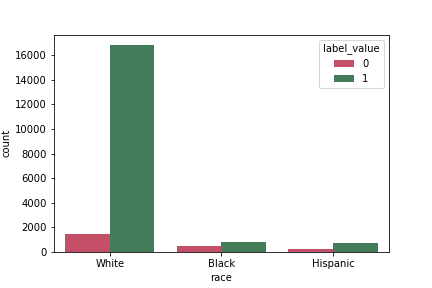
\includegraphics[width=\linewidth]{images/label_race_law_2.png}
    \endminipage\hfill
    \minipage{0.53\textwidth}%
      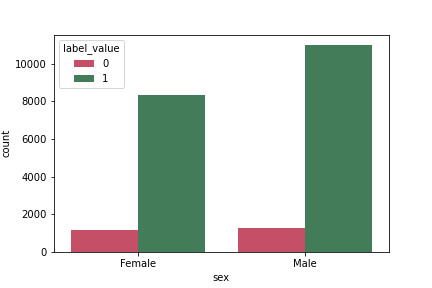
\includegraphics[width=\linewidth]{images/label_sex_law_2.png}
    \endminipage
     \caption{Distribución de las etiquetas reales para los atributos protegidos.}
     \label{fig:labelracesex1}
\end{figure}

\begin{figure}[h]
    \minipage{0.53\textwidth}
      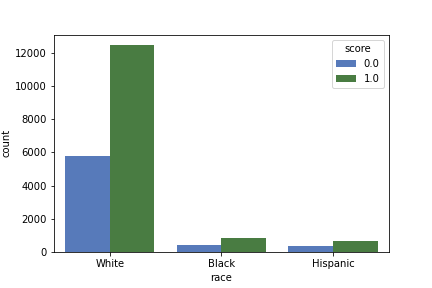
\includegraphics[width=\linewidth]{images/score_fair_add_race_law.png}
    \endminipage\hfill
    \minipage{0.53\textwidth}%
      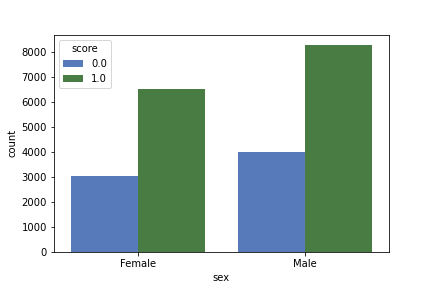
\includegraphics[width=\linewidth]{images/score_fair_add_sex_law.png}
    \endminipage
     \caption{Distribución de la puntuación para el modelo Fair $Add$.}
     \label{fig:scorefairadd}
\end{figure}

Seguidamente, presentaremos las tablas para las métricas de grupo (Tabla \ref{tab:grupofairadd}) y sesgo (Tabla \ref{tab:sesgofairadd}) para el modelo Fair $Add$. Como hemos hecho para el resto de modelos, también incluiremos el análisis para las medidas de equidad (Tabla \ref{tab:equidadfairadd}).\\

\begin{table}[h]
\centering
\resizebox{13.cm}{!} {
\begin{tabular}{|c|c|c|c|c|c|c|c|c|}
\hline
\textbf{\begin{tabular}[c]{@{}c@{}}Nombre\\ del Atributo\end{tabular}} & \textbf{\begin{tabular}[c]{@{}c@{}}Valor\end{tabular}} & \textbf{PPR} & \textbf{FPR} & \textbf{TPR} & \textbf{PPV} & \textbf{NPV} & \textbf{FOR} & \textbf{FNR} \\ \hline
\textbf{race}                                                     & Asian                                                              & 0.04         & 0.38         & 0.68         & 0.89         & 0.30         & 0.70         & 0.32         \\ \hline
\textbf{race}                                                     & Black                                                              & 0.06         & 0.50         & 0.77         & 0.71         & 0.58         & 0.42         & 0.23         \\ \hline
\textbf{race}                                                     & Hispanic                                                           & 0.04         & 0.44         & 0.73         & 0.83         & 0.42         & 0.58         & 0.27         \\ \hline
\textbf{race}                                                     & Other                                                              & 0.02         & 0.33         & 0.74         & 0.90         & 0.40         & 0.60         & 0.26         \\ \hline
\textbf{race}                                                     & White                                                              & 0.84         & 0.40         & 0.71         & 0.95         & 0.15         & 0.85         & 0.29         \\ \hline
\textbf{sex}                                                      & Female                                                             & 0.44         & 0.40         & 0.72         & 0.93         & 0.23         & 0.77         & 0.28         \\ \hline
\textbf{sex}                                                      & Male                                                               & 0.56         & 0.45         & 0.70         & 0.93         & 0.17         & 0.83         & 0.30         \\ \hline
\end{tabular}
}
\caption{Métricas de grupo para el modelo Fair $Add$.}
\label{tab:grupofairadd}
\end{table}

\begin{table}[H]
\centering
\resizebox{16.cm}{!} {
\begin{tabular}{|c|c|c|c|c|c|c|c|c|}
\hline
\textbf{\begin{tabular}[c]{@{}c@{}}Nombre\\ del Atributo\end{tabular}} & \textbf{\begin{tabular}[c]{@{}c@{}}Valor\end{tabular}} & \textbf{\begin{tabular}[c]{@{}c@{}}PPR\\ Disparity\end{tabular}} & \textbf{\begin{tabular}[c]{@{}c@{}}FPR\\ Disparity\end{tabular}} & \textbf{\begin{tabular}[c]{@{}c@{}}TPR\\ Disparity\end{tabular}} & \textbf{\begin{tabular}[c]{@{}c@{}}PPV\\ Disparity\end{tabular}} & \textbf{\begin{tabular}[c]{@{}c@{}}NPV\\ Disparity\end{tabular}} & \textbf{\begin{tabular}[c]{@{}c@{}}FOR\\ Disparity\end{tabular}} & \textbf{\begin{tabular}[c]{@{}c@{}}FNR\\ Disparity\end{tabular}} \\ \hline
\textbf{race}                                                     & Asian                                                              & {\color[HTML]{FE0000} 0.05}                                      & {\color[HTML]{32CB00} 0.95}                                      & {\color[HTML]{32CB00} 0.96}                                      & {\color[HTML]{32CB00} 0.94}                                      & {\color[HTML]{FE0000} 2.0}                                       & {\color[HTML]{32CB00} 0.82}                                      & {\color[HTML]{32CB00} 1.1}                                       \\ \hline
\textbf{race}                                                     & Black                                                              & {\color[HTML]{FE0000} 0.07}                                      & {\color[HTML]{32CB00} 1.25}                                      & {\color[HTML]{32CB00} 1.08}                                      & {\color[HTML]{FE0000} 0.75}                                      & {\color[HTML]{FE0000} 3.87}                                      & {\color[HTML]{FE0000} 0.49}                                      & {\color[HTML]{FE0000} 0.79}                                      \\ \hline
\textbf{race}                                                     & Hispanic                                                           & {\color[HTML]{FE0000} 0.05}                                      & {\color[HTML]{32CB00} 1.1}                                       & {\color[HTML]{32CB00} 1.03}                                      & {\color[HTML]{32CB00} 0.87}                                      & {\color[HTML]{FE0000} 2.8}                                       & {\color[HTML]{FE0000} 0.68}                                      & {\color[HTML]{32CB00} 0.93}                                      \\ \hline
\textbf{race}                                                     & Other                                                              & {\color[HTML]{FE0000} 0.02}                                      & {\color[HTML]{32CB00} 0.83}                                      & {\color[HTML]{32CB00} 1.04}                                      & {\color[HTML]{32CB00} 0.95}                                      & {\color[HTML]{FE0000} 2.67}                                      & {\color[HTML]{FE0000} 0.71}                                      & {\color[HTML]{32CB00} 0.9}                                       \\ \hline
\textbf{race}                                                     & White                                                              & {\color[HTML]{3166FF} 1.0}                                       & {\color[HTML]{3166FF} 1.0}                                       & {\color[HTML]{3166FF} 1.0}                                       & {\color[HTML]{3166FF} 1.0}                                       & {\color[HTML]{3166FF} 1.0}                                       & {\color[HTML]{3166FF} 1.0}                                       & {\color[HTML]{3166FF} 1.0}                                       \\ \hline
\textbf{sex}                                                      & Female                                                             & {\color[HTML]{FE0000} 0.79}                                      & {\color[HTML]{32CB00} 0.89}                                      & {\color[HTML]{32CB00} 1.03}                                      & {\color[HTML]{32CB00} 1.0}                                       & {\color[HTML]{FE0000} 1.35}                                      & {\color[HTML]{32CB00} 0.93}                                      & {\color[HTML]{32CB00} 0.93}                                      \\ \hline
\textbf{sex}                                                      & Male                                                               & {\color[HTML]{3166FF} 1.0}                                       & {\color[HTML]{3166FF} 1.0}                                       & {\color[HTML]{3166FF} 1.0}                                       & {\color[HTML]{3166FF} 1.0}                                       & {\color[HTML]{3166FF} 1.0}                                       & {\color[HTML]{3166FF} 1.0}                                       & {\color[HTML]{3166FF} 1.0}                                       \\ \hline
\end{tabular}
}
\caption{Métricas de sesgo para el modelo Fair $Add$.}
\label{tab:sesgofairadd}
\end{table}

\begin{table}[h]
\centering
\resizebox{15.5cm}{!} {
\begin{tabular}{|c|c|c|c|c|c|c|c|}
\hline
\textbf{\begin{tabular}[c]{@{}c@{}}Nombre\\ del Atributo\end{tabular}} & \textbf{\begin{tabular}[c]{@{}c@{}}PPR\\ Disparity\end{tabular}} & \textbf{\begin{tabular}[c]{@{}c@{}}FPR\\ Disparity\end{tabular}} & \textbf{\begin{tabular}[c]{@{}c@{}}TPR\\ Disparity\end{tabular}} & \textbf{\begin{tabular}[c]{@{}c@{}}PPV\\ Disparity\end{tabular}} & \textbf{\begin{tabular}[c]{@{}c@{}}NPV\\ Disparity\end{tabular}} & \textbf{\begin{tabular}[c]{@{}c@{}}FOR\\ Disparity\end{tabular}} & \textbf{\begin{tabular}[c]{@{}c@{}}FNR\\ Disparity\end{tabular}} \\ \hline
\textbf{race}                                                     & {\color[HTML]{FE0000} FALSE}                                     & {\color[HTML]{32CB00} TRUE}                                      & {\color[HTML]{32CB00} TRUE}                                      & {\color[HTML]{FE0000} FALSE}                                     & {\color[HTML]{FE0000} FALSE}                                     & {\color[HTML]{FE0000} FALSE}                                     & {\color[HTML]{FE0000} FALSE}                                     \\ \hline
\textbf{sex}                                                      & {\color[HTML]{FE0000} FALSE}                                     & {\color[HTML]{32CB00} TRUE}                                      & {\color[HTML]{32CB00} TRUE}                                      & {\color[HTML]{32CB00} TRUE}                                      & {\color[HTML]{FE0000} FALSE}                                     & {\color[HTML]{32CB00} TRUE}                                      & {\color[HTML]{32CB00} TRUE}                                      \\ \hline
\end{tabular}
}
\caption{Medidas de equidad para el modelo Fair $Add$.}
\label{tab:equidadfairadd}
\end{table}

\subsubsection*{Comparativa de las nociones de equidad}

Para concluir esta sección, presentaremos en la Tabla \ref{tab:equidadcomparativa} un resumen de los datos obtenidos para los cuatro modelos estudiados. Agruparemos las métricas de equidad en cuatro nociones de justicia, las cuales tres de ellas corresponden con las estudiadas en la Sección \ref{sec:groupmetrics}, y la última la presentamos en el Apéndice \ref{ap:herr_just}.

A la vista de los resultados, los modelos justos, a diferencia de los injustos, cumplen con el criterio de las probabilidades igualadas. Esto se debe, a que el cumplimiento de la equidad contrafactual impone de cierta forma un equilibrio entre las clases minoritarias y la mayoritaria. 


\clearpage

De esta forma, obtenemos individuos de raza blanca etiquetados incorrectamente, pero evitamos el sesgo en el resto de grupos demográficos. Es lógico, por tanto, que el criterio satisfecho sea el de probabilidades igualadas.\\

\begin{table}[h]
\centering
\resizebox{15.5cm}{!} {
\begin{tabular}{|c|c|c|cl|cl|cl|}
\hline
\textbf{Modelo}                            & \textbf{\begin{tabular}[c]{@{}c@{}}Nombre\\ del Atributo\end{tabular}} & \textbf{\begin{tabular}[c]{@{}c@{}}Paridad\\ Estadística\end{tabular}} & \multicolumn{2}{c|}{\textbf{\begin{tabular}[c]{@{}c@{}}Probabilidades\\ Igualadas\end{tabular}}} & \multicolumn{2}{c|}{\textbf{\begin{tabular}[c]{@{}c@{}}Tasa de Paridad\\ Predictiva\end{tabular}}} & \multicolumn{2}{c|}{\textbf{\begin{tabular}[c]{@{}c@{}}Paridad\\ Tipo II\end{tabular}}} \\ \hline
                                           & \textit{\textbf{race}}                                                 & {\color[HTML]{FE0000} FALSE}                                           & \multicolumn{2}{c|}{{\color[HTML]{FE0000} FALSE}}                                                & \multicolumn{2}{c|}{{\color[HTML]{FE0000} FALSE}}                                                  & \multicolumn{2}{c|}{{\color[HTML]{FE0000} FALSE}}                                       \\ \cline{2-9} 
\multirow{-2}{*}{\textbf{Completo}}        & \textit{\textbf{sex}}                                                  & {\color[HTML]{FE0000} FALSE}                                           & \multicolumn{2}{c|}{{\color[HTML]{FE0000} FALSE}}                                                & \multicolumn{2}{c|}{{\color[HTML]{32CB00} TRUE}}                                                   & \multicolumn{2}{c|}{{\color[HTML]{FE0000} FALSE}}                                       \\ \hline
                                           & \textit{\textbf{race}}                                                 & {\color[HTML]{FE0000} FALSE}                                           & \multicolumn{2}{c|}{{\color[HTML]{FE0000} FALSE}}                                                & \multicolumn{2}{c|}{{\color[HTML]{FE0000} FALSE}}                                                  & \multicolumn{2}{c|}{{\color[HTML]{FE0000} FALSE}}                                       \\ \cline{2-9} 
\multirow{-2}{*}{\textbf{Desconocimiento}} & \textit{\textbf{sex}}                                                  & {\color[HTML]{FE0000} FALSE}                                           & \multicolumn{2}{c|}{{\color[HTML]{32CB00} TRUE}}                                                 & \multicolumn{2}{c|}{{\color[HTML]{FE0000} FALSE}}                                                  & \multicolumn{2}{c|}{{\color[HTML]{32CB00} TRUE}}                                        \\ \hline
                                           & \textit{\textbf{race}}                                                 & {\color[HTML]{FE0000} FALSE}                                           & \multicolumn{2}{c|}{{\color[HTML]{32CB00} TRUE}}                                                 & \multicolumn{2}{c|}{{\color[HTML]{FE0000} FALSE}}                                                  & \multicolumn{2}{c|}{{\color[HTML]{FE0000} FALSE}}                                       \\ \cline{2-9} 
\multirow{-2}{*}{\textbf{Fair K}}          & \textit{\textbf{sex}}                                                  & {\color[HTML]{FE0000} FALSE}                                           & \multicolumn{2}{c|}{{\color[HTML]{32CB00} TRUE}}                                                 & \multicolumn{2}{c|}{{\color[HTML]{FE0000} FALSE}}                                                  & \multicolumn{2}{c|}{{\color[HTML]{32CB00} TRUE}}                                        \\ \hline
                                           & \textit{\textbf{race}}                                                 & {\color[HTML]{FE0000} FALSE}                                           & \multicolumn{2}{c|}{{\color[HTML]{32CB00} TRUE}}                                                 & \multicolumn{2}{c|}{{\color[HTML]{FE0000} FALSE}}                                                  & \multicolumn{2}{c|}{{\color[HTML]{FE0000} FALSE}}                                       \\ \cline{2-9} 
\multirow{-2}{*}{\textbf{Fair Add}}        & \textit{\textbf{sex}}                                                  & {\color[HTML]{FE0000} FALSE}                                           & \multicolumn{2}{c|}{{\color[HTML]{32CB00} TRUE}}                                                 & \multicolumn{2}{c|}{{\color[HTML]{FE0000} FALSE}}                                                  & \multicolumn{2}{c|}{{\color[HTML]{32CB00} TRUE}}                                        \\ \hline
\end{tabular}
}
\caption{Tabla comparativa para todos los modelos de equidad.}
\label{tab:equidadcomparativa}
\end{table}

Por otro lado, podemos observar cómo en ninguno de los casos se satisfacen simultáneamente los tres criterios de equidad de grupo. Esto corrobora el teorema de la imposibilidad (Capítulo \ref{ch:teoremaimposibilidad}), y hace evidente la idea de incompatibilidad de las tres nociones de grupo presentadas.

Podemos comprobar que la paridad de tipo II se satisface para el atributo sexo en los modelos justos, pero también en el modelo por desconocimiento, el cual también cumple para este atributo el criterio de probabilidades igualadas. Esto constata las gráficas presentadas en el Apartado \ref{subsec:graficas}; las cuales, para el atributo sexo eran justas contrafactualmente. El modelo completo sólo cumple la tasa de paridad predictiva para el atributo sexo; esto se debe a que al predecir con la información completa del problema (por ello obtiene la mejor tasa de RMSE), tiene buena actuación para el etiquetado de los individuos de la clase positiva (Precisión), y una proporción equilibrada para los de la negativa respecto al grupo de referencia (NPV Disparity). Por lo que, al cumplir las medidas de paridad para PPV y NPV simultáneamente, cumplirá la tasa de paridad predictiva.

Cabe destacar que, si tuviésemos que elegir entre un modelo justo para aplicarlo en un problema, el modelo de error aditivo (Fair $Add$) sería la mejor opción. Además de que es mucho más rápido en ejecución que el modelo Fair $K$ (ya que éste necesita realizar el muestreo con MCMC), cumple las mismas nociones de justicia y además, como observamos en la Tabla \ref{tab:coeficientes}, tiene mejores tasas de predicción sobre los datos originales. El único inconveniente, es que parte de suposiciones más fuertes, que necesitán del conocimiento del conjunto total de los datos, el cual podría no ser conocido en determinados casos.

\section{Condiciones de la experimentación}

En esta sección se hará un repaso de los diferentes entornos en los que se ha trabajado para la elaboración de este experimento, así como las bibliotecas que se utilizan para la programación del mismo.

\subsection{Entorno de ejecución}

Los experimentos realizados en este capítulo se han ejecutado en un equipo con las siguientes características:

\begin{itemize}
    \item Arquitectura x86\_64.
    \item AMD Ryzen 7 4800H with Radeon Graphics 2.90 GHz.
    \item 8 núcleos con 2 hilos de procesamiento por núcleo.
    \item 16 GB RAM DDR4.
    \item Sistema Operativo: Ubuntu 20.04.2 LTS.
\end{itemize}

\subsection{Entorno de programación}

\href{https://docs.spyder-ide.org/current/index.html}{Spyder} es un potente entorno de desarrollo integrado (IDE) de código abierto para el lenguaje Python. Dispone de funciones avanzadas de edición, control interactivo de pruebas y depuración. Gracias a su intérprete interactivo de Python y su compatibilidad con bibliotecas como NumPy, SciPy o matplotlib, se ha convertido en uno de los entornos de programación para Python más populares. 

Spyder incluye soporte de herramientas interactivas para la inspección de datos e incorpora controles de calidad específicos de Python. Además puede instalarse a través del sistema de gestión de paquetes de código abierto \href{https://docs.anaconda.com/}{Anaconda}, considerándose un IDE multiplataforma.

\subsection{Bibliotecas y herramientas auxiliares}

Algunas de las bibliotecas más importantes utilizadas junto al número de sus versiones han sido:

\begin{itemize}
    \item Pandas 1.2.4
    \item NumPy 1.19.2
    \item Scikit-learn 0.24.2
    \item matplotlib 3.4.3
    \item seaborn 0.11.2
    \item Aequitas 0.42.0
    \item pathlib2 2.3.6
    \item Módulos usados incluidos en Python: pickle, copy, os.
\end{itemize}

Además se ha utilizado el módulo \href{https://pystan.readthedocs.io/en/latest}{PyStan} 2.19.1.1 que funciona como una interfaz de Python para el lenguaje de programación probabilística \href{https://mc-stan.org}{Stan}. El cual permite generar muestras de datos a partir de métodos que trabajan con cadenas de Markov (como MCMC) y crear modelos causales sobre los que operar gracias a la inferencia estadística Bayesiana.

\section{Tutorial de ejecución del experimento} \label{sec:manual}

Incluimos un tutorial de ejecución de los experimentos en el formato \href{https://jupyter.org/documentation}{Jupyter Notebook}. Un archivo de Jupyter Notebook es un documento JSON, que sigue un esquema versionado y que contiene una lista ordenada de celdas de entrada/salida que pueden contener código, gráficos y texto, generalmente terminado con la extensión ''.ipynb''. 

El tutorial de ejecución y el resto del código implementado, se puede encontrar en la carpeta \texttt{experimentos} del repositorio público del proyecto, al cual puede acceder desde el \href{https://github.com/danibolanos/TFG-Ensuring_Fairness_in_ML/blob/main/experimentos/tutorial.ipynb}{siguiente enlace}\footnote{https://github.com/danibolanos/TFG-Ensuring\_Fairness\_in\_ML/blob/main/experimentos/tutorial.ipynb}.

\ctparttext{\color{black}\begin{center}
Conclusiones extraídas a lo largo del desarrollo del proyecto y debate de posibles rutas de trabajo futuras para el mismo.
\end{center}}
\part{Conclusiones y Vías Futuras} \label{part:debate_fut}

\chapter{Conclusión} \label{ch:conclusion}

La revisión previa de diferentes ejemplos como los citados en \cite{prestamo2018}, \cite{contratar2015} o \cite{condena2016} nos da indicios de la importancia de detectar y mitigar el sesgo dentro de una población que pudiera ser usada como conjunto de entrenamiento, o modelo de predicción de una aplicación programada para resolver problemas del mundo real. 

En este documento, se ha realizado un análisis de los conceptos de equidad más comúnes en la literatura de justicia en aprendizaje automático, con el objetivo de valorar las ventajas e inconvenientes de cada uno. También se ha realizado un estudio de las herramientas software actuales enfocadas en la detección de sesgo y sus limitaciones en la práctica, tanto en falta de conceptos implementados como en sus facilidades de uso para cualquier usuario.

En principio, las nociones de equidad por desconocimiento o equidad individual, podrían parecer suficientes para evitar el sesgo de un conjunto de datos, pero como hemos visto, la correlación invisible entre los atributos protegidos y otras características, o la fuerte dependencia de una métrica de distancia definida entre individuos, los hacen dos conceptos que a pesar de ofrecer una aproximación simple al concepto de equidad, tienen muchas desventajas a la hora de aplicarlos en la práctica.

Los conceptos de equidad de grupo surgen como una definición más formal del concepto de equidad y, a diferencia de las medidas discutidas previamente, su definición a partir de probabilidades condicionadas podría confundirse con una aplicación ideal y precisa de las nociones de equidad provenientes de la literatura de las ciencias sociales, algo bastante lejos de la realidad. La incompatibilidad entre sus tres medidas principales, demostrada a partir del teorema de imposibilidad, que impide imponer restricciones fuertes de equidad sobre un conjunto de datos. La relajación de varios de los conceptos impuestos con el objetivo de facilitar la aplicación práctica de estas métricas; así como la característica observacional de las medidas, que impide la explicación de la causa del sesgo en el problema. Son algunos de los inconvenientes con los que tiene que lidiar el concepto de equidad de grupo.

\clearpage

Con la aparición del concepto de medidas causales, que surge como solución a los problemas consecuentes de los anteriores criterios de equidad descritos, definimos la equidad contrafactual como una subclase de las mismas. No obstante, la equidad contrafactual a pesar de tener ventajas, como dar una explicación de la causa del sesgo, también tiene algunos problemas evidentes. El concepto de equidad contrafactual implica un conocimiento previo tanto de la inferencia causal, como de varios de sus herramientas básicas de trabajo, tales como los modelos causales y los grafos. La definición de los contrafactuales también implica un conocimiento matemático amplio necesario antes de trabajar en este contexto. Además, la creación del grafo causal del problema debe ser realizada por un experto en sociología o demografía, por lo que podría ocasionar inconvenientes durante la programación de la aplicación. Sin embargo, como vemos en la práctica, este concepto en general consigue eliminar el sesgo existente en los datos, da una explicación de la causa del sesgo, y ofrece herramientas visuales para la correcta interpretación de los datos por parte de un usuario sin amplios conocimientos en programación.

Durante la fase experimental, hemos replicado un ejemplo de equidad contrafactual sobre un conjunto de datos, donde hemos visto que el concepto de equidad contrafactual, a pesar de que obtiene peores resultados en exactitud, respecto a otras nociones básicas como la equidad por desconocimiento, consigue ser mejor en términos de mitigación de sesgo. Además, podemos ver que si auditamos un conjunto, utilizando el software de Aequitas para las diferentes medidas de equidad de grupo antes y después de que el conjunto de datos sea entrenado usando un modelo causal, nos encontramos con resultados sorprendentes, en cuanto a la existencia del sesgo en determinados grupos demográficos.

Finalmente, la utilización de herramientas software para la detección de sesgo como Aequitas sobre varios conjuntos de datos, nos presenta la necesidad de utilizar algoritmos de optimización, como el replicado en el experimento, para trabajar con un conjunto de datos que pudiese integrar tratamientos injustos sobre grupos específicos de la población. Además, señala la evidente falta de herramientas de interacción y visualización de resultados que pudieran ser utilizados, tanto por científicos de datos, como por otros expertos relacionados con el ámbito de las ciencias sociales. La existencia de estas utilidades facilitarían una interfaz de trabajo más amigable, con el objetivo de mejorar la comunicación entre los expertos de las ramas sociales y tecnológicas.

Concluimos asegurando que los objetivos presentados al inicio del trabajo se han cumplido según las expectativas previstas. Sin embargo, como se podrá leer en el capítulo siguiente, han surgido muchas vías de desarrollo relacionadas con la implementación de nuevas herramientas de interacción y visualización en el ámbito del proyecto. Las cuales hecho en falta haber implementado, o al menos introducido en este trabajo.  

\chapter{Trabajos futuros} \label{ch:trabajos_fut}

En el campo del aprendizaje automático, los sistemas de detección de sesgo, así como el desarrollo de nuevos conceptos de equidad, está evolucionando rápidamente. Es un hecho que en el mundo actual es totalmente necesario el tratamiento de comportamientos injustos que pudiesen existir en los conjuntos de datos usados para predecir resultados y tomar decisiones sobre los mismos

A lo largo de este proyecto hemos hecho una revisión de todos los conceptos de equidad que existen en la actualidad, analizando las ventajas e inconvenientes de cada uno de ellos. Uno de los principales problemas, es la incompatibilidad entre diversas nociones de la equidad, que como ya estudiamos en el Capítulo \ref{ch:teoremaimposibilidad}, obligan a relajar las restricciones en determinados problemas, si queremos imponer varios conceptos de equidad de grupo simultáneamente.

Una de las líneas de trabajo que podríamos desarrollar en un futuro, es la iniciada en \cite{impossibilityth2021} y del cuál hemos hablado en la Sección \ref{sec:saravaku}. Añadir una variable de corrección al grafo causal que elimine la incompatibilidad entre la paridad demográfica y el criterio de probabilidades igualadas, puede ser interesante a la hora de aplicarlo a determinados problemas con el objetivo de que el modelo use la información del atributo protegido, mientras evita un abuso del mismo de manera discriminatoria.

A raíz del estudio realizado en el Apéndice \ref{ap:herr_just} sobre diferentes paquetes de software para garantizar justicia en \textit{machine learning}, hemos podido comprobar que actualmente existen diversas herramientas para satisfacer la equidad en este ámbito. Como comentamos previamente, este tema es de evolución acelerada, y hay muchas instituciones públicas y privadas e investigadores interesados en el mismo, por lo que la construcción de herramientas progresa muy rápidamente. No obstante, hemos detectado la ausencia de utilidades para facilitar el trabajo a los científicos de datos, y expertos de otras ramas sin conocimientos realmente avanzados en programación. A continuación, proponemos algunas posibles vías de desarrollo centradas en los conceptos de equidad individual y equidad contrafactual:

\subsection*{Equidad individual}

Uno de los principales inconvenientes de esta noción es la fuerte dependencia a una métrica de distancia, definida entre los individuos de un conjunto de datos. El problema de esta métrica es que depende directamente del problema y en principio podría estar sesgada subjetivamente a la definición de la misma. Por ello proponemos una revisión desde la perspectiva matemática de diferentes clases de funciones que pudiesen generar unos pesos adecuados para cada individuo, y que no dependiesen en gran medida del problema en concreto, manteniendo un equilibrio razonable entre equidad y precisión de los resultados. 

Una vía de trabajo más práctica, sería construir un software que generase matrices de distancia con los pesos de los individuos, a partir de un conjunto de datos y unas especificaciones, determinadas por el experto en cuestión.

\subsection*{Equidad contrafactual}

La inferencia causal es un rama que no se restringe solamente a las matemáticas, si no que tiene un papel importante en otras ciencias tales como la sociología o medicina. En el ámbito de la equidad contrafactual, sería entonces de vital importancia implementar herramientas que pudiesen ser utilizadas de forma interactiva por expertos de estas otras ramas.

Actualmente existen implementaciones de paquetes como \href{https://xai-aniti.github.io/ethik/}{Ethik}, que incorporan diversos tratamientos y estudios gráficos para la noción de equidad contrafactual. Sin embargo, no muchos trabajos se centran en el apartado de la construcción del grafo causal, ya que esta tarea es normalmente desarrollada en el ámbito de la sociología política o demografía.

Proponemos el desarrollo de una aplicación que, haciendo uso de una biblioteca como \href{https://d3js.org/}{D3.js}, implemente una herramienta interactiva para construir los grafos causales y establecer las relaciones entre las diferentes variables, dado un \textit{dataset} con el problema. El software implementaría como \textit{FrontEnd}, tanto la construcción interactiva de los grafos causales como la visualización de resultados, en un entorno amigable para el usuario. En el \textit{BackEnd} se implementaría la construcción del modelo causal, haciendo uso, por ejemplo, del algoritmo utilizado en el experimento de la Parte \ref{part:analisis_exp}. De esta forma, se facilitaría la construcción de un grafo causal, el cual podría ser depurado por el propio experto. Obtendríamos una mejor comunicación entre las dos partes que colaboran (ciencias sociales e ingeniería), durante el desarrollo de modelos u algoritmos causales, y evitaríamos problemas en el diseño del grafo causal que pudiesen aparecer durante la implementación algorítmica.


\bibliographystyle{plainnat}
\bibliography{bibliography/research}

\addtocontents{toc}{\vspace{1\baselineskip}}

\addcontentsline{toc}{chapter}{\textsc{bibliografía}}

\ctparttext{\color{black}\begin{center}
\end{center}}
\part*{\textsc{Apéndices}}

\appendix
\chapter{Herramientas software para garantizar justicia}\label{ap:herr_just}
En este capítulo, hablaremos de algunas herramientas y técnicas que existen actualmente para garantizar la equidad en aprendizaje automático. Hablaremos de algunos de los más influyentes, entre los que destacaremos Aequitas por ser en el que nos vamos a basar en este trabajo. 

\section{Aequitas}

\textcolor{red}{NO REVISAR: Se completará con los experimentos usando la biblioteca de Aequitas}

Aequitas (\cite{aequitas2019}) es una herramienta de auditoría desarrollada por el \textit{Center for Data Science and Public Policy} de la
Universidad de Chicago. Es una herramienta de código abierto que consta de diversas utilidades de soporte para la auditoría de sesgos creado para ser utilizado por analistas de todo tipo relacionados con el ámbito del aprendizaje automático y cuyo principal objetivo es auditar los modelos de \textit{machine learning} con el fin de encontrar posibles discriminaciones en ellos y evitarlas en un futuro.

Aequitas nos permite detectar dos tipos de sesgos:

\begin{itemize}
    \item Acciones sesgadas que no ocurren de forma representativa en la población.
    \item Resultados sesgados a causa de errores de clasificación de nuestro sistema con respecto a ciertos grupos de la población.
\end{itemize}

Para utilizar la herramienta, se necesitan aportar los siguientes datos:

\begin{itemize}
    \item Datos sobre los atributos específicos (raza, sexo, etc.) que queramos auditar.
    \item El conjunto de personas de la población mencionada que el sistema de evaluación de riesgos seleccionó para una intervención.
\end{itemize}

\subsection{Estructura de los datos de entrada y resultados}

Podemos dividir en tres apartados (conformados por columnas en Aequitas) los datos que debemos aportar para el correcto funcionamiento de la herramienta.

\begin{itemize}
    \item \textbf{score}: representa la conclusión a la que llega un modelo, puede ser puede ser binaria ($0$ o $1$) o continua (decimal entre $0$ y $1$). Esta decisión representa si el sujeto es apto o no, por ejemplo, si se le concede un crédito bancario.
    \item \textbf{label\_value}: representa los datos reales, es decir, si la predicción realizada por el modelo fue correcta. Por ejemplo, el sujeto fue capaz de devolver el crédito en su totalidad. Es por esto, por lo que el modelo solo puede ser auditado después de su aplicación y no antes. Se representa como un valor binario, $1$ significa que la predicción fue correcta, $0$ que no lo fue.
    \item \textbf{attributes}: categorías de los atriburtos definidos por el usuario y utilizados para decidir la equidad del modelo. Algunos ejemplos de atributos son la raza, sexo, edad o ingresos.
\end{itemize}

\begin{table}[h]
\centering
\resizebox{12.0cm}{!} {
\begin{tabular}{|c|c|c|c|c|}
\hline
\textbf{score} & \textbf{label\_value} & \textbf{race}    & \textbf{sex} & \textbf{age\_cat} \\ \hline
0              & 1                     & Hispanic         & Male         & Less than 25      \\ \hline
1              & 0                     & African-American & Female       & 25-45             \\ \hline
0              & 0                     & Caucassian       & Male         & 25-45             \\ \hline
\end{tabular}
}
\caption{Ejemplo del \textit{dataset COMPAS} aportado a Aequitas.}
\label{tab:ejcompasaeq}
\end{table}



Para entender como funciona Aequitas, necesitamos presentar los siguientes conceptos preliminares definidos en: \url{https://dssg.github.io/aequitas/30_seconds_aequitas.html}

\begin{table}[h]
\centering
\resizebox{17.0cm}{!} {
\begin{tabular}{lll}
\hline
Nombre               & Notación                             & Definición                                                                                      \\ \hline
Score                & $S\in [0,1]$                         & puntuación de valor real asignada a cada entidad por el clasificador.                           \\
Decision             & $\hat{Y}\in \{0,1\}$                 & predicción binaria asignada a una entidad dada (\textit{data point}).          \\
True Outcome         & $Y\in \{0,1\}$                       & etiqueta binaria de una entidad dada.                                                           \\
Attribute            & $A=\{ a_i,a_2,\dots,a_n\}$           & atributo multivalor, por ejemplo., género=\{\textit{femenino,masculino,otro}\} \\
Group                & $g(a_i)$                             & todas las entidades que comparten el mismo valor de atributo, p. ej., género=femenino           \\
Reference group      & $g(a_r)$                             & uno de los grupos de $A$ que es usado como referencia para calcular las métricas de sesgo.      \\
Labeled Positive     & $LP_g$                               & número de entidades etiquetadas como positivas dentro de un grupo.                              \\
Labeled Negative     & $LN_g$                               & número de entidades etiquetadas como negativas dentro de un grupo.                              \\
Predicted Positive   & $PP_g$                               & número de entidades dentro de un grupo cuya predicción es positiva, es decir, $\hat{Y}=1$.        \\
Total Pred. Positive & $K=\sum_{A=a_1}^{A=a_n} PP_{g(a_i)}$ & número total de entidades $PP_g$ a lo largo de los grupos definidos por $A$.                    \\
Predicted Negative   & $PN_g$                               & número de entidades dentro de un grupo cuya predicción es negativa, es decir $\hat{Y}=0$.         \\
False Positive       & $FP_g$                               & número de entidades de un grupo con $\hat{Y}=1 \wedge Y=0$.                                     \\
False Negative       & $FN_g$                               & número de entidades de un grupo con $\hat{Y}=0 \wedge Y=1$.                                     \\
True Positive        & $TP_g$                               & número de entidades de un grupo con $\hat{Y}=1 \wedge Y=1$.                                     \\
True Negative        & $TN_g$                               & número de entidades de un grupo con $\hat{Y}=0 \wedge Y=0$.                                     \\ \hline
\end{tabular}
}
\caption{Conceptos preliminares de Aequitas.}
\label{tab:pretable}
\end{table}

La herramienta produce como resultado un informe en formato pdf que devuelve una interpretación descriptiva de los resultados junto con tres conjuntos de tablas con información relevante acerca de tres tipos de métricas:

\begin{itemize}
    \item Métricas de grupo.
    \item Métricas de sesgo.
    \item Medidas de equidad.
\end{itemize}

\subsection{Métricas usadas por Aequitas}

A continuación, veremos como se definen las diferentes métricas a partir de los conceptos preliminares definidos en el Cuadro \ref{tab:pretable}. Y mostraremos un ejemplo sobre el conjunto de datos \textit{COMPAS}.

\subsubsection{Métricas de grupo}

\begin{table}[h]
\centering
\resizebox{18.0cm}{!} {
\begin{tabular}{lll}
\hline
Nombre                  & Notación                                               & Definición                                                                                                                         \\ \hline
Prevalence              & $Prev_g=LP_g \ / \ \abs{g}=Pr(Y=1 \mid A=a_i)$        & \begin{tabular}[c]{@{}l@{}}fracción de entidades dentro de un grupo \\ cuyo valor real de la etiqueta fue positivo.\end{tabular}         \\
Predicted Prevalence    & $PPrev_g=PP_g \ / \ \abs{g}=Pr(\hat{Y}=1 \mid A=a_i)$ & \begin{tabular}[c]{@{}l@{}}fracción de entidades dentro de un grupo \\ que fue predicho como positivo.\end{tabular}                \\
Predicted Positive Rate & $PPR_g=PP_g \ / \ K=Pr(a=a_i \mid \hat{Y}=1)$         & \begin{tabular}[c]{@{}l@{}}fracción de entidades predichas como positivas \\ que pertenecen a un determinado grupo.\end{tabular}   \\
False Discovery Rate    & $FDR_g=FP_g \ / \ PP_g=Pr(Y=0 \mid \hat{Y}=1,A=a_i)$  & fracción de falsos positivos de un grupo entre el $PP_g$ del grupo.                                                                \\
False Omission Rate     & $FOR_g=FN_g \ / \ PN_g=Pr(Y=1 \mid \hat{Y}=0,A=a_i)$  & fracción de falsos negativos de un grupo entre el $PN_g$ del grupo.                                                                \\
False Positive Rate     & $FPR_g=FP_g \ / \ LN_g=Pr(\hat{Y}=1 \mid Y=0,A=a_i)$  & \begin{tabular}[c]{@{}l@{}}fracción de falsos positivos de un grupo \\ entre los etiquetados negativos del grupo.\end{tabular}     \\
False Negative Rate     & $FNR_g=FN_g \ / \ LP_g=Pr(\hat{Y}=0 \mid Y=1, A=a_i)$ & \begin{tabular}[c]{@{}l@{}}fracción de los falsos negativos de un grupo \\ entre los etiquetados positivos del grupo.\end{tabular} \\ \hline
\end{tabular}
}
\caption{Métricas de grupo de Aequitas.}
\label{tab:groupmetricaq}
\end{table}

Primero calcularemos el valor de las métricas de grupo para un atributo (p.ej. raza) teniendo en cuenta los conceptos del Cuadro \ref{tab:groupmetricaq}.

\begin{figure}[h]
	\centering
	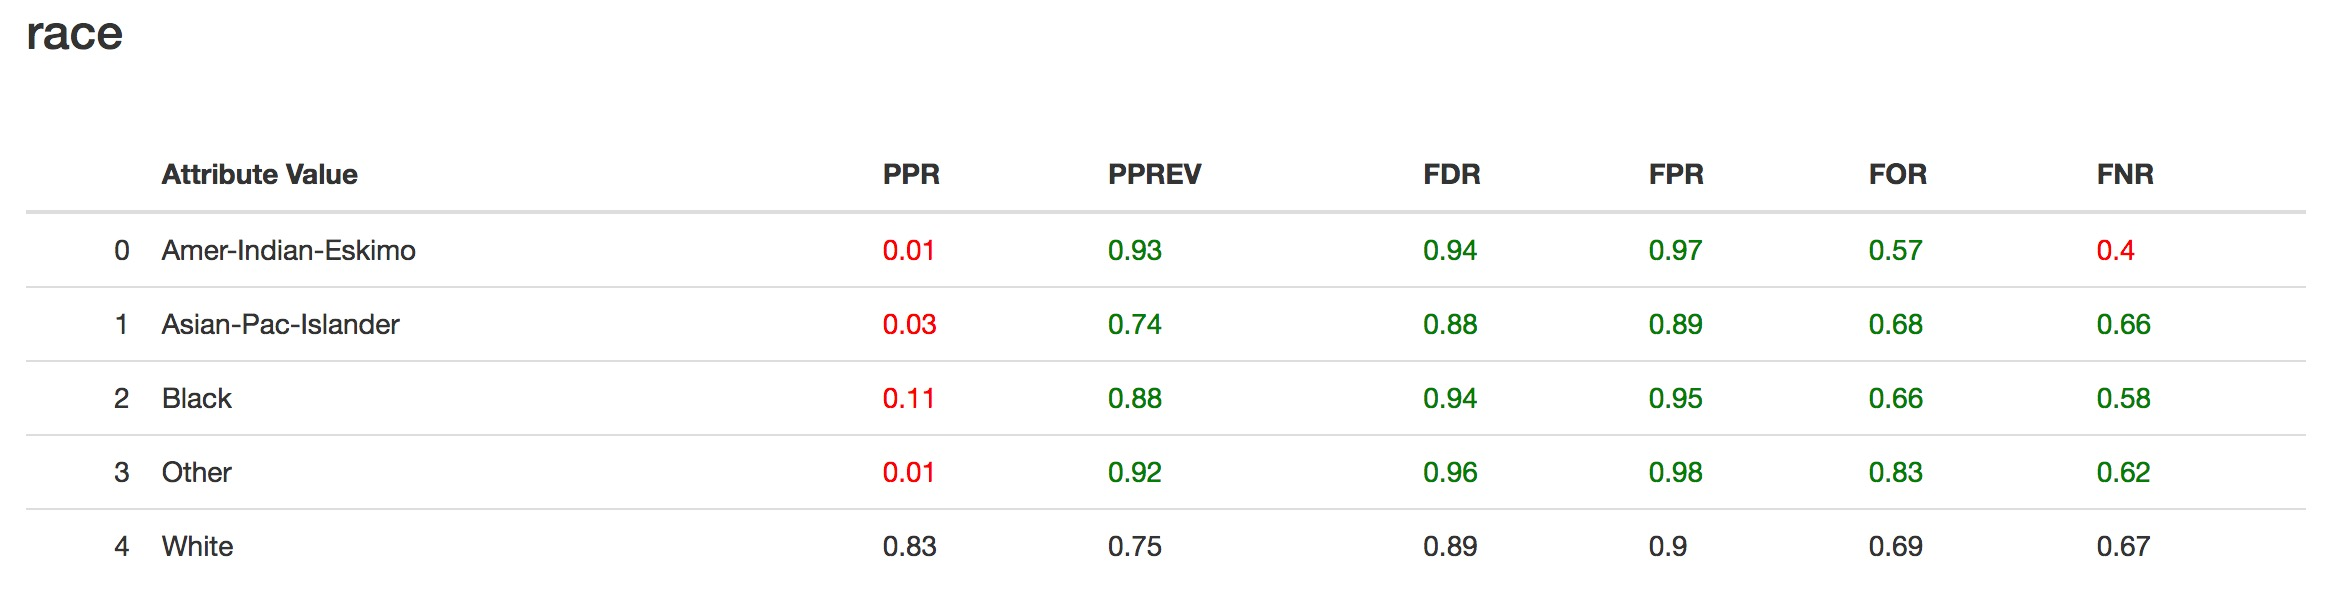
\includegraphics[width=17.5cm]{group_adult_aq.jpg}
	\caption{Tabla con las principales métricas de grupo para el atributo \textit{race}.}
    \label{fig:ejaq1}
\end{figure}

\subsubsection{Métricas de sesgo}

Mide la disparidad entre un grupo y el grupo de referencia. La disparidad se calcula a partir de la siguiente fórmula: $$DisparityMeasure_{ProtectedGroup}=\ddfrac{GroupMetric_{ProtectedGroup}}{GroupMetric_{ReferenceGroup}}$$ Donde $GroupMetric$ hace referencia a una métrica de grupo del Cuadro \ref{tab:groupmetricaq}. Es evidente que la disparidad de cualquier medida sobre el grupo de referencia siempre será 1. Si queremos calcular por ejemplo la disparidad del ratio de falsos negativos ($FNR$) sobre el grupo de raza negra, se calculará de la siguiente forma: $$FNR_{Black}=\ddfrac{FNR_{Black}}{FNR_{White}}=\ddfrac{0.58}{0.67}=0.86$$

Completando la tabla para todas las métricas de grupo obtenemos el siguiente resultado:

\begin{figure}[h]
	\centering
	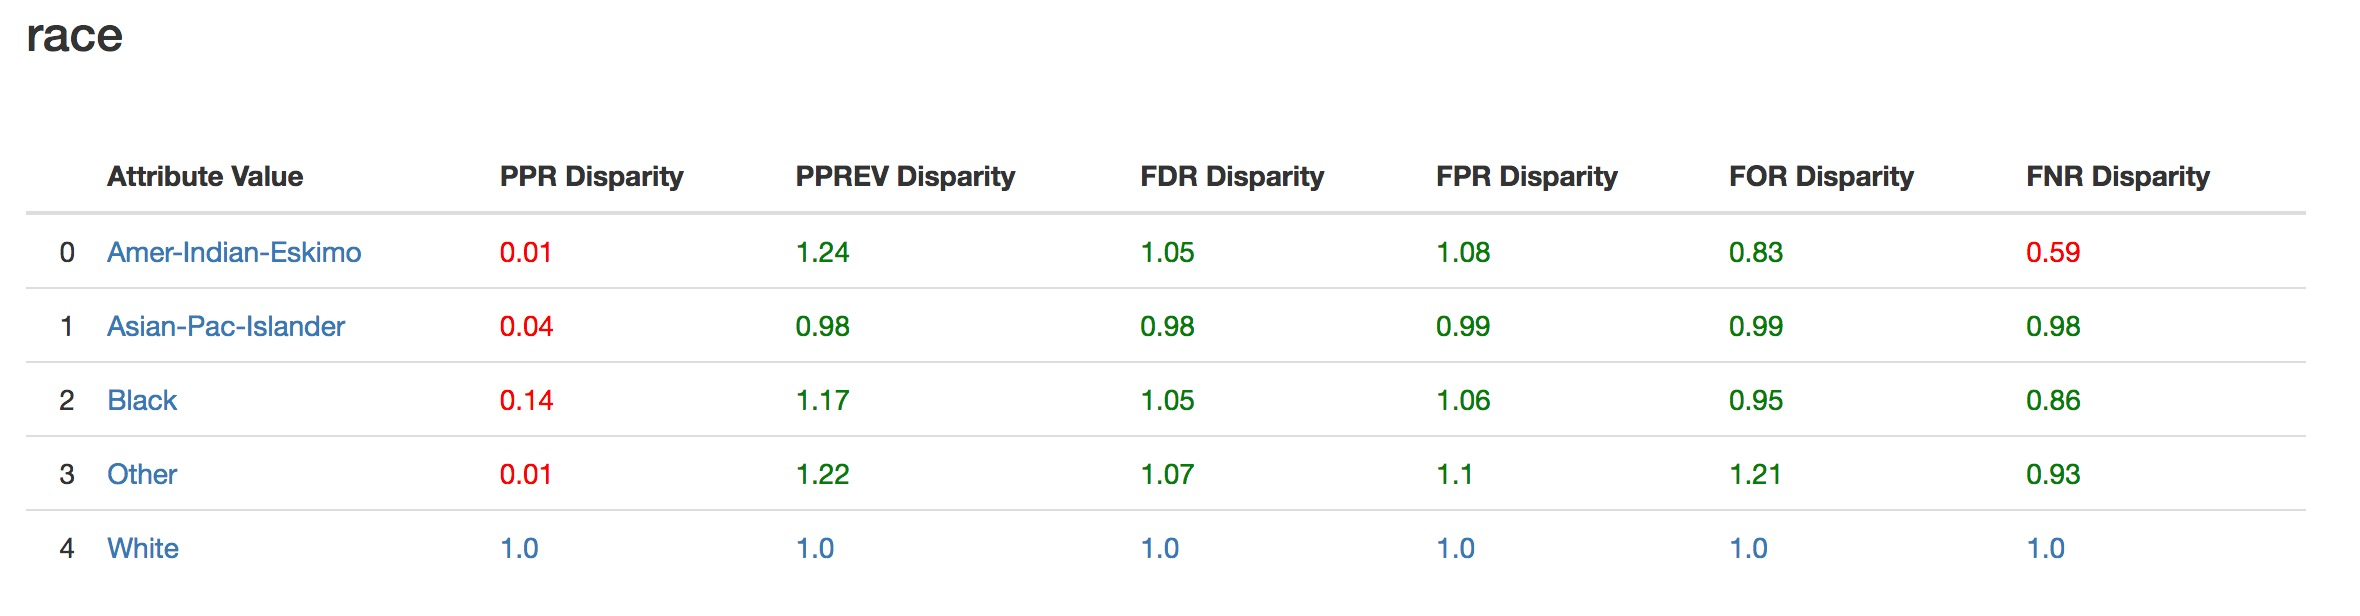
\includegraphics[width=17.5cm]{disparity_adult_aq.jpg}
	\caption{Tabla con las métricas de sesgo para el atributo \textit{race}.}
    \label{fig:ejaq2}
\end{figure}

\begin{remark}
De forma predeterminada, Aequitas usa el grupo mayoritario dentro de cada atributo como grupo de referencia.
\end{remark}

\subsubsection{Medidas de equidad}

La equidad siempre se define en relación con un grupo de referencia. Podemos ver que el cálculo de la equidad, depende de la métrica de sesgo. En la evaluación del criterio de equidad, un grupo cumple con la paridad si $$(1-\varepsilon)\leq \text{DisparityMeasure}_{\text{group}_i} \leq \ddfrac{1}{(1-\varepsilon)}$$ donde $\varepsilon$ es el umbral de equidad definido.

Tomando $\varepsilon=0.2$ cualquier métrica de sesgo se considerará justa en el intervalo $$\left[1-0.2,\ddfrac{1}{1-0,2}\right]=[0.8,1.25]$$

En el informe de resultados final que devuelve Aequitas si todas las métricas de equidad contienen el flag \textit{fair}, se evaluará el modelo actual como justo. De lo contrario, lo considerará injusto y enumerará los grupos afectados injustamente según los criterios de equidad dados.

\begin{figure}[h]
	\centering
	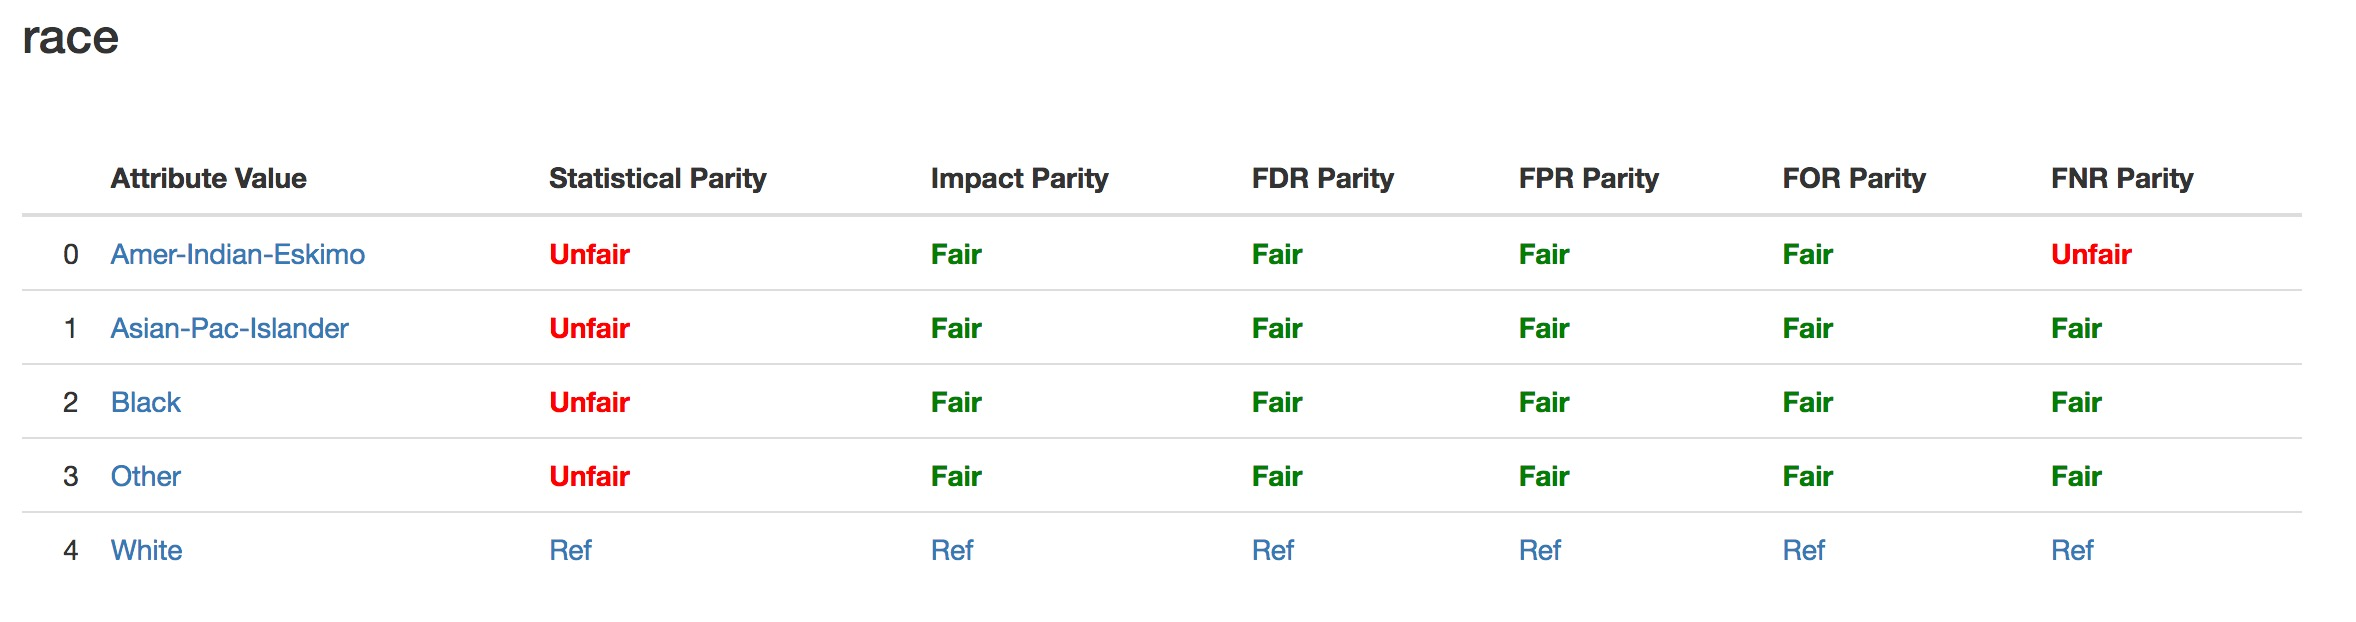
\includegraphics[width=17.5cm]{fairness_adult_output.jpg}
	\caption{Tabla de medidas de equidad aplicado el umbral.}
    \label{fig:medequmbral}
\end{figure}

\begin{figure}[h]
	\centering
	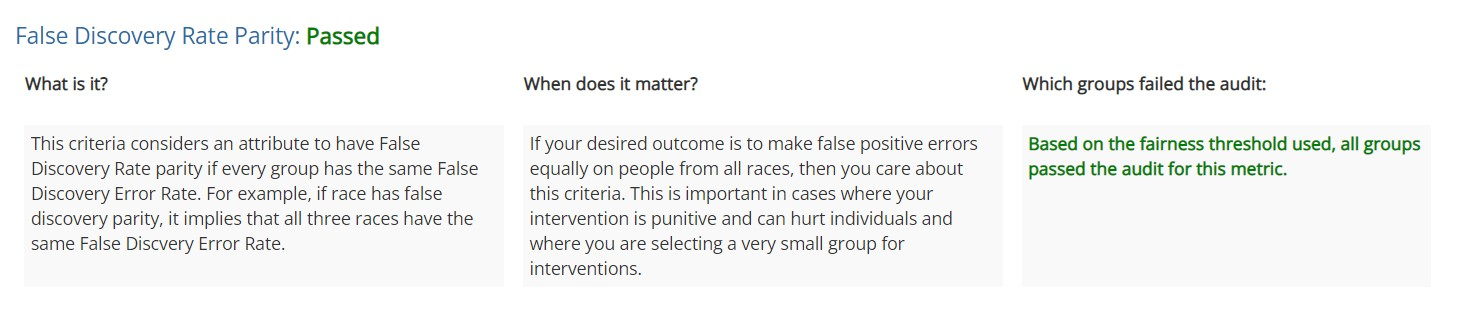
\includegraphics[width=17.5cm]{fairness_output_aq.jpg}
	\caption{Resultado del modelo injusto.}
    \label{fig:ejunfairaq}
\end{figure}

En la Figura \ref{fig:ejunfairaq} podemos ver que el modelo no cumple con los criterios de Paridad Falsa Negativa (\textit{False Negative Parity}) y de Igual Paridad (\textit{Equal Parity}).

Podemos ver que los conceptos de equidad que utiliza Aequitas son los siguientes:

\begin{itemize}
    \item Equal Parity.
    \item Proportional Parity.
    \item False Positive Parity.
    \item False Negative Parity.
\end{itemize}

\textcolor{red}{La versión actual es un esquema de lo que se intentará mostrar con imágenes sacadas de la web que deben cambiarse. Idea probar en Aequitas con las medidas existentes el mismo dataset que usaré con contrafactual, si no se puede, usar COMPAS.}

\chapter{Estimación del coste y planificación}\label{ap:coste_plan}
En este apéndice se realizará una estimación, tanto del coste como de la planificación del trabajo durante el período de desarrollo, con el objetivo de simular la valoración y presupuesto de un proyecto real en el ámbito laboral.

\section*{Estimación del presupuesto del proyecto}

Haremos un presupuesto del proyecto, en el que incluiremos las horas dedicadas a cada tema estudiado y realizaremos una estimación a precio 7 euros/hora. El análisis del presupuesto se puede observar en la Tabla \ref{tab:estcostes}.

Para facilitar la estimación de los costes, hemos dividido el trabajo en tres partes:

\begin{itemize}
    \item \textbf{Parte teórica}: recoge las tareas relacionadas con el análisis y el estudio de los conceptos de carácter teórico contenidos en el trabajo. Incluiremos la formalización de las nociones básicas para el proyecto y el desarrollo de las demostraciones matemáticas.
    \item \textbf{Parte práctica}: reúne las prácticas relacionadas con la programación, análisis y validación de los experimentos. Además tendremos en cuenta el equipo utilizado y los tiempos dedicados a instalación de bibliotecas y software empleados.
    \item \textbf{Parte general}: agrupa las labores de elaboración de la memoria y reuniones con los tutores (presencial u online).
\end{itemize}

El cómputo total es de 8.047 euros. Teniendo en cuenta que el período de trabajo útil ha sido de aproximadamente 5 meses, el sueldo medio mensual equivale a 1.609 euros brutos. Para un trabajador sin experiencia, este valor es bastante fiel a la realidad.

\section*{Planificación del trabajo}

El diseño de la planificación se ha realizado con el software \href{https://www.ganttproject.biz}{GanttProject}, que es un programa de código abierto utilizado para administrar proyectos, pudiendo usar entre otras muchas herramientas, un diagrama de Gantt. Para el desarrollo de la planificación, hemos usado la misma división en partes que la presentada en la sección anterior.

En la planificación original nos habría gustado presentar el trabajo para la convocatoria de septiembre, pero debido a algunos problemas derivados de la carga docente a lo largo del curso 2020-2021 y a la concreción de los experimentos asociados al proyecto, se ha acabado retrasando hasta el mes de noviembre.

Además es destacable, si comparamos las Figuras \ref{fig:planning_prev} y \ref{fig:planning}, que el tiempo dedicado tanto al estudio como la formalización de las diferentes medidas de equidad, ha sido mayor al previsto inicialmente.\\

\begin{figure}[h]
	\centering
	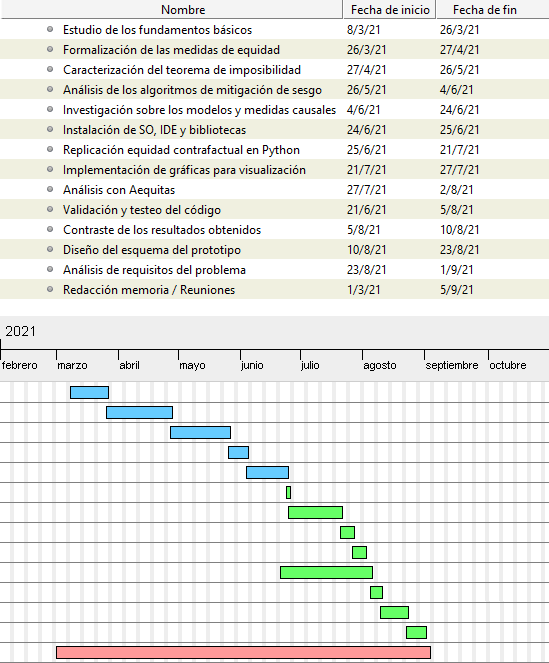
\includegraphics[width=12.7cm]{planificacion_prev.png}
	\caption{Planificación original del desarrollo del trabajo.}
    \label{fig:planning_prev}
\end{figure}

\clearpage

En ambos casos, la parte general es una tarea que se desarrolla a lo largo del período de trabajo, ya que la redacción de la memoria y las tutorías se realizan de forma simultánea al análisis teórico y práctico del proyecto. 

En la planificación final, hemos establecido el mes de abril como inicio del proyecto. Además el periodo de exámenes de junio también ralentizó en gran medida el avance del proyecto propuesto. Todos estos factores se pueden intuir observando la Figura \ref{fig:planning}, donde indicamos en color azul la parte teórica, en verde la parte práctica y en rojo la parte general.\\

\begin{figure}[h]
	\centering
	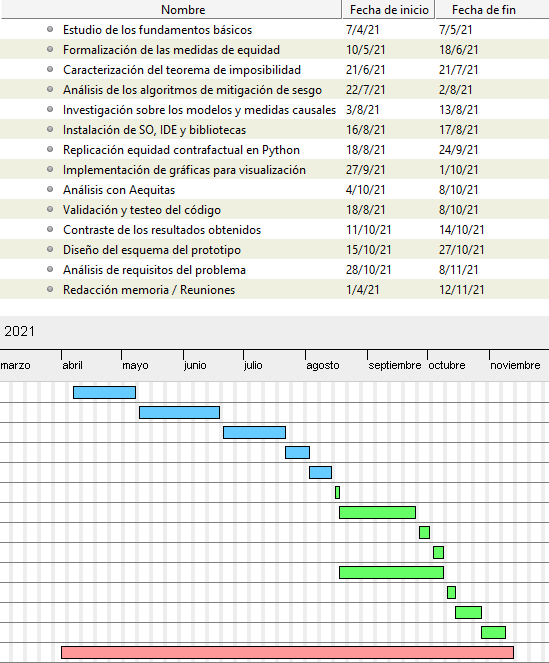
\includegraphics[width=12.7cm]{planificacion.png}
	\caption{Planificación final del desarrollo del trabajo.}
    \label{fig:planning}
\end{figure}

\begin{table}[h]
\centering
\resizebox{13.8cm}{!} {
\begin{tabular}{lccc}
\hline
\multicolumn{1}{c}{\textbf{Concepto}}                                                         & \begin{tabular}[c]{@{}c@{}}\textbf{Tiempo}\\ \textit{(horas)}\end{tabular} & \begin{tabular}[c]{@{}c@{}}\textbf{Coste} \\ \textit{(euros/hora)}\end{tabular} & \begin{tabular}[c]{@{}c@{}}\textbf{Coste total}\\ \textit{(euros)}\end{tabular} \\ \hline
\textbf{Parte general}                                                                        & \multicolumn{1}{l}{}                                     & \multicolumn{1}{l}{}                                         & \multicolumn{1}{l}{}                                          \\ \hline
Redacción de la memoria                                                                       & 300                                                      & 7                                                         & 2.100                                                            \\
Reuniones con los tutores                                                                     & 14                                                       &    -                                                        &   -                                                          \\ \hline
\textbf{Parte teórica}                                                                        & \multicolumn{1}{l}{}                                     & \multicolumn{1}{l}{}                                         & \multicolumn{1}{l}{}                                          \\ \hline
Estudio de los fundamentos básicos                                                                & 80                                                      & 7                                                          & 560                                                           \\
\begin{tabular}[c]{@{}l@{}}Formalización de las medidas \\ de equidad\end{tabular}            & 150                                                        & 7                                                          & 1.050                                                            \\
\begin{tabular}[c]{@{}l@{}}Caracterización del teorema \\ de imposibilidad\end{tabular}       & 90                                                       & 7                                                          & 630                                                            \\
\begin{tabular}[c]{@{}l@{}}Análisis de los algoritmos de \\ mitigación de sesgo\end{tabular}  & 32                                                        & 7                                                           & 224                                                           \\
\begin{tabular}[c]{@{}l@{}}Investigación sobre los \\ modelos y medidas causales\end{tabular}     & 45                                                        & 7                                                          & 315                                                           \\ \hline
\textbf{Parte práctica}                                                                       & \multicolumn{1}{l}{}                                     & \multicolumn{1}{l}{}                                         & \multicolumn{1}{l}{}                                          \\ \hline
Equipo de trabajo: ASUS TUF                                                                  &        -                                                 & -                                                           & 949                                                          \\
Instalación de SO, IDE y bibliotecas                                                           & 3                                                        & 7                                                           & 21                                                            \\
\begin{tabular}[c]{@{}l@{}}Replicación de un modelo de \\ equidad contrafactual en Python\end{tabular} & 120                                                        & 7                                                           & 840                                                            \\
\begin{tabular}[c]{@{}l@{}}Implementación de gráficas \\ para visualización\end{tabular}      & 16                                                       & 7                                                          & 112                                                           \\
Análisis con Aequitas                                                          & 28                                                      & 7                                                         & 196                                                           \\
Validación y testeo del código                                                                & 110                                                       & 7                                                          & 770                                                            \\
Contraste de los resultados obtenidos                                                         & 40                                                       & 7                                                          & 280                                                           \\ \hline
\textbf{Cómputo total del proyecto}                                                           & 1.028                                                       &    -                                                        & 8.047                                                           \\ \hline
\end{tabular}
}
\caption{Estimación del coste del proyecto.}
\label{tab:estcostes}
\end{table}

%\addtocontents{toc}{\vspace{1\baselineskip}}

%\clearpage

%\printglossary[title={\textsc{notación}}]
%\glsaddallunused


\end{document}